





\documentclass[12pt,a4paper]{article}
%\usepackage[top=0.85in,left=2.75in,footskip=0.75in]{geometry}
\usepackage[english]{babel}
\usepackage[utf8x]{inputenc}
\usepackage[T1]{fontenc}
\usepackage[a4paper]{geometry}
\geometry{a4paper, top=1in, bottom=2in}
\usepackage{amsmath}
\usepackage{amssymb}
\usepackage{graphicx}
\usepackage[colorlinks=true, allcolors=blue, hypertexnames=false]{hyperref}
\usepackage{epsfig,amsfonts}
\usepackage{natbib}
\usepackage{authblk}
\usepackage{subfig}
\usepackage{setspace}
\usepackage{hypcap}
\usepackage{lscape}
\usepackage{lineno} %can do [right] to shift location of #s
%From: https://www.overleaf.com/learn/how-to/Cross_referencing_with_the_xr_package_in_Overleaf
\usepackage{xr}
\makeatletter
\newcommand*{\addFileDependency}[1]{% argument=file name and extension
  \typeout{(#1)}
  \@addtofilelist{#1}
  \IfFileExists{#1}{}{\typeout{No file #1.}}
}
\makeatother
\newcommand*{\myexternaldocument}[1]{%
    \externaldocument{#1}%
    \addFileDependency{#1.tex}%
    \addFileDependency{#1.aux}%
}
%\myexternaldocument{Supplementary}
%From: https://tex.stackexchange.com/questions/64934/subfig-label-positioning (went with second example solution on how to get multiple figures aligned with subfig + desired labeling)
%\usepackage{floatrow}
%From: https://tex.stackexchange.com/questions/332295/command-textalpha-unavailable-in-encoding-t1-when-using-greek
\usepackage{textgreek}

%From Lorin
\usepackage{latexsym}
\usepackage{bm}
\usepackage{bbm}

\def\eq#1{(\ref{#1})}
\def\pdf{p.d.f.\ } \def\cdf{c.d.f.\ }
\def\pdfs{p.d.f.s} \def\cdfs{c.d.f.s}
\def\mgf{m.g.f.\ } \def\mgfs{m.g.f.s\ }
\def\ci{\perp   \perp}  % conditional independence symbol
\def\beginmat{ \left( \begin{array} }
\def\endmat{ \end{array} \right) }
\def\diag{{\rm diag}}
\def\log{{\rm log}}
\def\tr{{\rm tr}}
\def\cond{\, | \,}
\newcommand*\diff{\mathop{}\!\mathrm{d}}
%\newcolumntype{P}[1]{>{\centering\arraybackslash}p{#1}}

\def\dsum{\displaystyle\sum}
\def\dint{\displaystyle\int}
%\def\dfrac{\displaystyle\frac}
\def\dsup{\displaystyle\sup}
\def\dinf{\displaystyle\inf}
\def\dmin{\displaystyle\min}
\def\dlim{\displaystyle\lim}

\newcommand{\me}{\mathrm{e}}
\newcommand{\supp}{\operatorname{supp}}
\newcommand{\abs}[1]{\left|#1\right|}
\newcommand{\comment}[1]{{\em #1}}
\newcommand{\ba}{\mathbf{a}}
\newcommand{\bb}{\mathbf{b}}
\newcommand{\bc}{\mathbf{c}}
\newcommand{\be}{\mathbf{e}}
\newcommand{\bg}{\mathbf{g}}
\newcommand{\bl}{\mathbf{l}}
\newcommand{\bs}{\mathbf{s}}
\newcommand{\bt}{\mathbf{t}}
\newcommand{\bq}{\mathbf{q}}
\newcommand{\bk}{\mathbf{k}}
\newcommand{\bv}{\mathbf{v}}
\newcommand{\bx}{\mathbf{x}}
\newcommand{\by}{\mathbf{y}}
\newcommand{\bz}{\mathbf{z}}
\newcommand{\bh}{\mathbf{h}}
\newcommand{\bu}{\mathbf{u}}
\newcommand{\bw}{\mathbf{w}}
\newcommand{\w}{\mathbf{w}}
%\newcommand{\bm}{\mathbf{m}}
\newcommand{\bp}{\mathbf{p}}
\newcommand{\bK}{\mathbf{K}}
\newcommand{\bV}{\mathbf{V}}
\newcommand{\bA}{\mathbf{A}}
\newcommand{\bB}{\mathbf{B}}
\newcommand{\bC}{\mathbf{C}}
\newcommand{\bX}{\mathbf{X}}
\newcommand{\bY}{\mathbf{Y}}
\newcommand{\bE}{\mathbf{E}}
\newcommand{\bG}{\mathbf{G}}
\newcommand{\bH}{\mathbf{H}}
\newcommand{\bP}{\mathbf{P}}
\newcommand{\bQ}{\mathbf{Q}}
\newcommand{\bR}{\mathbf{R}}
\newcommand{\bW}{\mathbf{W}}
\newcommand{\bM}{\mathbf{M}}
\newcommand{\bU}{\mathbf{U}}
\newcommand{\bZ}{\mathbf{Z}}
\newcommand{\bD}{\mathbf{D}}
\newcommand{\bI}{\mathbf{I}}
\newcommand{\bS}{\mathbf{S}}
\newcommand{\T}{\intercal}
\newcommand{\wt}{\widetilde}
\newcommand{\wh}{\widehat}

\newcommand{\E}{\mbox{E}}
\newcommand{\V}{\mbox{V}}

\newcommand{\bbE}{\mathbb{E}}

\newcommand{\bepsilon}{\boldsymbol\epsilon}
\newcommand{\bvarepsilon}{\boldsymbol\varepsilon}
\newcommand{\bbeta}{\boldsymbol\beta}
\newcommand{\bsigma}{\boldsymbol\sigma}
\newcommand{\tbbeta}{{\tilde{\boldsymbol\beta}}}
\newcommand{\tbeta}{{\tilde{\beta}}}
\newcommand{\bgamma}{\boldsymbol\gamma}
\newcommand{\bdelta}{\boldsymbol\delta}
\newcommand{\btheta}{\boldsymbol\theta}
\newcommand{\bpi}{\boldsymbol\pi}
\newcommand{\bpsi}{\boldsymbol\psi}
\newcommand{\blambda}{\boldsymbol\lambda}
\newcommand{\bphi}{\boldsymbol\phi}
\newcommand{\brho}{\boldsymbol\rho}
\newcommand{\balpha}{\boldsymbol\alpha}
\newcommand{\bmu}{\boldsymbol\mu}
\newcommand{\bomega}{\boldsymbol\omega}
\newcommand{\btau}{\boldsymbol\tau}
\newcommand{\bDelta}{\boldsymbol\Delta}
\newcommand{\bGamma}{\boldsymbol\Gamma}
\newcommand{\bOmega}{\boldsymbol\Omega}
\newcommand{\bSigma}{\boldsymbol\Sigma}
\newcommand{\bLambda}{\boldsymbol\Lambda}
\newcommand{\bTheta}{\boldsymbol\Theta}
\newcommand{\at}[2][]{#1|_{#2}}
\newcommand{\red}[1]{\textcolor{red}{#1}}
\newcommand{\blue}[1]{\textcolor{blue}{#1}}

\title{Pathway Analysis within Multiple Human Ancestries Reveals Novel Signals for Epistasis in Complex Traits}
\author[1,2,$\dag$]{Michael C. Turchin}
\author[1,3]{Gregory Darnell}
\author[1,4,5,*]{Lorin Crawford}
\author[1,2,*,$\dag$]{Sohini Ramachandran}
\affil[1]{Center for Computational Molecular Biology, Brown University}
\affil[2]{Department of Ecology and Evolutionary Biology, Brown University}
\affil[3]{Institute for Computational and Experimental Research in Mathematics, Brown University}
\affil[4]{Department of Biostatistics, Brown University}
\affil[5]{Center for Statistical Science, Brown University}
\affil[$\ast$]{indicates these authors contributed equally}
\affil[$^\dag$]{To whom correspondence should be addressed:
michael\_turchin@brown.edu

sramachandran@brown.edu}

\begin{document}
%\setlength{\footskip}{0cm}

\maketitle

\begin{abstract}\label{InterPath-Abstract}

Genome-wide association (GWA) studies have identified thousands of significant genetic associations in humans across a number of complex traits. However, the majority of these studies focus on linear additive relationships between genotypic and phenotypic variation. Epistasis, or non-additive genetic interactions, is often regarded as a major driver of both complex trait architecture and evolution in multiple model organisms; yet, this same phenomenon is not considered to be a significant factor underlying human complex traits. There are two possible reasons for this assumption. First, most large GWA studies are conducted solely with European cohorts, therefore limiting our understanding of broad-sense heritability for many complex traits to just one ancestry group. Second, current epistasis mapping methods commonly identify significant genetic interactions by exhaustively searching across all possible pairs of SNPs; in these frameworks, estimated epistatic effects size are often small and power can be low due to the multiple testing burden. Here, we present a case study that uses a novel region-based mapping approach to analyze functionally interacting sets of variants for the presence of epistatic effects (``MArginal ePIstasis Test for Regions'', or \href{https://github.com/mturchin20/MAPITR}{MAPIT-R}) across six diverse subgroups within the UK BioBank (African, British, Caribbean, Chinese, Indian, and Pakistani). Even with limited sample sizes, we find a total of 245 pathways within the KEGG and REACTOME databases that are significantly enriched for epistasis in the complex traits height and body mass index (BMI), with 67\% of these pathways being detected within the African subgroup. We find that BMI commonly produces greater evidence for epistatic interactions than height, and that, amongst the BMI significant pathways in the African subgroup, components of the proteasome are enriched for epistatic interactions. Further, using proteasome gene families, we show how to use a region-based `leave-one-out' approach to localize pathway-level interaction signals to more specific genes. Overall, our results indicate that non-European ancestry populations may be better suited for the discovery of epistatic signals in human complex traits---further underscoring the need for publicly available, biobank-sized datasets of diverse non-European individuals.

\end{abstract}

\linenumbers

\section{Introduction}\label{InterPath-Introduction}

Genome-wide association (GWA) studies are a powerful tool for identifying statistical associations between genetic variation and complex traits, and have identified over 70,000 statistically significant such associations in humans alone \citep{Buniello2019}. The most common approach for conducting GWA studies is testing for linear associations between genetic variants and a trait of interest, where estimated effect sizes represent an additive relationship between number of copies of a single-nucleotide polymorphism and the phenotypic state. While this approach has produced many additive associations, it is unable to detect nonlinear associations---such as epistasis between genetic variants---that also contribute to a trait's genetic architecture. Epistasis produces non-additive effects on a given trait and is a well-established phenomenon in a number of model organisms \citep{Lehner2006,Rowe2008,Shao2008,Flint2009,Costanzo2010,He2010,Jarvis2011,Pettersson2011,Bloom2013,Monnahan2015}. Epistasis has also been suggested as a major driver of both complex trait genetic architecture and evolution \citep{Carlborg2004,Carlborg2006,Martin2007,Phillips2008,Moore2009,Zuk2012,Jones2014,Mackay2014}. Still, there remains skepticism regarding the importance of epistasis in human complex traits and diseases \citep{Hill2008,Crow2010,Yang2010,Aschard2012,Powell2013,Maki-Tanila2014,Wood2014,Yang2015}. For example, multiple studies have suggested  that complex trait variation can be explained mainly with additive effects \citep{Hill2008,Crow2010,Maki-Tanila2014} (though the framework for doing so has been questioned \citep{Huang2016}). In initial work to locate the  ``missing heritability'' in the human genome -- the discrepancy between larger pedigree-based trait heritability estimates and smaller SNP-based trait heritability estimates using the first wave of human GWAS results \citep{Maher2008,Manolio2009,Eichler2010} -- it was suggested that epistasis may account for a significant portion of this observed discrepancy \citep{Slatkin2009,Zuk2012,Hemani2013}. However recent studies have suggested that, for at least some complex traits,  epistasis is unlikely to be a major contributor to total trait heritability \citep{Yang2015}.

Additionally, detecting epistasis via genome-wide scans is much more computationally costly than the hypothesis-generating GWA framework. GWA tests are linear in the number of SNPs, while epistasis scans consider, at a minimum, all pairwise combinations of SNPs. Recent work by \citet{Crawford2017a}, however, made significant computational improvements for detecting genetic interactions by introducing a completely new framework for identifying a specific type of epistasis, \textit{marginal epistasis}. %...Recent methodological advances have shown increasing evidence for epistasis in humans \citep{Verma2016,Crawford2017a,Fang2019,Runcie2019} 
Marginal epistasis refers to the total interaction effects of a single variant with all other variants genome-wide; marginal epistasis reduces the state space of epistasis tests by testing whether a single variant has any non-zero interaction effects with the remaining set of variants. 

\citet{Crawford2017a} implemented MAPIT, and focused on analyzing only single variants one at a time for marginal signals of epistasis with other variants in the rest of the genome. As with GWA studies though, identifying marginal signals of association is difficult to interpret biologically. One successful way GWA studies have addressed this issue is by expanding GWA frameworks to aggregate across multiple SNP-level association signals and test for enrichment of associations in genes and pathways \citep{Subramanian2005,Cantor2010,Wang2010b,Lee2012,Carbonetto2013,Mooney2014,Gamazon2015,de2016,Nakka2016,Zhu2018,Sun2019,Cheng2020}. In this study, our objective is to expand the marginal epistasis framework to test for enrichment of epistatic signals in user-specified groups of variants (e.g., genes, pathways), producing biologically interpretable scans for epistasis while reducing the multiple testing burden. We implement this new approach in ``MArginal ePIstasis Test for Regions'', which we refer to as MAPIT-R (\url{https://github.com/mturchin20/MAPITR}).

We apply MAPIT-R to genotype data and the quantitative measurements of standing height and body mass index (BMI) using pathways from the KEGG and REACTOME databases \citep{Liberzon2011} and samples from multiple human ancestry ``subgroups'' (British, African, Caribbean, Chinese, Indian, and Pakistani)  in the UK BioBank (UKB) dataset \citep{Sudlow2015}. We analyze multiple non-European human ancestries to study how varying genomic backgrounds might reveal epistatic interactions. We find over 200 pathways that have significant marginal epistatic interactions with the rest of the genome across both our phenotypes and UKB datasets. We then investigate the distribution of these significant epistatic signals across ancestries, traits, and pathways, which suggests future directions to prioritize for studies of epistasis in human complex traits.

\section{Results}\label{InterPath-Results}

%MT Org notes:
%
%Supp Table for dsc
%
%-'2.5\% PC1 tail thing'
%-'SR: also, do those describe why the pathway numbers change? Is it due to SNPs in pathways changing with QC procedures? I think that needs to be clarified in the caption.' for BritReps table (cmmnt)
%-grgSmltnFgr?

\subsection{Overview of the MAPIT-R Model}\label{InterPath-Results-MAPITRModel}

Here we provide an overview of the MAPIT-R model, a multiple-variant extension of the single-variant MAPIT framework (\citet{Crawford2017a}; see Materials and Methods for a full description). The objective of MAPIT-R is to test whether there are any non-zero genetic interaction effects between a group of variants $\textbf{R}$ and \textbf{any} other variant remaining in the genome ($\textbf{R}^C$). The typical GWA linear form of this model is:  
\begin{equation}\label{Overview1}
\textbf{y} = \mu\textbf{1} + \sum_{r \in R} \textbf{x}_r\beta_r + \sum_{s \not\in R} \textbf{x}_s\beta_s + \sum_{r \in R}\sum_{s \not\in R} (\textbf{x}_r \circ \textbf{x}_s)\alpha_{rs} + \boldsymbol{\epsilon}, \quad \boldsymbol{\epsilon} \sim \mathcal{MVN}(\textbf{0}, \tau^{2}\textbf{I})  
\end{equation}
where \textbf{y} is a $n \times 1$ vector of phenotypes, $\mu$ is the grand mean, $\textbf{x}_r$ is a $n \times 1$ vector of genotypes for each variant $r$ that belongs to the total group of variants $\textbf{R}$, $\beta_r$ is the additive effect size for each variant $r$, $\textbf{x}_s$ is a $n \times 1$ vector of genotypes for every variant $s$ that does not belong to the group $\textbf{R}$, $\beta_s$ is the additive effect size for each variant $s$, $(\textbf{x}_r \circ \textbf{x}_s)$ is the Hadamard product between the two variant genotype vectors $\textbf{x}_r$ and $\textbf{x}_s$, $\alpha_{rs}$ is interaction effect size between variants $r$ and $s$, and $\boldsymbol{\epsilon}$ is a $n \times 1$ vector of random effects which follow a multivariate normal distribution with mean $\textbf{0}$ and covariance matrix equal to variance effect $\tau$ times the $n \times n$ identity matrix $\textbf{I}$. Here the Hadamard product between variants in the sets belonging to and not belonging to \textbf{R} represent the genetic interactions between the variants in \textbf{R} and the rest of the genome.

However, we observe that the model in equation \ref{Overview1} is an underdetermined linear system ($p >> n$). Therefore, we make additional modeling assumptions on the effect sizes $\beta_r$, $\beta_s$, and $\alpha_{rs}$ to make the model identifiable. To do so, we follow standard approaches \citep{Wu2011,Zhou2013,Yang2010} and assume that each individual effect size follows a normal distribution: $\beta_r \sim \mathcal{N}(0, \omega^2/q)$, $\beta_s \sim \mathcal{N}(0, \sigma^2/(p-q))$, and $\alpha_{rs} \sim \mathcal{N}(0, \phi^2/(q*(p-q)))$, where $q$ is the number of variants in \textbf{R} and $p$ is the total number of variants in the dataset \citep{Crawford2017a}. With the normal assumption on effect sizes, the model in equation \ref{Overview1} becomes equivalent to the following variance component model:

\begin{align}\label{Overview2}
    & \textbf{y} = \mu + \textbf{K} + \textbf{M} + \textbf{G} + \boldsymbol{\epsilon} \\
    \textbf{K} \sim \mathcal{MVN}&(\textbf{0}, \phi^{2}\textbf{K}_K) \quad \textbf{M} \sim \mathcal{MVN}(\textbf{0}, \omega^{2}\textbf{K}_M) \nonumber \\ 
    \textbf{G} \sim \mathcal{MVN}&(\textbf{0}, \sigma^{2}\textbf{K}_G) \quad \boldsymbol{\epsilon} \sim \mathcal{MVN}(\textbf{0}, \tau^{2}\textbf{I}) \nonumber 
\end{align}
where \textbf{K}, \textbf{M}, and \textbf{G} are all random effects that follow multivariate normal distributions, $\phi$, $\omega$, and $\sigma$ are their respective variance components, $\textbf{K}_K = \textbf{X}_{R}\textbf{X}^{\textbf{T}}_{R}/q$, the genetic relatedness matrix (GRM) constructed from the $q$ variants that belong to $\textbf{R}$, $\textbf{K}_M = \textbf{X}_{-R}\textbf{X}^{\textbf{T}}_{-R}/(p-q)$, the GRM constructed from all the remaining variants in $p$ not in $\textbf{R}$, and $\textbf{K}_G = \textbf{K}_K \circ \textbf{K}_M$, the Hadamard product between the GRMs $\textbf{K}_K$ and $\textbf{K}_M$, representing the genetic interactions between the variants in $\textbf{R}$ and the rest of the genome.

Given this new, implementable form of our model, we return to our test of interest: whether there are any non-zero interaction effects between the variants in \textbf{R} and the rest of the genome. This is equivalent to testing whether the variance component $\sigma$ is equal to 0, or restated, to testing a null hypothesis of $H_0: \sigma = 0$. To estimate and test $\sigma$, we follow the same procedure as MAPIT and employ MQS, an approach that is based on the method of moments and produces estimates that are mathematically identical to the Haseman-Elston (HE) cross-product regression \citep{Haseman1972, Zhou2017} (see Materials and Methods). MQS allows us to jointly estimate the set of variance components $(\phi^{2}, \omega^{2}, \sigma^{2}, \tau^{2})$ in a computationally tractable manner, which are needed to both properly test $\sigma$ and be recalculated for every pathway. Given these variance component estimates per pathway then, we are able to test $\sigma$ and get final $p$-values using the Davies method \citep{Crawford2017a,Davies1980}.  

\subsection{Analyses of the African subgroup identify many pathways with significant marginal epistasis}\label{InterPath-Results-PathwayEpistasis}

We applied MAPIT-R to height and BMI to detect pathways from the KEGG and REACTOME databases \citep{Liberzon2011} with significant epistatic interactions with the rest of the genome, using genotype data and diverse individuals from the UK Biobank. We focused on height and BMI due to the extensive work that has already been done investigating the broad-sense and narrow-sense heritabilities of these traits \citep{Yang2010,Elks2012,Visscher2012,Finucane2015,Speed2017,Wainschtein2019}, and we used the KEGG and REACTOME databases because they cover an extensive range of biological processes as well as pathway-sizes (measured in SNP counts). We analyzed six different human ancestry subgroups that we extracted from the UKB: African (n=3111), British (n=3848, chosen randomly from 442,688), Caribbean (n=3833), Chinese (n=1448), Indian (n=5077), and Pakistani (n=1581) (Supplementary Figure \ref{InterPath-Supp-Figure-UKB-subgroups-PCAPlot} and Supplementary Table \ref{InterPath-Supp-Table-UKBPopStats}). Subgroups were extracted based on self-identified ancestry and individuals were filtered using standard quality control (QC) procedures (see Materials and Methods for details).

Applying MAPIT-R to height and BMI measurements and genotype data using these pathway databases and ancestry subgroups, we find 245 pathways that have genome-wide significant signals for marginal epistatic interactions with the rest of the genome (Figure \ref{InterPath-Main-Figure-Barplots-KEGG}, Supplementary Figure \ref{InterPath-Supp-Figure-Barplots-REACTOME}, and Supplementary Tables \ref{InterPath-Supp-Table-TopPathways-AllPaths-AllPhenos}\textcolor{blue}{a-d}; $p$-value significance thresholds were determined using Bonferroni multiple testing correction based on the number of pathways tested per analysis, see Supplementary Table \ref{InterPath-Supp-Table-UKBPopStats}). We find similar numbers of significant pathways between the KEGG and REACTOME databases: 130 and 115, respectively. Totaling across both databases, we find that BMI contains more significant pathways than does height: 155 versus 90, respectively. The majority of our significant results are identified in database-phenotype-subgroup analyses using the African subgroup: 165 out of 245 significant pathways across all database-phenotype-subgroup analyses.

The specific pathways with significant marginal epistasis signals in the African subgroup share multiple themes across each of the database-phenotype combinations (Supplementary Tables \ref{InterPath-Supp-Table-TopPathways-AllPaths-AllPhenos}\textcolor{blue}{a-d}). Focusing on height in KEGG, we find multiple pathways enriched for epistatic signals representing cellular signaling, immune systems, and heart conditions; in BMI, we find similar results as well as signals in multiple metabolic pathways (Table \ref{InterPath-Main-Table-KEGG-African-TopPathways-Themes}). Our results are similar to other work showing evidence for the importance of epistasis in human immunity, particularly involving the Major Histocompatibility Complex (MHC) \citep{Martin2002,Williams2005,Wan2010,Rose2012,Lareau2016,Opi2018,Zhang2019}, as well as metabolism and cellular signaling in model systems \citep{Segre2005,Snitkin2011,Podgornaia2015,Sorrells2015,Tyler2017,Nghe2018,Jiao2019}. Our results when analyzing REACTOME pathways show similar themes to our observations of epistatic signals in KEGG pathways (see Supplementary Tables \ref{InterPath-Supp-Table-TopPathways-AllPaths-AllPhenos}\textcolor{blue}{a-d} for complete lists of MAPIT-R significant pathways in all database-phenotype-subgroup combinations).  


\begin{figure}[htb]
\centering
\hspace*{-.9cm}
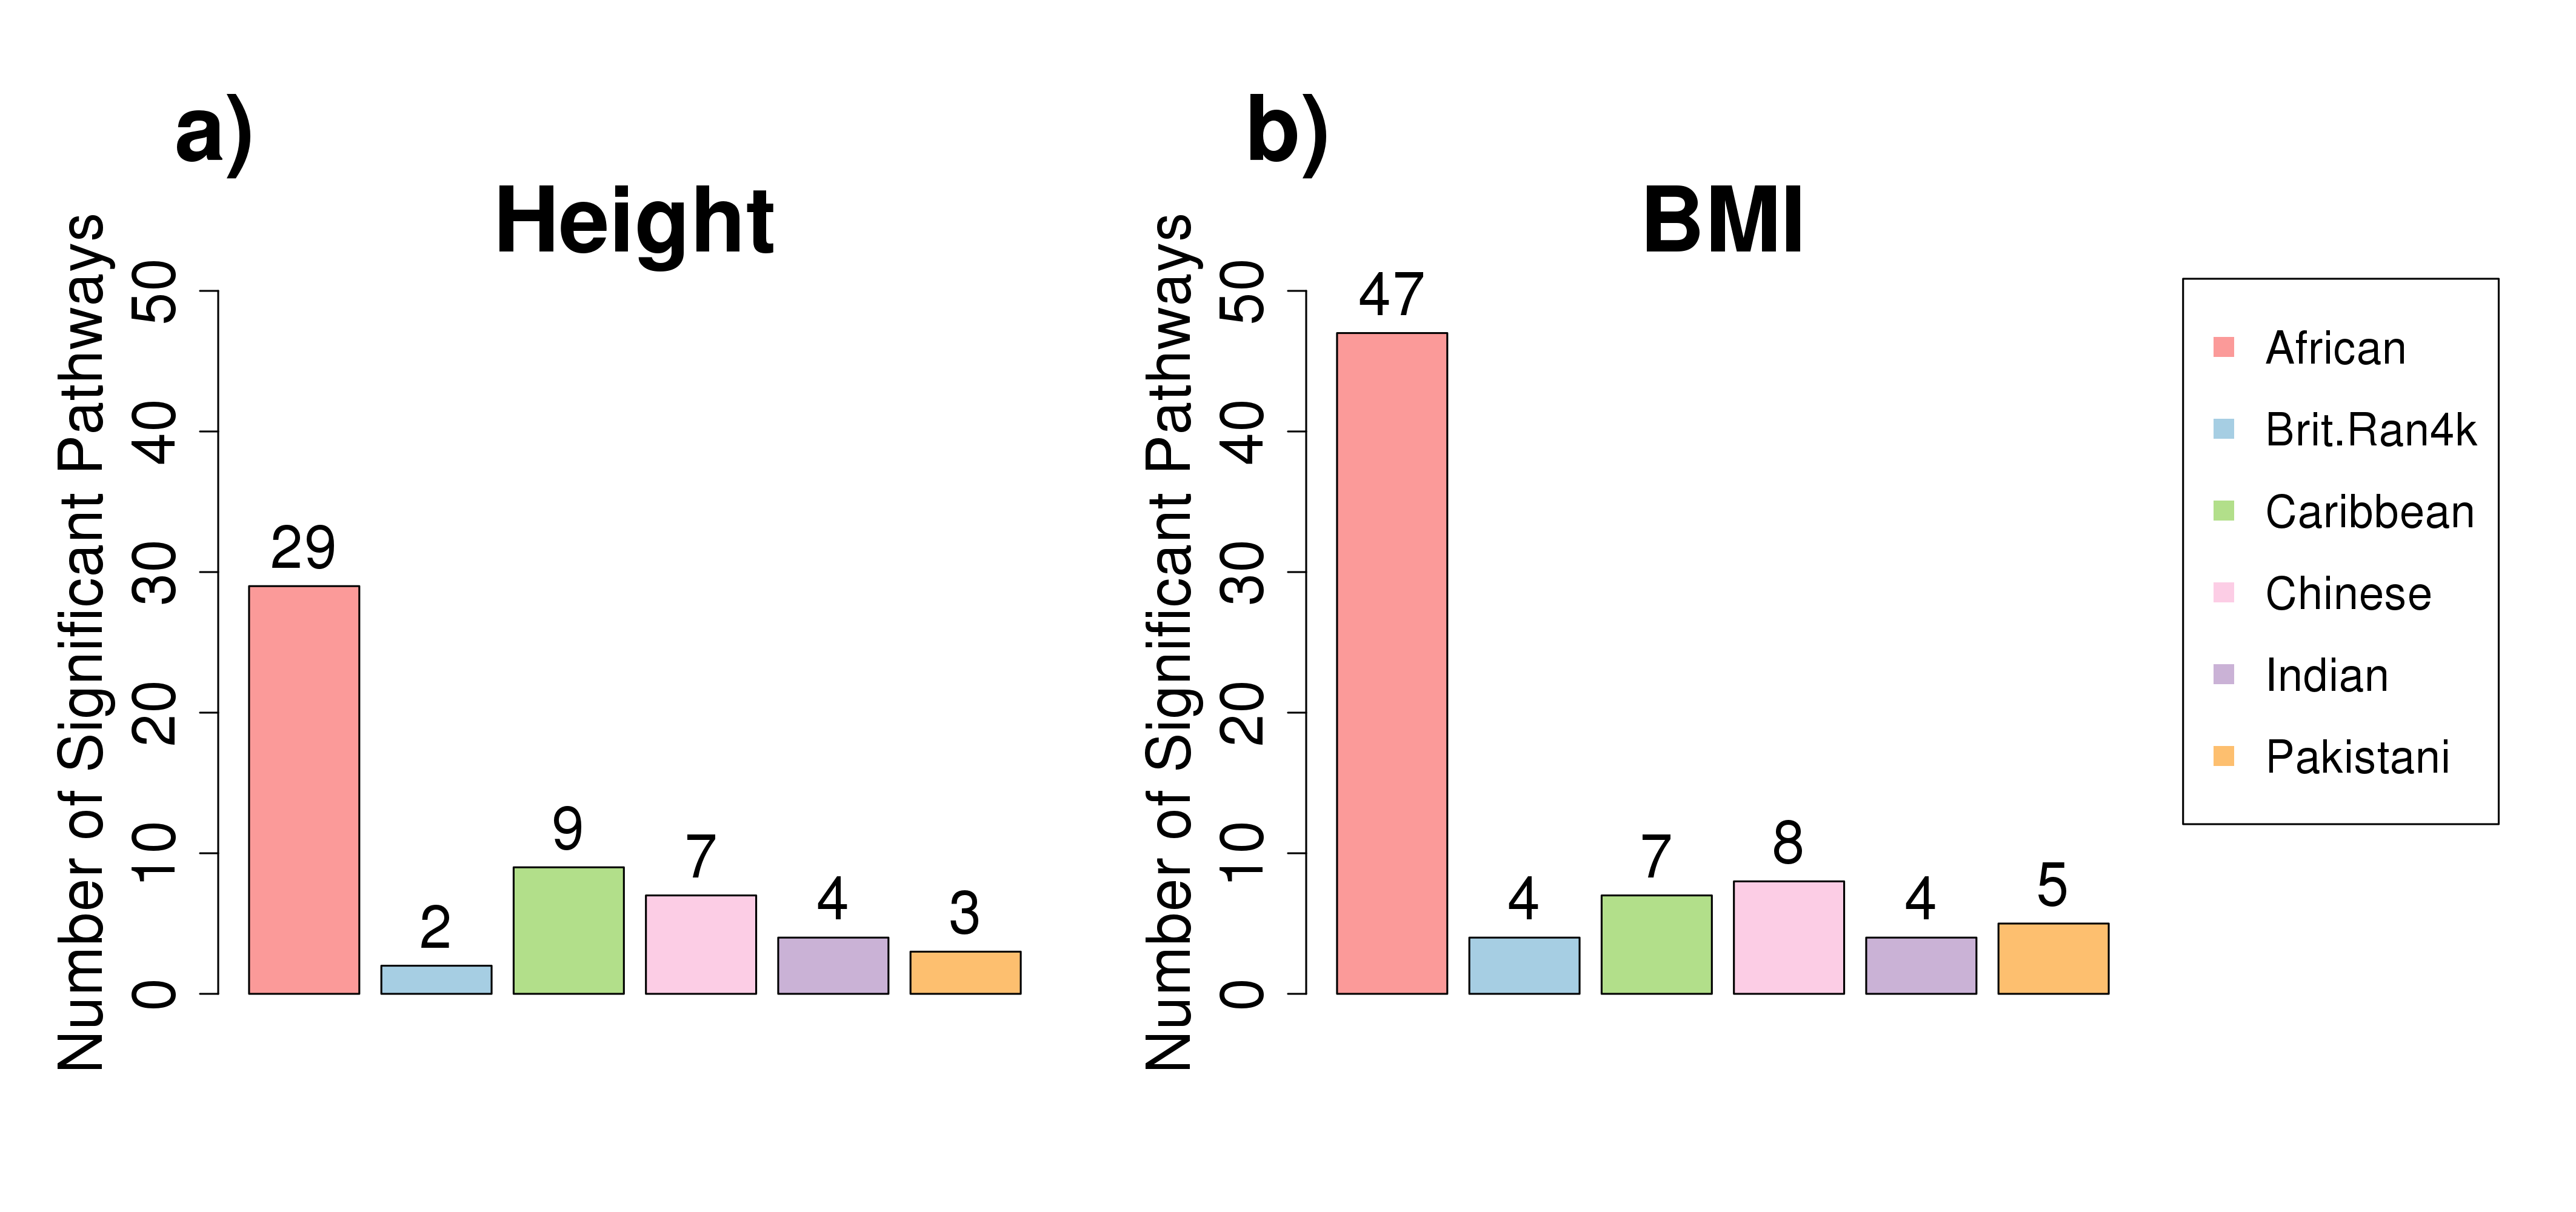
\includegraphics[scale=.45]{Images/Main/InterPath_Main_Figure_Barplots_KEGG_vs4.png}
\caption[TBD]{\textbf{Numbers of KEGG pathways that have significant marginal epistasis, per subgroup}. The figure shows the numbers of genome-wide significant pathways found from running MAPIT-R on (a) height and (b) BMI in the KEGG database within each of the UKB subgroups.  Genome-wide significance was determined by using Bonferroni-corrected $p$-value thresholds based on the number of pathways tested in each database-phenotype-subgroup combination (Supplementary Table \ref{InterPath-Supp-Table-UKBPopStats}). Across all database-phenotype combinations, the African subgroup has the largest numbers of significant pathways. For lists of the specific significant pathways per database-phenotype-subgroup combination, see Supplementary Tables \ref{InterPath-Supp-Table-TopPathways-AllPaths-AllPhenos}\textcolor{blue}{a-d}. Results from running MAPIT-R with REACTOME database pathways can be found in Supplementary Figure \ref{InterPath-Supp-Figure-Barplots-REACTOME}.}
\label{InterPath-Main-Figure-Barplots-KEGG}
\end{figure}

\begin{table}[ht]
\centering
\begin{tabular}{lrr}
  \hline
\textbf{KEGG Pathway} & \textbf{Height} & \textbf{BMI} \\ 
& \textbf{$p$-Value} & \textbf{$p$-Value} \\ 
  \hline
  \textbf{Cellular Signaling:} & & \\
 CHEMOKINE\_SIGNALING\_PATHWAY & 5.14E-10 & 1.51E-08 \\
 CYTOKINE\_CYTOKINE\_RECEPTOR\_INTERACTION & 2.84E-08 & NS \\
 WNT\_SIGNALING\_PATHWAY & 6.54E-06 & 1.41E-07 \\
 ERBB\_SIGNALING\_PATHWAY & NS & 3.30E-07 \\
  \\
  \textbf{Immune Systems:} & & \\
  AUTOIMMUNE\_THYROID\_DISEASE & 1.49E-06 & 1.39E-08 \\
  ALLOGRAFT\_REJECTION & 8.15E-06 & 2.53E-08 \\
  ANTIGEN\_PROCESSING\_AND\_PRESENTATION & 2.89E-05 & 2.08E-07 \\
  \\
  \textbf{Heart Conditions:} & & \\
  DILATED\_CARDIOMYOPATHY & 1.24E-07 & 6.99E-06 \\
  VIRAL\_MYOCARDITIS & 1.89E-05 & 1.09E-06 \\
  \\
  \textbf{Metabolism:} & & \\
  PURINE\_METABOLISM & 1.19E-07 & 2.46E-06 \\
  BETA\_ALANINE\_METABOLISM & NS & 1.12E-04 \\
  ETHER\_LIPID\_METABOLISM & NS & 1.41E-04 \\
  O\_GLYCAN\_BIOSYNTHESIS & NS & 1.92E-04 \\
   \hline
\end{tabular}
  \caption{\textbf{Biological themes among MAPIT-R significant KEGG pathways in the African subgroup}. The table shows different biological themes amongst the MAPIT-R significant pathways for both height and BMI in the African subgroup. Example pathways for each biological theme are included along with the pathway's MAPIT-R $p$-value in height and BMI. Genome-wide significance was determined by using Bonferroni-corrected $p$-value thresholds based on the number of pathways tested in each database-phenotype-subgroup combination (Supplementary Table \ref{InterPath-Supp-Table-UKBPopStats}). For a full list of MAPIT-R significant pathways in all database-phenotype-subgroup combinations, see Supplementary Tables \ref{InterPath-Supp-Table-TopPathways-AllPaths-AllPhenos}\textcolor{blue}{a-d}. `NS' indicates the pathway was not genome-wide significant for the given phenotype.}
\label{InterPath-Main-Table-KEGG-African-TopPathways-Themes}
\end{table}

The African subgroup has neither the largest sample size nor the largest number of SNPs passing QC filters, yet has the most significant epistatic signals of any subgroup analyzed  (Supplementary Table \ref{InterPath-Supp-Table-UKBPopStats}). To investigate the performance of MAPIT-R, we conducted simulation studies under a range of genetic architectures that explore different proportions of epistatic effects, and we find that MAPIT-R both controls type 1 error accurately and has power to detect pathway level marginal epistasis (Supplementary Figure XX). We also ran versions of MAPIT-R using permuted phenotypes and further find that MAPIT-R operates appropriately when epistasis is absent between any pathway and the rest of the genome (Supplementary Figures \ref{InterPath-Supp-Figure-perm1-QQPlots-AllPaths} and \ref{InterPath-Supp-Figure-10perms-pValHists}); these permutations allow us to investigate MAPIT-R's false discovery rates and we observe values only as high as 1.5\% across our different database-phenotype-subgroup combinations at multiple significance thresholds (Supplementary Table \ref{InterPath-Supp-Table-AllPops-FDRs}).

\subsection{Non-African subgroups reveal additional pathways with significant marginal epistasis}

In our analyses of the British, Chinese, Caribbean, Indian, and Pakistani subgroups, we identify 80 pathways in total that have significant marginal epistatic interactions across the different database-phenotype combinations. Many of these other pathways overlap with the set of significant results from the African subgroup, though there is less overlap among other non-African subgroups (Figure \ref{InterPath-Main-Figure-Barplots-KEGG}\& Supplementary Figure \ref{InterPath-Supp-Figure-Heatplots-REACTOME}). For example, in the KEGG-height analysis, six of the seven pathways with significant marginal epistasis identified using the Caribbean subgroup overlap with those identified using the African subgroup, and seven of the eight pathways with significant marginal epistasis identified using the Chinese subgroup overlap with those identified using the African subgroup. However, there is no overlap in results from our marginal epistasis scans at the pathway level between the Chinese and Caribbean subgroups.

\begin{figure}[htb]
\centering
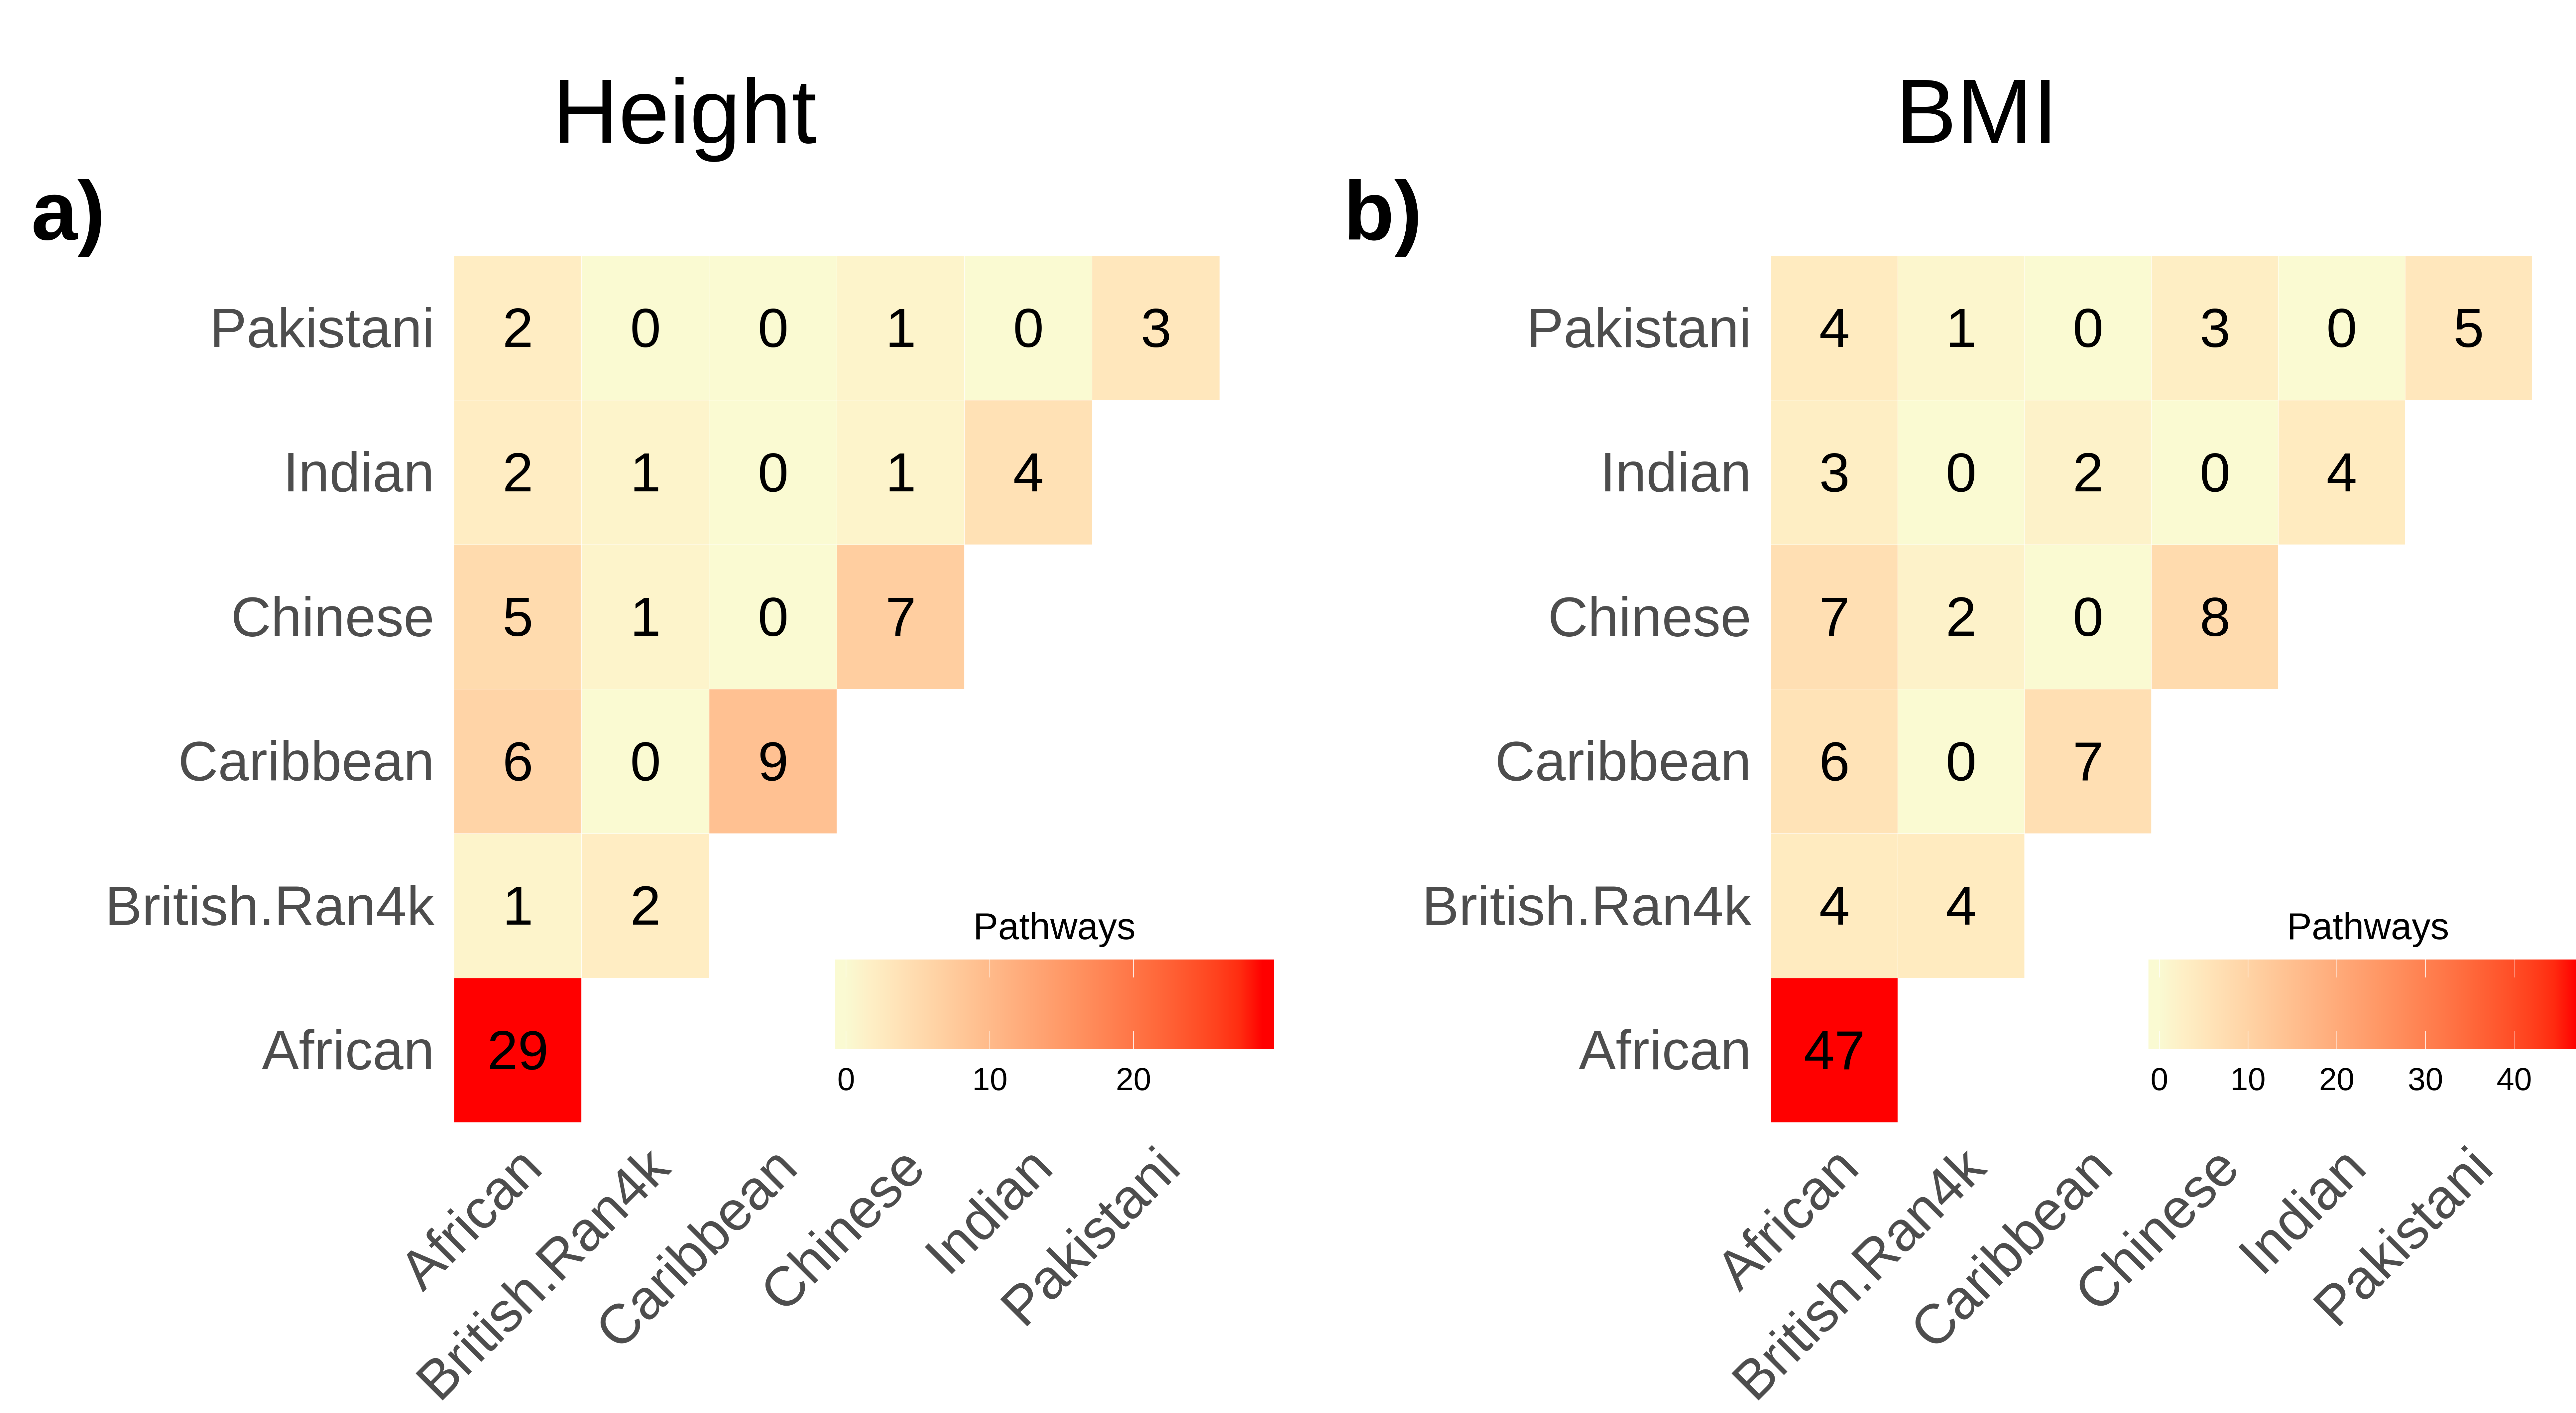
\includegraphics[scale=.225]{Images/Main/InterPath_Main_Figure_Heatplots_KEGG_vs4.png}
\caption[TBD]{\textbf{Overlap of MAPIT-R significant KEGG pathways between UKB subgroups}. The heatplots show the numbers of genome-wide significant MAPIT-R pathways that overlap between each UKB subgroup for (a) height and (b) BMI in the KEGG database. Results for both phenotypes in the REACTOME database can be seen in Supplementary Figure \ref{InterPath-Supp-Figure-Heatplots-REACTOME}. The diagonal shows the total number of genome-wide significant pathways per population subgroup. We observe that significant pathways observed in non-African subgroups overlap more often with pathways from the African subgroup than they do with pathways from the other, remaining non-African subgroups.}
\label{InterPath-Main-Figure-Heatplots-KEGG}
\end{figure}

The pathways with significant marginal epistasis identified in both the African and Caribbean subgroups are related to the cellular signaling and heart condition patterns; the genes in these overlapping pathways include multiple kinases (e.g, {\emph{MAPK1}}, {\emph{ROCK1}}, {\emph{PRKCB}}, {\emph{PAK1}}) and calcium channel proteins (e.g., {\emph{CACNA1S}}, {\emph{CACNA1D}}) (Supplementary Tables \ref{InterPath-Supp-Table-MAPITR-TopPathway-Overlap} \& \ref{InterPath-Supp-Table-MAPITR-TopPathway-GeneCounts-Overlap}). In contrast, the pathways with significant marginal epistasis identified in both the African and Chinese subgroups are pathways related to the immune system and contain multiple HLA loci (e.g., {\emph{HLA-DRA}}, {\emph{HLA-DRB1}}, {\emph{HLA-A}}, {\emph{HLA-B}})  (Supplementary Tables \ref{InterPath-Supp-Table-MAPITR-TopPathway-Overlap} \& \ref{InterPath-Supp-Table-MAPITR-TopPathway-GeneCounts-Overlap}). Recent work has also suggested that Han Chinese may be particularly enriched for interactions involving HLA loci \citep{Deng2020}. 

\subsection{Stronger signals of pathway-level marginal epistasis underlie BMI than height}

In our analyses of marginal epistasis at the pathway-level in the African subgroup, we find that BMI contains more significant pathways than does height, in both the KEGG and REACTOME databases (Figure \ref{InterPath-Main-Figure-Barplots-KEGG} and Supplementary Figure \ref{InterPath-Supp-Figure-Barplots-REACTOME}). While there is a strong correlation between height and BMI MAPIT-R -$\log_{10}$ $p$-values (.758 in KEGG and .716 in REACTOME), there are consistently more pathways with significant marginal epistasis signals in BMI (Figure \ref{InterPath-Main-Figure-MAPITR-PhenoComps-African}). These results align with pedigree-based heritability estimates for each trait, which have indicated narrow-sense heritability is around 0.8 in height and between 0.4 and 0.6 in BMI \citep{Elks2012,Visscher2012}. Taken together, these estimates suggest that non-additive effects may play a greater role in BMI than height, as observed here. 

\begin{figure}[htb]
\centering
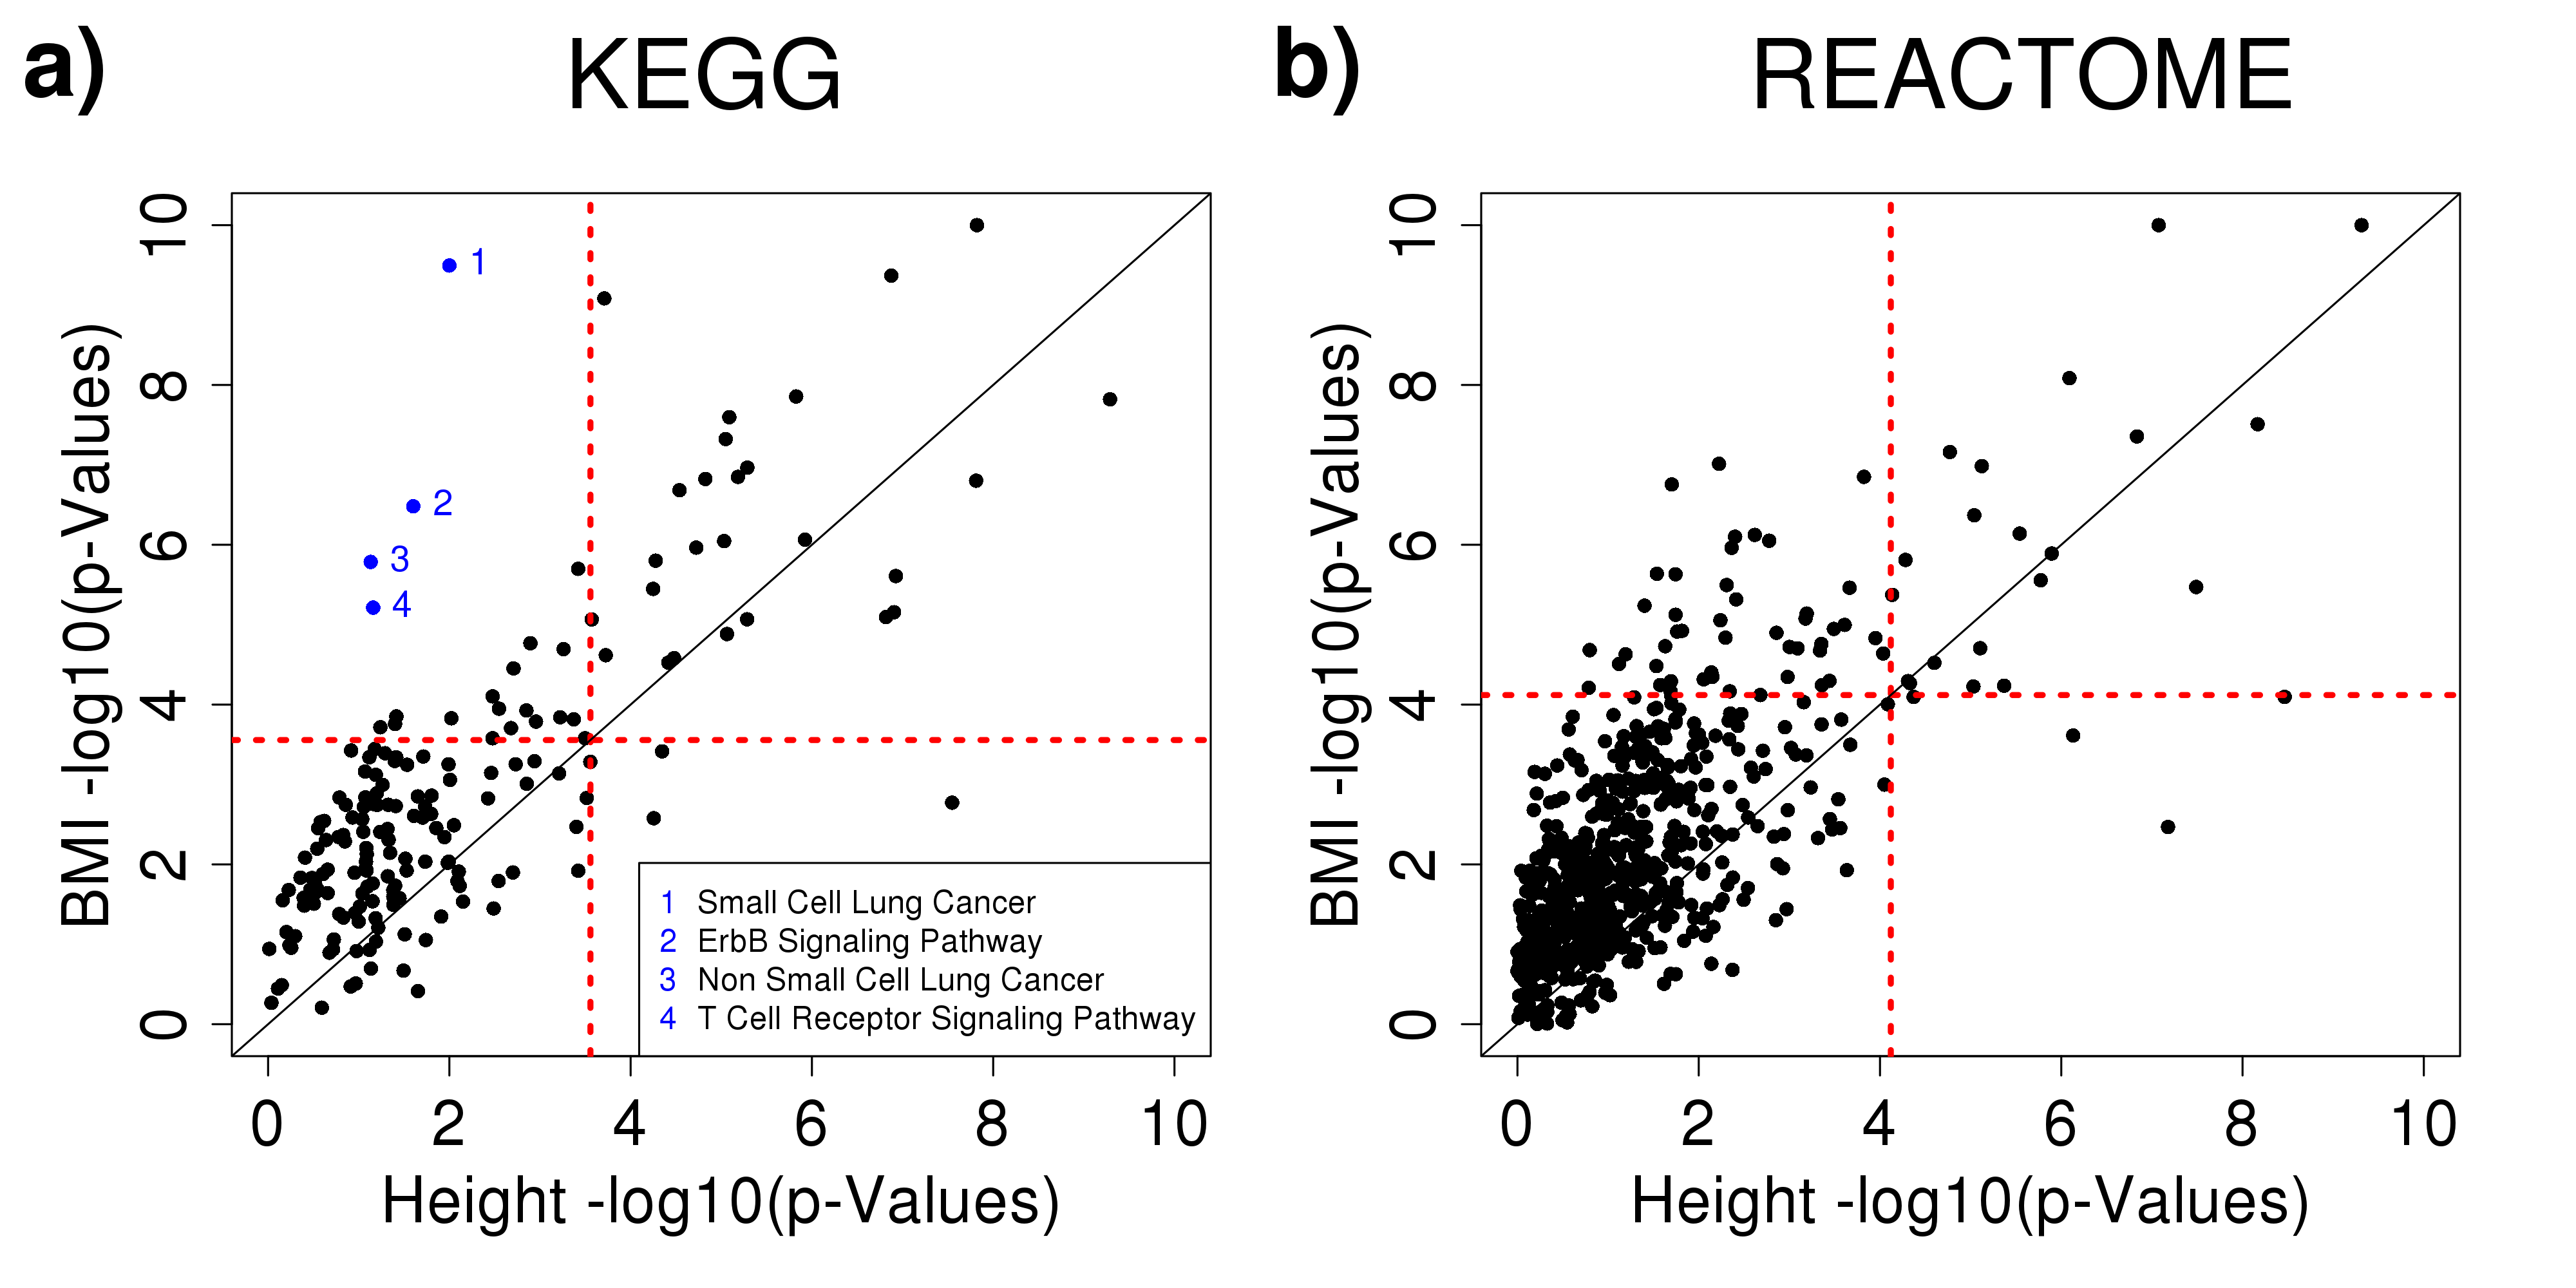
\includegraphics[scale=.45]{Images/Main/InterPath_Main_Figure_MAPITR_PhenoComps_African_vs4_legend.png}
\caption[TBD]{\textbf{Comparison of BMI vs. height MAPIT-R results in the African subgroup}. The figure shows MAPIT-R BMI results plotted against MAPIT-R height results for all pathways from the (a) KEGG and (b) REACTOME databases in the African subgroup. The $x$-axis is the MAPIT-R height -$\log_{10}$ $p$-value and the $y$-axis is the MAPIT-R BMI -$\log_{10}$ $p$-value. The dotted red lines are the Bonferroni-corrected $p$-value thresholds for genome-wide significance in each pathway-phenotype combination (Supplementary Table \ref{InterPath-Supp-Table-UKBPopStats}). The four highlighted pathways in blue represent a cluster that have more significant $p$-values in BMI than height. Across both databases, BMI results have lower MAPIT-R $p$-values than height results on average. For these comparisons in all the UKB subgroups, see Supplementary Figure \ref{InterPath-Supp-Figure-MAPITR-PhenoComps-AllPops}.}
\label{InterPath-Main-Figure-MAPITR-PhenoComps-African}
\end{figure}

We detect one cluster of pathways in the KEGG results  with divergent statistical evidence for marginal epistasis in height versus BMI (Figure \ref{InterPath-Main-Figure-MAPITR-PhenoComps-African}). The four highlighted pathways in Figure \ref{InterPath-Main-Figure-MAPITR-PhenoComps-African} are signaling and oncogenic pathways: sorted by increasing $p$-value, these are Small Cell Lung Cancer ($p$-value: 3.20E-10), ErbB Signaling Pathway ($p$-value: 3.30E-07), Non Small Cell Lung Cancer ($p$-value: 1.64E-06), and T Cell Receptor Signaling Pathway ($p$-value: 6.12E-06). Two sets of gene families appear in all four of these pathways: (Supplementary Table \ref{InterPath-Supp-Table-MAPITR-PhenoComps-African-GeneCounts}): phosphatidylinositol 3-kinases (PIKs) and the AKT serine/threonine-protein kinases. One gene in this group, \emph{AKT2}, has been associated with multiple monogenic disorders of glucose metabolism, including severe insulin resistance and diabetes, and severe fasting hypoinsulinemic hypoglycemia \citep{George2004,Manning2017,Latva-Rasku2018}, representing a possible driver of this cluster. Additionally, we observe multiple oncogenic pathways among top epistatic signals, and other recent work suggests epistasis may be an important feature of cancer \citep{Wang2014,Jamshidi2015,Fang2019,Li2019,Ma2019}. 

\subsection{Testing variability in MAPIT-R results with British replicate subpopulations}

One important consideration of our results is that the diverse non-European human ancestries we are analyzing have smaller sample sizes than do recent GWA studies in individuals of European ancestry. Given the large sample size of the white British individuals in the UK BioBank, we decided to test whether the subsampled subgroup of this cohort---if similar in size to the sample sizes of non-European ancestry cohorts in the UK Biobank---would be large enough to be representative of the genetic variation in the full white British sample of over 470,000 individuals. Specifically, we sampled four additional, non-overlapping random subgroups of 4,000 British individuals and tested whether MAPIT-R scans in those random samples were consistent with our results for the original British 4,000 subgroup.  We also constructed larger non-overlapping British subsamples of 10,000 individuals to investigate how our results might vary with sample size. In total we analyzed five non-overlapping sets of 4,000 British individuals and five non-overlapping sets of 10,000 British individuals. 

When applying MAPIT-R to these replicates of 4,000 and 10,000 white British individuals, we find that our results are similar to what was observed in the original British 4,000 subgroup (Figures \ref{InterPath-Main-Figure-Barplots-KEGG}-\ref{InterPath-Main-Figure-Heatplots-KEGG}): limited numbers of significant pathways across all database-phenotype-replicate subgroup combinations, as well as limited overlap of significant pathways between replicates (Supplementary Figures \ref{InterPath-Supp-Figure-BritReps-Barplots}\textcolor{blue}{-}\ref{InterPath-Supp-Figure-BritReps-10perms-pValHists-pt1}). We also ran analyses with permuted phenotypes to once again test the null model of no marginal epistasis between pathways and the rest of the genome, and once more we find very low FDRs (Supplementary Tables \ref{InterPath-Supp-Table-BritReps-FDRs-pt1}). Within the British subgroups then, there appears to be consistency across these random samples despite their lower sample sizes compared to full cohort of over 470,000 individuals.

\subsection{Identifying drivers of  pathway-level marginal epistatic signals}

We were also interested in identifying which genomic regions were driving pathway-level significant signals of epistasis with the rest of the genome in our MAPIT-R analyses. To explore this, we first wanted to identify whether there were any genes or gene families that appeared to be particularly enriched amongst our significant MAPIT-R pathways. We then wanted to test whether such genes or gene families were drivers of the original MAPIT-R pathway-level signals. To accomplish this first part, we conducted two types of hypergeometric tests for enrichment to identify genes that were significantly overrepresented amongst the pathways that showed significant marginal epistatic interactions with the rest of the genome (Supplementary Tables \ref{InterPath-Supp-Table-TopPathways-AllPaths-AllPhenos}\textcolor{blue}{a-d}). 

First, we conducted a standard hypergeometric test for enrichment by comparing the number of times a gene appears amongst the set of significant MAPIT-R pathways for a given UKB pathway database-phenotype-subgroup combination against the number of times that same gene appears amongst the set of all pathways for the same pathway database (KEGG or REACTOME). However, this test may be confounded by the fact that larger pathways have more SNPs and are therefore more likely to have significant MAPIT-R $p$-values (see Supplementary Figure \ref{InterPath-Supp-Figure-pValsVsNumSNPs}). As a second approach, we also ran tests for enrichment using only MAPIT-R significant pathways that were also below a specific size threshold; by focusing on smaller pathways, we could assess the extent to which pathway size may confound our gene enrichment tests. 

\begin{figure}[htbp]
\centering
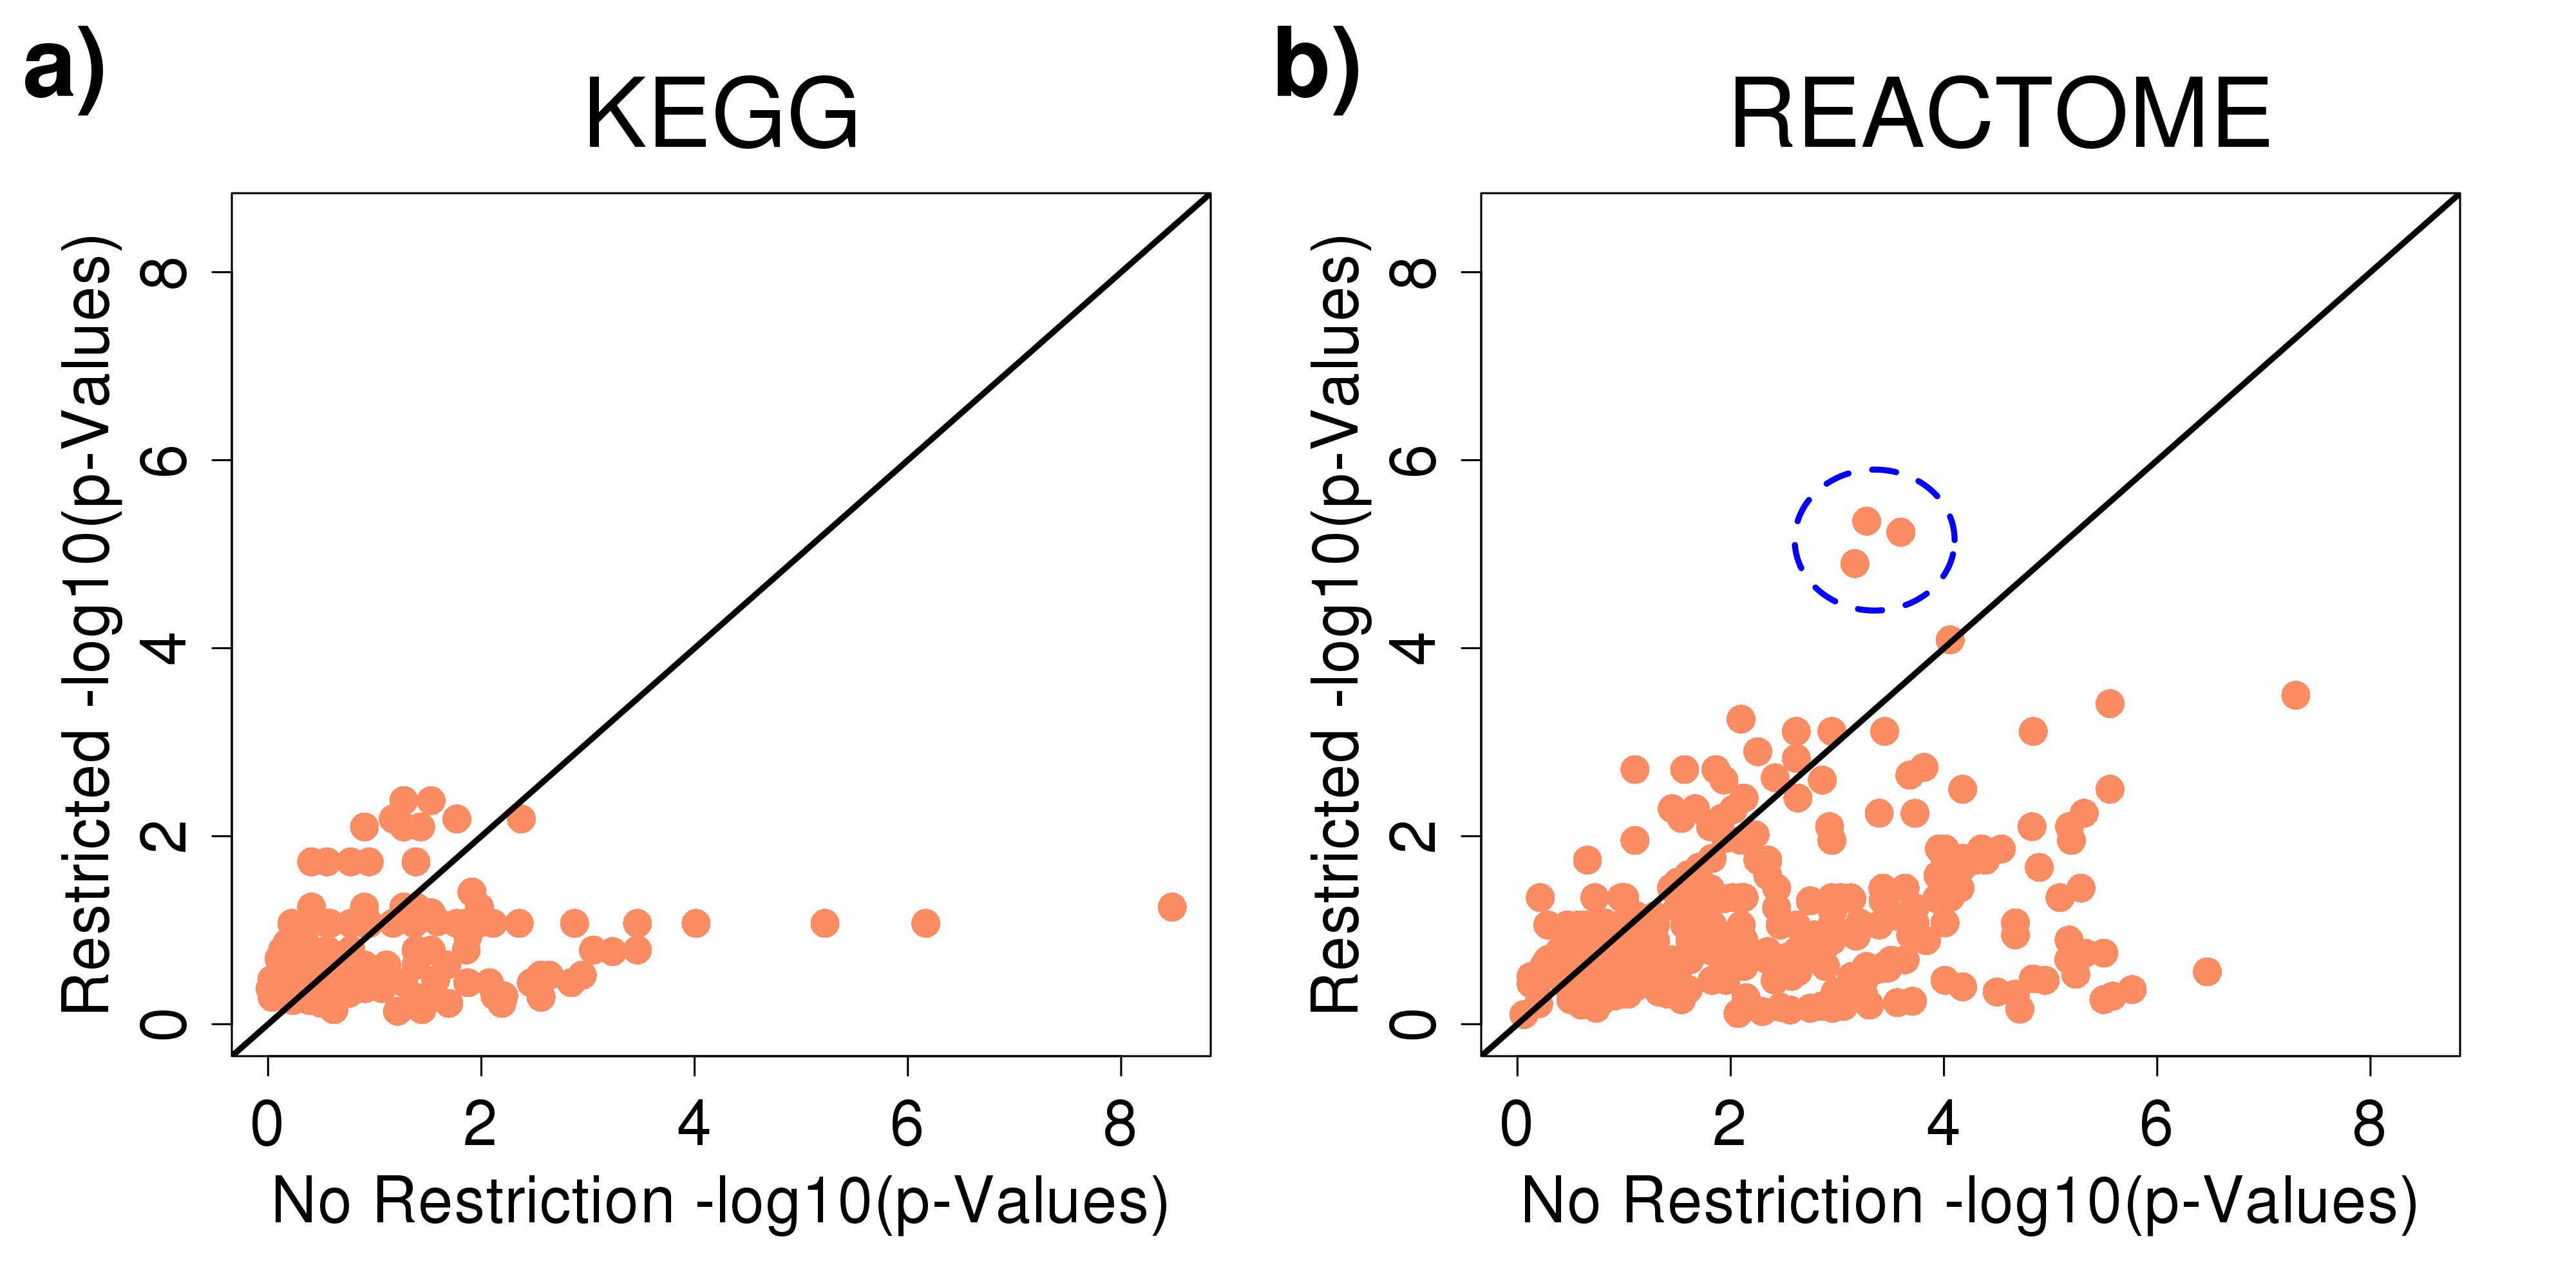
\includegraphics[scale=.4]{Images/Main/InterPath_Main_Figure_Hypergeometric_RestrictedComps_African_BMI_vs4.png}
\caption[TBD]{\textbf{Comparison of gene count hypergeometric enrichment $p$-values in BMI using pathway size of at most 1000 SNPs versus no size restrictions in the African subgroup}. The figure shows comparisons of the gene-based hypergeometric enrichment $p$-values between the size restricted version of the analysis and the original unrestricted version of the analysis in the (a) KEGG and (b) REACTOME pathway databases. Only results for BMI are shown because few MAPIT-R significant pathways in the height analysis remained after the size restriction step. The $x$-axis shows the original, unrestricted hypergeometric -$\log_{10}$ $p$-values, and the $y$-axis shows the new, size restricted hypergeometric -$\log_{10}$ $p$-values. The proteasome gene family cluster is highlighted (blue dashed circle) in the REACTOME plot. For lists containing each gene's original and  size-restricted hypergeometric $p$-values, see Supplementary Table \ref{InterPath-Supp-Table-Hypergeometric-RestrictedComps-African-BMI}.}
\label{InterPath-Main-Figure-Hypergeometric-RestrictedComps-African-BMI}
\end{figure}
\clearpage

Figure \ref{InterPath-Main-Figure-Hypergeometric-RestrictedComps-African-BMI} shows, for each gene in a MAPIT-R significant pathway, its
 hypergeometric $p$-value from both analyses; we also highlight genes that decreased their $p$-value (that is, that increased the strength of their enrichment $p$-value) in the  enrichment analysis restricted to smaller pathways compared to the full analysis with all significant pathways in that database-phenotype-cohort analysis. We focused on the MAPIT-R test combination of REACTOME-BMI-African subgroup since no other subgroup contained enough remaining significant pathways after restricting to smaller pathways (see Materials and Methods).  These genes and gene families are all from the same protein complex (shown in circle in Figure \ref{InterPath-Main-Figure-Hypergeometric-RestrictedComps-African-BMI}\textcolor{blue}{b}), the proteasome ({\emph{PSMA}}, {\emph{PSMB}}, {\emph{PSMC}}, {\emph{PSMD}}, {\emph{PSME}}, and {\emph{PSMF}}). The proteasome is one half of the ubiquitin-proteasome system (UPS), a critical system for a variety of processes related to protein degradation within the cell \citep{Voges1999,Livneh2016,Collins2017}. Whereas ubiquitin is the first half of this system that tags proteins for eventual degradation, the proteasome is the second half of this system that catalyzes the degradation itself. The main proteasome isoform, 26S, is made up of two main components: the 20S core particle (CP) of four stacked rings (two outer, structural rings encoded by \emph{PSMA} genes, and two inner, catalytic rings encoded by \emph{PSMB} genes) and the 19S regulatory particle (RP) which caps both ends of the CP (encoded by both \emph{PSMC} and \emph{PSMD} genes) (Figure \ref{InterPath-Main-Figure-Proteasome-Panels}\textcolor{blue}{a}). Since these gene families covered both a large number of genomic sites as well as known biological functions, we used the proteasome as a test case to further explore refining MAPIT-R pathway-level signals.

\begin{figure}[htbp]
\centering
\hspace*{-2.5cm}
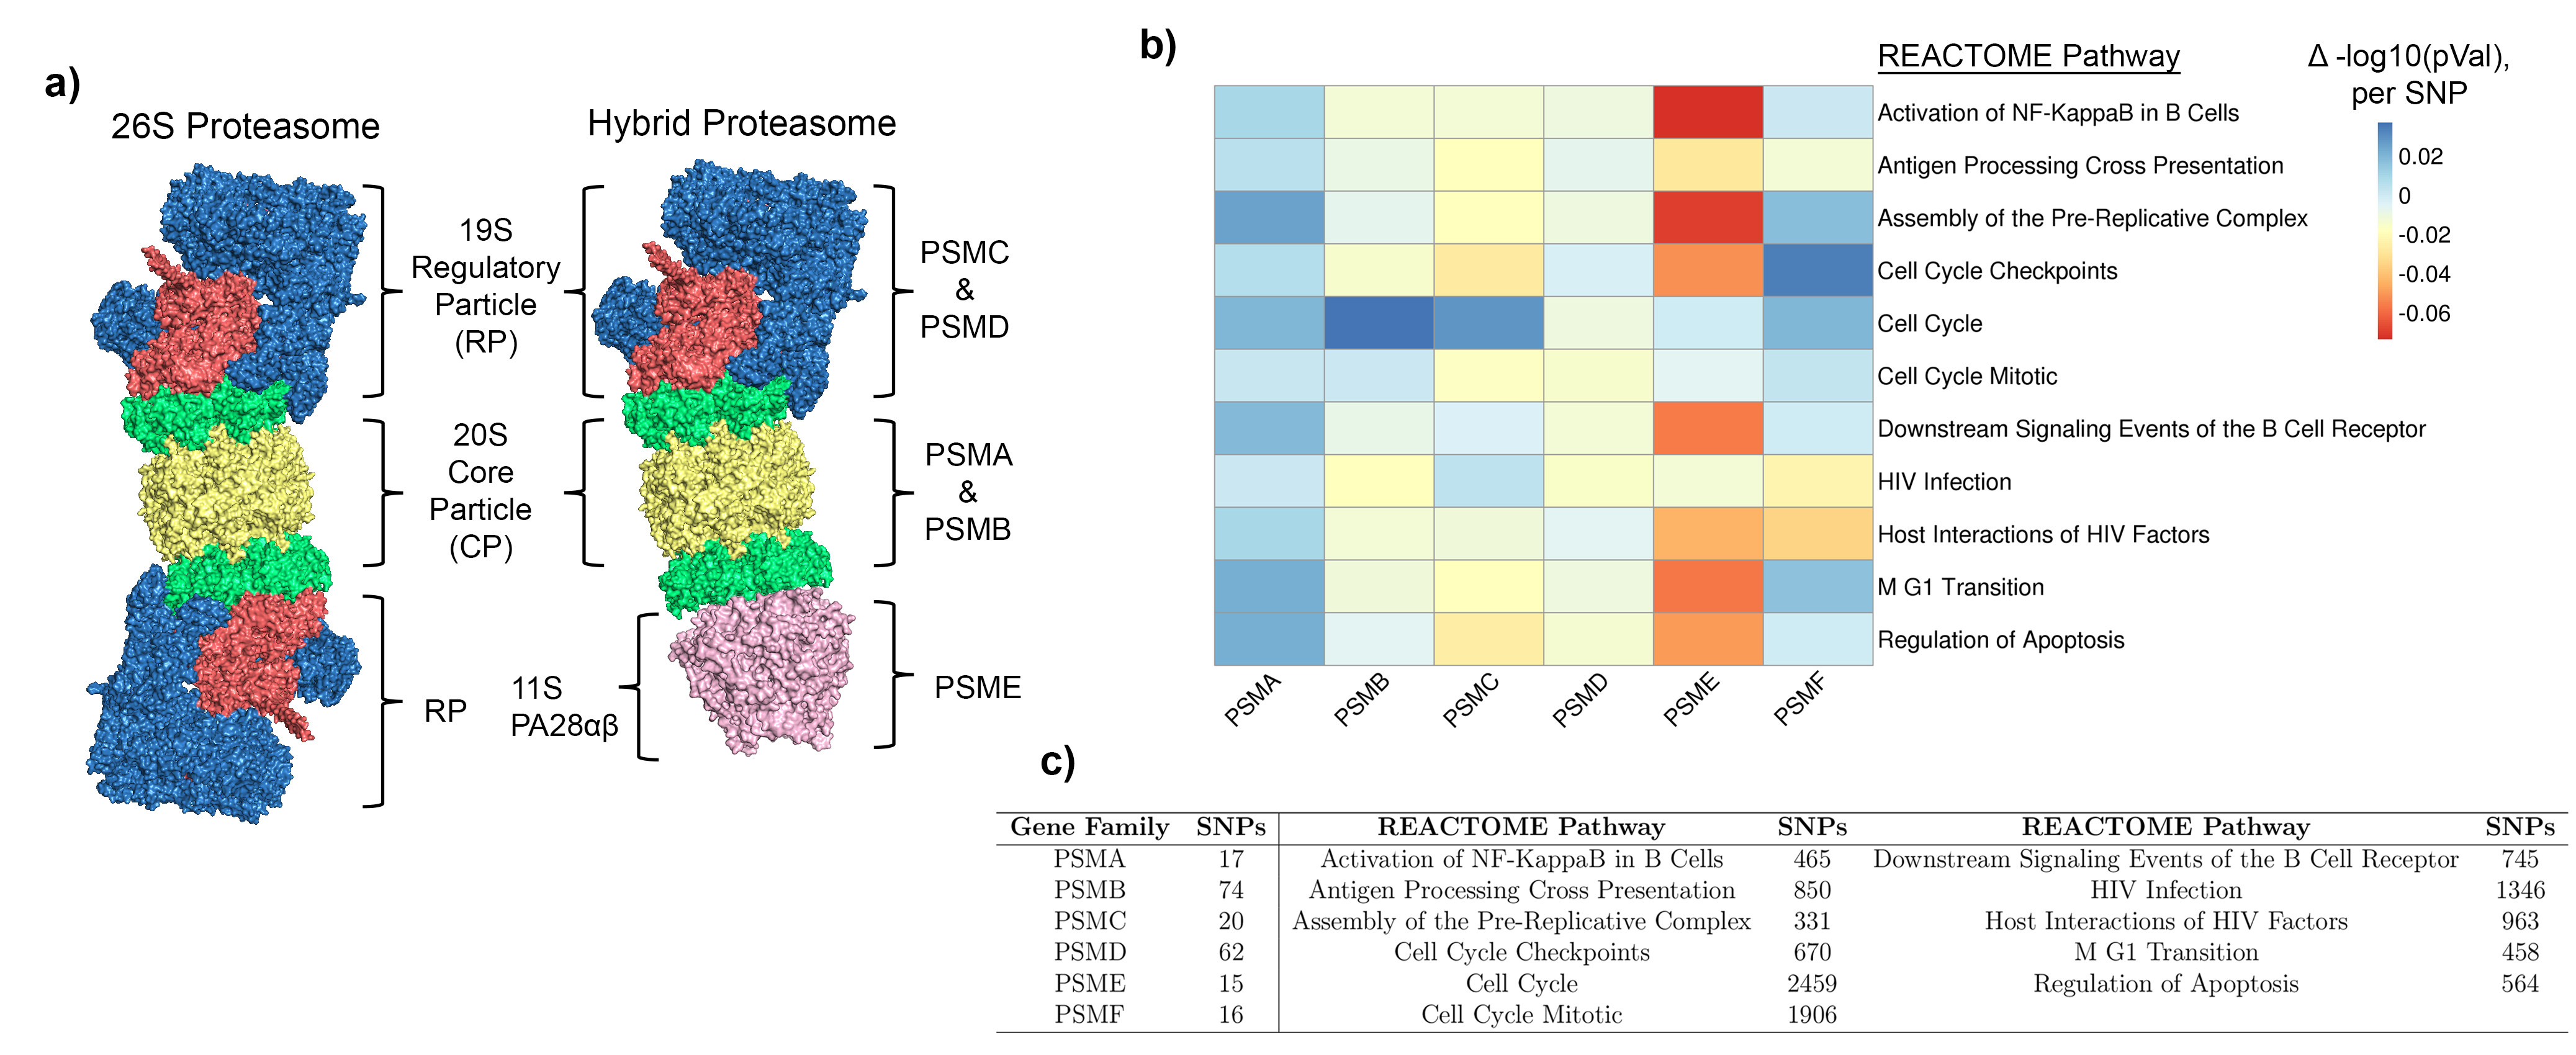
\includegraphics[scale=.55]{Images/Main/InterPath_Main_Figure_Proteasome_vs2.png}
\caption[TBD]{\textbf{Structure of the proteasome and results from applying a `leave-one-out' approach to MAPIT-R with proteasome gene families}. \textbf{(a)} The figures show models of different isoforms of the proteasome. The `26S Proteasome' is the main isoform, composed of the 20S core particle (CP) and capped on both ends by  the 19S regulatory particle (RP), which is required for degradation of ubiquitinated proteins. The `Hybrid Proteasome' isoform is produced when the CP binds on one end with a RP and on the other end with the IFN-$\gamma$-inducible complex PA28$\alpha\beta$. The \textit{PSMA} and \textit{PSMB} gene families encode the proteins for the CP, the \textit{PSMC} and \textit{PSMD} gene families encode the proteins for the RP, and the \textit{PSME} gene family encodes PA28$\alpha\beta$. Note that \textit{PSMF} represents a proteasome inhibitor and is not shown. The structures shown were adopted and modified from the Protein Data Bank (human 26S proteasome, \href{https://www.rcsb.org/structure/5GJR}{5GJR}; mouse PA28$\alpha\beta$, \href{https://www.rcsb.org/structure/5MX5}{5MX5}) and from \citet{Murata2018}. \textbf{(b)} The heatplot shows the change in original MAPIT-R -$\log_{10}$ $p$-value for each presented REACTOME pathway when each proteasome gene family is removed one at a time in a `leave-one-out' manner. The analyses were conducted in the BMI-African subgroup combination. The $x$-axis shows each proteasome gene family and the $y$-axis shows each REACTOME pathway. Each column has been scaled by the number of SNPs present in the given gene families and, as a result, the heatplot specifically shows the -$\log_{10}$ $p$-value change per SNP. \textbf{(c)} The table shows the number of SNPs present in each proteasome gene family (left), as well as the number of SNPs present in each REACTOME pathway (right).}
\label{InterPath-Main-Figure-Proteasome-Panels}
\end{figure}

To further investigate whether the proteasome drives pathway-level signals of marginal epistasis, we first collected all the significant MAPIT-R pathways from the REACTOME-BMI-African analysis that contained every proteasome gene family. Next we identified whether any of these individual gene families ({\emph{PSMA}}, {\emph{PSMB}}, {\emph{PSMC}}, {\emph{PSMD}}, {\emph{PSME}}, and {\emph{PSMF}}) had particularly strong effects on the original MAPIT-R $p$-values. To accomplish this, we removed each gene family one at a time from the original significant pathways and then conducted MAPIT-R analyses using these `one-gene-family-removed' pathways; we then compared these new MAPIT-R $p$-values to each pathway's original, full MAPIT-R $p$-value and identified whether the removal of any particular gene families lead to large changes across multiple pathways.  

Figure \ref{InterPath-Main-Figure-Proteasome-Panels}\textcolor{blue}{b} shows the results from this analysis, where we find that the \emph{PSMA} and \emph{PSME} gene families have potentially biologically interpretable patterns of $p$-value changes across multiple REACTOME pathways. For the \emph{PSMA} gene family, we observe almost no examples of where removing these genes leads to an increase in the MAPIT-R $p$-value. The \emph{PSMA} gene family encodes the outer two rings of the core four rings in the main 20S core. These outer, `alpha' rings are gates which control the entry of proteins into the core of the proteasome. Unlike the regulatory caps or the inner `beta' rings encoded by the \emph{PSMB} family, which contain protease active sites, the outer rings have no known major catalytic functionality. This lack of catalytic activity then may explain the lack of increase in MAPIT-R $p$-values, or lack of information lost, when \emph{PSMA} genes are removed from analysis. For the the \emph{PSME} gene family, we find some of the largest increases in MAPIT-R $p$-values across multiple REACTOME pathways. The \emph{PSME} gene family encodes an alternative regulatory particle, 11S PA28$\alpha\beta$, that can also associate with the 20S core; these alternative isoforms, which can contain either two 11S caps or one 11S and one 19S cap (a `hybrid proteasome'), are part of a subset of proteasomes known as immunoproteasomes. Immunoproteasomes are specialized isoforms that are expressed at higher levels in hematopoietic cells and are more directly associated with immunity-related processes such as MHC antigen presentation \citep{Ferrington2012,Basler2013,McCarthy2015}. PA28$\alpha\beta$ itself is an Interferon-$\gamma$ (IFN-$\gamma$) inducible regulatory protein that operates in a ubiquitin-independent manner and increases production of a specific subset of MHC-1 presenting antigens \citep{Groettrup1996,de2011,Raule2014,Murata2018}. Additionally, recent work has more directly connected \emph{PSME} genes as potential upregulators of NF$\kappa$B \citep{Sun2016,Mitchell2019}. Therefore these connections to immune activity may explain why removal of the \emph{PSME} gene family affects pathways related to NF$\kappa$B, B cells, HIV, and apoptosis more than other proteasome gene families. Lastly, conducting these `leave-one-out' MAPIT-R analyses in the other remaining UKB subgroups, we observe that removing the \emph{PSME} gene family often leads to some of the largest increases in MAPIT-R $p$-values across all of the gene family and REACTOME pathways combinations analyzed; this is consistent with our results of \emph{PSME} being potentially important to proteasome epistatic interactions with the rest of the genome (Supplementary Figures \ref{InterPath-Supp-Figure-Prot-Heatplots-African}-\textcolor{blue}{f}). 

\subsection{Investigating the relationship between subgroup genetic variation and signals of marginal epistasis}

MAPIT-R analyses of the African subgroup in the UKB produced the majority of significant MAPIT-R results, but why is there such a difference in significant pathways between the African subgroup and the rest of the subgroups we analyzed? One possibility may be related to heterogeneity in population structure among the UKB subgroups. We observed in our analyses that the African subgroup had much larger eigenvalue proportions of variance explained (PVE) among the top 10 local principal components from the earlier PCA (Figure \ref{InterPath-Main-Figure-Eigenvalues}). As Figure \ref{InterPath-Main-Figure-Eigenvalues} displays, we in fact observe an ordering of our subgroups on PC1 that relatively matches the ordering of which subgroups have the most significant MAPIT-R pathways. Perhaps what is driving this large number of results in the African subgroup then is a greater ability to capture and remove population structure than compared to the other subgroups. Epistatic signals tend to be more subtle, so being able to remove a larger proportion of unrelated background noise might lead to more effective identification of epistatic signals. 

To investigate this hypothesis, we tested whether pathways that covered greater proportions of the genome that were `highly loaded' on PC1 lead to more significant MAPIT-R $p$-values. Here, we define a genomic region as being `highly loaded' on PC1 if it contains any SNP that exists in the 2.5\% tails of the PC1 SNP loading score distributions for a given subgroup (see Materials and Methods). Therefore, we calculated the proportion of SNPs for each pathway that fall in these PC1 loading score tails, and compared these proportions against each pathway's MAPIT-R $p$-value. As (Supplementary) Figure \ref{InterPath-Supp-Figure-PC1Loading-AllPaths} shows however, we find no significant relationship between a pathway's proportion of SNPs that are `highly loaded' on PC1 and that pathway's MAPIT-R $p$-value. This lack of a relationship may be a result of our limited sample sizes or indicative that there is no connection between MAPIT-R results and cryptic population structure as represented by principal component space.

\begin{figure}[htb]
\centering
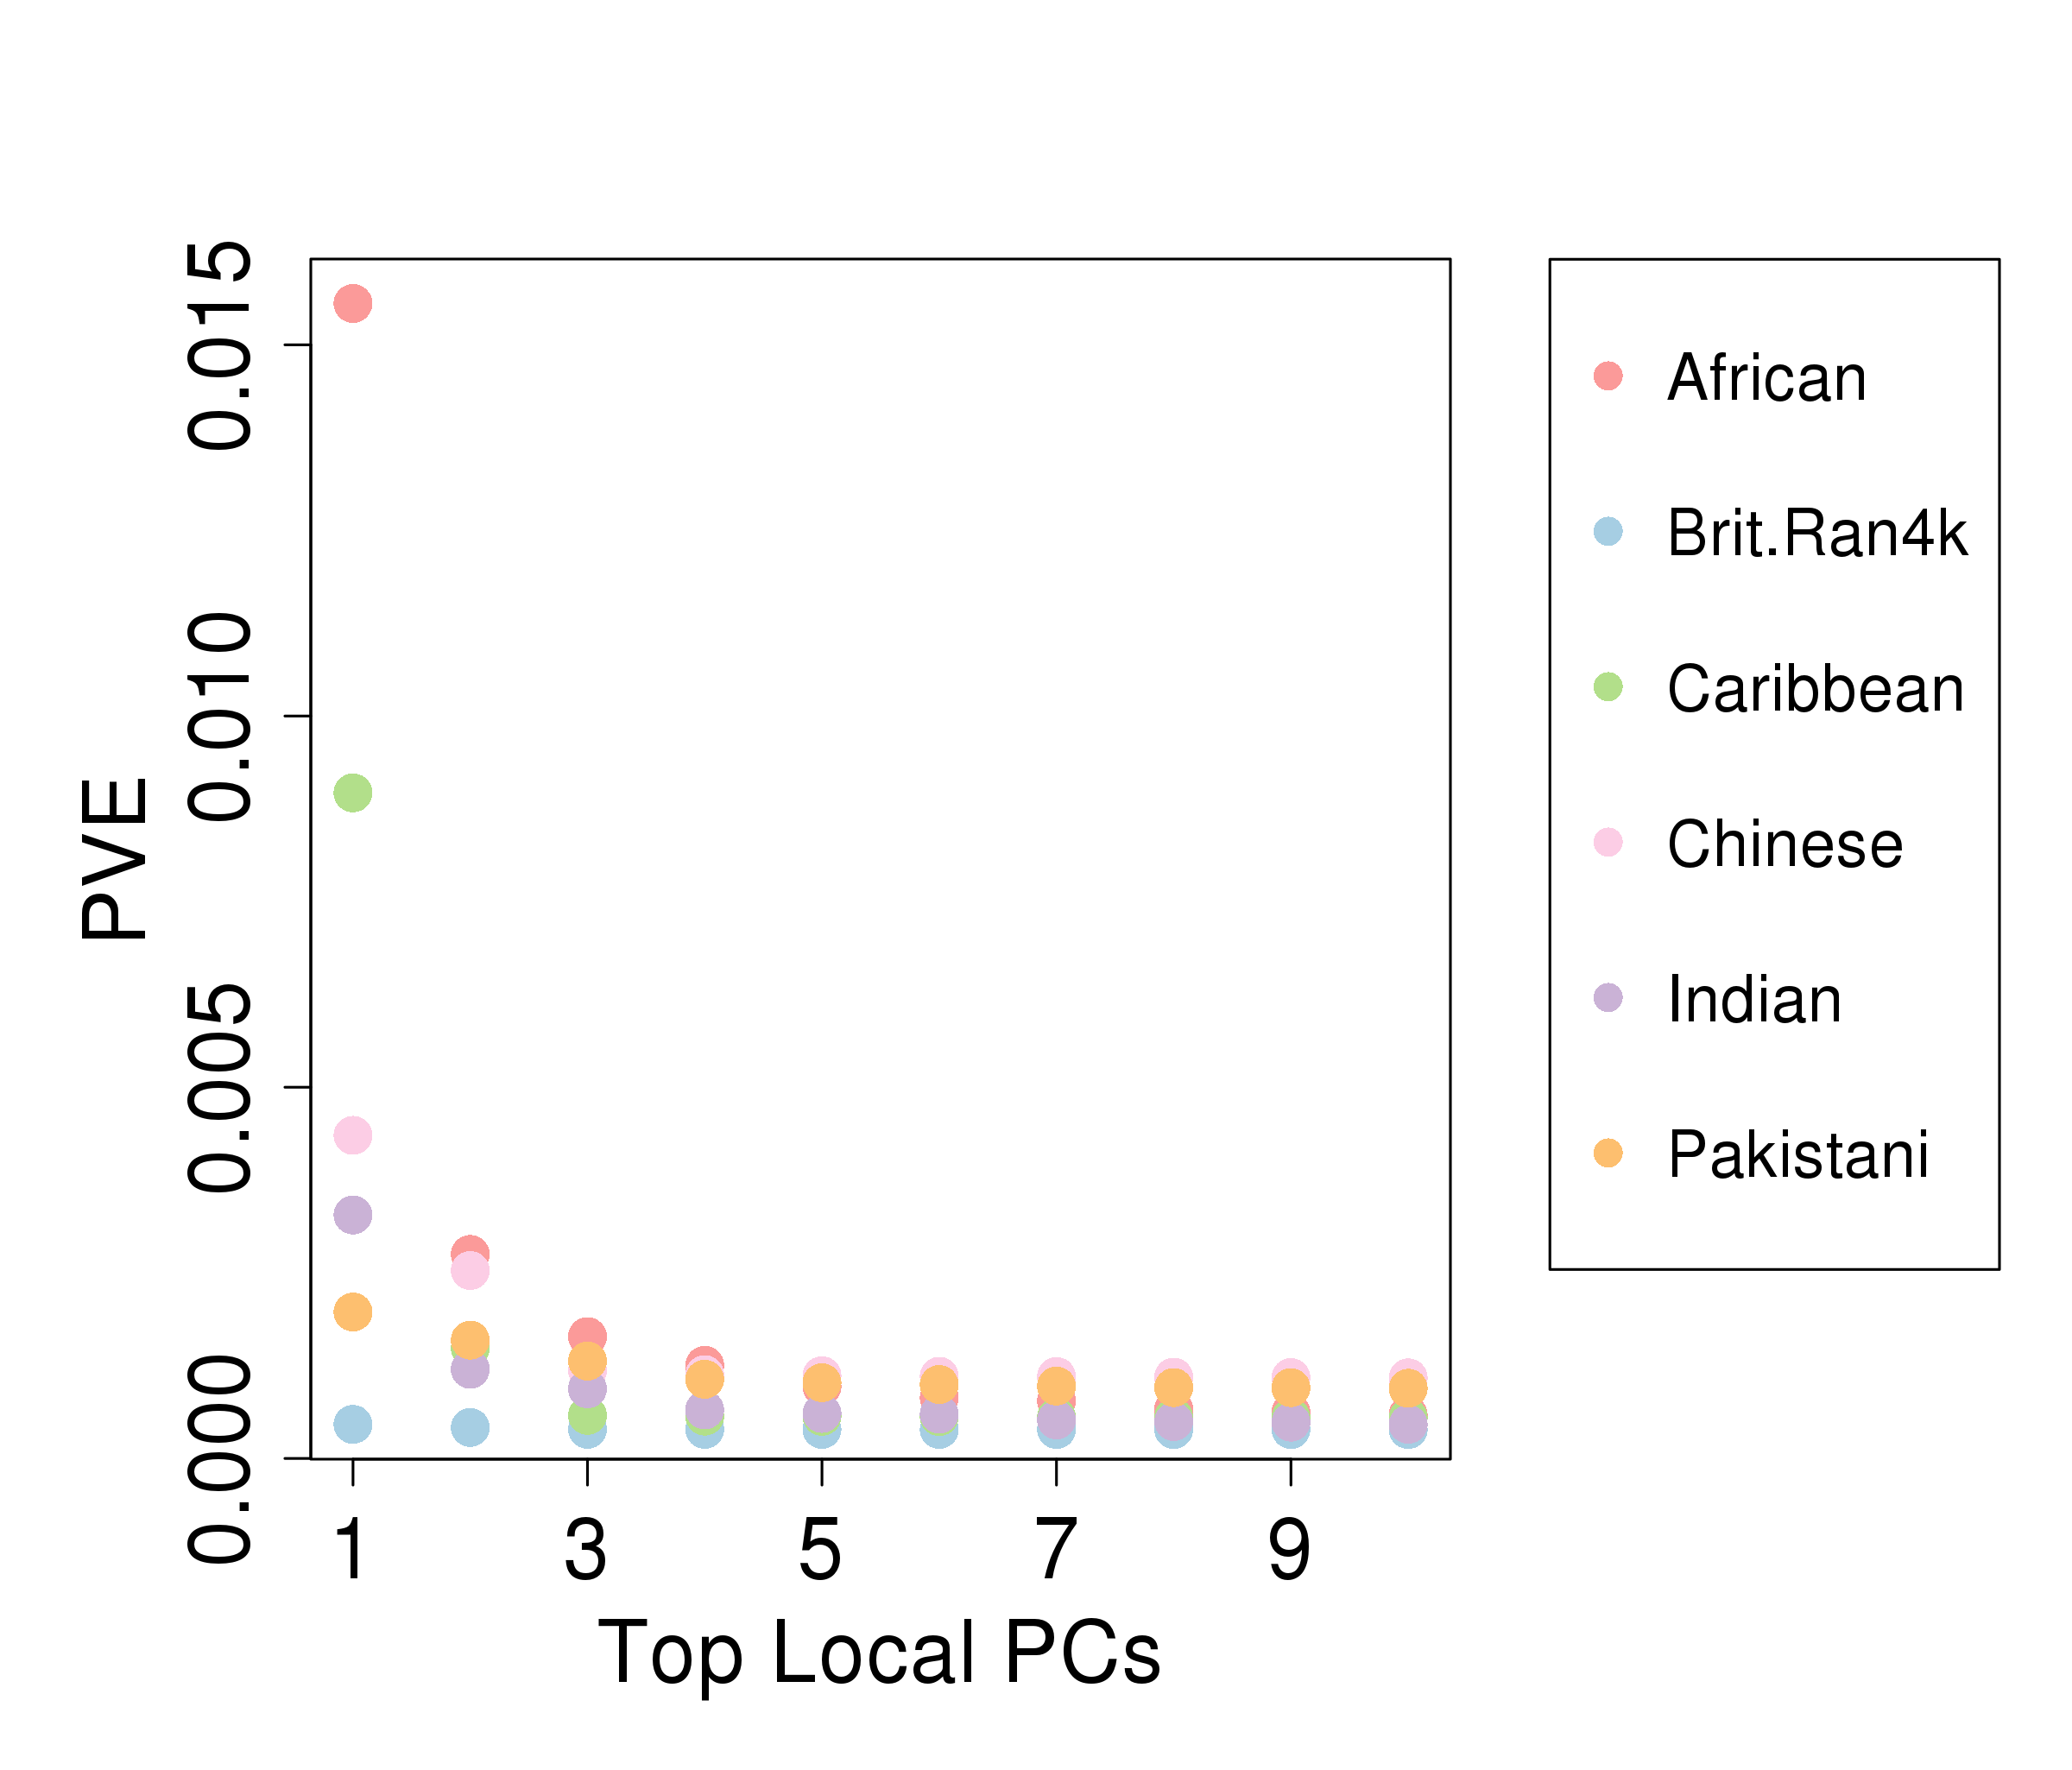
\includegraphics[scale=.45]{Images/Main/InterPath_Main_Figure_Eigenvalues_vs2.png}
\caption[TBD]{\textbf{Distribution of top 10 local principal component PVEs across UKB subgroups}. The plot shows the PVE of each of the top 10 local PCs for each of our UKB population subgroups. Local here continues to refer to calculating PCs within each subgroup separately (versus calculating PCs jointly across all subgroups together). We observe that the distribution of PC1 PVEs among the subgroups appears to match the distribution of total number of genome-wide significant MAPIT-R pathways we identify per subgroup (see Figure \ref{InterPath-Main-Figure-Barplots-KEGG} and  Supplementary Figure \ref{InterPath-Supp-Figure-Barplots-REACTOME}).}
\label{InterPath-Main-Figure-Eigenvalues}
\end{figure}

One other possibility is that PC space, while revealing a possible connection between how population structure heterogeneity among subgroups may affect MAPIT-R results, is not sensitive enough for a pathway-level analysis. Another representation of population structure that may be more ancestry-specific, and therefore more sensitive, is local ancestry estimates. Because the African subgroup contains admixture, we can test whether pathways that have a greater proportion of local African ancestry are more likely to have lower MAPIT-R $p$-values. To do this, we ran RFMix \citep{Maples2013} on the African subgroup with the 1000 Genomes CEU and YRI \citep{Genomes2015} populations as outgroups to calculate per individual estimates of local African ancestry, and we then derived subgroup-wide average local ancestry estimates across all individuals. To get final pathway-level metrics of local ancestry, we calculated the average overlap a pathway has with regions of the genome that have local African ancestry. We then tested each pathway's proportion of local African ancestry against its MAPIT-R $p$-value to see if this more ancestry-specific form of population structure has a relationship to the large number of MAPIT-R results the African subgroup has. However, as Figure \ref{InterPath-Main-Figure-RFMix-African-REACTOME} and Supplementary Figure \ref{InterPath-Supp-Figure-RFMix-African-KEGG} show, we find no relationship between a pathway's proportion of local African ancestry and its MAPIT-R $p$-value.

\begin{figure}[htb]
\centering
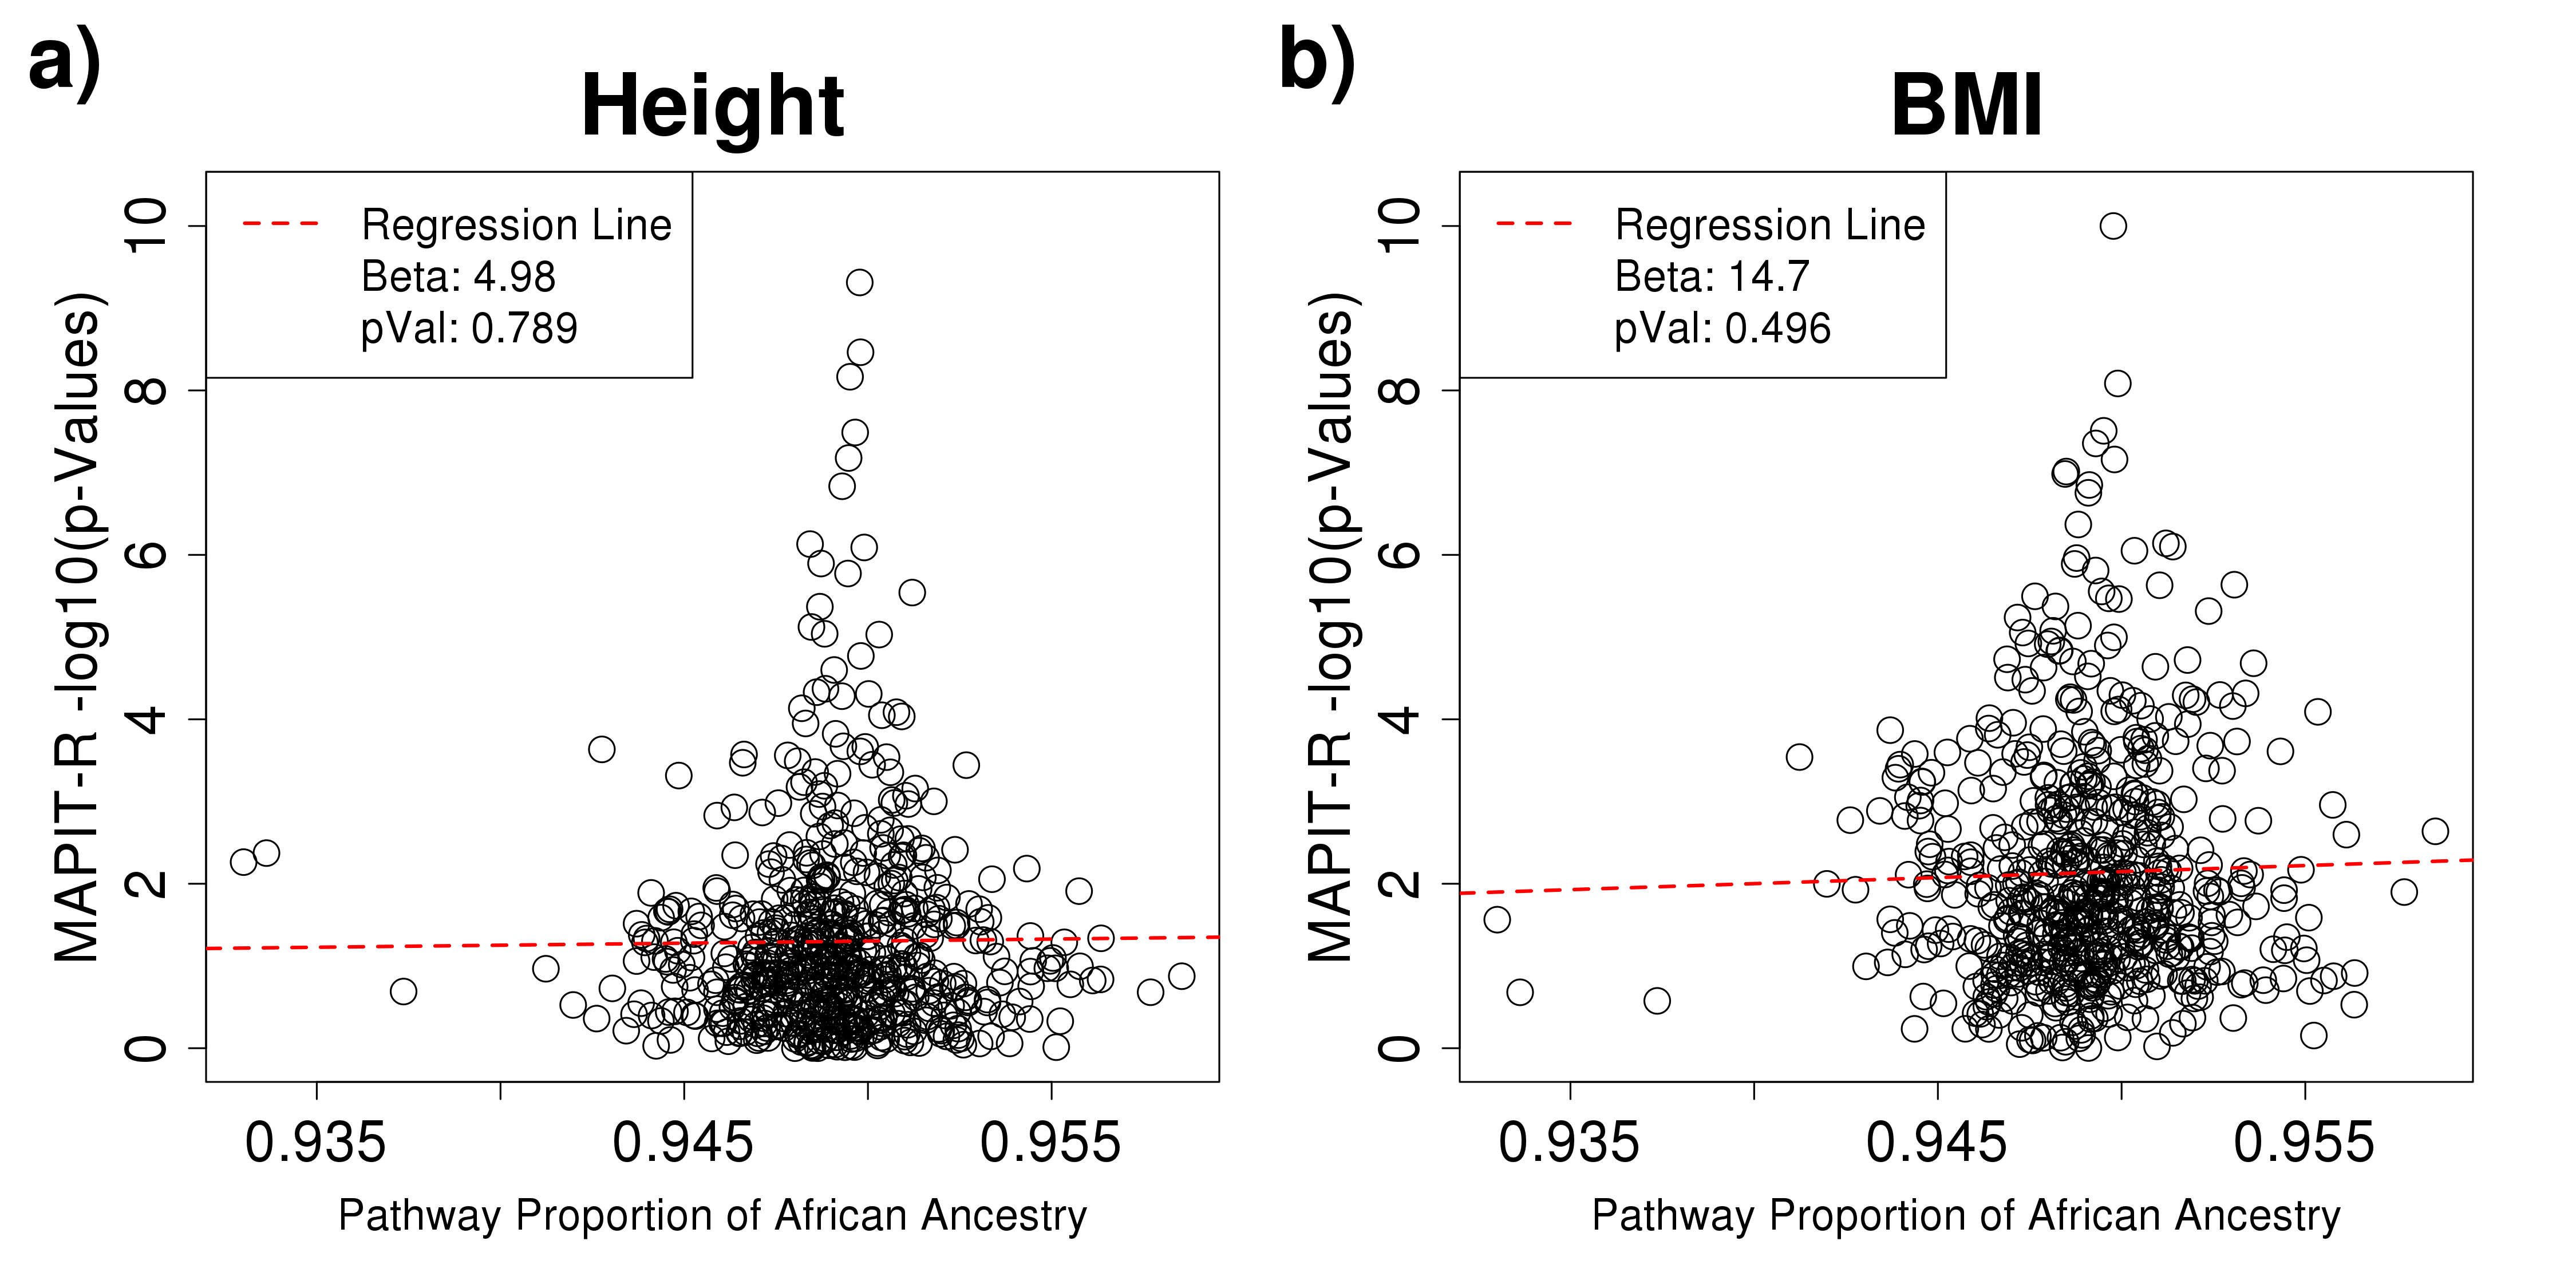
\includegraphics[scale=.35]{Images/Main/InterPath_Main_Figure_RFMix_vs2_African_REACTOME_noHLA.png}
\caption[TBD]{\textbf{MAPIT-R results vs. proportion of local African ancestry per REACTOME pathway}. The figure shows MAPIT-R $p$-values per pathway plotted against each pathway's proportion of local African ancestry for each REACTOME (a) height and (b) BMI analysis. Proportions of African ancestry are shown on the $x$-axis and MAPIT-R $p$-values are shown on the $y$-axis. African ancestry proportions were calculated per individual by using RFMix with the 1000 Genomes CEU and YRI populations as outgroups and then genome-wide averages were taken across the subgroup. Per pathway proportions of African ancestry were derived by taking the average of the subgroup-wide estimates of African ancestry across the regions of the genome that each pathway overlapped.}
\label{InterPath-Main-Figure-RFMix-African-REACTOME}
\end{figure}

\section{Discussion}\label{InterPath-Discussion}

Here we present the first scans for marginal epistasis within multiple human ancestries as well as at the pathway-level. We implement a new method, MAPIT-R, to test for epistasis between pathways and the rest of the genome and apply it in six different human ancestries sampled in the UK Biobank (African, British, Caribbean, Chinese, Indian, and Pakistani). Using two different  pathway databases and measurements of height and BMI, we find a total 245 pathways that have significant epistatic interactions with the rest of the genome. We find that the African subgroup produces the majority of these results, with over 65\% of our 245 significant pathways being identified within the African subgroup. We find that pathways related to immunity, cellular signaling, and metabolism have significant signals in our genome-wide marginal epistasis scans, and that BMI produces more significant marginal epistatic interactions at the pathway level than height. In testing for drivers of our MAPIT-R results, we find evidence that the proteasome may be enriched for marginal epistatic interactions and characterize how proteasome gene families contribute to pathway-level marginal epistatic signals. 

The fact that we find such an abundance of epistatic signals in the African subgroup underscores that African populations, and non-European ancestries in general, are particularly useful for complex trait genetics \citep{Dumitrescu2011,Rotimi2017,Choudhury2018,Martin2018,Mogil2018,Bien2019,Kuchenbaecker2019,Wojcik2019,Zhong2019,Bentley2020}. Past research has shown that African ancestry genomes offer a more complete characterization of the the genetic architecture of skin pigmentation \citep{Martin2017b,Crawford2017b}, reveal the evolutionary histories of FOXP2 and other loci \citep{Atkinson2018,Sugden2018}, and are needed for more transferable polygenic risk scores \citep{Duncan2019,Marnetto2020}. While many studies have generated a call for more GWA studies to be conducted in individuals of non-European ancestry  \citep{Need2009,Popejoy2016,Gurdasani2019,Martin2019,Sirugo2019}, we believe this study reveals that our understanding of the role of epistasis in human complex trait architecture will also expand with multiethnic analyses.  Our results suggest that non-European ancestries, and African ancestries in particular, may be better suited for identifying signals of epistasis than European ancestries. 

Our analyses are not without limitations. First, we are limited due to the computational costs of epistasis detection; although testing for  marginal epistasis reduces our testing burden from standard epistasis scans, MAPIT and MAPIT-R do not scale well to the full sample sizes of modern human genomic biobanks.
Specifically, MAPIT-R  encounters burdensome computational times when analyzing beyond 10,000 individuals. An important direction for future research is to detect epistatic interactions using GWA summary statistics; moving from direct genotypes to GWA study summary statistics has proven useful in both speeding up computational time as well as increasing power in multiple other GWA contexts \citep{Shi2016,Johnson2018,Ray2018,Turchin2019,Urbut2019,Cheng2020}. Another limitation of MAPIT-R is that, as part of the marginal epistasis framework, it identifies whether a pathway contains \textbf{any} epistatic interactions with the rest of the genome. As shown here this has the advantage of accumulating signal over multiple variants, but it produces an ambiguous situation in terms of what regions of the genome to analyze \textit{a posteriori}. One strategy explored by \citet{Crawford2017a} is to conduct an exhaustive pairwise epistasis search among all MAPIT significant SNPs against the rest of the SNPs in the genome; extending a similar approach to MAPIT-R, we could conduct an exhaustive pairwise search between all variants present in our significant pathways against all variants remaining in the genome. Perhaps surprisingly given our sample sizes, doing such an exhaustive epistasis scan using our MAPIT-R pathway results does reveal five significant pairwise SNP interactions (Supplementary Table \ref{InterPath-Supp-Table-PairwiseEpi-Results}). But the multiple testing Bonferroni $p$-value correction step to identify these interactions are still very conservative and burdensome. Exploring marginal epistasis results \textit{a posteriori} can be further improved upon by using additional methodological approaches in GWAS. For example, linking MAPIT-R with a framework that explicitly follows up marginal epistasis signals with locus-focused methods such as fine-mapping \citep{Kichaev2014,Chen2015,Benner2016} or co-localization \citep{Hormozdiari2016,Zhu2016,Wen2017,Giambartolomei2018,Wallace2020} could even further expand the power of the marginal epistasis approach.  

\section{Methods}\label{InterPath-Online-Methods}

\subsection{UK BioBank Data}

\subsubsection{Population subgroups}

To create the UKB population subgroups used in this study, we first extracted and grouped individuals by the self-identified ancestries of `African', `British', `Caribbean', `Chinese', `Indian', and `Pakistani'. British random subgroups of 4,000 and 10,000 individuals, both the original sets and the additional four rounds of replications, were constructed by randomly choosing initial sets of non-overlapping 4,000 and 10,000 individuals. Standard quality control (QC) procedures were then employed on each population subgroup (see Supplementary Note for details) on both the variant and individual levels, pre-PCA. Local PCA was then conducted to confirm ancestry groupings and remove outliers. Note that the genetic data used in these analyses were the directly genotyped variant sets  from the UKB after running imputation on the University of Michigan Imputation Server \citep{Das2016}; most of the analyses in this manuscript utilize genetic relatedness matrices (GRMs), and GRMs require zero genotype missingness. To minimize the loss of SNPs while meeting this threshold we chose to impute missing genotypes while still focusing on just the original set of genotyped variants. For metrics and PCA plots of the final, post-QC set of UKB individuals, see Supplementary Figure \ref{InterPath-Supp-Figure-UKB-subgroups-PCAPlot} and Supplementary Table \ref{InterPath-Supp-Table-UKBPopStats}. British 4,000 and 10,000 random subgroups had lower final sample sizes due to the aforementioned QC procedures. 

\subsubsection{Phenotypes}

For the analyses presented in this study we focused on the complex traits of height and BMI. Each phenotype was adjusted for age, gender, and assessment center. Following previous pipelines \citep{Wood2014,Locke2015}, each dataset was first divided into males and females. Age was then regressed out within each sex, and the resulting residuals were inverse normalized. These normalized values were then combined back together between sexes and, lastly, assessment center designations were regressed out. For analyses using permuted phenotypes, permutations were conducted within-subgroup and done by randomly reassigning phenotypes to individuals.

\subsection{MAPIT-R Model}

\textcolor{red}{Reminder: we regress the additive genotypes out of the phenotype now instead of including that information in the m-projection matrix}

We describe the framework for ``\underline{Inter}actions in \underline{Path}way'' (MAPIT-R) analysis in detail here. The key goal of this method is to identify crosstalk between signaling pathways in GWA studies, without having to explicitly model all possible higher-order interactions. In general, consider a pathway which is defined by a set of SNPs found within the regulatory regions of genes in that pathway. We will denote these variants with the set of indices $\mathcal{R} = (r_1,\ldots,r_p)$. Begin by considering the following partitioned linear regression model,
\begin{equation}\label{LM}
\by = \mu\bm{1}+\sum_{r\in \mathcal{R}}\bx_r\beta_{r}+\sum_{s\not\in \mathcal{R}}\bx_s\beta_{s}+\bvarepsilon, \quad \bvarepsilon\sim \mathcal{N}(\mathbf{0}, \tau^2\bI),
\end{equation}
where $\by$ is an $n$-dimensional vector of quantitative phenotypes for $n$ individuals; $\mu$ is an intercept term with an $n$-dimensional vector of ones; $\bx_r$ and $\bx_s$ are $n$-dimensional genotype vectors for variants that lie within and outside the regulatory region $\mathcal{R}$, respectively; $\beta_r$ and $\beta_s$ are the corresponding additive effect sizes; $\bvarepsilon$ is an $n$-vector of residual errors; $\tau^2$ is the residual error variance; $\bI$ denotes the identity matrix; and $\mathcal{N}(\bullet,\bullet)$ denotes a multivariate normal distribution. Here, we also assume that the genotypic vectors have been centered and standardized to have mean 0 and standard deviation 1.

Because we consider scenarios where there are more variants than samples, we need to specify additional modeling assumptions in Equation \eq{LM} to make the rest of the model identifiable. In particular, we recall previous approaches and assume that the individual effect sizes follow univariate normal distributions, or $\beta_r \sim \mathcal{N}(0, \omega^2/p)$ and $\beta_s \sim \mathcal{N}(0, \sigma^2/(l-p))$, where $l$ is the number of total number of all SNPs \citep{Crawford2017a}. With the assumption of normally distributed effect sizes, the model defined in Equation \eq{LM} is equivalent to a variance component model where $\bg\sim \mathcal{N}(\bm{0}, \omega^2\bK)$ with $\bK=\bX_{\mathcal{R}}\bX_{\mathcal{R}}^{\T}/p$ being the genetic relatedness matrix computed using genotypes from all variants within the signaling pathway of interest; and $\wt\bg\sim \mathcal{N}(\bm{0}, \nu^2\wt\bK)$ with $\wt\bK=\bX_{-\mathcal{R}}\bX_{-\mathcal{R}}^{\T}/(l-p)$ representing a relatedness matrix computed using all other variants. Note that $\bg$ may be interpreted as a pathway's additive effect, while $\wt\bg$ denotes its polygenic background. 

To complete the specification of the MAPIT-R methodology, we lastly assume an additional random effect $\bu$ which models the summation of all pairwise interaction effects between a given signaling pathway variant and all other pathways. In this work, we limit ourselves to the case of finding second order crosstalk relationships between pathways --- although, extensions to higher-order interactions is straightforward \citep{Crawford2017a}. Altogether, this results in the following linear mixed model
\begin{equation}
\by = \mu\bm{1}+ \bg +\wt\bg+\bu+\bvarepsilon,\\ 
\bg\sim \mathcal{N}(\bm{0}, \omega^2\bK), \quad \wt\bg\sim \mathcal{N}(\bm{0},
\nu^2\wt\bK),\\ 
\bu\sim\mathcal{N}(\bm{0},\sigma^2\bQ), \quad \bvarepsilon\sim \mathcal{N}(\mathbf{0}, \tau^2\bI).\label{LMM}
\end{equation}
Here, the $\bQ = \bK\circ\wt\bK$ is represents a second-order interaction relationship matrix, and is obtained by using the Hadamard product (i.e.~the squaring of each element) between the pathway specific relatedness matrix and its corresponding polygenic background. Note that the formulation of MAPIT-R in Equation \eq{LMM} can easily be extended to accommodate other fixed effects (e.g.~age, sex, or genotype principal components), as well as other random effects terms that can be used to account for sample non-independence due to other genetic or common environmental factors.

%Note that we make the assumption that each $\bg_k^{(l)}\sim \mbox{MVN}(\bm{0}, \sigma_{l}^2\bK^l_k)$, where the baseline covariance matrix $\bK_k=\bX_{-\mathcal{R}}\bX_{-\mathcal{R}}^{\T}/p_k$ is the conventional genetic relatedness matrix computed using genotypes from all $p_k$ variants outside of the region $\mathcal{R}$. Here, we use the power factor $l$ to denote the order of interaction (epistatic) effects that are accounted for within the model. For example, when $l=2$, $\mathbf{K}_k^2 = \mathbf{K}_k\circ\mathbf{K}_k$ represents a pairwise interaction relationship matrix, and is obtained by using the Hadamard product (i.e.~the squaring of each element) of the linear kernel matrix with itself \citep{Henderson:1985aa,Ronnegard:2008aa,Jiang:2015aa}. In this case, $\mathbf{K}_k^2$ denotes the marginal second order epistatic effect of the $k$\textsuperscript{th} functional marker under the polygenic background of all other markers. It is important to note that each $\bK_k^{l}$ changes with every new gene, protein, or pathway $k$ that is considered.

\subsection{Hypothesis Testing for Interaction Effects}

Our goal is to identify signaling pathways that have significant non-zero interaction effects on a given phenotype. To do so, we examine each $r$-th pathway of interest in turn, and test the null hypothesis in Equation \eqref{LMM} that $\text{H}_0: \sigma^2=0$. The variance component $\sigma^2$ effectively captures the total interaction effects between the $r$-th pathway and all other pathways. We refer to this as the marginal interaction effect for the $r$-th pathway. To do so, we make use of the MQS method for parameter estimation and hypothesis testing \citep{Zhou2017}. Briefly, MQS is based on the computationally efficient method of moments and produces estimates that are mathematically identical to the Haseman-Elston (HE) cross-product regression \citep{Haseman1972}. To estimate the variance components with MQS, we first multiply Equation \eq{LMM} by a projection (hat) matrix onto the null space of the intercept term $\mu$, where $\bH=\bI-\bm{1}(\bm{1}^{\T}\bm{1})^{-1}\bm{1}^{\T}$. After this projection procedure, we obtain a simplified linear mixed model 
\begin{equation}
\by^*_r = \bg^*_r +\wt\bg^*_r+\bu^*_r+\bvarepsilon^*_r\\ 
\bg_r\sim \mathcal{N}(\bm{0}, \omega^2\bK^*_r), \quad \wt\bg_r\sim \mathcal{N}(\bm{0}, \nu^2\wt\bK^*_r),\\ \bu_r\sim\mathcal{N}(\bm{0},\sigma^2\bQ^*_r), \quad \bvarepsilon_r\sim \mathcal{N}(\mathbf{0}, \tau^2\bH) \label{LMM2}
\end{equation}
where $\by^*_r=\bH\by$; $\bg^*_r = \bH\bg_r$; $\bK^*_r = \bH\bK_r\bH$; $\wt\bg_r^* = \bH\wt\bg_r$; $\wt\bK_r^* = \bH\wt\bK_r\bH$; $\bu^*_r = \bH\bu_r$; $\bQ^*_r = \bH\bQ_r\bH$; and $\bvarepsilon_r^* = \bH_r\bvarepsilon$, respectively. Then for each pathway considered, the MQS estimate for the marginal interaction effect is computed as
\begin{equation}
\wh\sigma^2 = \by^{*\T}_r\bA_r\by
\end{equation}
where $\bA_{r} = (\bS_r^{-1})_{31}\bK_r^*+(\bS_r^{-1})_{32}\wt\bK_r^*+(\bS_r^{-1})_{33}\bQ^*_r+(\bS_r^{-1})_{34}\bH$ with elements $(\bS_r)_{jk} = \tr(\bSigma_{rj} \bSigma_{rk})$ for the covariances matrices subscripted as $[\bSigma_{r1}; \bSigma_{r2}; \bSigma_{r3}; \bSigma_{r4}]  = [\bK^*_r; \wt\bK^*_r; \bQ^*_r; \bH]$. Here, $\tr(\bullet)$ is used to denote the matrix trace function. It has been shown that, under MQS, a given marginal variance component estimate $\wh\sigma^2$ follows a mixture of chi-square distributions under the null hypothesis \citep{Crawford2017a}. Namely, $\wh\sigma^2 \sim \sum_{i=1}^{n}\lambda_{i}\chi^2_{1,i}$, where $\chi^2_{1}$ are chi-square random variables with one degree of freedom and $(\lambda_{1},\ldots,\lambda_{n})$ are the eigenvalues of the matrix 
\begin{equation*}
\left(\wh\omega^2_{0}\bK^*_r+\wh\nu^2_{0}\wt\bK^*_r+\wh\tau^2_{0}\bH\right)^{1/2} \bA_{r}\left(\wh\omega^2_{0}\bK^*_r+\wh\nu^2_{0}\wt\bK^*_r+\wh\tau^2_{0}\bH\right)^{1/2}
\end{equation*}
with $(\wh\omega^2_{0},\wh\nu^2_{0},\wh\tau^2_{0})$ being the MQS estimates of $(\omega^2,\nu^2,\tau^2)$ under the null hypothesis. Several approximation and exact methods have been suggested to obtain p-values under the distribution of $\wh\sigma^2$. One frequented choice is Davies exact method \citep{Davies1980,Wu2011}. 

%\subsection*{Hypothesis Testing for Overall Associations}

%FORCE also provides an option for summarizing overall marker enrichment. Here, we assume that we have already computed the $q$ marginal effect p-values for genetic marker $k$, denoted as $\wh\bp_k = (\wh p_{k1},\ldots,\wh p_{kq})$. Let $\wh\balpha_k^* = F^{-1}(\wh\bp_k)$ be the transformed test statistic where $F^{-1}$ is the inverse of the cumulative distribution function (CDF) of the standard chi-square $\chi^2_1$. We follow previous works and define the sum of the correlated chi-square variables for a given functional genomic marker as \citep{Nakka:2016aa}
%\begin{equation}
%\bar{\alpha}_k^* = \sum_{l=1}^{q}\wh\alpha_{k,l}^*.\label{Comp}
%\end{equation}
%(NOTE: Follow the rest of the language from methods in PEGASUS here).


%Add note about MAPIT-R being in an R package at the end of Lorin's material?
\subsection{MAPIT-R Analyses}

MAPIT-R analyses were conducted by using code built on the modeling and testing described above. SNPs were mapped to pathways by first being mapped to genes, which were then aggregated together determined by the gene-based definitions of pathways the KEGG and REACTOME databases provide. KEGG and REACTOME pathway definitions were downloaded and extracted from the Broad Institute's MSigDB `C2: Curated Gene Sets' collection of pathways (\url{https://www.gsea-msigdb.org/gsea/msigdb/collections.jsp#C2}; \citep{Liberzon2011}). SNPs were annotated using Annovar \citep{Wang2010a} and were then mapped to a given gene if they were exonic, intronic, in the 5' and 3' UTRs, and 20kb upstream or downstream of the gene. Phenotypes were adjusted for age, sex, and assessment center (see `Phenotypes'). The top 10 `local' principal components (PCs) were included as covariates during the MAPIT-R analyses; `local' here refers to conducting PCA within each subgroup individually versus a `global' set up of conducting PCA on every subgroup together jointly. Note that due to numerical precision limitations within the R package `CompQuadForm', which is used to calculate final $p$-values, $p$-values < 1E-10 default to 0; therefore for any analysis presented here where required, $p$-values that were returned as 0 were reassigned as 1E-10 or presented as `< 1E-10'. MAPIT-R R code and a tutorial are available on Github (\url{https://github.com/mturchin20/MAPITR}) or CRAN (\url{}).

\subsection{Hypergeometric enrichment analyses}

Hypergeometric analyses were conducted by counting the number of times a given gene is present among the MAPIT-R significant pathways for a given database-phenotype-subgroup combination versus the number of times the gene is present among the background distribution of pathways from the given database. For the size-restriction analyses, pathways with greater than 1,000 SNPs were removed from both the MAPIT-R significant pathways and the pathway database. 1,000 SNPs was chosen as the threshold as a balance between total number of pathways removed and distance from the max SNP pathway sizes across all subgroups jointly (see Supplementary Figure \ref{InterPath-Supp-Figure-pValsVsNumSNPs} for relationship between MAPIT-R $p$-value and SNP pathway sizes for all database-phenotype-subgroup combinations). However, for a number of size thresholds ranging from 500 to 1,500 SNPs, the proteasome gene families still stand out as being either the most improved in terms of more significant enrichment $p$-values after the size restriction step or one of the most improved collection of genes (Supplementary Figure \ref{InterPath-Supp-Figure-Hypergeoemtric-SizeThresholds}).

\subsection{MAPIT-R results versus genetic variation analyses}
\subsubsection{Pathway-level IBS analyses}

Pathway-level IBS analyses were conducted by first calculating per-pathway IBS metrics. These were derived by using PLINK's \texttt{--distance ibs} function \citep{Purcell2007} using only the SNPs present in each pathway and only the individuals within each subgroup one at a time. For a single subgroup-wide metric per-pathway, the average pathway IBS value was taken across all pairwise comparisons within a given subgroup. Comparisons were then made by comparing this single subgroup-wide, per-pathway IBS metric against each pathway's original MAPIT-R $p$-value.

\subsubsection{RFMix analyses}

RFMix analyses were conducted within the African subgroup by running local ancestry estimation with RFMix v2.03 \citep{Maples2013} and the 1000 Genomes CEU and YRI populations \citep{Genomes2015} as outgroups. Pathway-level metrics of local ancestry were then calculated by first taking the average local African estimates across all individuals within the subgroup for a given genomic region and then averaging these subgroup-wide values across all portions of the genome a pathway overlaps. This produced a single per-pathway metric of local African ancestry that was then used to compare against MAPIT-R $p$-values. Running two iterations of the RFMix EM step to refine local ancestry estimates did not change the results.

\subsubsection{PC1 SNP loading analyses}

PC1 SNP loading analyses were conducted by first calculating per-pathway metrics of PC1 SNP loading proportions. This was done by: a) deriving PC1 loading scores per SNP by projecting all SNPs back onto the `local' PC space previously calculated within each subgroup, b) determining the distribution of local PC1 loading scores across all SNPs and designating SNPs within the 2.5\% tails of these distributions as `strongly loaded' on PC1, and c) calculating the proportion of SNPs per pathway that are designated as local PC1 `strongly loaded'. Given these per-pathway proportions of `strongly loaded' local PC1 SNPs then, comparisons where made between them and each pathway's MAPIT-R $p$-value. Using percent thresholds of 5\% or 10\% in the tails of the local PC1 loading score distributions to determine `strongly loaded' SNPs did not change the results (data not shown).

\section{URLs}\label{InterPath-URLs}

MAPIT: \url{https://github.com/lorinanthony/MAPIT}

MAPIT-R: \url{https://github.com/mturchin20/MAPIT-R}

\section{Acknowledgments}\label{InterPath-Acknowledgments}

This material is based upon work supported by the National Science Foundation under Grant No. DMS-1439786 while G.D. was in residence at the Institute for Computational and Experimental Research in Mathematics in Providence, RI, during the model and dimension reduction in uncertain and dynamic systems program.

\section{Author Contributions}\label{InterPath-Author-Contributions}

\section{Competing Interests}\label{InterPath-Competing-Interests}

\section{Supplementary Note}\label{Supplementary-Note}

\subsection{Population Subgroup Quality Control}

We conducted standard quality control (QC) procedures on each of these population subgroups. Note that we focused our analyzes on the genotyped chip data throughout the project. First we conducted SNP-level QC by dropping variants that did not meet the following criteria:  minor allele frequency (MAF) $>$ .01, genotype missingness $<$ 5\%, and Hardy-Weinberg equilibrium test $p$-value $>$ $1\times10^{-6}$. We then conducted individual-level QC via the following steps. Individuals were removed if they did not have genotype missingness $>$ 5\%. Individuals were also removed if they were a 3\textsuperscript{rd} degree relative or more to someone else in the dataset; specifically the KING relatedness values provided with the UKB data were used to identify related individuals, and one individual from every pair of 3\textsuperscript{rd} degree or more relatives was removed. Individuals were also dropped if they were tagged by any of the following three flags from the UKB data: `het.missing.outliers', `putative.sex.chromosome.aneuploidy', and `excess.relatives'. Lastly, individuals were removed if they were determined to be PCA outliers; this was conducted by running FlashPCA (version 2.1) \citep{Abraham2017} in R on each population subgroup separately and identifying individuals that had PC values greater than 7 standard deviations away from the mean for any of the top 6 PCs. We refer to conducting PCA on each subgroup separately as 'local PCA' to help distinguish from the alternative setup of conducting PCA on the entire dataset jointly, which would be referred to as 'global PCA'. 

After this first round of QC procedures, we then proceeded to impute our current population subgroups. Since most of the analyses in this project utilized genetic relatedness matrices (GRMs), and variants need to have no missing data for these GRMs, we used imputation primarily to maximize the number of genotyped SNPs that would not be dropped by this stringent threshold (as opposed to using imputation to increase the number of SNPs we were analyzing). To conduct this imputation, we uploaded our population subgroups to the University of Michigan Imputation Server \citep{Das2016} and used the following options: Minimac3 for the imputation software, 1000G phase 3 v5 for the reference panel, and Eagle v2.3 for the phasing software. Completed imputed files were then downloaded from the Imputation Server afterwards and treated to further QC steps: imputed variants were intersected back to the original set of genotyped chip variants, variants with imputation quality scores $<$ .3 were removed, and variants that had genotype missingness rates $>$ 0\% were also removed. These steps represent the last of our QC and imputation procedures, and information on the final forms of our UKB population subgroups can be found in Supplementary Table (table).

\clearpage

\section{Supplementary Figures}\label{Supplementary-Figures}

%\renewcommand{\thefigure}{Supplementary Figure \arabic{figure}}
%\renewcommand{\thetable}{Supplementary \arabic{table}}
\renewcommand{\figurename}{Supplementary Figure}
\renewcommand{\tablename}{Supplementary Table}
\setcounter{figure}{0}
\setcounter{table}{0}

\begin{figure}[htbp]
\centering
\hspace*{-1cm}
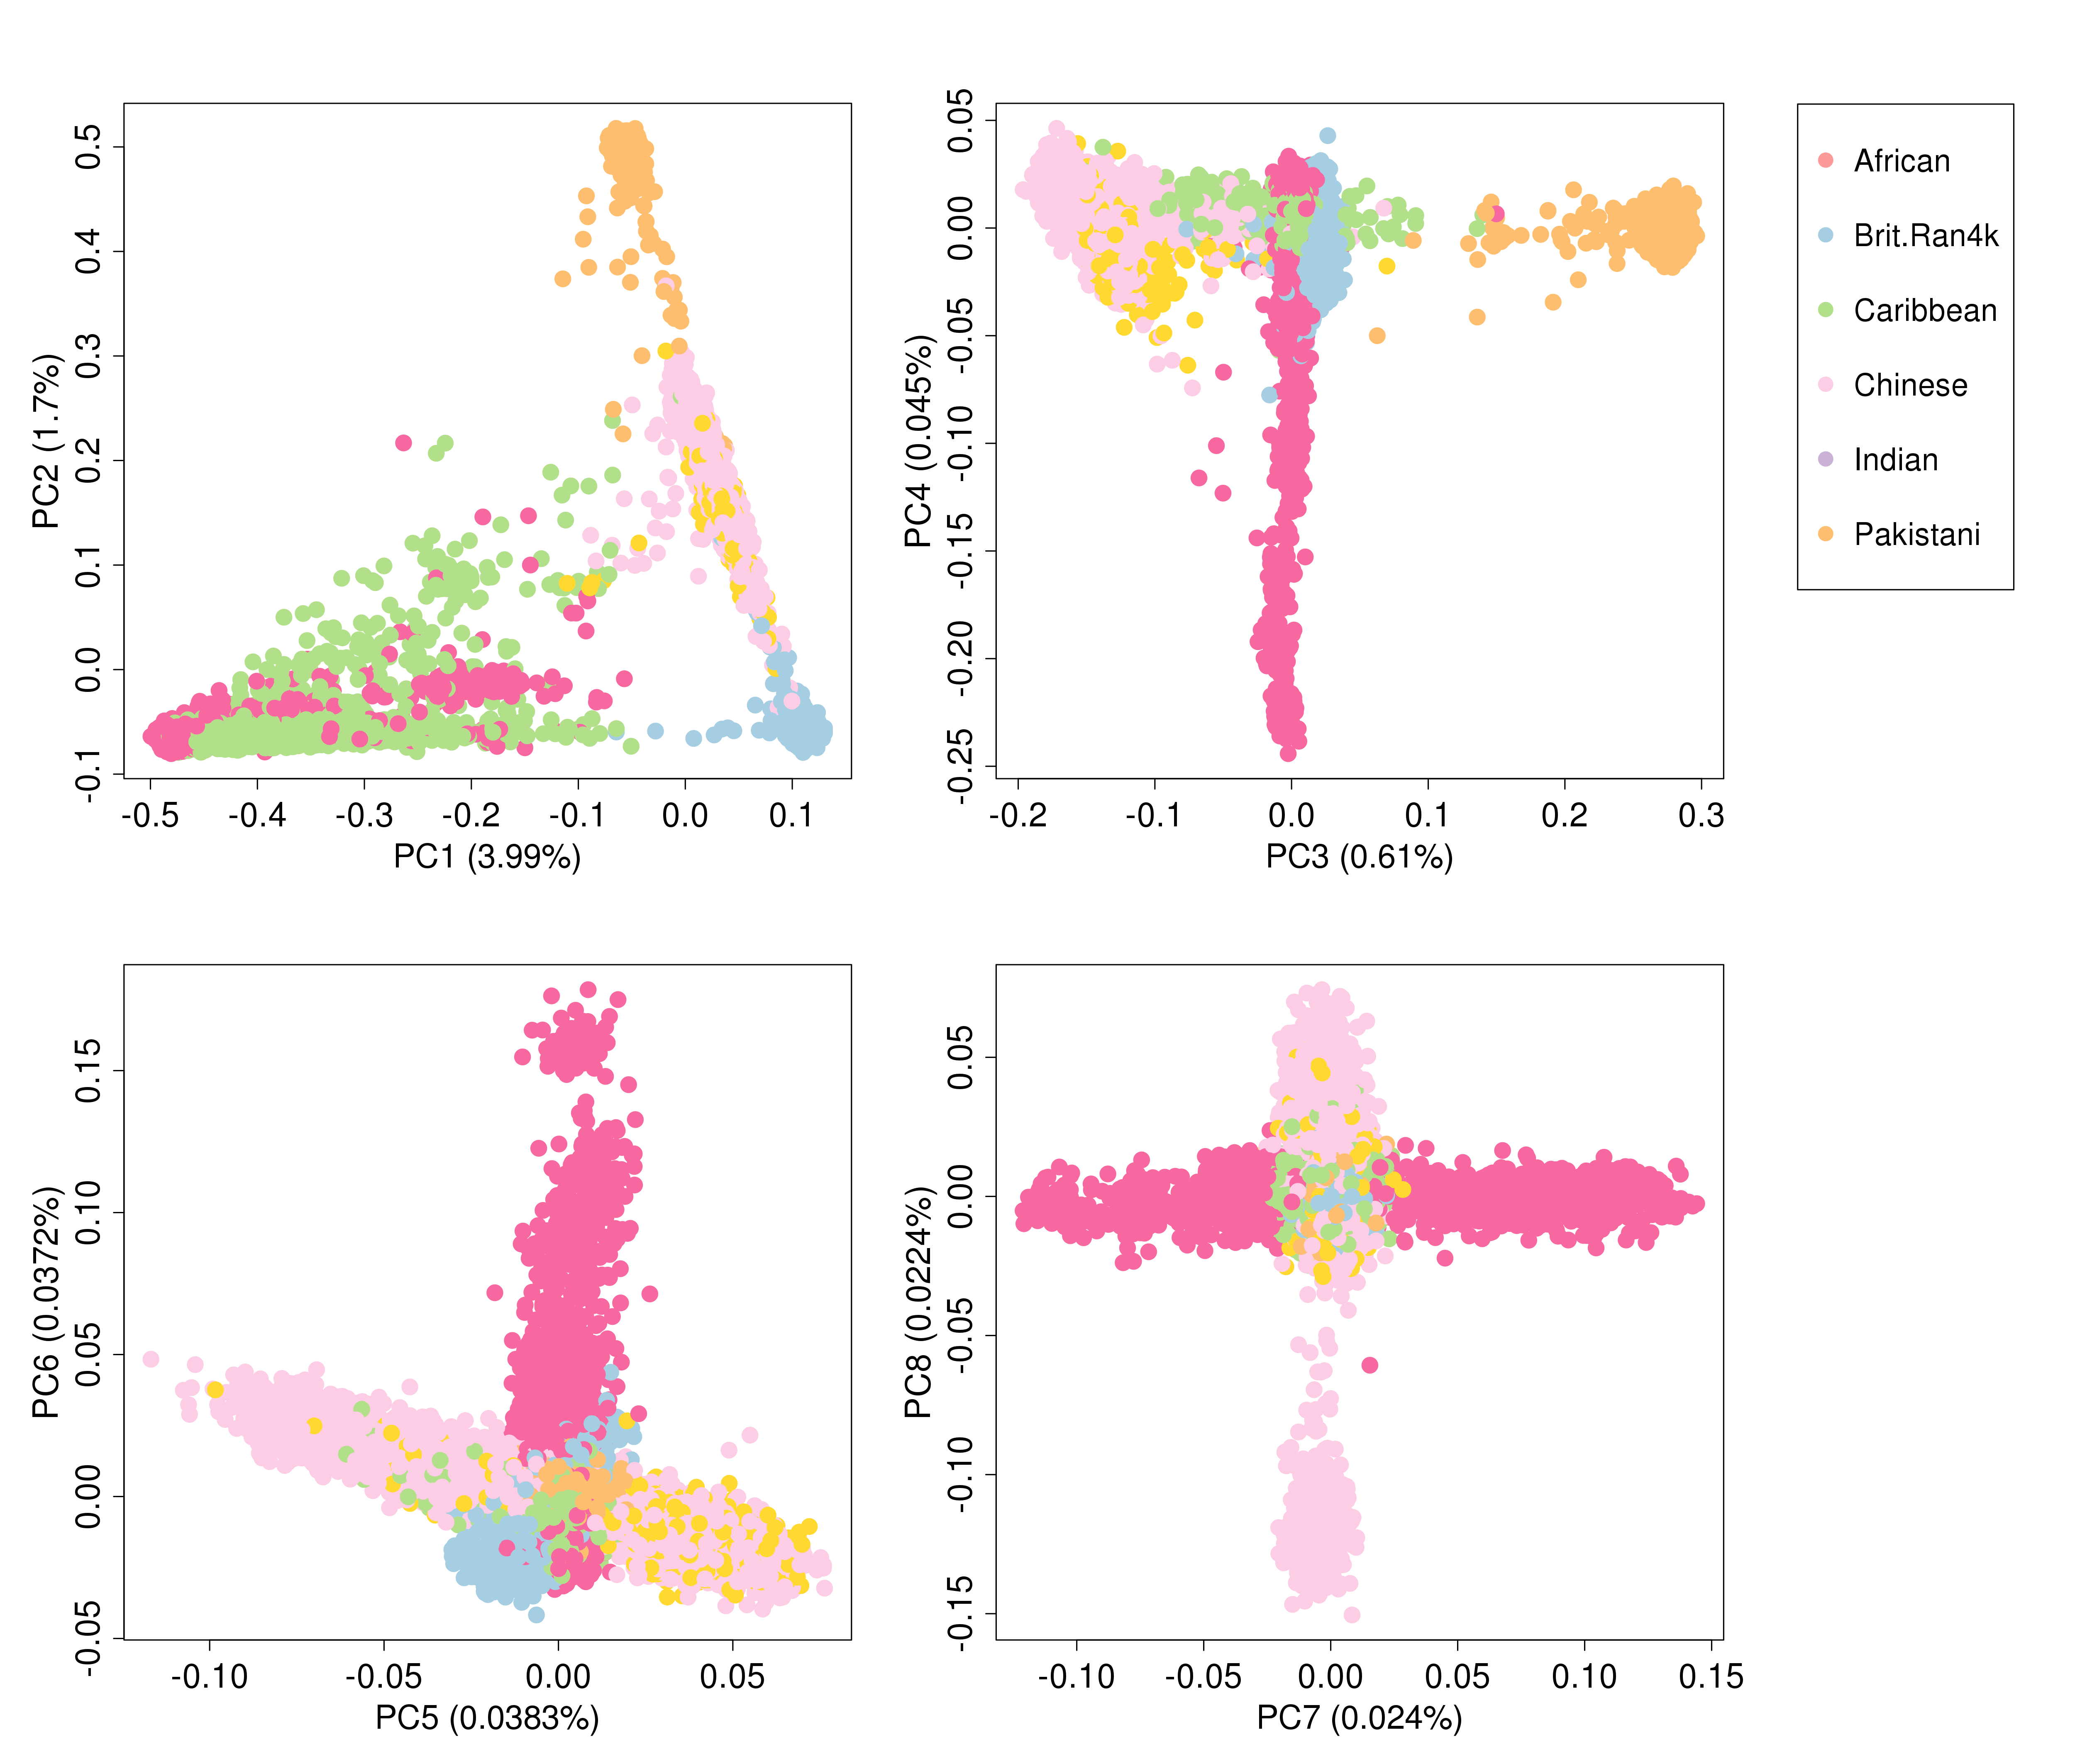
\includegraphics[scale=.4]{Images/Supp/InterPath_Supp_Figure_UKB_PCAPlot_vs2.png}
\caption[TBD]{\textbf{Global PCA Plots of the UK BioBank subgroups}. The figure shows the top eight global principal components (PCs) of our UKB subgroup dataset plotted against one another: (a) PC1 vs. PC2, (b) PC3 vs. PC4, (c) PC5 vs. PC6, and (d) PC7 vs. PC8. PCA was conducted using FlashPCA \citep{Abraham2017} and a post-QC, pruned SNP set. Here `Global' PCs refers to PCs calculated from running PCA on the full dataset of all subgroups together jointly. This is in contrast to `local' PCs, which are calculated by running PCA on each subgroup separately. As a result of this difference, global PCs were created similar to the descriptions in `Population subgroups' of Methods and `Population Subgroup Quality Control' of Supplementary Note, but in lieu of running FlashPCA on each subgroup separately, FlashPCA was run on the full dataset together jointly. Global PCs were only used for these plots, and local PCs were used for quality control and as covariates. In parentheses next to each PC is the percent variance explained (PVE) each PC accounts for of the total variation present in the underlying covariance matrix.}
\label{InterPath-Supp-Figure-UKB-subgroups-PCAPlot}
\end{figure}
\clearpage

\begin{figure}[htbp]
\centering
\hspace*{-.9cm}
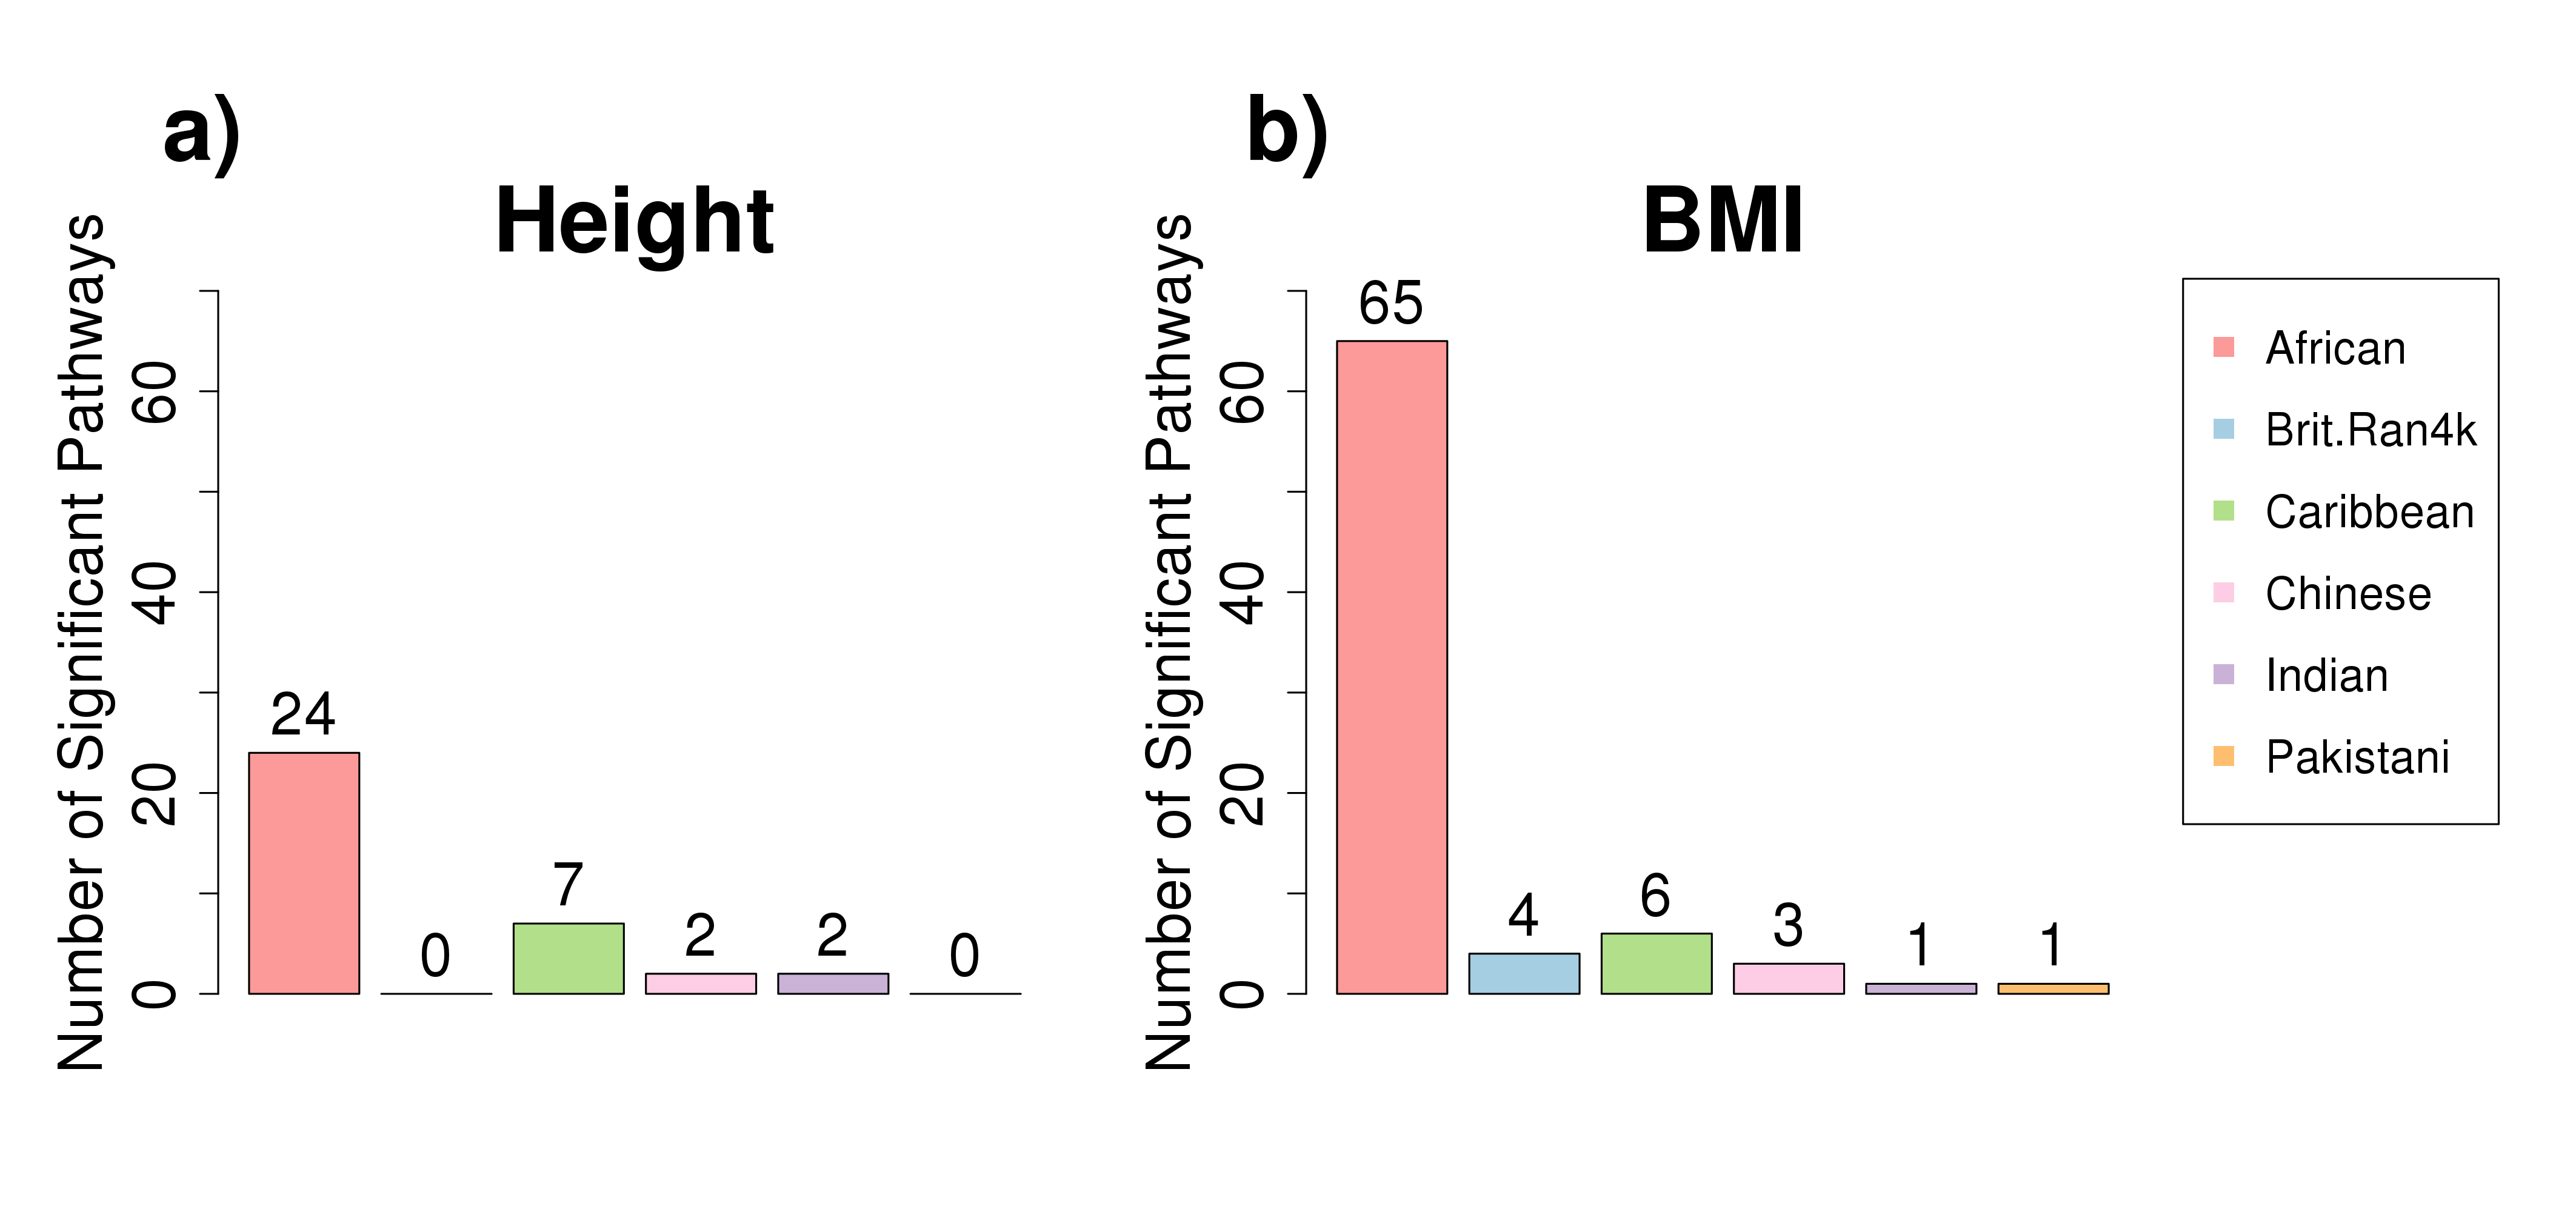
\includegraphics[scale=.45]{Images/Supp/InterPath_Supp_Figure_Barplots_REACTOME_vs4.png}
\caption[TBD]{\textbf{Numbers of REACTOME pathways that have significant marginal epistasis, per subgroup}. The barplots show the number of genome-wide significant pathways found from running MAPIT-R for both (a) height and (b) BMI in the REACTOME database on each of our UKB subgroups. Genome-wide significance was determined by using Bonferroni-corrected $p$-value thresholds based on the number of pathways tested in each pathway database-phenotype-subgroup combination. As shown in these results, we find across all database-phenotype combinations that the African subgroup has the largest numbers of significant pathways. For lists of the specific significant pathways per database-phenotype-subgroup combination, see Supplementary Tables \ref{InterPath-Supp-Table-TopPathways-AllPaths-AllPhenos}\textcolor{blue}{a-d}.}
\label{InterPath-Supp-Figure-Barplots-REACTOME}
\end{figure}
\clearpage

\begin{figure}[htbp]
\centering
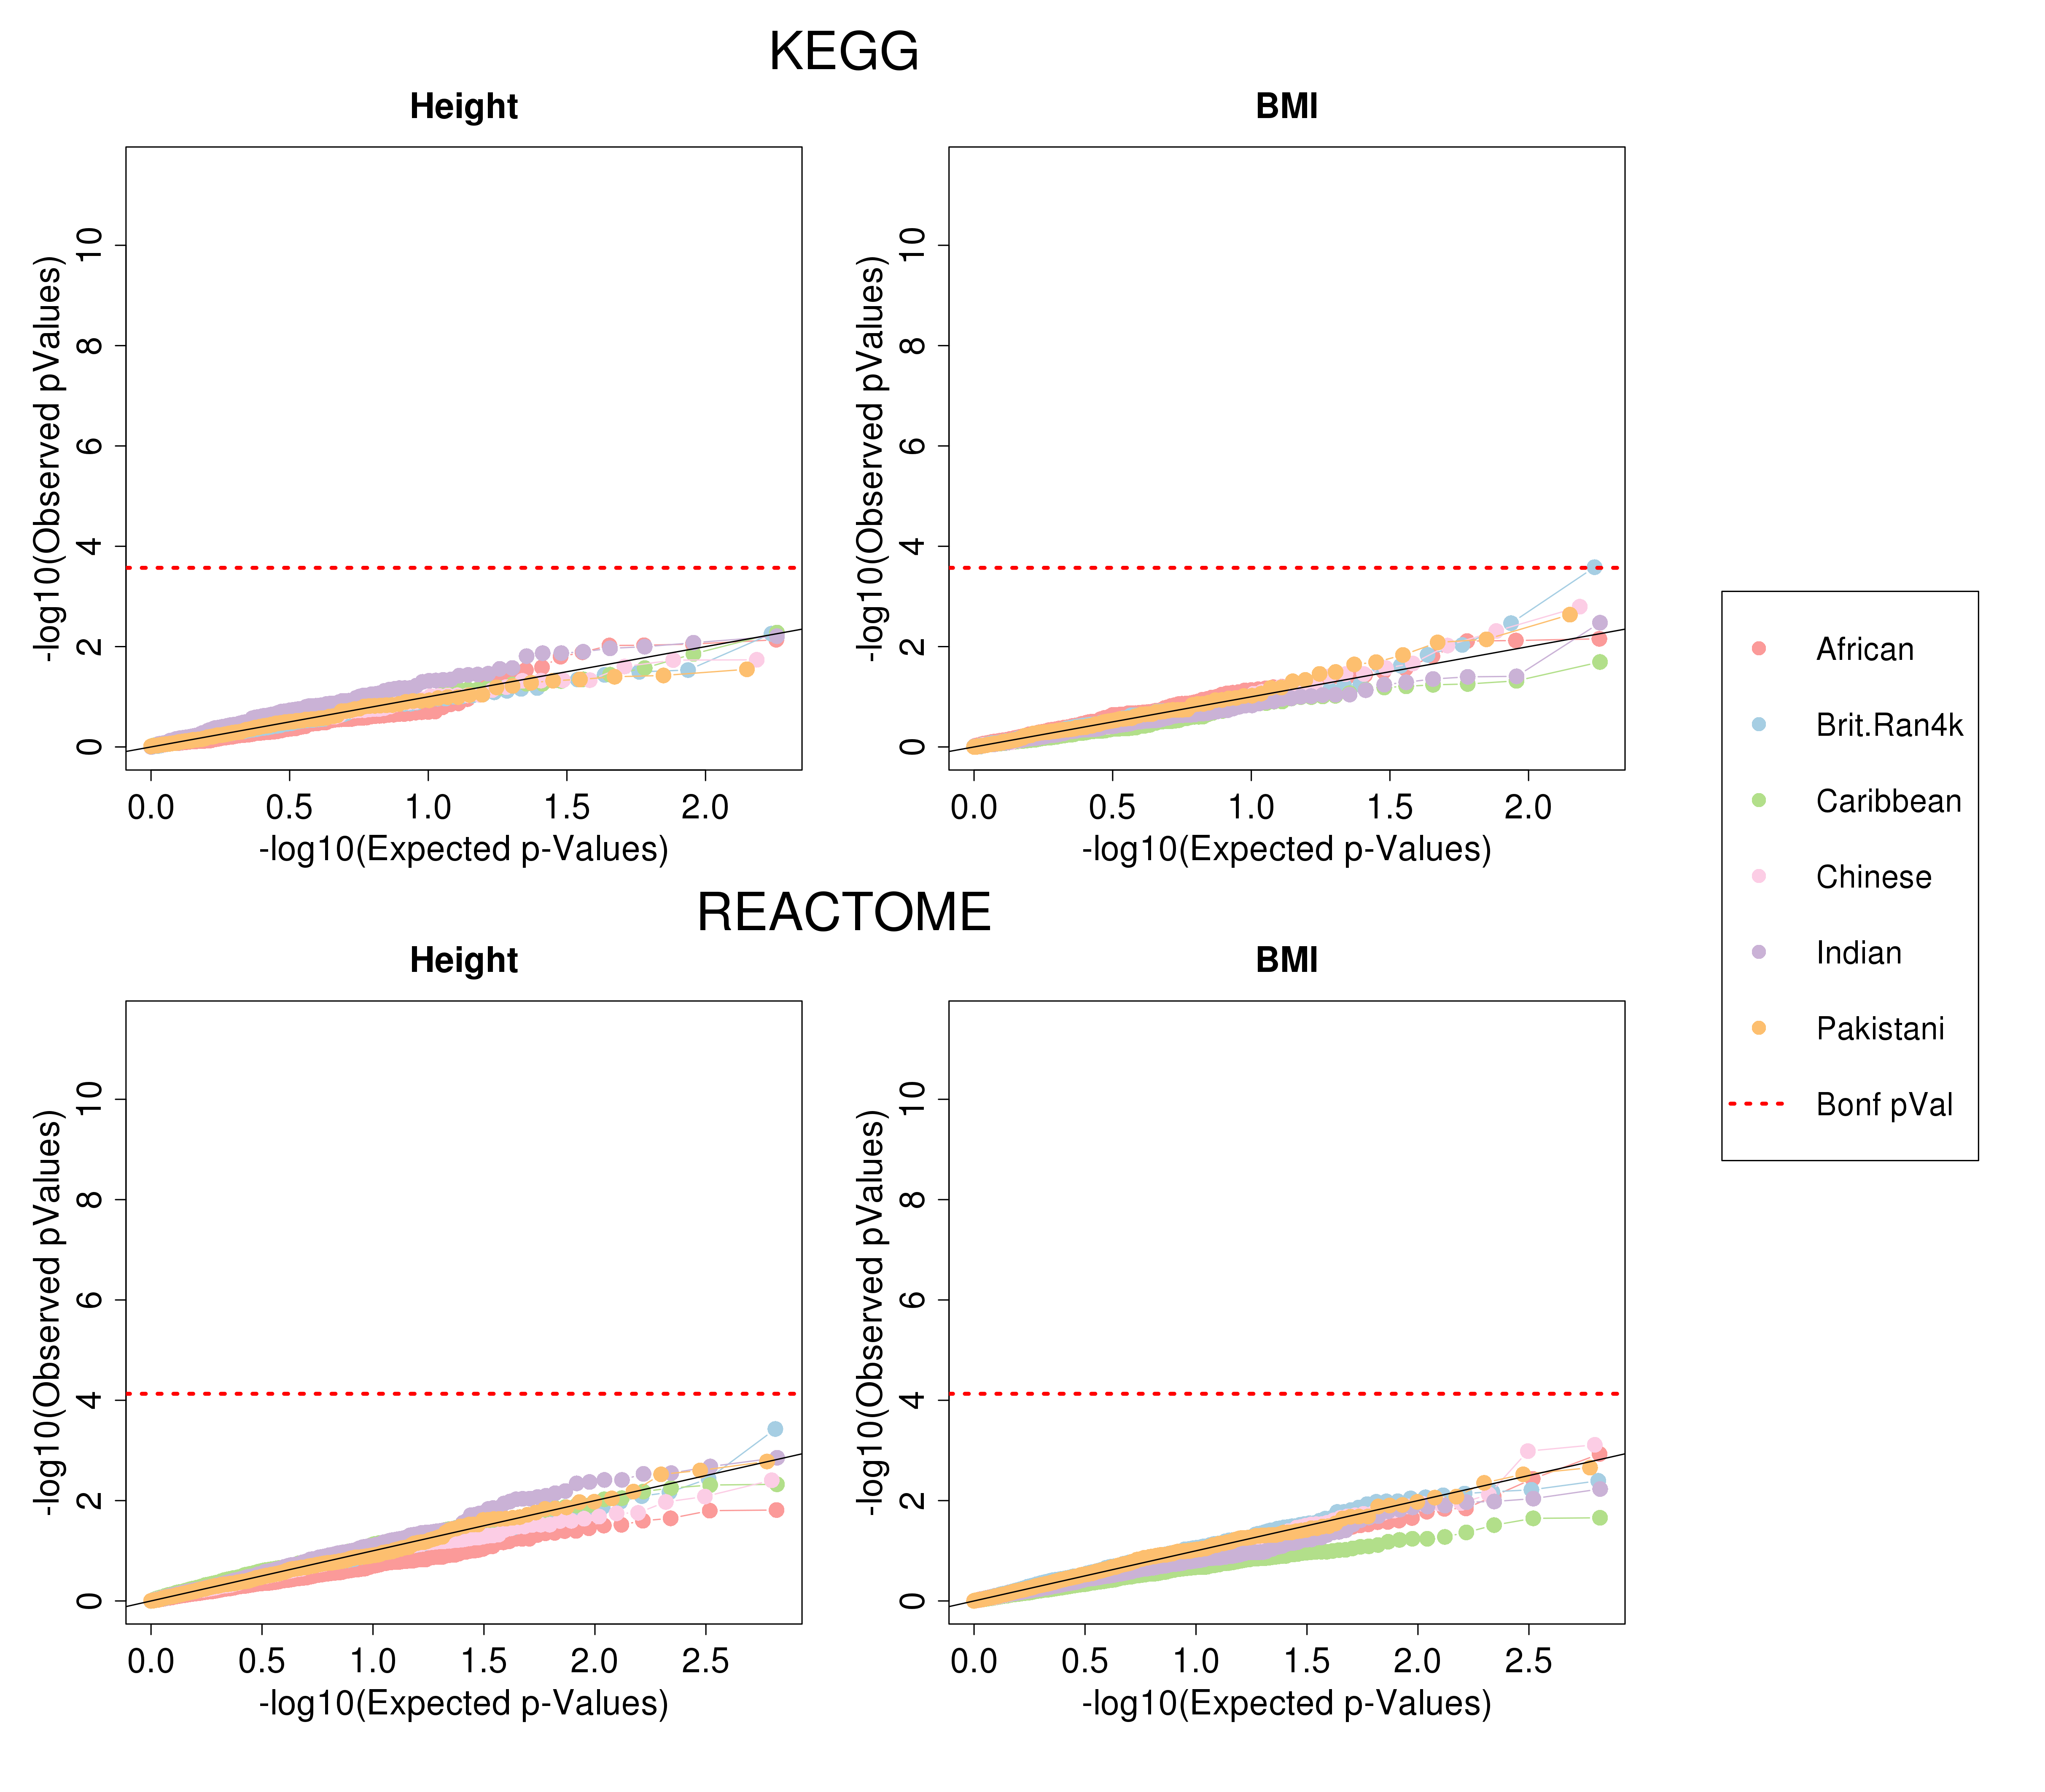
\includegraphics[scale=.35]{Images/Supp/InterPath_Supp_Figure_perm1_QQPlots_AllPaths_vs2.png}
\caption[TBD]{\textbf{QQ-Plots of MAPIT-R results using permuted phenotypes, per subgroup}. The figure shows QQ-plots for running MAPIT-R using a single permutation of either height or BMI measurements within the KEGG and REACTOME databases. Phenotypes were permuted within each population subgroup. Shown on the $x$-axis are the -$\log_{10}$ of the expected $p$-values and the on the $y$-axis are on the -$\log_{10}$ of the observed $p$-values. The dotted red line is the Bonferroni-corrected $p$-value threshold based on the number of pathways tested per pathway database-phenotype combination (Supplementary Table \ref{InterPath-Supp-Table-UKBPopStats}). Looking in total across the ten permutation runs conducted for each pathway database-phenotype-UKB subgroup combination, we find that MAPIT-R properly controls for the false positive rate at varying significance cutoff thresholds (Supplementary Figure \ref{InterPath-Supp-Table-BritReps-FDRs-pt1}).}
\label{InterPath-Supp-Figure-perm1-QQPlots-AllPaths}
\end{figure}
\clearpage

\setlength{\footskip}{3cm}
\begin{figure}[htbp]
\centering
\vspace*{-2cm}
\includegraphics[scale=.2]{Images/Supp/InterPath_Supp_Figure_pValHists_vs3.png}
\caption[TBD]{\textbf{$p$-Value histograms of MAPIT-R results using permuted phenotypes, per subgroup}. The figure shows histograms of MAPIT-R $p$-values collected across ten independent phenotype permutation runs for each UKB subgroup (Supplementary Table \ref{InterPath-Supp-Table-UKBPopStats}). The same phenotype permutation for a given subgroup was used across both pathway databases (i.e. 10 permutations were done for height and 10 done for BMI for each subgroup). And the same covariates used per individual from the original MAPIT-R analysis were used for these permuted-phenotype analyses (see Materials and Methods).}
\label{InterPath-Supp-Figure-10perms-pValHists}
\end{figure}
\clearpage
\setlength{\footskip}{1cm}

\setlength{\footskip}{1cm}
\begin{figure}[htbp]
\centering
\vspace*{-2cm}
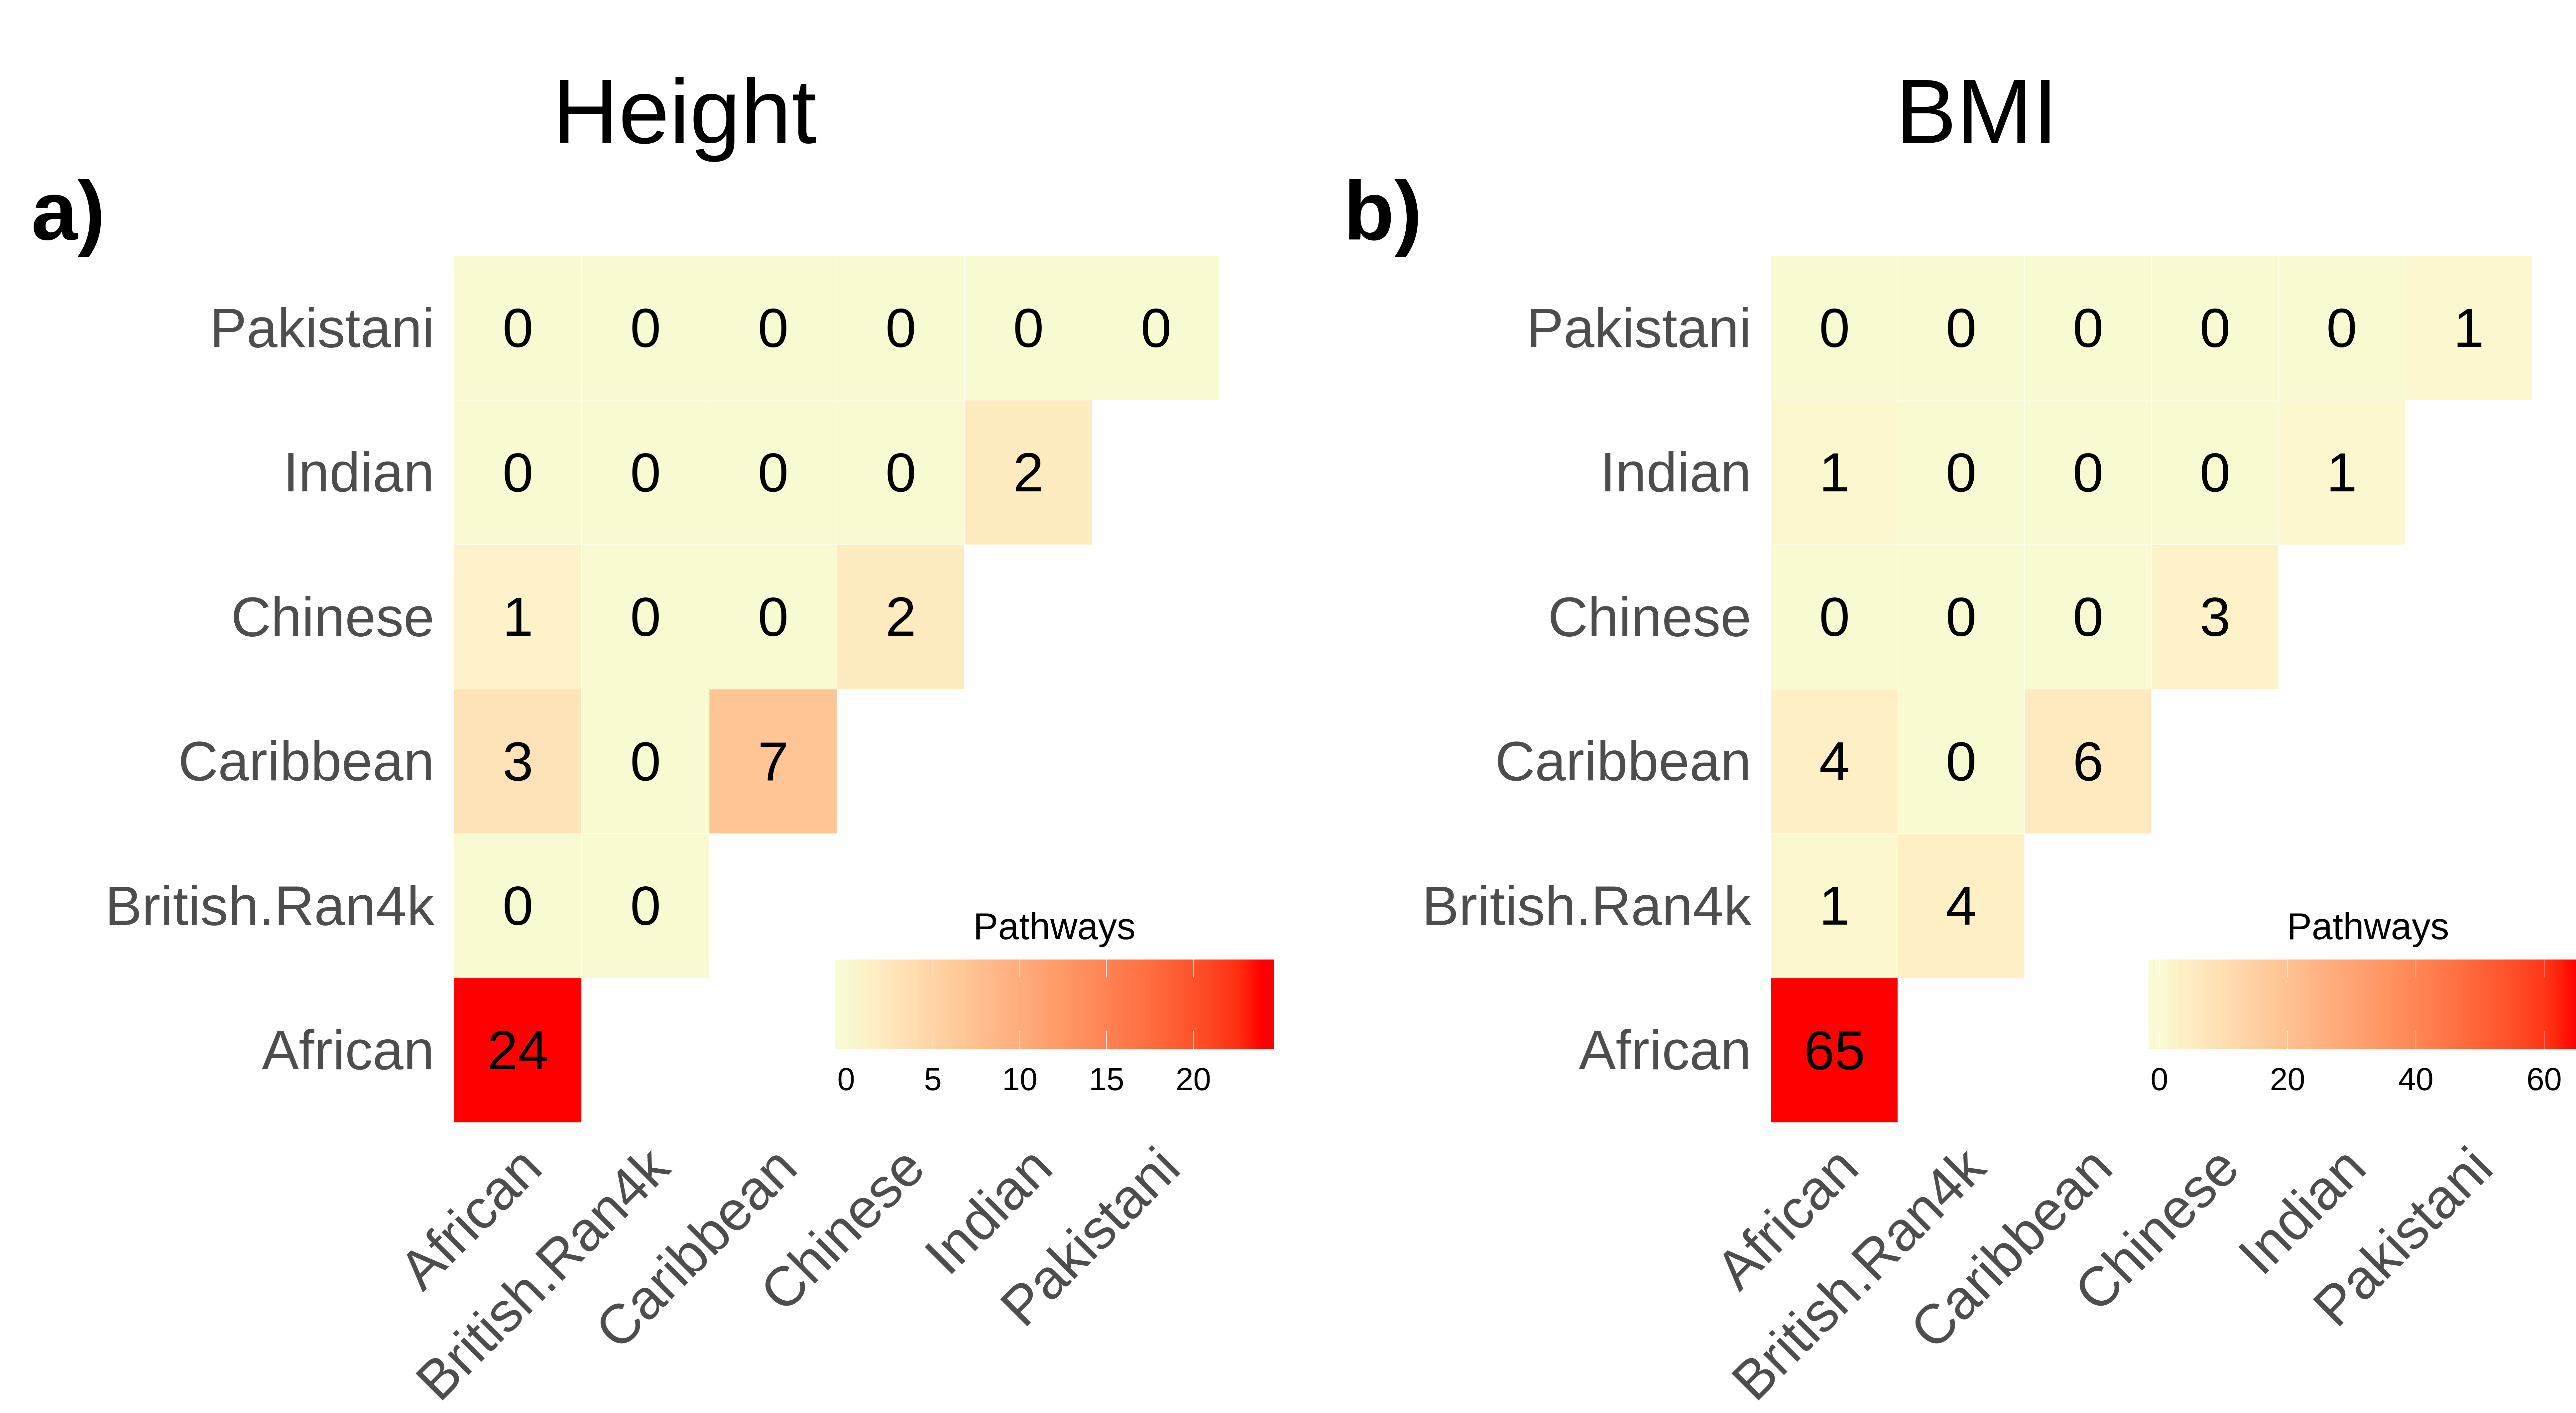
\includegraphics[scale=.225]{Images/Supp/InterPath_Supp_Figure_Heatplots_REACTOME_vs4.png}
\caption[TBD]{\textbf{Overlap of genome-wide significant MAPIT-R pathways between UKB population subgroups: REACTOME}. The heatplots show the numbers of genome-wide significant MAPIT-R pathways that overlap between each UKB subgroup for (a) height and (b) BMI in the REACTOME database. The diagonal shows the total number of genome-wide significant pathways per population subgroup. We observe that most subgroups often have overlap with the African subgroup but rarely do so with the remaining non-African subgroups. For results from the KEGG database see Figure \ref{InterPath-Main-Figure-Heatplots-KEGG}.}
\label{InterPath-Supp-Figure-Heatplots-REACTOME}
\end{figure}
\clearpage
\setlength{\footskip}{1cm}

\setlength{\footskip}{3cm}
\begin{figure}[htbp]
\centering
\vspace*{-2cm}
\includegraphics[scale=.2]{Images/Supp/InterPath_Supp_Figure_MAPITR_PhenoComps_AllPops_vs4.png}
\caption[TBD]{\textbf{Comparison of MAPIT-R results between height and BMI, per subgroup}. The figure shows MAPIT-R height results plotted against MAPIT-R BMI results for all pathways from the KEGG and REACTOME databases in all UKB subgroups. The $x$-axes are the MAPIT-R height -$\log_{10}$ $p$-values and the $y$-axes are the MAPIT-R BMI -$\log_{10}$ $p$-values. The dotted red lines are the Bonferroni-corrected $p$-value thresholds for genome-wide significance in each pathway-phenotype-subgroup combination. The correlation between the phenotype -$\log_{10}$ $p$-values is shown in the bottom right.}
\label{InterPath-Supp-Figure-MAPITR-PhenoComps-AllPops}
\end{figure}
\clearpage
\setlength{\footskip}{1cm}

\begin{figure}[htbp]
\centering
\hspace*{-1.75cm}
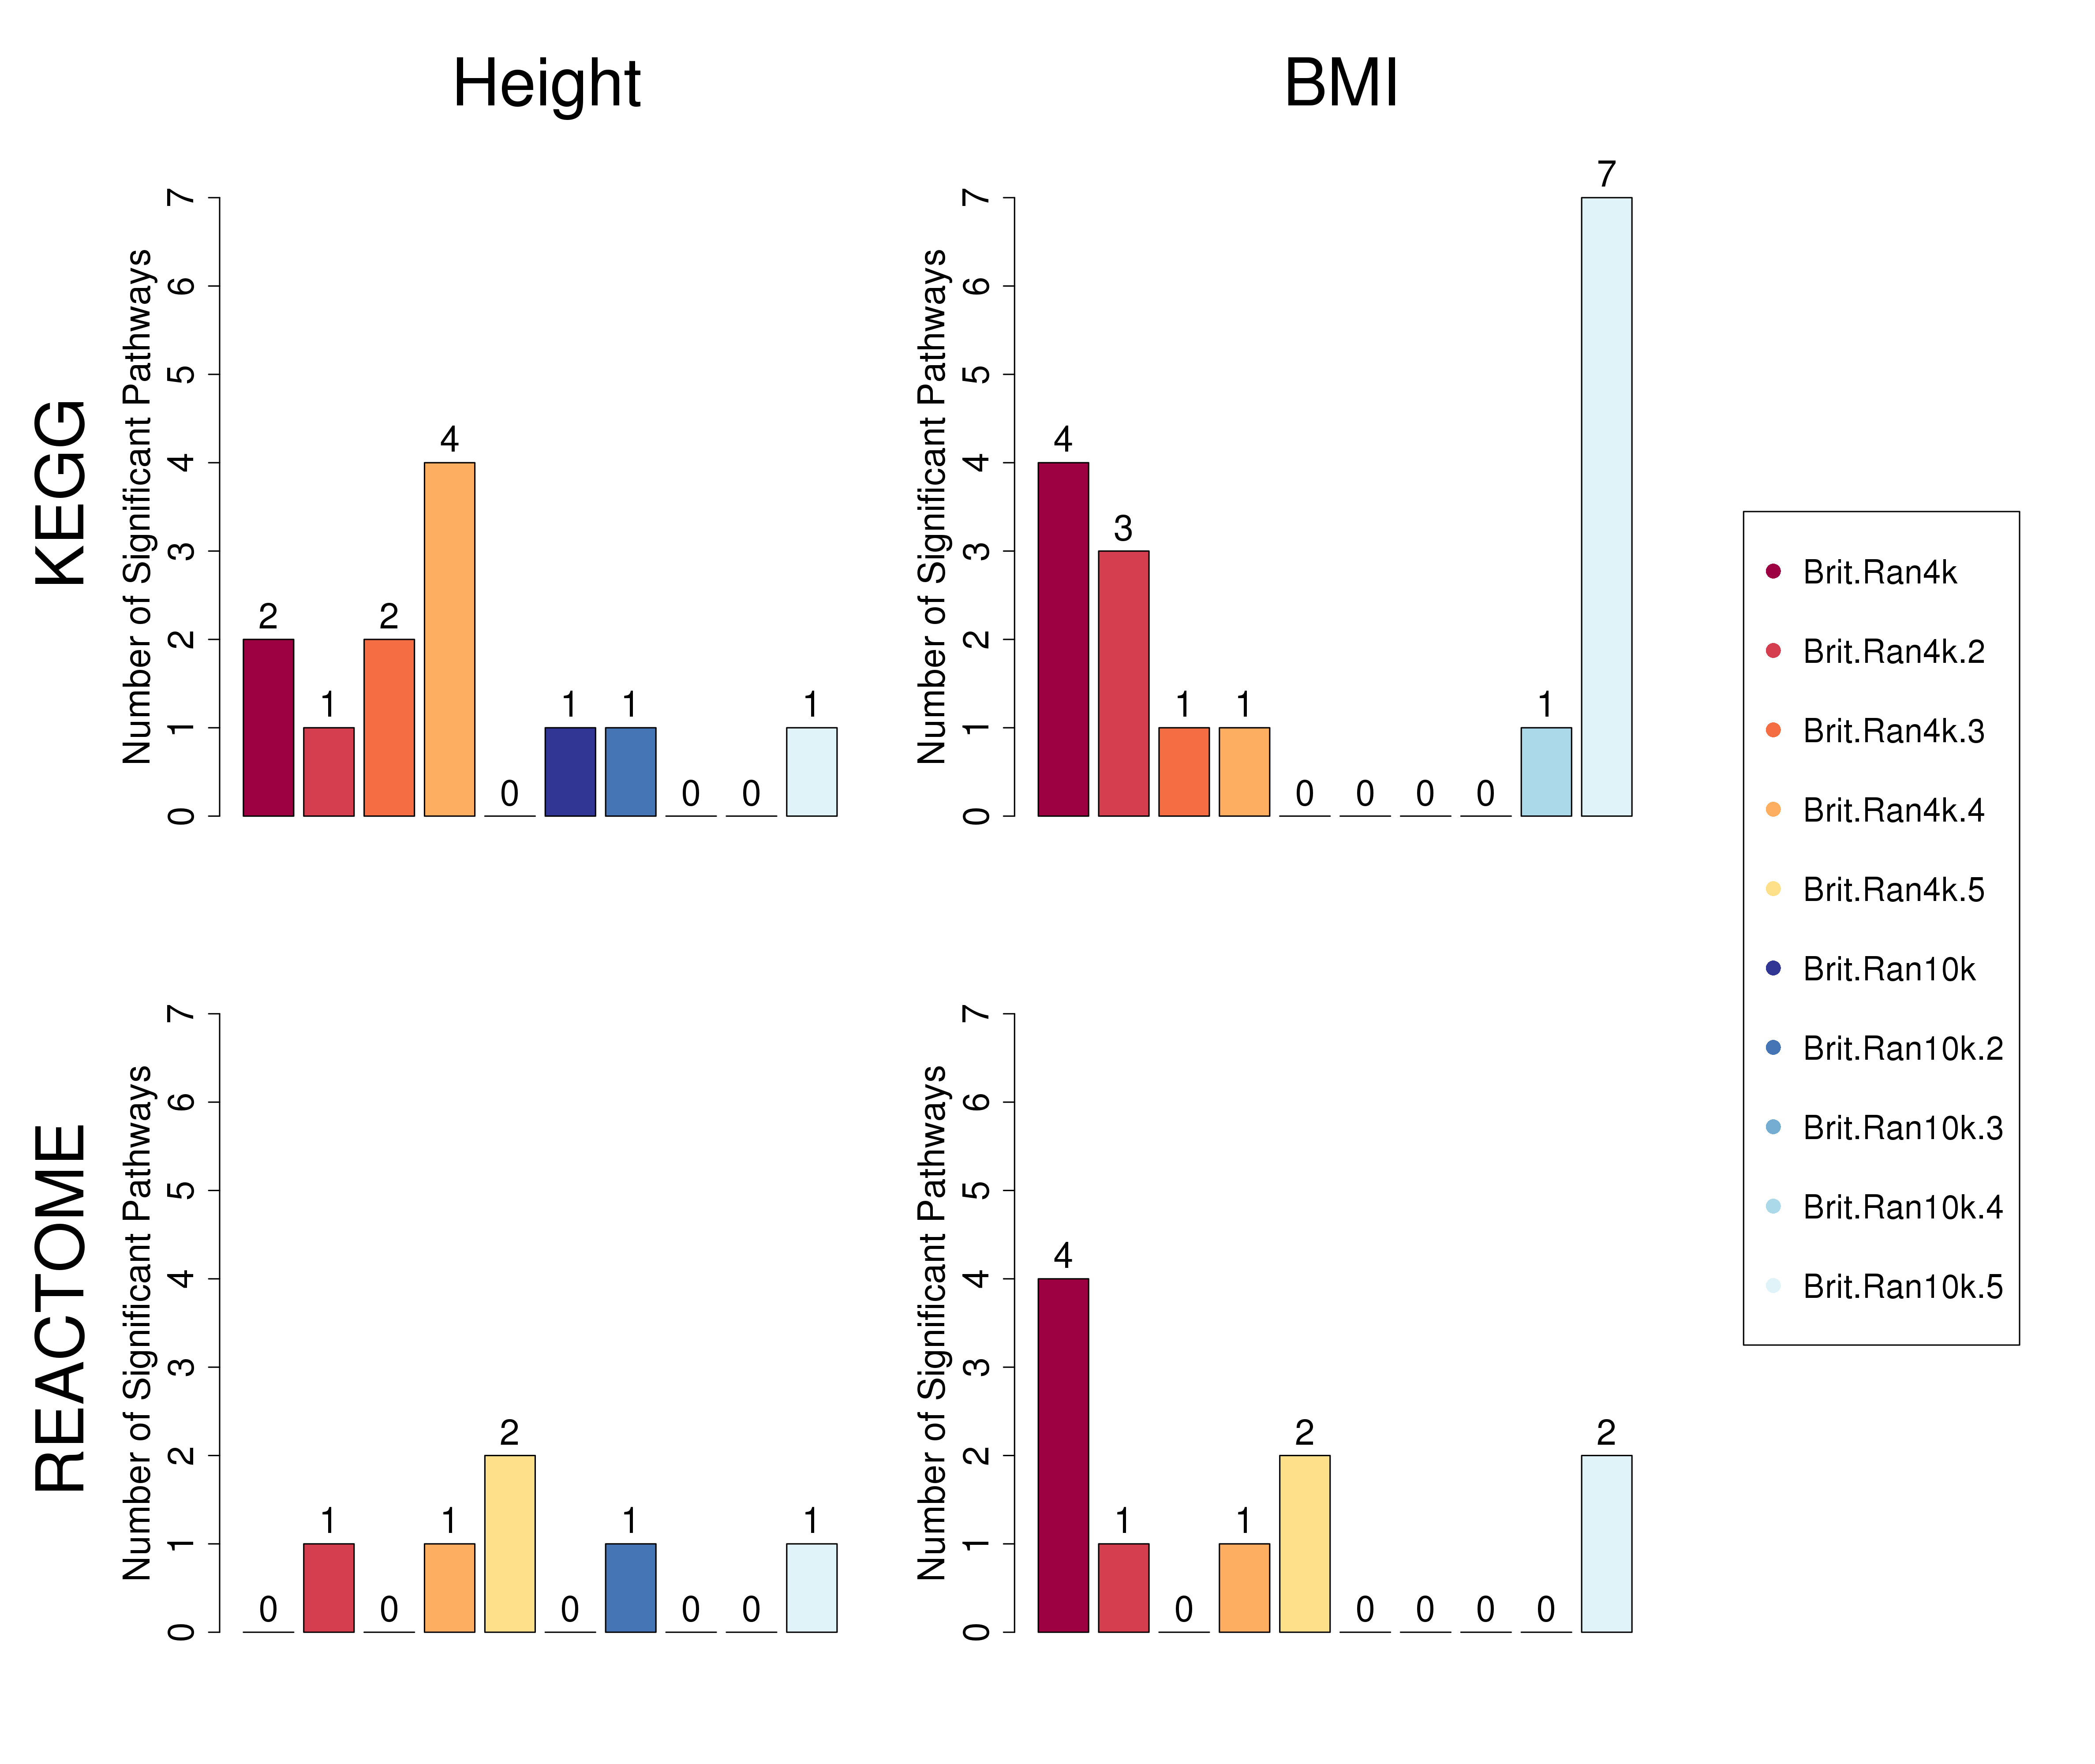
\includegraphics[scale=.45]{Images/Supp/InterPath_Supp_Figure_BritReps_Barplot_vs4.png}
\caption[TBD]{\textbf{Numbers of pathways that have significant marginal epistasis, per British replicate}. The barplots show the number of genome-wide significant pathways found from running MAPIT-R for both height and BMI in the KEGG and REACTOME databases on each of the British subsample replicate subgroups we analyzed. Genome-wide significance was determined by using Bonferroni-corrected $p$-value thresholds based on the number of pathways tested in each pathway database-phenotype-subgroup combination. Most replicate runs did not produce many significant results.}
\label{InterPath-Supp-Figure-BritReps-Barplots}
\end{figure}
\clearpage

\newcounter{CharNumber4}
\setcounter{CharNumber4}{1}
\renewcommand{\thefigure}{\arabic{figure}\alph{CharNumber4}}
\begin{landscape}
\begin{figure}[htbp]
\centering
\includegraphics[scale=.2]{Images/Supp/InterPath_Supp_Figure_BritReps_Heatplots_KEGG_vs4.png}
\caption[TBD]{\textbf{Overlap of genome-wide significant MAPIT-R pathways between British replicate subgroups: KEGG}. The heatplots show the numbers of genome-wide significant MAPIT-R pathways that overlap between each British replicate subgroup for (a) height and (b) BMI in the KEGG database. The diagonal shows the total number of genome-wide significant pathways per population subgroup. We do not observe many genome-wide significant pathways or pathways that overlap between replicate subgroups.}
\label{InterPath-Supp-Figure-BritReps-Heatplots-AllPaths-KEGG}
\end{figure}
\clearpage
\addtocounter{figure}{-1}
\addtocounter{CharNumber4}{1}
\end{landscape}

\begin{landscape}
\begin{figure}[htbp]
\centering
\includegraphics[scale=.2]{Images/Supp/InterPath_Supp_Figure_BritReps_Heatplots_REACTOME_vs4.png}
\caption[TBD]{\textbf{Overlap of genome-wide significant MAPIT-R pathways between British replicate subgroups: REACTOME}. The heatplots show the numbers of genome-wide significant MAPIT-R pathways that overlap between each British replicate subgroup for (a) height and (b) BMI in the REACTOME database. The diagonal shows the total number of genome-wide significant pathways per population subgroup. We do not observe many genome-wide significant pathways or pathways that overlap between replicate subgroups.}
\label{InterPath-Supp-Figure-BritReps-Heatplots-AllPaths-REACTOME}
\end{figure}
\clearpage
\end{landscape}
\renewcommand{\thefigure}{\arabic{figure}}

\begin{figure}[htbp]
\centering
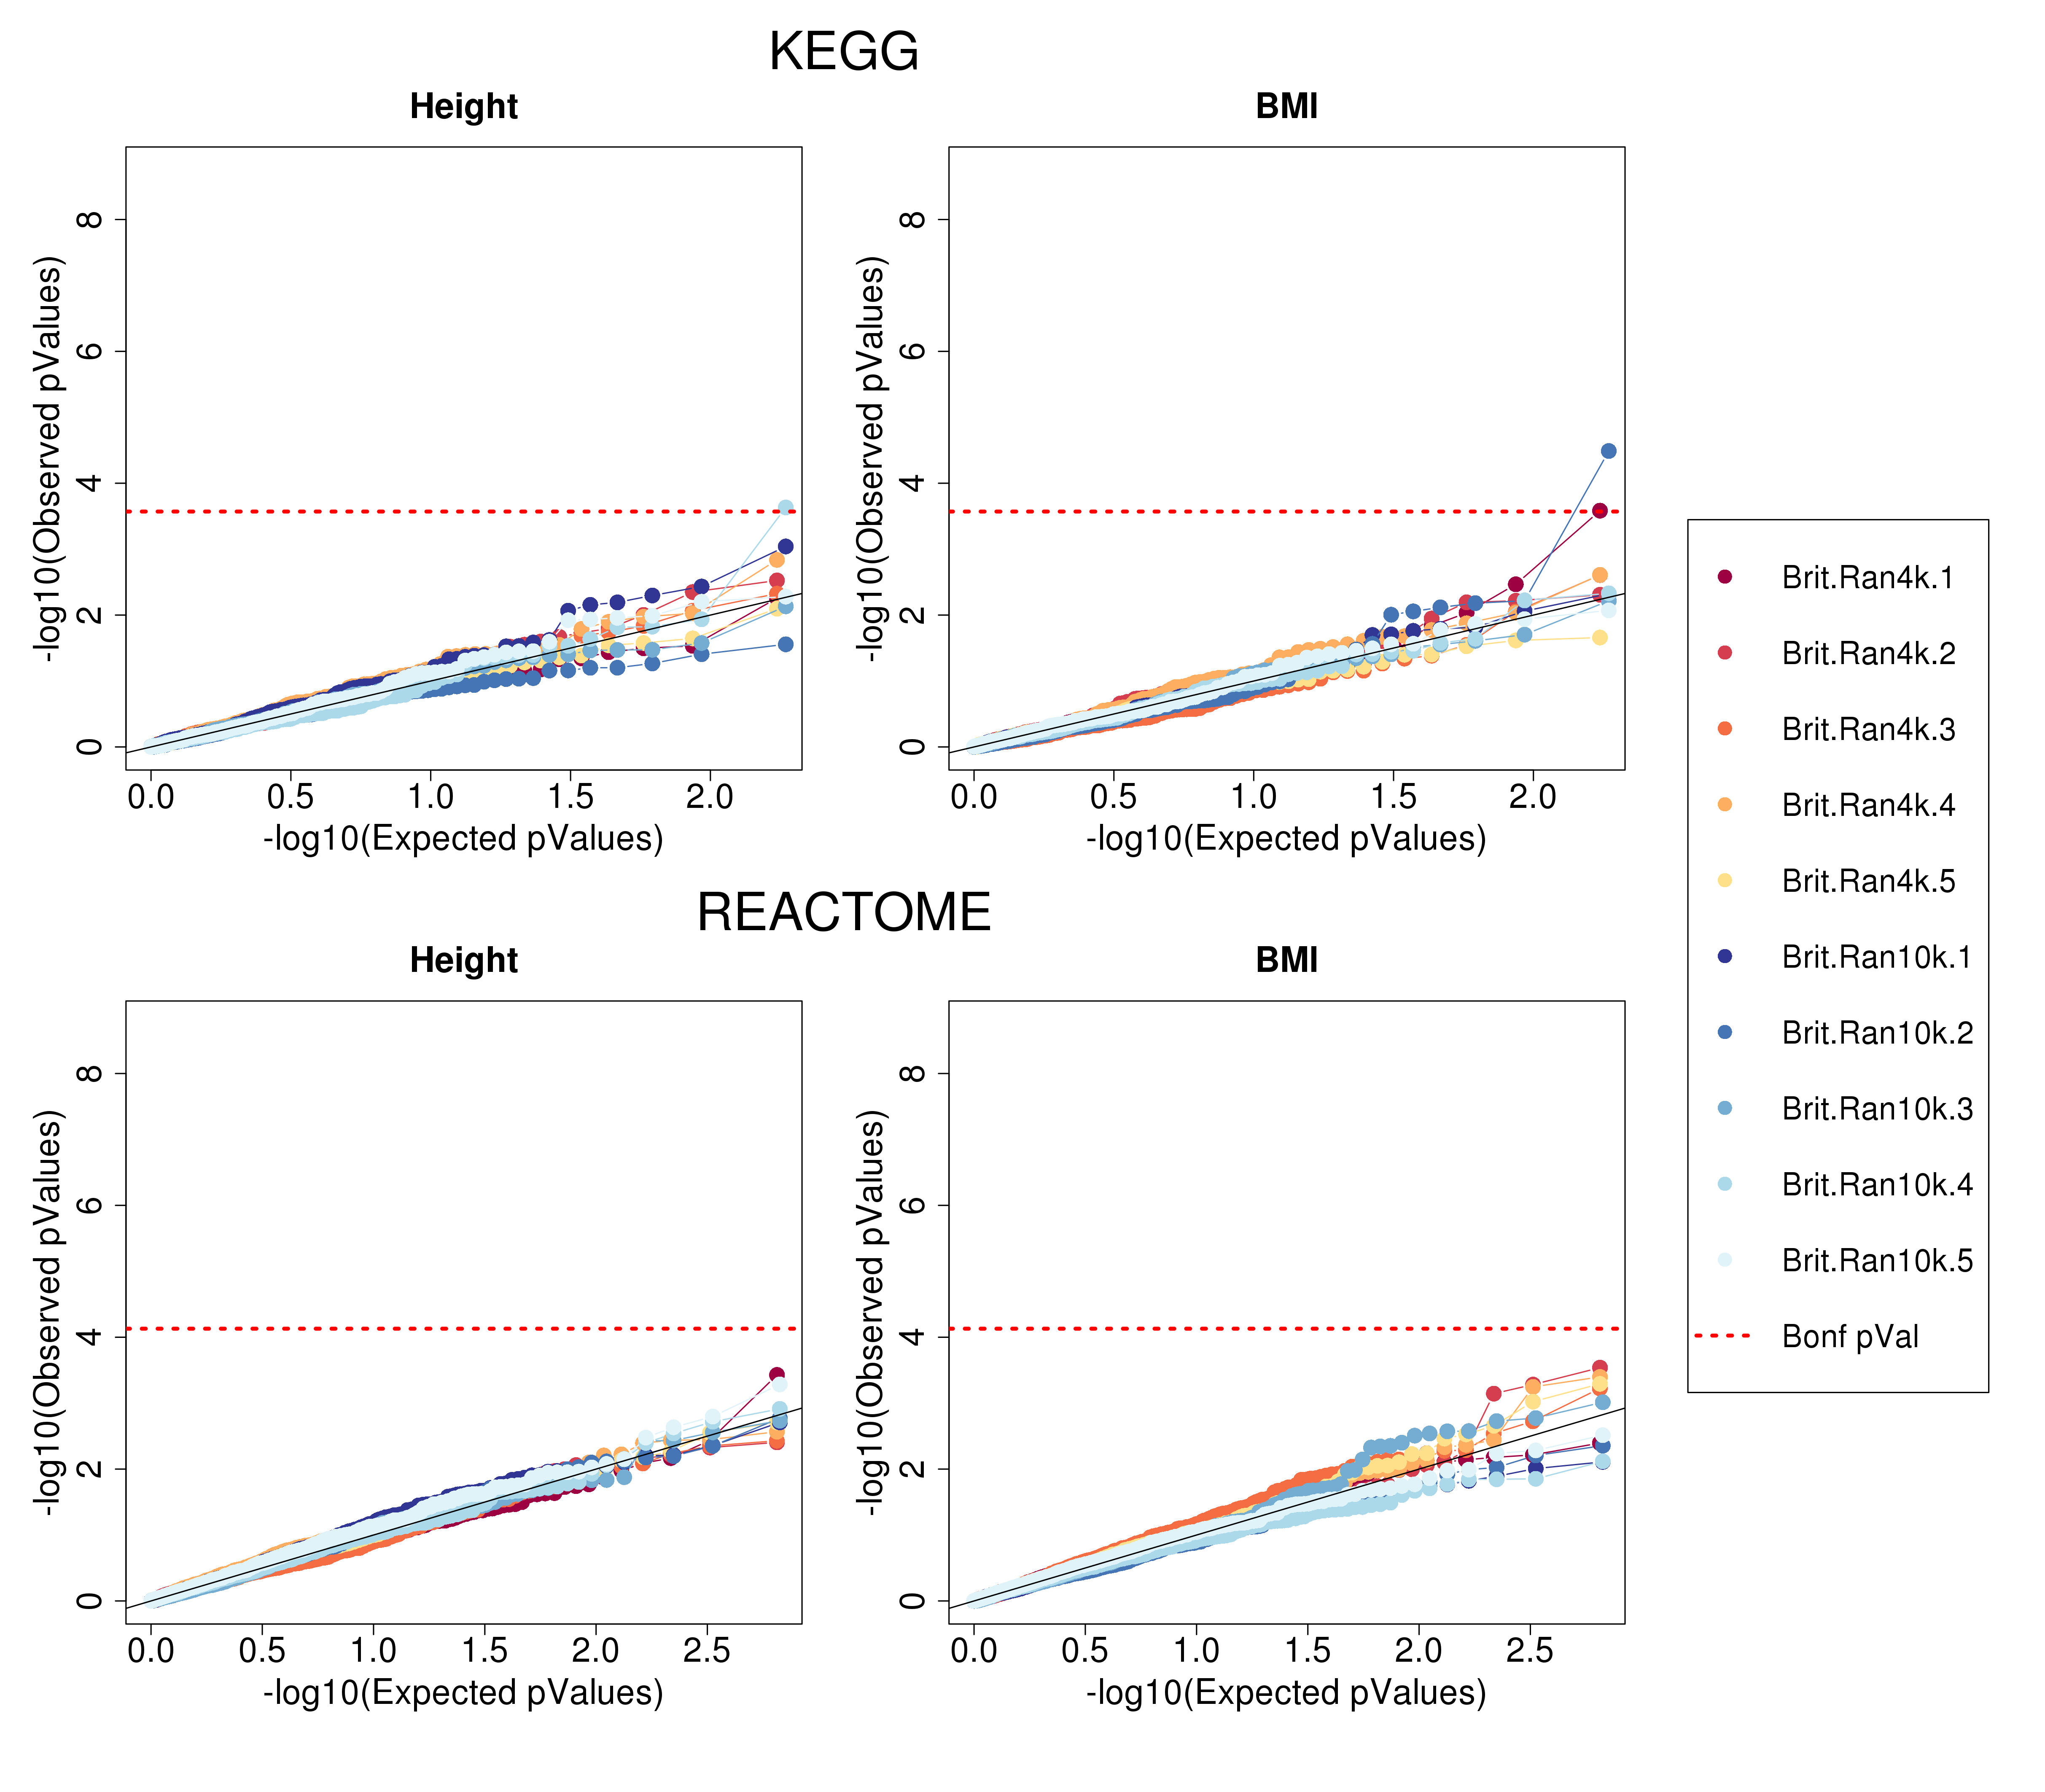
\includegraphics[scale=.35]{Images/Supp/InterPath_Supp_Figure_BritReps_perm1_QQPlots_AllPaths_vs1.png}
\caption[TBD]{\textbf{QQ-Plots of MAPIT-R results using permuted phenotypes, per British replicate}. The figure shows QQ-plots for running MAPIT-R using single, permuted versions of both height and BMI with the KEGG \& REACTOME databases. Phenotypes were permuted within each British replicate subgroup. Shown on the $x$-axis are the -$\log_{10}$ of the expected $p$-values and the on the $y$-axis are on the -$\log_{10}$ of the observed $p$-values. The dotted red line is the Bonferroni-corrected $p$-value threshold based on the number of pathways tested per pathway database-phenotype combination. We find across all pathway database-phenotype-replicate combinations that MAPIT-R continues to show proper null behavior within the range expected when using permuted phenotypes.}
\label{InterPath-Supp-Figure-BritReps-perm1-QQPlots-AllPaths}
\end{figure}
\clearpage

%\newcounter{CharNumber3}
%\setcounter{CharNumber3}{1}
%\renewcommand{\thefigure}{\arabic{figure}\alph{CharNumber3}}
\setlength{\footskip}{1cm}
\begin{figure}[htbp]
\centering
\vspace*{-1cm}
\includegraphics[scale=.2]{Images/Supp/InterPath_Supp_Figure_BritReps_pValHists_AllPaths_vs1_pt1.png}
\caption[TBD]{\textbf{$p$-Value histograms of MAPIT-R results using permuted phenotypes, per British replicate}. The figure shows histograms of MAPIT-R $p$-values collected across ten independent phenotype permutation runs for each British Ran4000 and Ran10000 subsample replicate. The same phenotype permutation for a given replicate was used across both pathway databases (i.e. 10 permutations were done for height and 10 done for BMI for each subgroup). Covariates used from the original MAPIT-R analysis were kept the same.}
\label{InterPath-Supp-Figure-BritReps-10perms-pValHists-pt1}
\end{figure}
\clearpage
\setlength{\footskip}{1cm}
\addtocounter{figure}{-1}
%\addtocounter{CharNumber3}{1}

\setlength{\footskip}{2cm}
\begin{figure}[htbp]
\centering
\vspace*{-1cm}
\includegraphics[scale=.2]{Images/Supp/InterPath_Supp_Figure_BritReps_pValHists_AllPaths_vs1_pt2.png}
\caption[TBD]{\textbf{$p$-Value histograms of MAPIT-R results using permuted phenotypes, per British replicate}. The figure shows histograms of MAPIT-R $p$-values collected across ten independent phenotype permutation runs for each British Ran4000 and Ran10000 subsample replicate. The same phenotype permutation for a given replicate was used across both pathway databases (i.e. 10 permutations were done for height and 10 done for BMI for each subgroup). Covariates used from the original MAPIT-R analysis were kept the same.}
\label{InterPath-Supp-Figure-BritReps-10perms-pValHists-pt2}
\end{figure}
\clearpage
\setlength{\footskip}{1cm}
%\renewcommand{\thefigure}{\arabic{figure}}

\setlength{\footskip}{3cm}
\begin{figure}[htbp]
\centering
\vspace*{-2cm}
\includegraphics[scale=.2]{Images/Supp/InterPath_Supp_Figure_pValsVsNumSNPs_vs3.png}
\caption[TBD]{\textbf{Number of SNPs in a pathway versus a pathway's MAPIT-R $p$-value}. Caption continued on next page.}
\label{InterPath-Supp-Figure-pValsVsNumSNPs}
\end{figure}
\clearpage
\setlength{\footskip}{1cm}

\addtocounter{figure}{-1}
\begin{figure} [t!]
  \caption{\textbf{Number of SNPs in a pathway versus a pathway's MAPIT-R $p$-value}. The figure shows plots comparing the MAPIT-R $p$-values from our main analysis to the number of SNPs present in each pathway. Results for every pathway database-phenotype-UB subgroup combinations are shown. The dotted red line is the line of best fit and the legend provides the regression coefficient and its associated $p$-value. We observe that for most combinations there is a significant relationship between MAPIT-R $p$-value and the number of SNPs present in a pathway. This follows our hypothesis that combining SNPs together in a joint analysis might provide greater power to detect marginal epistasis than analyzing each SNP independently. We note, however, that these results appear to not solely be driven just by the presence or absence of large SNP counts -- conducting this same analysis on one of our sets of permuted phenotypes we now find very few significant relationships between MAPIT-R $p$-values and pathway SNP counts (Supplementary Figure \ref{InterPath-Supp-Figure-pValsVsNumSNPs-perm1}).}
\label{InterPath-Supp-Figure-pValsVsNumSNPs-Caption}
\end{figure}
\clearpage

\setlength{\footskip}{3cm}
\begin{figure}[htbp]
\centering
\vspace*{-2cm}
\includegraphics[scale=.2]{Images/Supp/InterPath_Supp_Figure_pValsVsNumSNPs_perm1_vs3.png}
\caption[TBD]{\textbf{Number of SNPs in a pathway versus a pathway's MAPIT-R $p$-value using permuted phenotypes}. Caption continued on next page.}
\label{InterPath-Supp-Figure-pValsVsNumSNPs-perm1}
\end{figure}
\clearpage
\setlength{\footskip}{1cm}

\addtocounter{figure}{-1}
\begin{figure} [t!]
  \caption{\textbf{Number of SNPs in a pathway versus a pathway's MAPIT-R $p$-value using permuted phenotypes}. The figure shows plots comparing the MAPIT-R $p$-values from our main analysis to the number of SNPs present in each pathway. For this analysis a single set of our permuted phenotypes (i.e. Supplementary Figure \ref{InterPath-Supp-Figure-perm1-QQPlots-AllPaths}) was used for each UKB subgroup. Results for every pathway database-phenotype-subgroup combination is shown. The dotted red line is the line of best fit and the legend provides the regression coefficient and its associated $p$-value. We observe that for very few combinations there is any relationship between MAPIT-R $p$-value and the number of SNPs present in a pathway. For the same analysis on the original set of observed phenotypes, see Supplementary Figure \ref{InterPath-Supp-Figure-pValsVsNumSNPs}.}
\label{InterPath-Supp-Figure-pValsVsNumSNPs-perm1-Caption}
\end{figure}
\clearpage

%\begin{figure}[htb]
%\centering
%\hspace*{-1.4cm}
%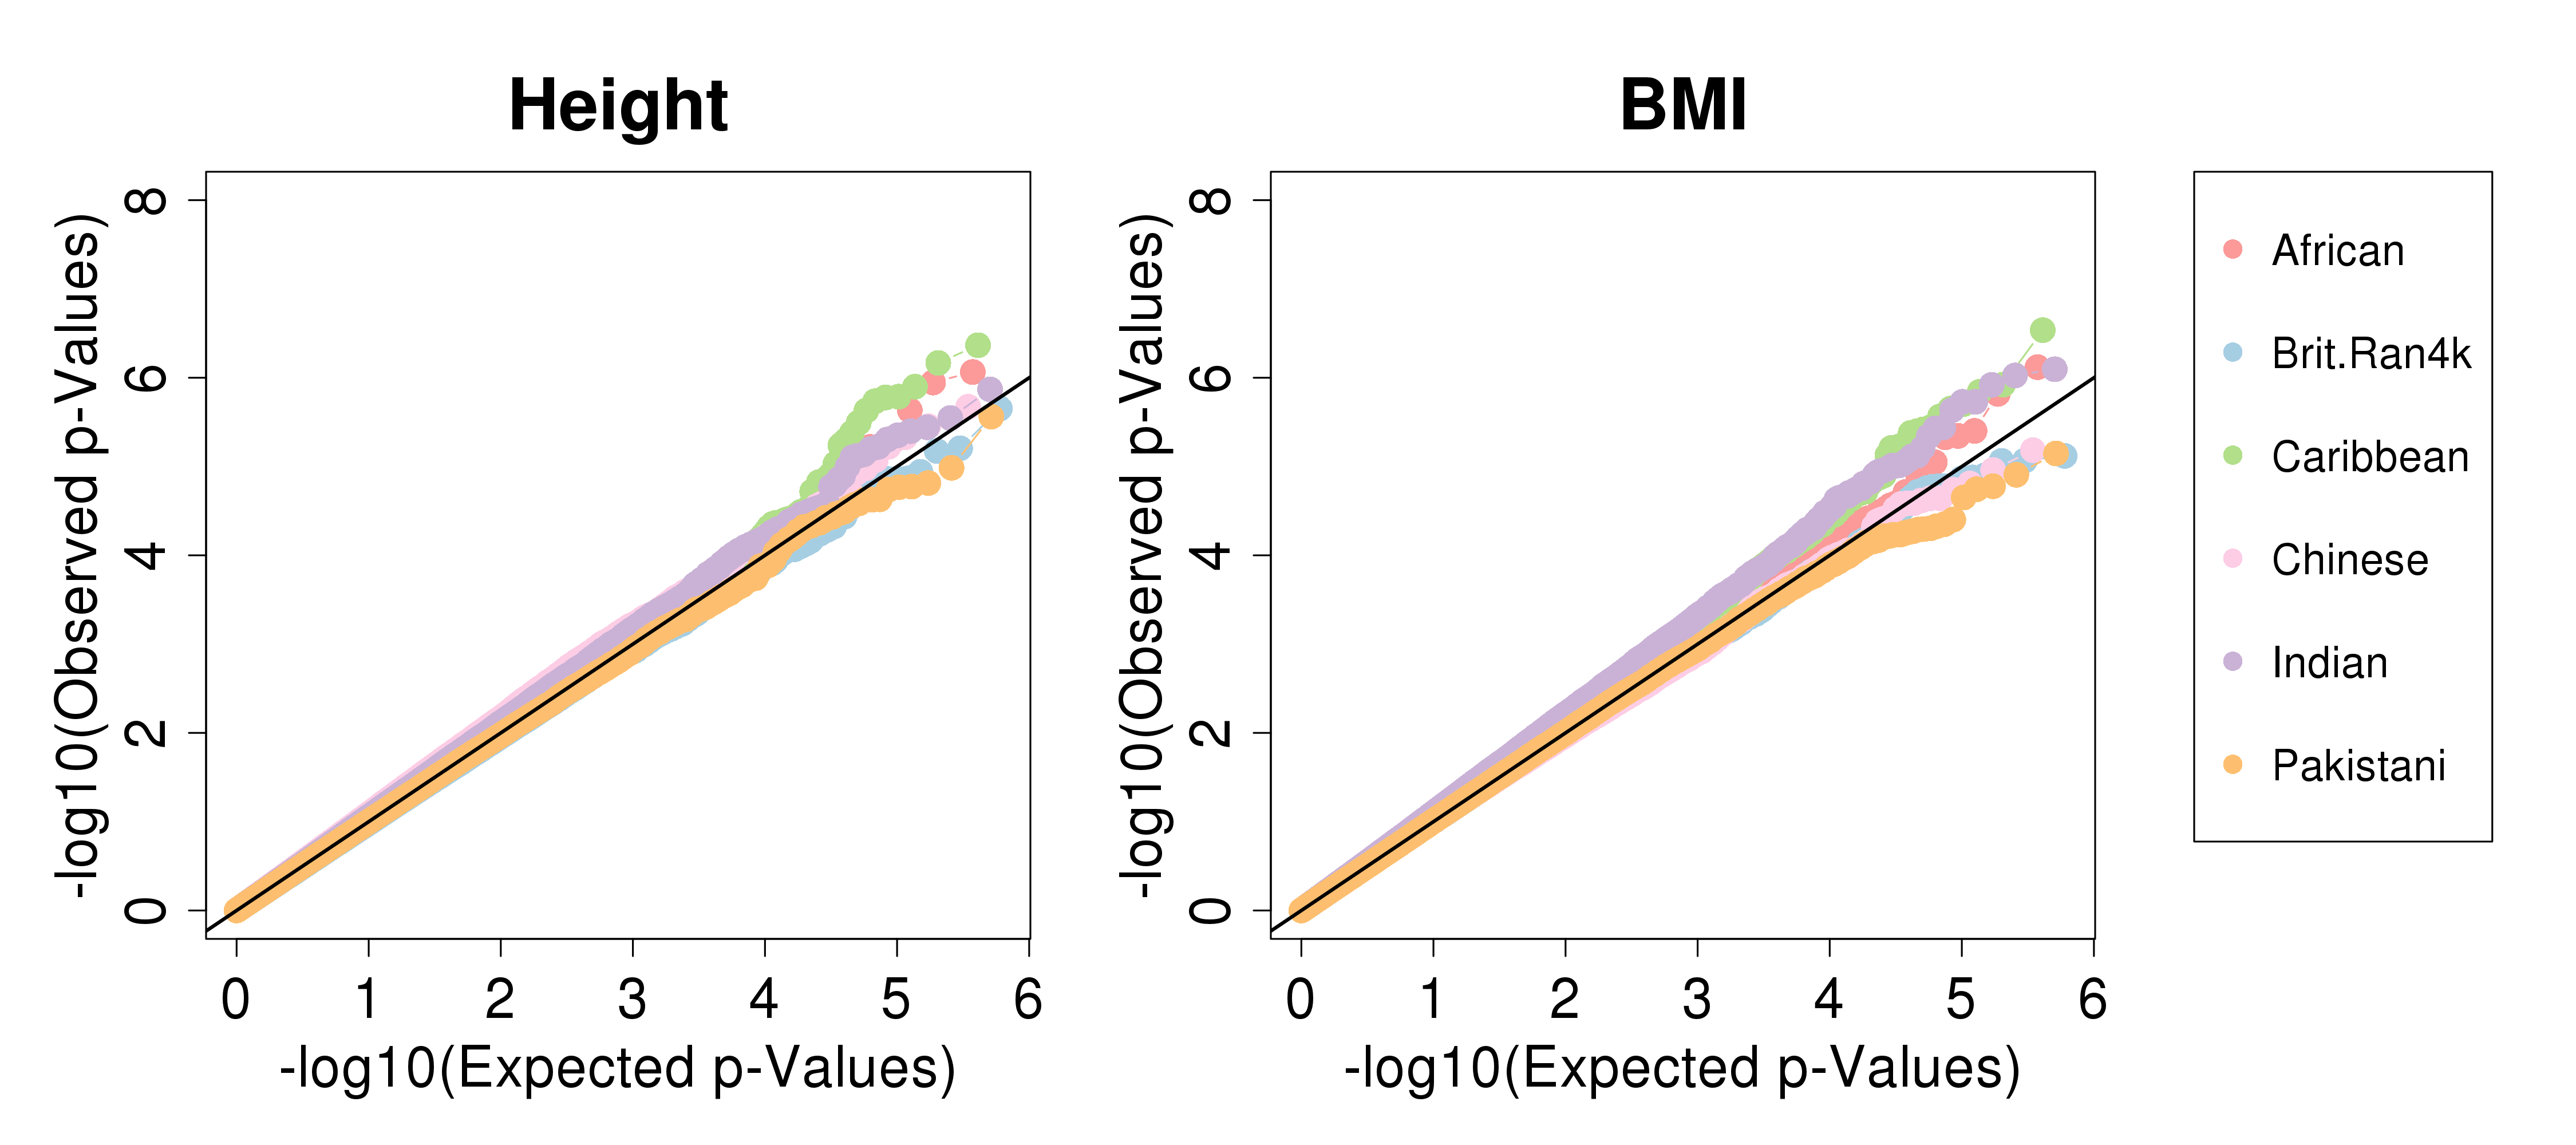
\includegraphics[scale=.45]{Images/Main/InterPath_Main_Figure_MAPIT_vs4_HeightBMI.png}
%\caption[TBD]{\textbf{QQ-Plots of MAPIT results, per subgroup}. The figure shows QQ-plots of our results from running MAPIT on our four initial UKB population subgroups in height and BMI. On the $x$-axis are the -$\log_{10}$ of the expected $p$-values and the on the $y$-axis are on the -$\log_{10}$ of the observed $p$-values. Each data point is a SNP and total SNP counts per UKB subgroup can be found in Supplementary Table \ref{InterPath-Supp-Table-UKBPopStats}. We observe no genome-wide significant signals in any subgroup across both phenotypes ($p$-value $< 5\times10^{-8}$) and, due to this lack of significant results, observe no clear differences in patterns between our subgroups.}
%\label{InterPath-Supp-Figure-MAPIT-HeightBMI}
%\end{figure}

%\begin{figure}[htbp]
%\centering
%\hspace*{-1.7cm}
%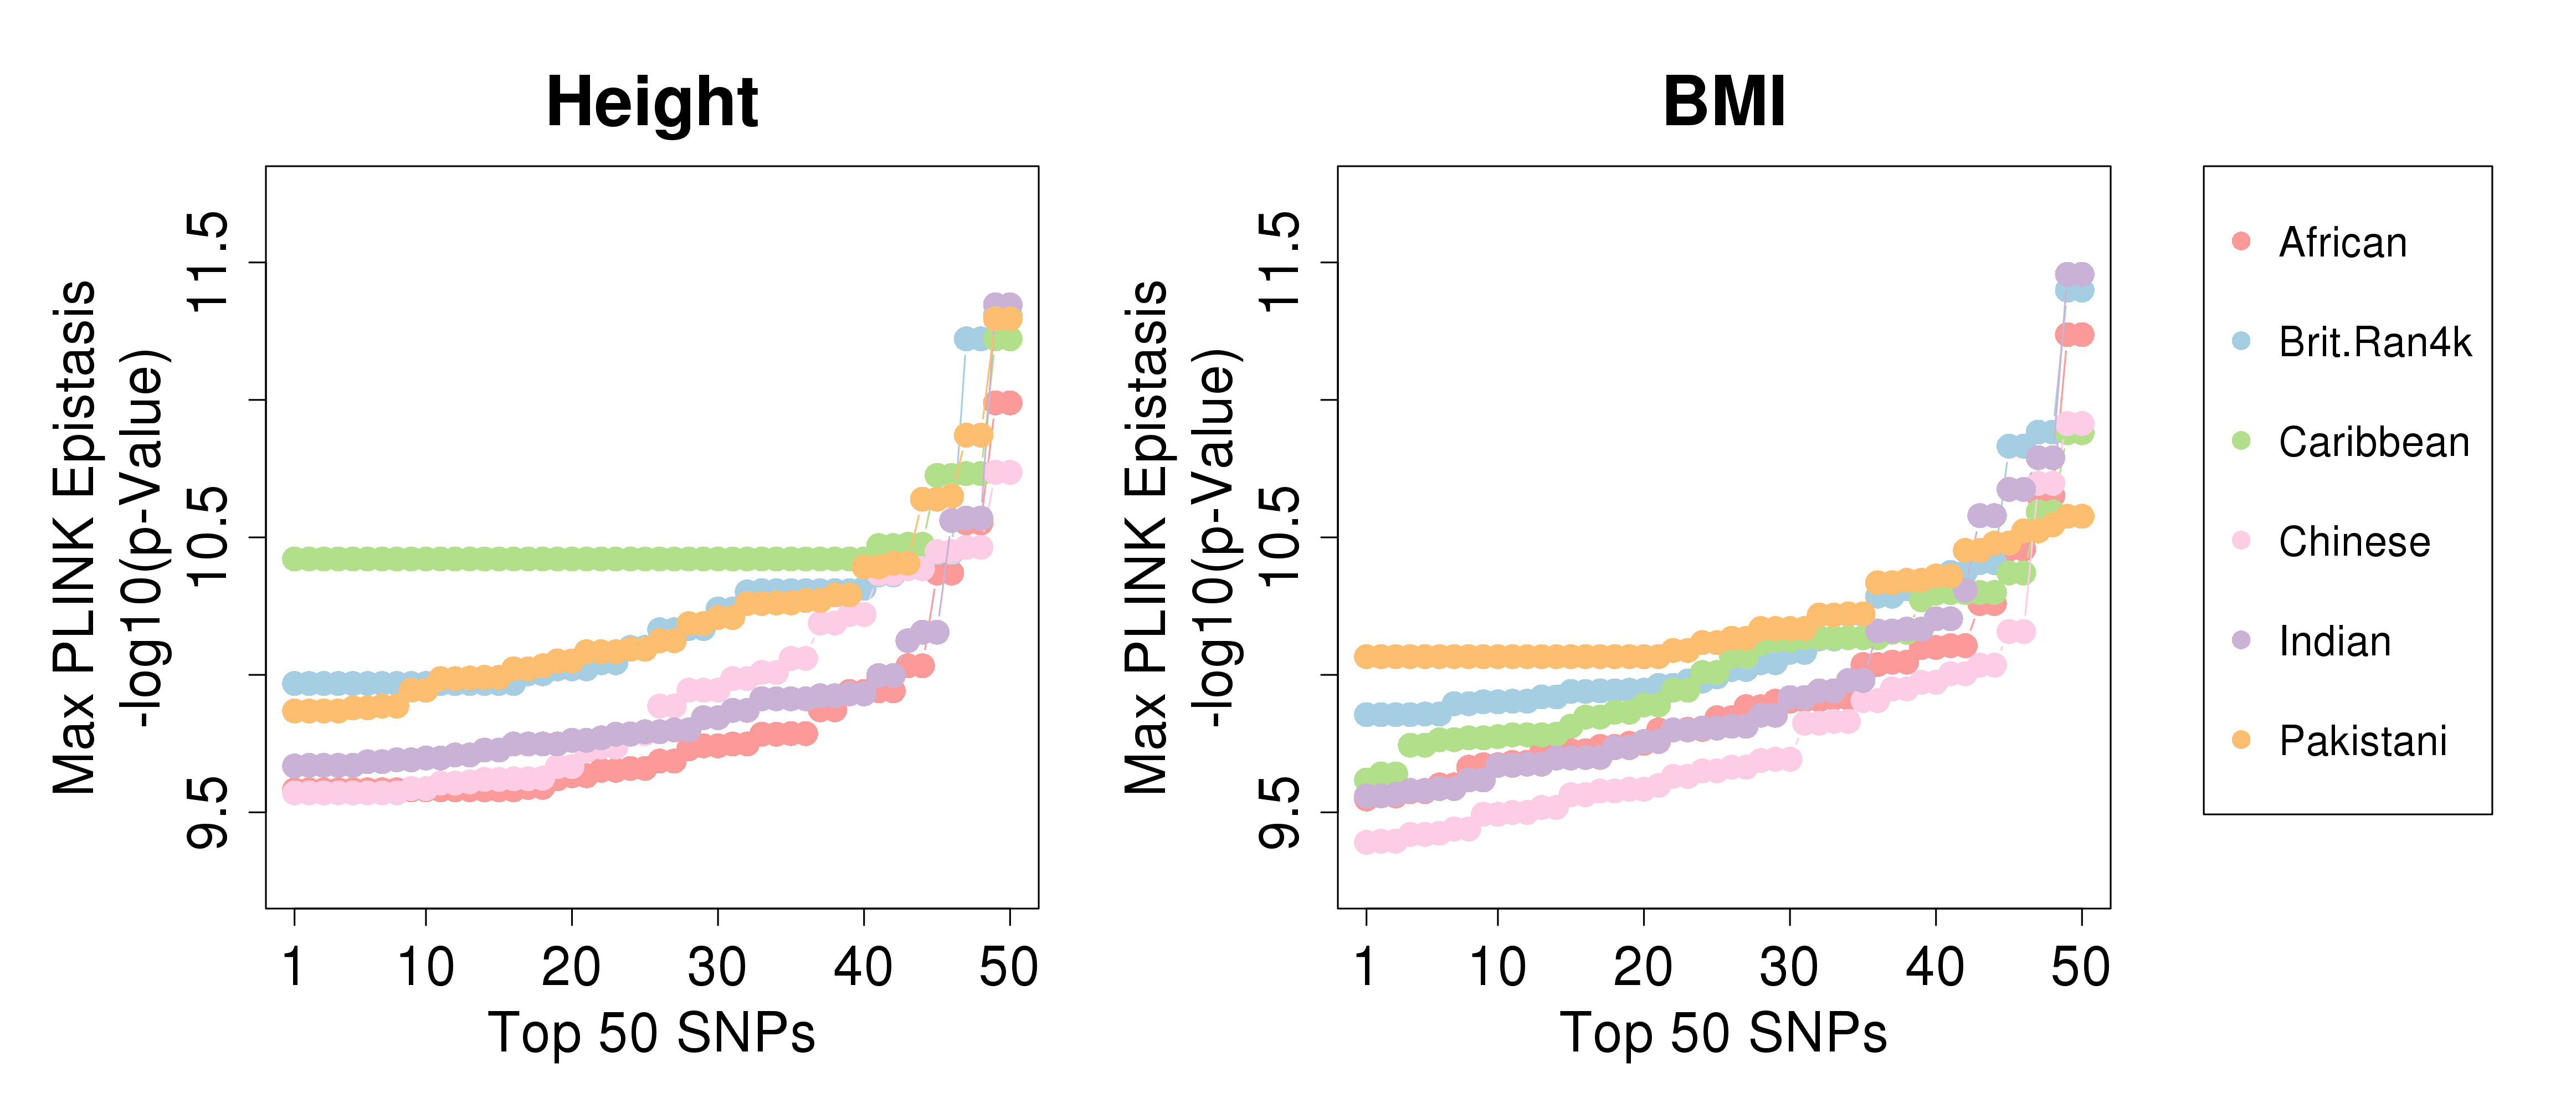
\includegraphics[scale=.45]{Images/Supp/InterPath_Supp_Figure_PLINK_BestSNPs_vs2_AllPops_HeightBMI.png}
%\caption[TBD]{\textbf{SNPs with the largest PLINK pairwise epistasis signals, per subgroup}. The figure shows the best $p$-values obtained from running PLINK's exhaustive pairwise SNP epistasis test for both height and BMI in each of the UKB subgroups. Only the top 50 SNPs, sorted by best pairwise SNP epistasis $p$-value, for each subgroup are shown. No test reaches genome-wide significance based on using a Bonferroni-corrected $p$-value threshold ($p$-value $< 5\times10^{-13}$).}
%\label{InterPath-Supp-Figure-PLINK-HeightBMI-AllPops}
%\end{figure}
%\clearpage

%From: ,https://tex.stackexchange.com/questions/64934/subfig-label-positioning, https://tex.stackexchange.com/questions/196653/how-do-i-stack-two-figures-on-top-of-each-other-rather-than-side-to-side, https://tex.stackexchange.com/questions/47311/include-table-as-a-subfigure, https://tex.stackexchange.com/questions/169541/looking-for-three-images-on-top-of-each-other-with-text-underneath-each, https://tex.stackexchange.com/questions/10863/is-there-a-way-to-slightly-shrink-a-table-including-font-size-to-fit-within-th

\newcounter{CharNumber5}
\setcounter{CharNumber5}{1}
\renewcommand{\thefigure}{\arabic{figure}\alph{CharNumber5}}
\begin{figure}[ht]
\centering
\vspace*{-.5cm}
\subfloat[]{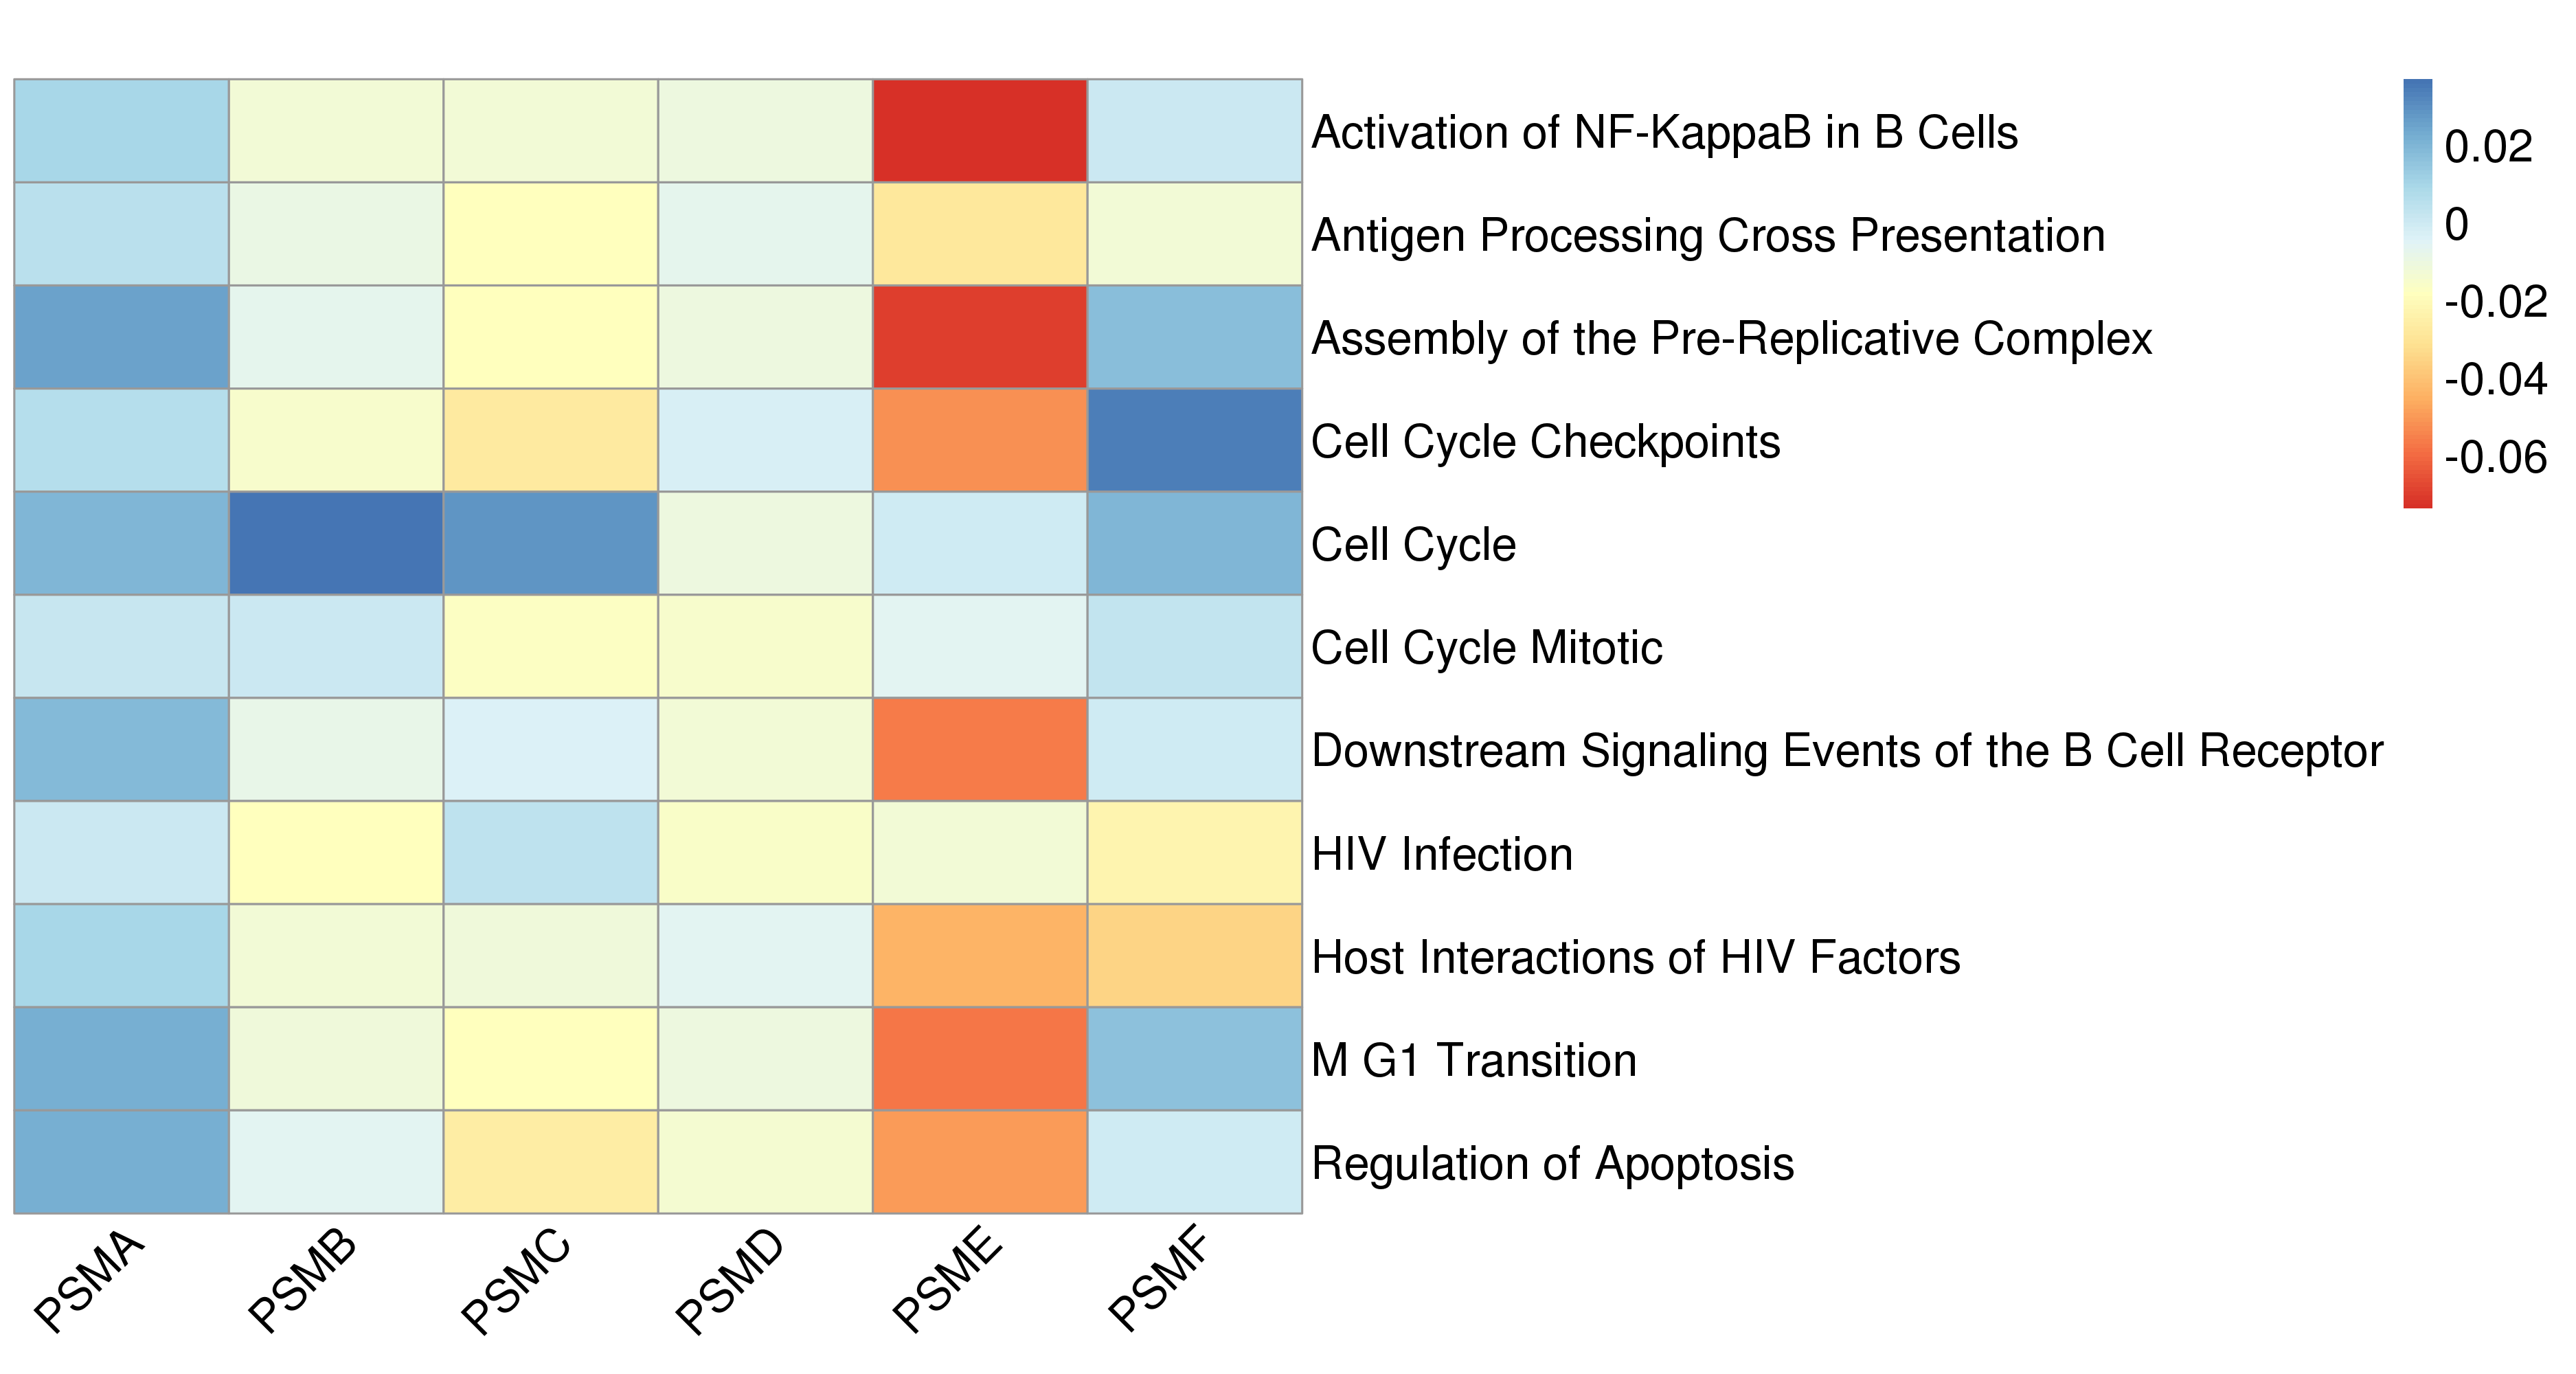
\includegraphics[scale=.5]{Images/Supp/InterPath_Supp_Figure_Proteaseome_Heatplots_African_Loop_vs3.png}}
\par
\subfloat[]{\resizebox{1.1\columnwidth}{!}{
 \hspace*{-1.75cm}
 \begin{tabular}{cc|ccc}
  \hline
\textbf{Proteasome} & \textbf{SNPs} & \textbf{REACTOME} & \textbf{SNPs} & \textbf{MAPIT-R} \\
 \textbf{Gene Family} & & \textbf{Pathway} & & \textbf{$p$-Value} \\
  \hline
PSMA & 17 & Activation of NF-KappaB in B Cells & 465 & 1.86E-05  \\
PSMB & 74 & Antigen Processing Cross Presentation & 850 & 3.96E-05 \\
PSMC & 20 & Assembly of the Pre-Replicative Complex & 331 & 3.29E-05 \\
PSMD & 62 & Cell Cycle Checkpoints & 670 & 5.78E-06 \\
PSME & 15 & Cell Cycle & 2459 & 1.29E-06 \\
PSMF & 16 & Cell Cycle Mitotic & 1906 & 4.51E-05 \\
 & & Downstream Signaling Events of the B Cell Receptor & 745 & 1.19E-05 \\
 & & HIV Infection & 1346 & 7.53E-07 \\
 & & Host Interactions of HIV Factors & 963 & 7.52E-06 \\
 & & M G1 Transition & 458 & 3.19E-06 \\
 & & Regulation of Apoptosis & 564 & 1.22E-05 \\
  \hline
\end{tabular}}}
\caption[TBD]{\textbf{Proteasome gene family leave-one-out MAPIT-R reruns, REACTOME-BMI-African}. (a) The figure shows the change in original MAPIT-R -$\log_{10}$ $p$-value for each presented REACTOME pathway when each proteasome gene family is removed one at a time. The analyses were conducted in the BMI-African subgroup combination. The $x$-axis shows each proteasome gene family and the $y$-axis shows each REACTOME pathway. Each column has been scaled by the number of SNPs present in the given gene family and, as a result, the heatplot specifically shows the -$\log_{10}$ $p$-value change per SNP. (b) The table shows the number of SNPs that are present in each proteasome gene family (left) and each REACTOME pathway (right). The original MAPIT-R $p$-values for each pathway are also shown (right).}
\label{InterPath-Supp-Figure-Prot-Heatplots-African}
\end{figure}
\clearpage
\addtocounter{figure}{-1}
\addtocounter{CharNumber5}{1}

%\captionsetup[subfigure]{position=top, labelfont=bf,textfont=normalfont,singlelinecheck=off,justification=raggedright}

\begin{figure}[ht]
\centering
\vspace*{-.5cm}
\subfloat[]{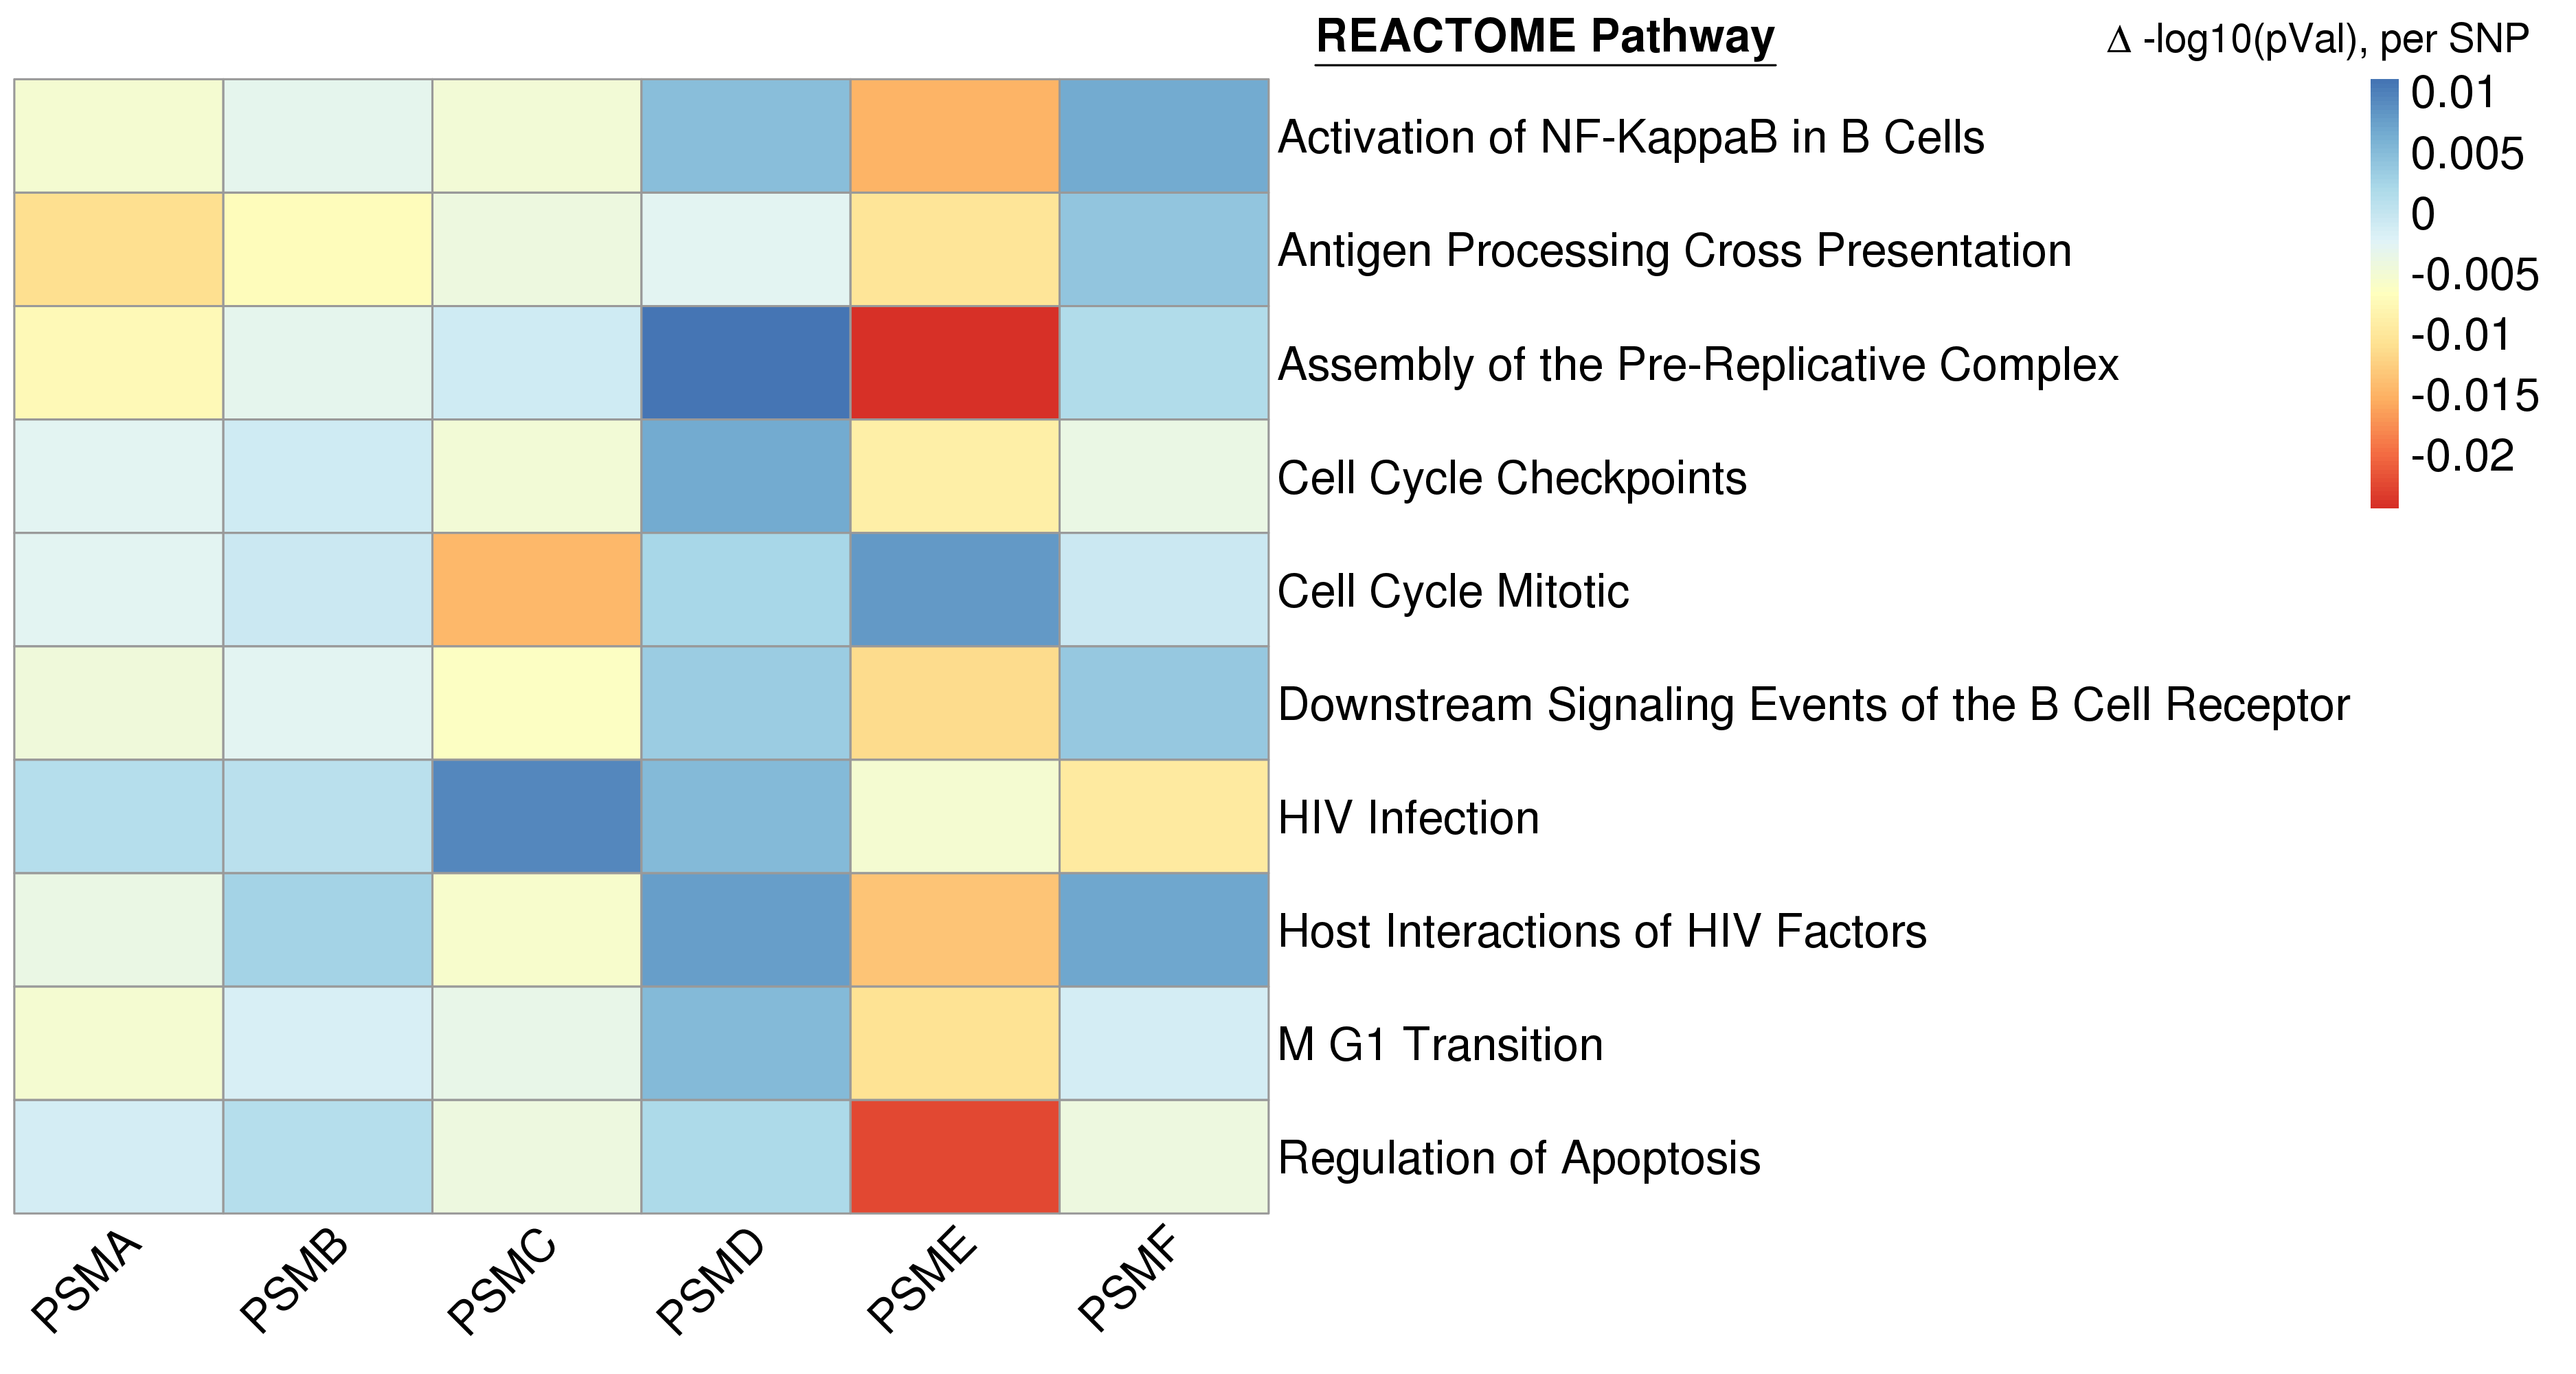
\includegraphics[scale=.5]{Images/Supp/InterPath_Supp_Figure_Proteaseome_Heatplots_BritRan4000_Loop_vs3.png}}
\par
\subfloat[]{\resizebox{1.1\columnwidth}{!}{
 \hspace*{-1.75cm}
 \begin{tabular}{cc|ccc}
  \hline
\textbf{Proteasome} & \textbf{SNPs} & \textbf{REACTOME} & \textbf{SNPs} & \textbf{MAPIT-R} \\
 \textbf{Gene Family} & & \textbf{Pathway} & & \textbf{$p$-Value} \\
  \hline
PSMA & 40 & Activation of NF-KappaB in B Cells & 756 & 2.28E-01  \\
PSMB & 91 & Antigen Processing Cross Presentation & 1104 & 2.48E-05 \\
PSMC & 29 & Assembly of the Pre-Replicative Complex & 507 & 1.84E-02 \\
PSMD & 101 & Cell Cycle Checkpoints & 1121 & 6.77E-02 \\
PSME & 25 & Cell Cycle Mitotic & 3304 & 2.34E-01 \\
 PSMF & 26 & Downstream Signaling Events of the B Cell Receptor & 1248 & 3.25E-01 \\
 & & HIV Infection & 2221 & 8.26E-02 \\
 & & Host Interactions of HIV Factors & 1541 & 1.55E-02 \\
 & & M G1 Transition & 697 & 3.02E-01 \\
 & & Regulation of Apoptosis & 906 & 2.98E-02 \\
  \hline
\end{tabular}}}
\caption[TBD]{\textbf{Proteasome gene family leave-one-out MAPIT-R reruns, REACTOME-BMI-British.Ran4000}. (a) The figure shows the change in original MAPIT-R -$\log_{10}$ $p$-value for each presented REACTOME pathway when each proteasome gene family is removed one at a time. The analyses were conducted in the BMI-British.Ran4000 subgroup combination. The $x$-axis shows each proteasome gene family and the $y$-axis shows each REACTOME pathway. Each column has been scaled by the number of SNPs present in the given gene family and, as a result, the heatplot specifically shows the -$\log_{10}$ $p$-value change per SNP. (b) The table shows the number of SNPs that are present in each proteasome gene family (left) and each REACTOME pathway (right). The original MAPIT-R $p$-values for each pathway are also shown (right).}
\label{InterPath-Supp-Figure-Prot-Heatplots-BritRan4000}
\end{figure}
\clearpage
\addtocounter{figure}{-1}
\addtocounter{CharNumber5}{1}

\begin{figure}[ht]
\centering
\vspace*{-.5cm}
\subfloat[]{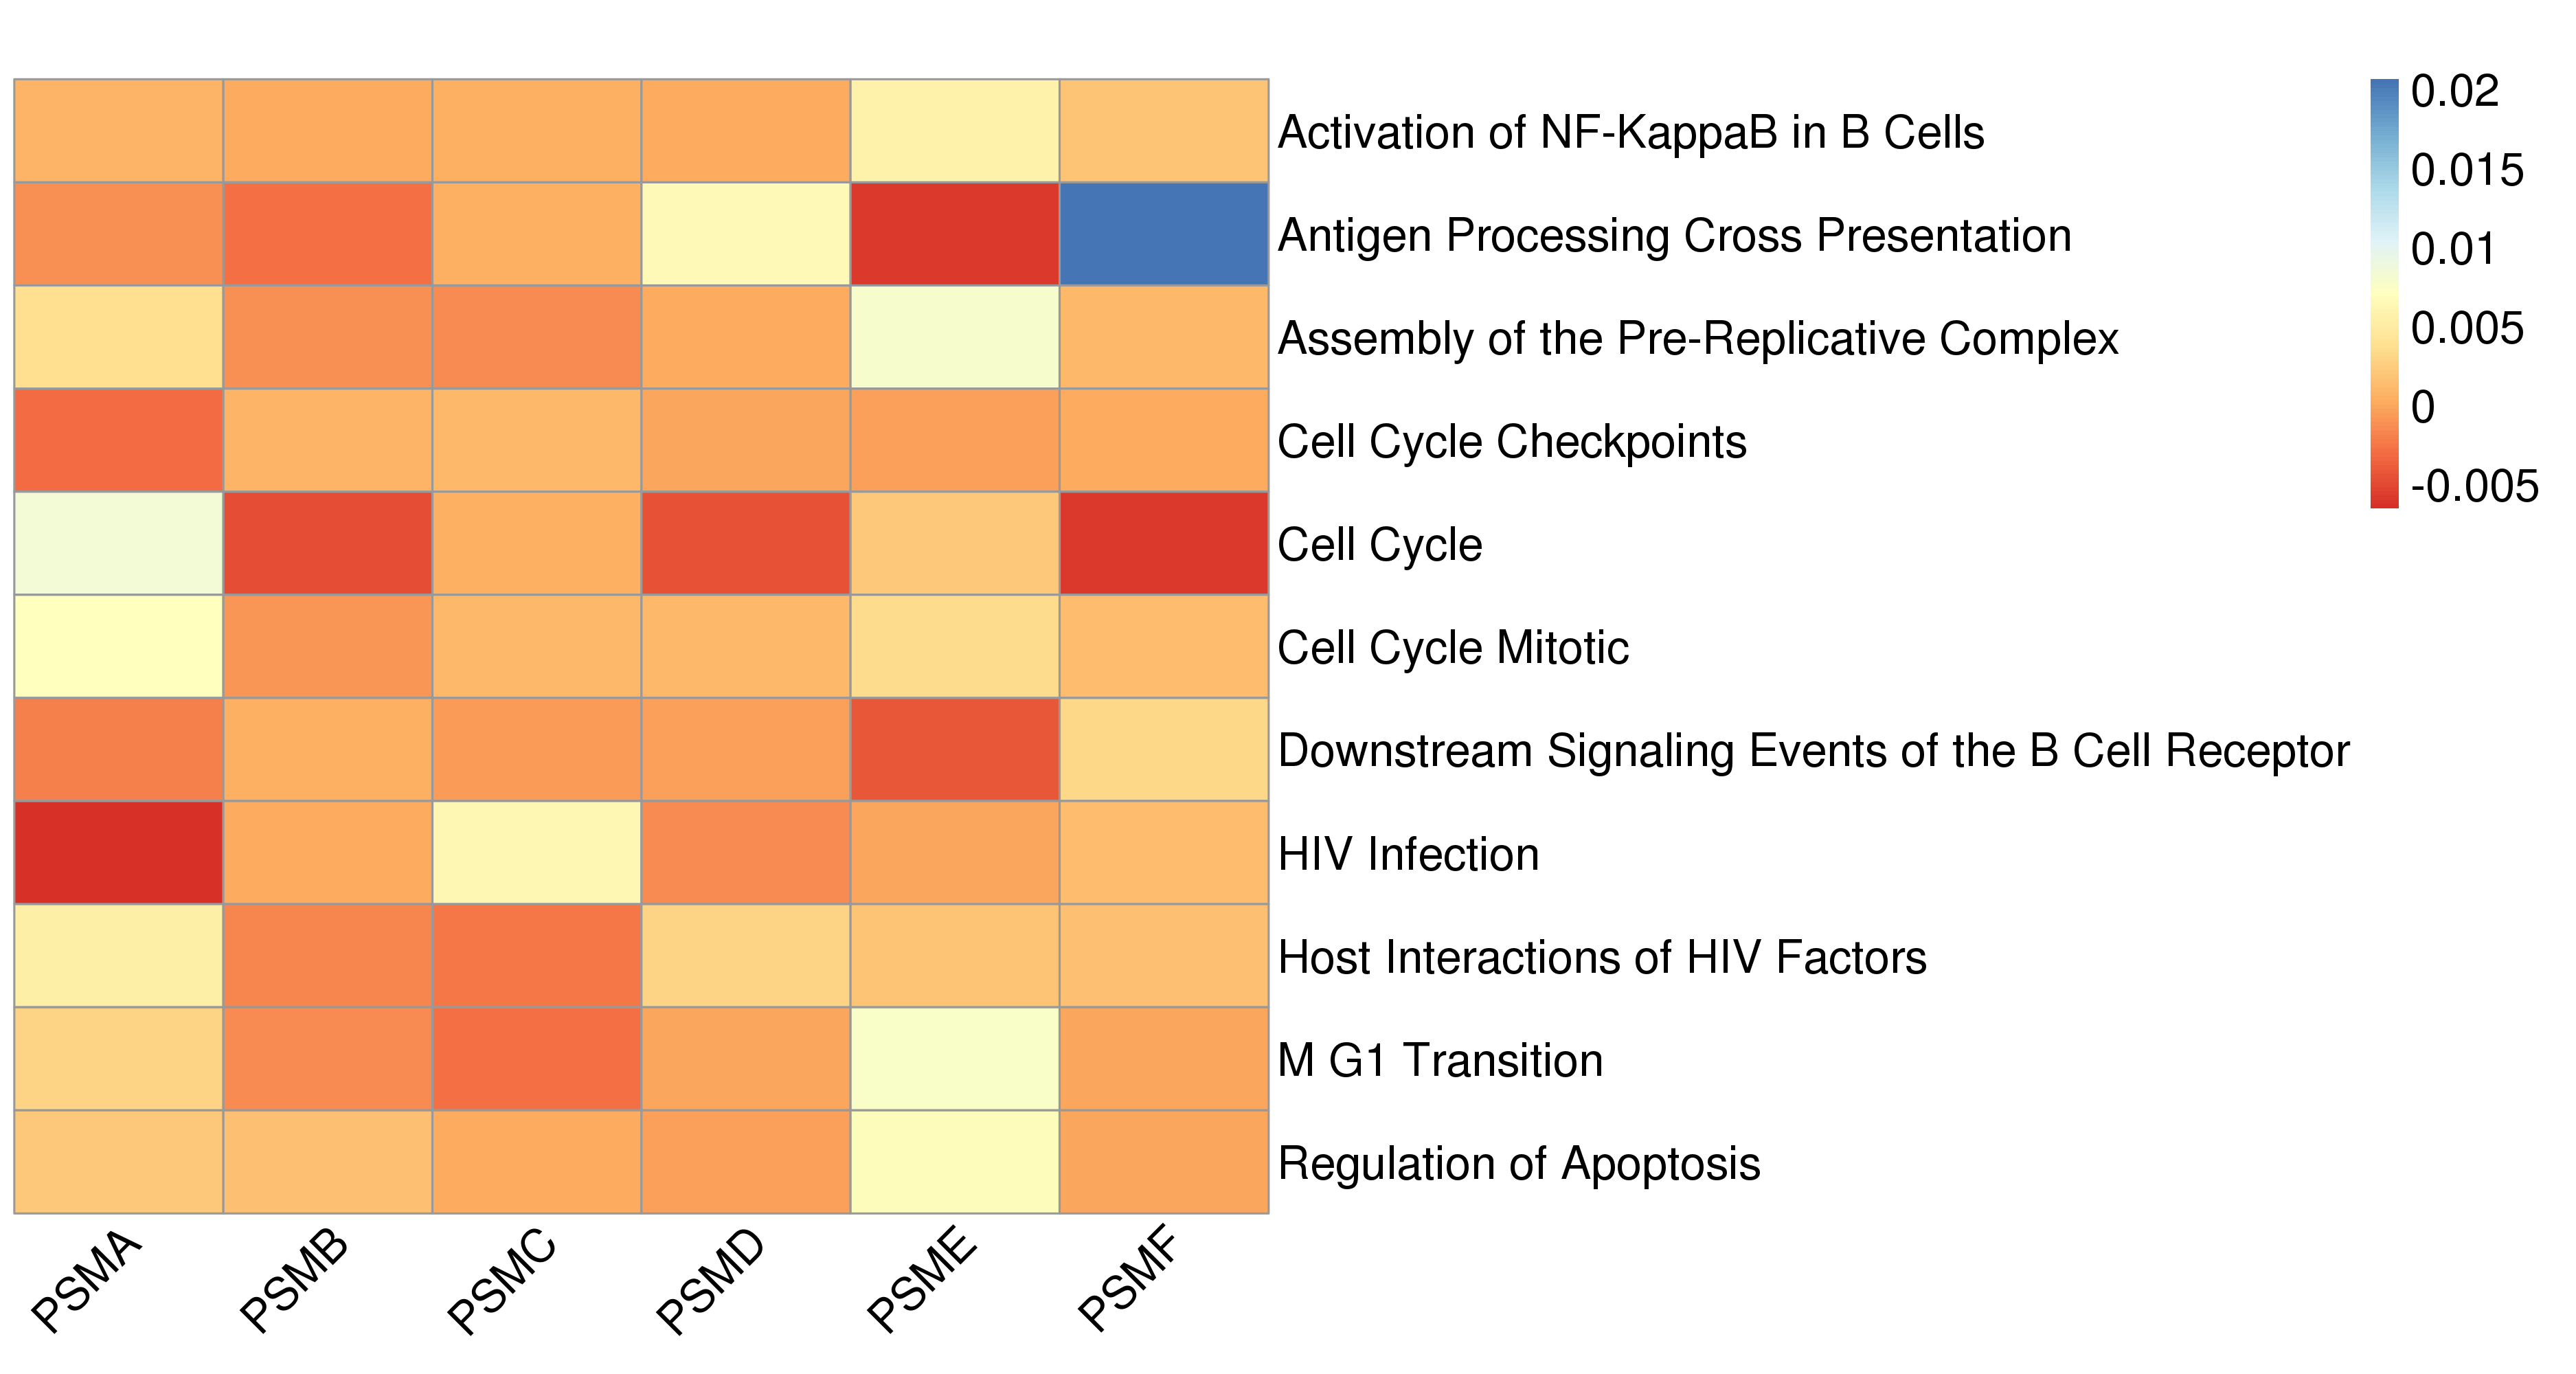
\includegraphics[scale=.5]{Images/Supp/InterPath_Supp_Figure_Proteaseome_Heatplots_Caribbean_Loop_vs3.png}}
\par
\subfloat[]{\resizebox{1.1\columnwidth}{!}{
 \hspace*{-1.75cm}
 \begin{tabular}{cc|ccc}
  \hline
\textbf{Proteasome} & \textbf{SNPs} & \textbf{REACTOME} & \textbf{SNPs} & \textbf{MAPIT-R} \\
 \textbf{Gene Family} & & \textbf{Pathway} & & \textbf{$p$-Value} \\
  \hline
PSMA & 18 & Activation of NF-KappaB in B Cells & 507 & 9.93E-01  \\
PSMB & 77 & Antigen Processing Cross Presentation & 871 & 5.15E-02 \\
PSMC & 21 & Assembly of the Pre-Replicative Complex & 357 & 7.25E-01 \\
PSMD & 69 & Cell Cycle Checkpoints & 736 & 8.83E-01 \\
PSME & 15 & Cell Cycle & 2711 & 2.51E-01 \\
PSMF & 16 & Cell Cycle Mitotic & 2111 & 7.98E-01 \\
 & & Downstream Signaling Events of the B Cell Receptor & 829 & 8.37E-01 \\
 & & HIV Infection & 1483 & 3.11E-01 \\
 & & Host Interactions of HIV Factors & 1055 & 6.68E-01 \\
 & & M G1 Transition & 500 & 6.37E-01 \\
 & & Regulation of Apoptosis & 615 & 9.42E-01 \\
  \hline
\end{tabular}}}
\caption[TBD]{\textbf{Proteasome gene family leave-one-out MAPIT-R reruns, REACTOME-BMI-Caribbean}. (a) The figure shows the change in original MAPIT-R -$\log_{10}$ $p$-value for each presented REACTOME pathway when each proteasome gene family is removed one at a time. The analyses were conducted in the BMI-Caribbean subgroup combination. The $x$-axis shows each proteasome gene family and the $y$-axis shows each REACTOME pathway. Each column has been scaled by the number of SNPs present in the given gene family and, as a result, the heatplot specifically shows the -$\log_{10}$ $p$-value change per SNP. (b) The table shows the number of SNPs that are present in each proteasome gene family (left) and each REACTOME pathway (right). The original MAPIT-R $p$-values for each pathway are also shown (right).}
\label{InterPath-Supp-Figure-Prot-Heatplots-Caribbean}
\end{figure}
\clearpage
\addtocounter{figure}{-1}
\addtocounter{CharNumber5}{1}

\begin{figure}[ht]
\centering
\vspace*{-.5cm}
\subfloat[]{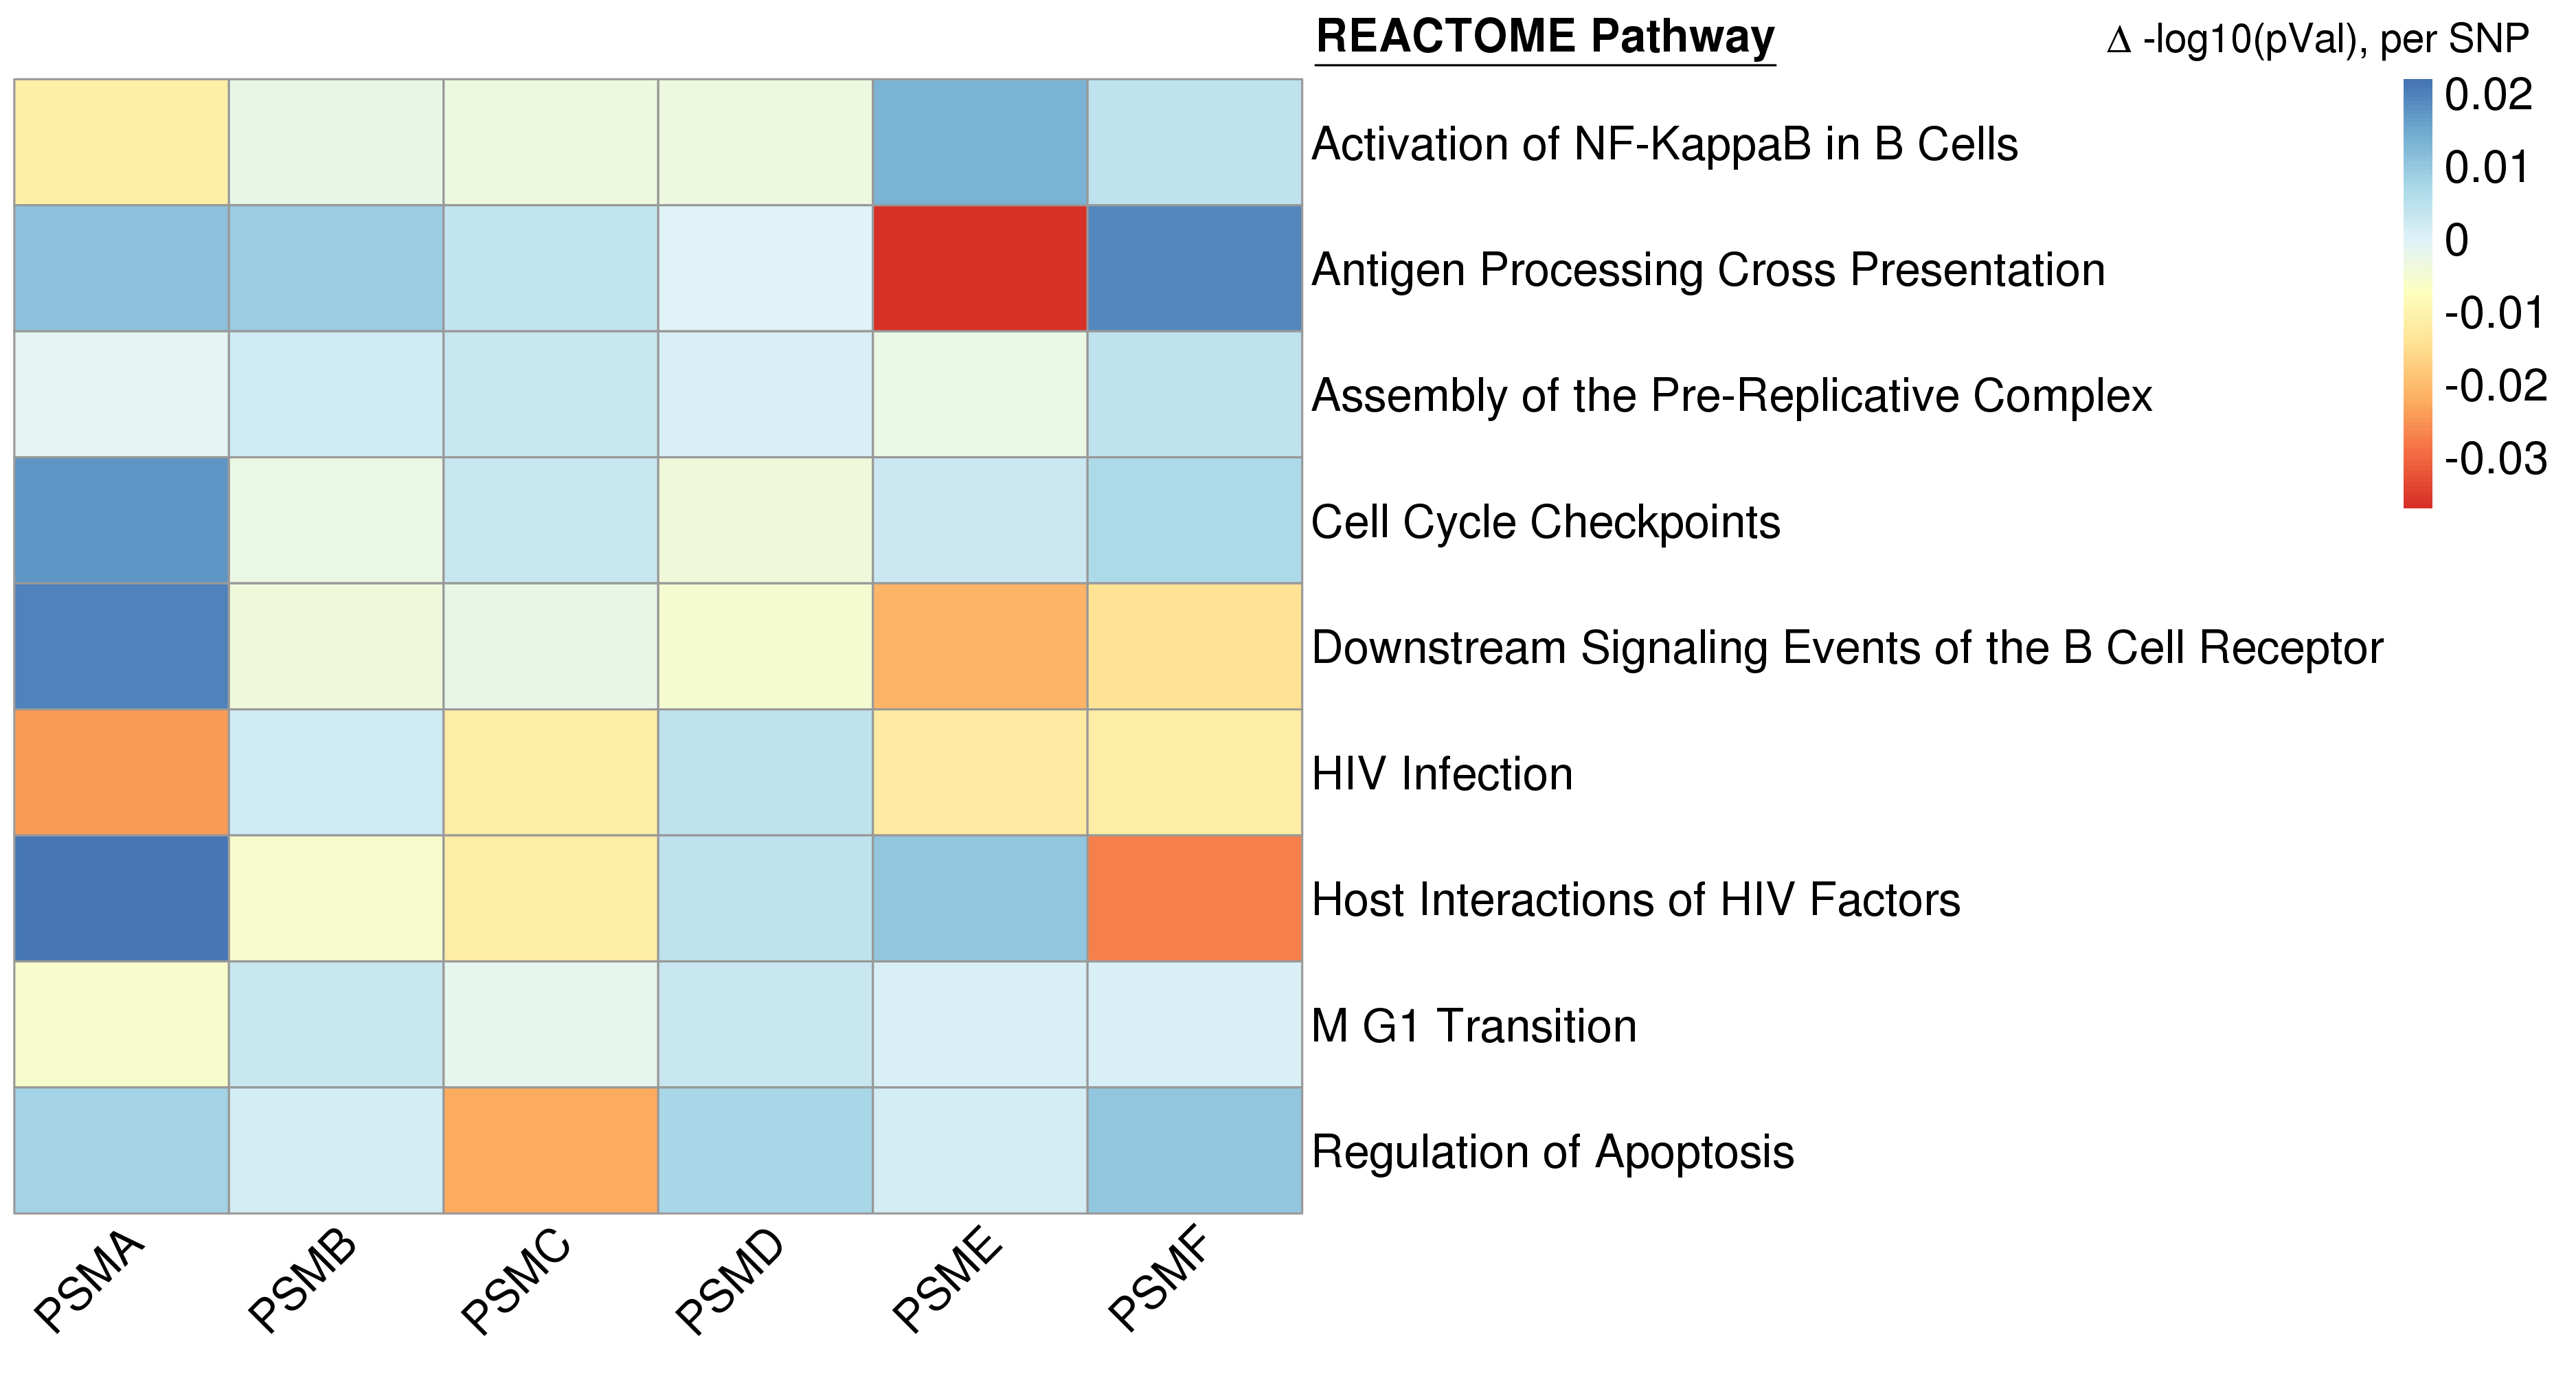
\includegraphics[scale=.5]{Images/Supp/InterPath_Supp_Figure_Proteaseome_Heatplots_Chinese_Loop_vs3.png}}
\par
\subfloat[]{\resizebox{1.1\columnwidth}{!}{
 \hspace*{-1.75cm}
 \begin{tabular}{cc|ccc}
  \hline
\textbf{Proteasome} & \textbf{SNPs} & \textbf{REACTOME} & \textbf{SNPs} & \textbf{MAPIT-R} \\
 \textbf{Gene Family} & & \textbf{Pathway} & & \textbf{$p$-Value} \\
  \hline
PSMA & 13 & Activation of NF-KappaB in B Cells & 433 & 5.27E-01  \\
PSMB & 74 & Antigen Processing Cross Presentation & 771 & 1.11E-02 \\
PSMC & 18 & Assembly of the Pre-Replicative Complex & 292 & 8.77E-01 \\
PSMD & 58 & Cell Cycle Checkpoints & 589 & 5.41E-01  \\
PSME & 12 & Downstream Signaling Events of the B Cell Receptor & 698 & 1.40E-01 \\
PSMF & 16 & HIV Infection & 1266 & 3.68E-03 \\
 & & Host Interactions of HIV Factors & 902 & 4.24E-02 \\
 & & M G1 Transition & 400 & 8.20E-01 \\
 & & Regulation of Apoptosis & 527 & 2.26E-02 \\
  \hline
\end{tabular}}}
\caption[TBD]{\textbf{Proteasome gene family leave-one-out MAPIT-R reruns, REACTOME-BMI-Chinese}. (a) The figure shows the change in original MAPIT-R -$\log_{10}$ $p$-value for each presented REACTOME pathway when each proteasome gene family is removed one at a time. The analyses were conducted in the BMI-Chinese subgroup combination. The $x$-axis shows each proteasome gene family and the $y$-axis shows each REACTOME pathway. Each column has been scaled by the number of SNPs present in the given gene family and, as a result, the heatplot specifically shows the -$\log_{10}$ $p$-value change per SNP. (b) The table shows the number of SNPs that are present in each proteasome gene family (left) and each REACTOME pathway (right). The original MAPIT-R $p$-values for each pathway are also shown (right).}
\label{InterPath-Supp-Figure-Prot-Heatplots-Chinese}
\end{figure}
\clearpage
\addtocounter{figure}{-1}
\addtocounter{CharNumber5}{1}

\begin{figure}[ht]
\centering
\vspace*{-.5cm}
\subfloat[]{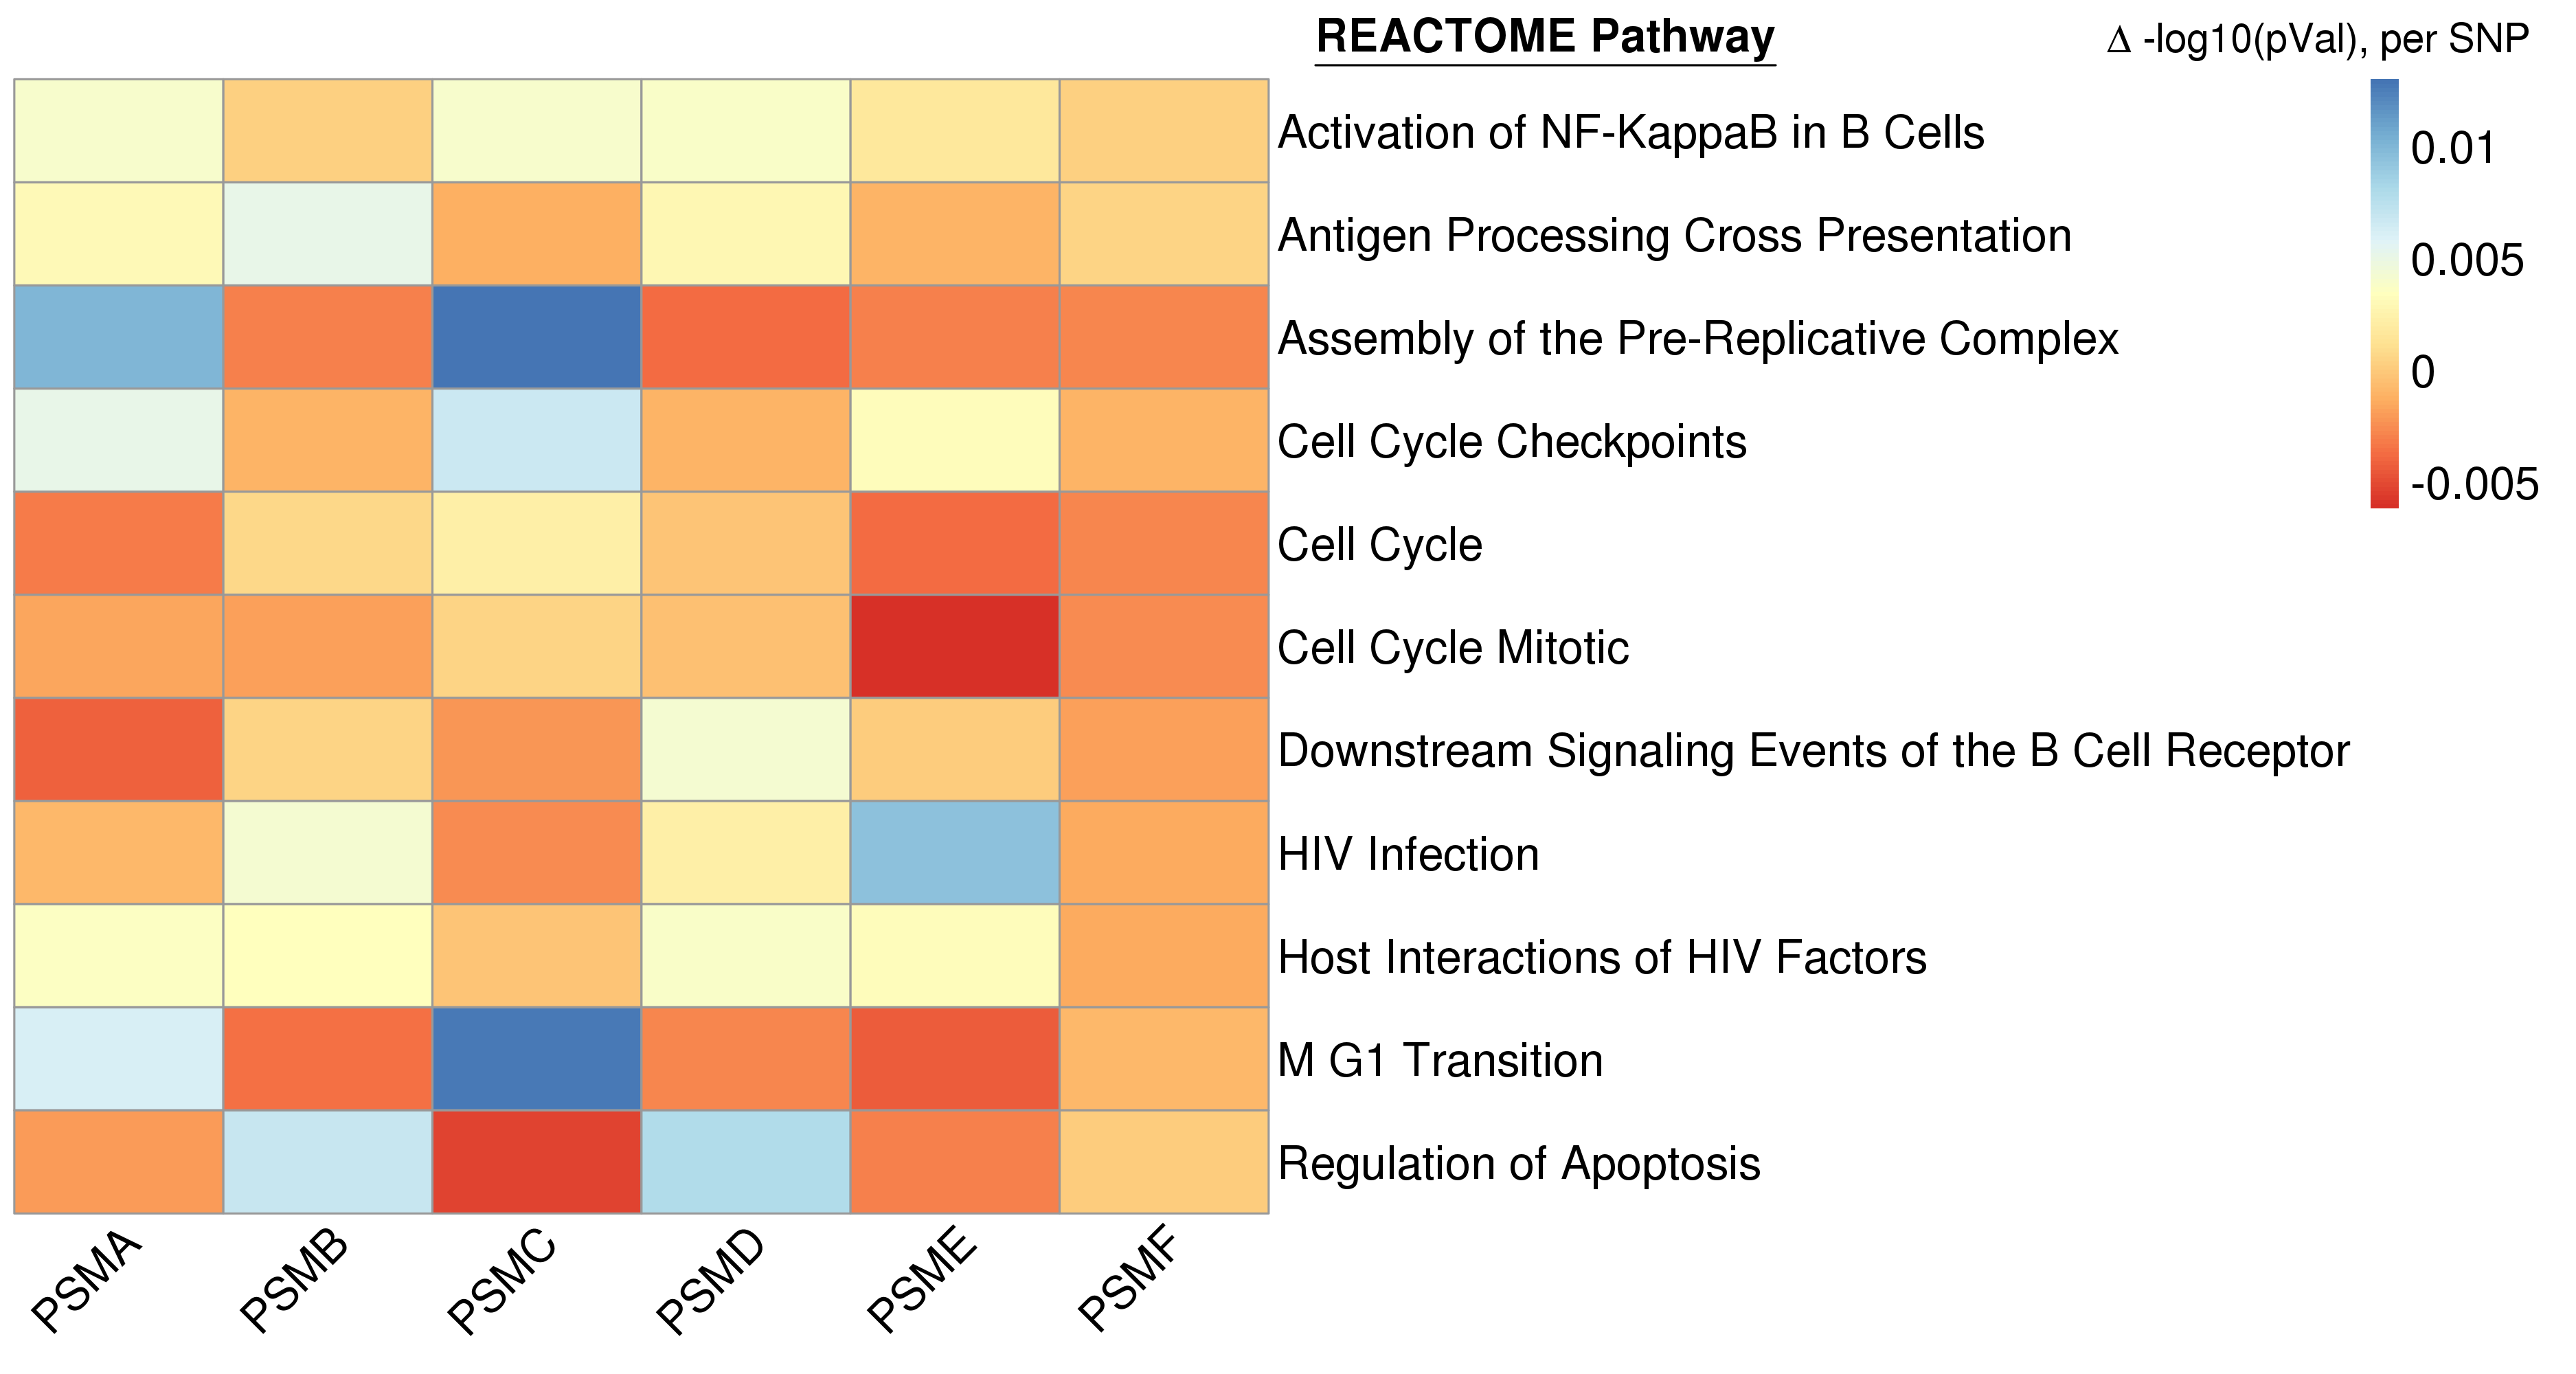
\includegraphics[scale=.5]{Images/Supp/InterPath_Supp_Figure_Proteaseome_Heatplots_Indian_Loop_vs3.png}}
\par
\subfloat[]{\resizebox{1.1\columnwidth}{!}{
 \hspace*{-1.75cm}
 \begin{tabular}{cc|ccc}
  \hline
\textbf{Proteasome} & \textbf{SNPs} & \textbf{REACTOME} & \textbf{SNPs} & \textbf{MAPIT-R} \\
 \textbf{Gene Family} & & \textbf{Pathway} & & \textbf{$p$-Value} \\
  \hline
PSMA & 29 & Activation of NF-KappaB in B Cells & 618 & 9.978E-01  \\
PSMB & 85 & Antigen Processing Cross Presentation & 977 & 4.476E-01 \\
PSMC & 25 & Assembly of the Pre-Replicative Complex & 427 & 5.019E-01 \\
PSMD & 78 & Cell Cycle Checkpoints & 909 & 8.042E-01 \\
PSME & 21 & Cell Cycle & 3361 & 1.873E-01 \\
PSMF & 21 & Cell Cycle Mitotic & 2656 & 2.316E-01 \\
 & & Downstream Signaling Events of the B Cell Receptor & 1037 & 5.534E-01 \\
 & & HIV Infection & 1836 & 9.803E-02 \\
 & & Host Interactions of HIV Factors & 1278 & 3.788E-01 \\
 & & M G1 Transition & 590 & 4.658E-01 \\
 & & Regulation of Apoptosis & 754 & 5.606E-01 \\
  \hline
\end{tabular}}}
\caption[TBD]{\textbf{Proteasome gene family leave-one-out MAPIT-R reruns, REACTOME-BMI-Indian}. (a) The figure shows the change in original MAPIT-R -$\log_{10}$ $p$-value for each presented REACTOME pathway when each proteasome gene family is removed one at a time. The analyses were conducted in the BMI-Indian subgroup combination. The $x$-axis shows each proteasome gene family and the $y$-axis shows each REACTOME pathway. Each column has been scaled by the number of SNPs present in the given gene family and, as a result, the heatplot specifically shows the -$\log_{10}$ $p$-value change per SNP. (b) The table shows the number of SNPs that are present in each proteasome gene family (left) and each REACTOME pathway (right). The original MAPIT-R $p$-values for each pathway are also shown (right).}
\label{InterPath-Supp-Figure-Prot-Heatplots-Indian}
\end{figure}
\clearpage
\addtocounter{figure}{-1}
\addtocounter{CharNumber5}{1}

\begin{figure}[ht]
\centering
\vspace*{-.5cm}
\subfloat[]{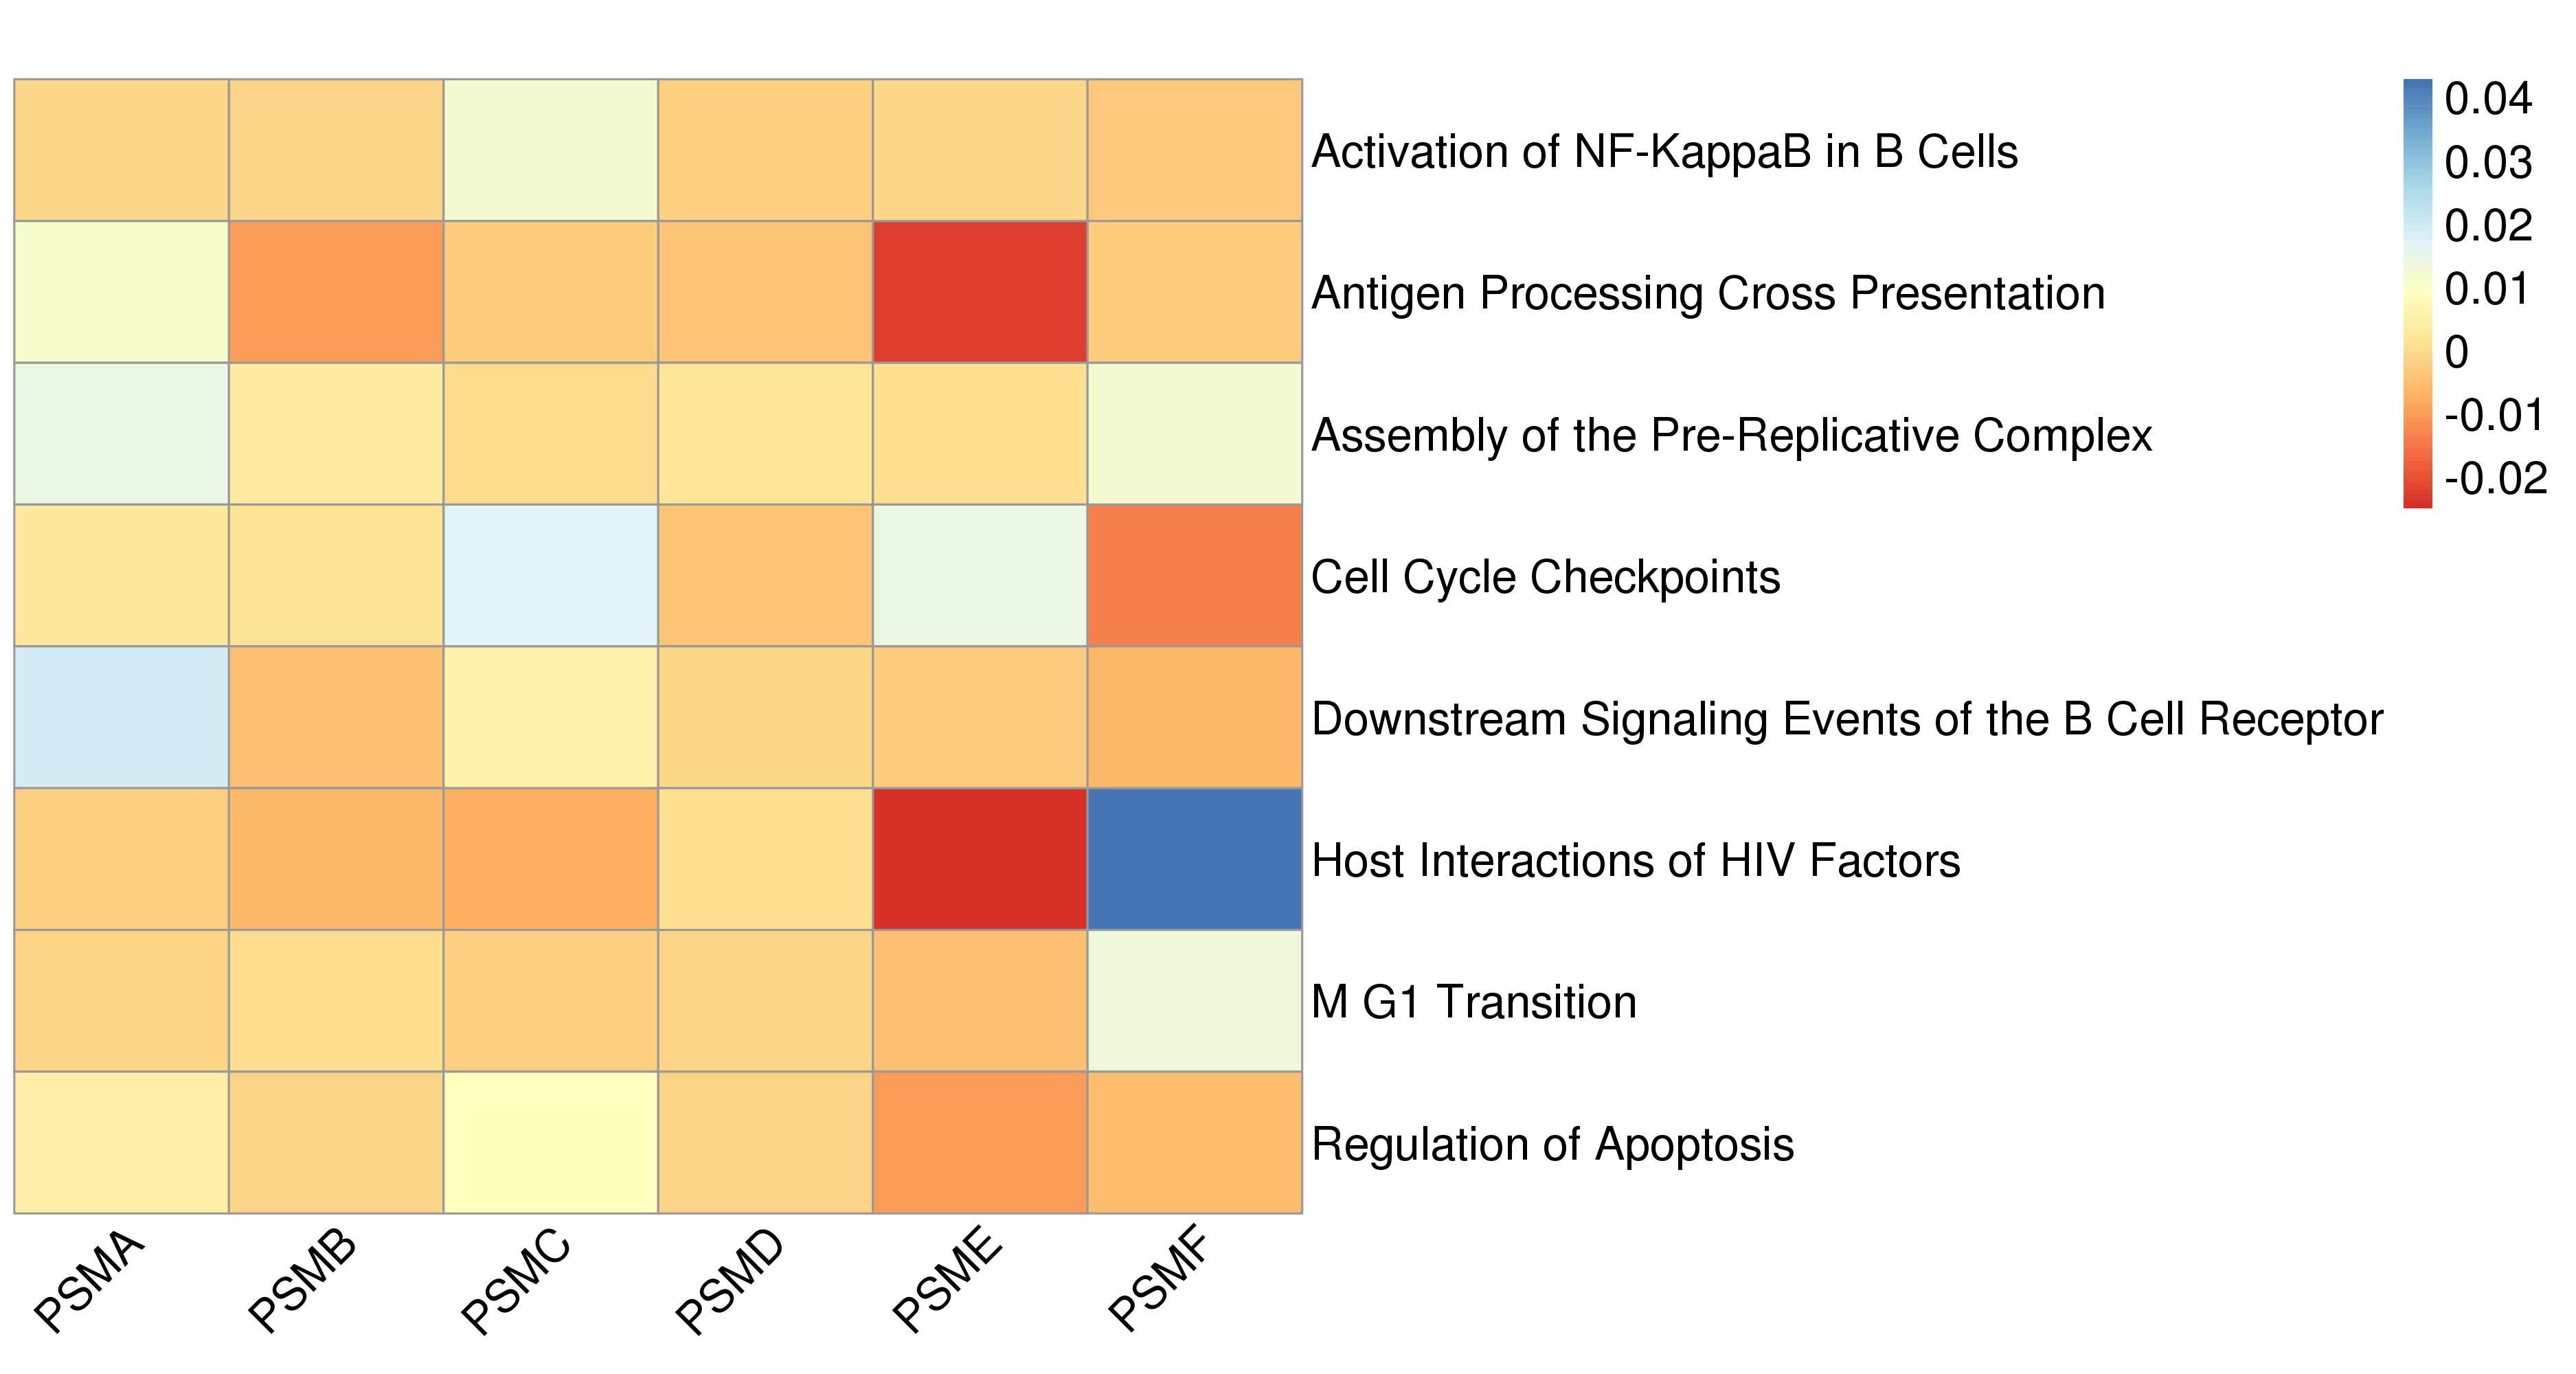
\includegraphics[scale=.5]{Images/Supp/InterPath_Supp_Figure_Proteaseome_Heatplots_Pakistani_Loop_vs3.png}}
\par
\subfloat[]{\resizebox{1.1\columnwidth}{!}{
 \hspace*{-1.75cm}
 \begin{tabular}{cc|ccc}
  \hline
\textbf{Proteasome} & \textbf{SNPs} & \textbf{REACTOME} & \textbf{SNPs} & \textbf{MAPIT-R} \\
 \textbf{Gene Family} & & \textbf{Pathway} & & \textbf{$p$-Value} \\
  \hline
PSMA & 30 & Activation of NF-KappaB in B Cells & 643 & 4.61E-01  \\
PSMB & 90 & Antigen Processing Cross Presentation & 1036 & 8.74E-03 \\
PSMC & 24 & Assembly of the Pre-Replicative Complex & 444 & 9.73E-01 \\
PSMD & 86 & Cell Cycle Checkpoints & 940 & 1.63E-01 \\
PSME & 21 & Downstream Signaling Events of the B Cell Receptor & 1073 & 6.57E-02 \\
PSMF & 22 & Host Interactions of HIV Factors & 1315 & 1.00E-01 \\
 & & M G1 Transition & 612 & 6.66E-01 \\
 & & Regulation of Apoptosis & 774 & 5.16E-02 \\
  \hline
\end{tabular}}}
\caption[TBD]{\textbf{Proteasome gene family leave-one-out MAPIT-R reruns, REACTOME-BMI-Pakistani}. (a) The figure shows the change in original MAPIT-R -$\log_{10}$ $p$-value for each presented REACTOME pathway when each proteasome gene family is removed one at a time. The analyses were conducted in the BMI-Pakistani subgroup combination. The $x$-axis shows each proteasome gene family and the $y$-axis shows each REACTOME pathway. Each column has been scaled by the number of SNPs present in the given gene family and, as a result, the heatplot specifically shows the -$\log_{10}$ $p$-value change per SNP. (b) The table shows the number of SNPs that are present in each proteasome gene family (left) and each REACTOME pathway (right). The original MAPIT-R $p$-values for each pathway are also shown (right).}
\label{InterPath-Supp-Figure-Prot-Heatplots-Pakistani}
\end{figure}
\clearpage
\addtocounter{figure}{-1}
\addtocounter{CharNumber5}{1}

\addtocounter{figure}{1}
\renewcommand{\thefigure}{\arabic{figure}}

\setlength{\footskip}{3cm}
\begin{figure}[htbp]
\centering
\vspace*{-2cm}
\includegraphics[scale=.2]{Images/Supp/InterPath_Supp_Figure_IBS_AllPops_vs4_noHLA.png}
\caption[TBD]{\textbf{Pathway-level genetic diversity vs. MAPIT-R results for all database-phenotype-subgroup combinations}. Caption continued on next page.}
\label{InterPath-Supp-Figure-IBS-AllPops}
\end{figure}
\clearpage
\setlength{\footskip}{1cm}
\addtocounter{figure}{-1}

\begin{figure} [t!]
\caption[TBD]{\textbf{Pathway-level genetic diversity vs. MAPIT-R results for all database-phenotype-subgroup combinations}. The figure shows the mean pairwise IBS proportions per pathway plotted against each pathway's MAPIT-R $p$-value for every pathway database-phenotype-UKB subgroup combination. IBS proportions were calculated per pathway by using that pathway's set of SNPs, were calculated pairwise between every set of individuals in the subgroup, and then averaged across each of these pairs for a final, single summary metric. We observe across the majority of combinations no significant relationship between mean pairwise IBS proportion and MAPIT-R $p$-value.}
\label{InterPath-Supp-Figure-IBS-AllPops-Caption}
\end{figure}
\clearpage

%\begin{figure}[htbp]
%\centering
%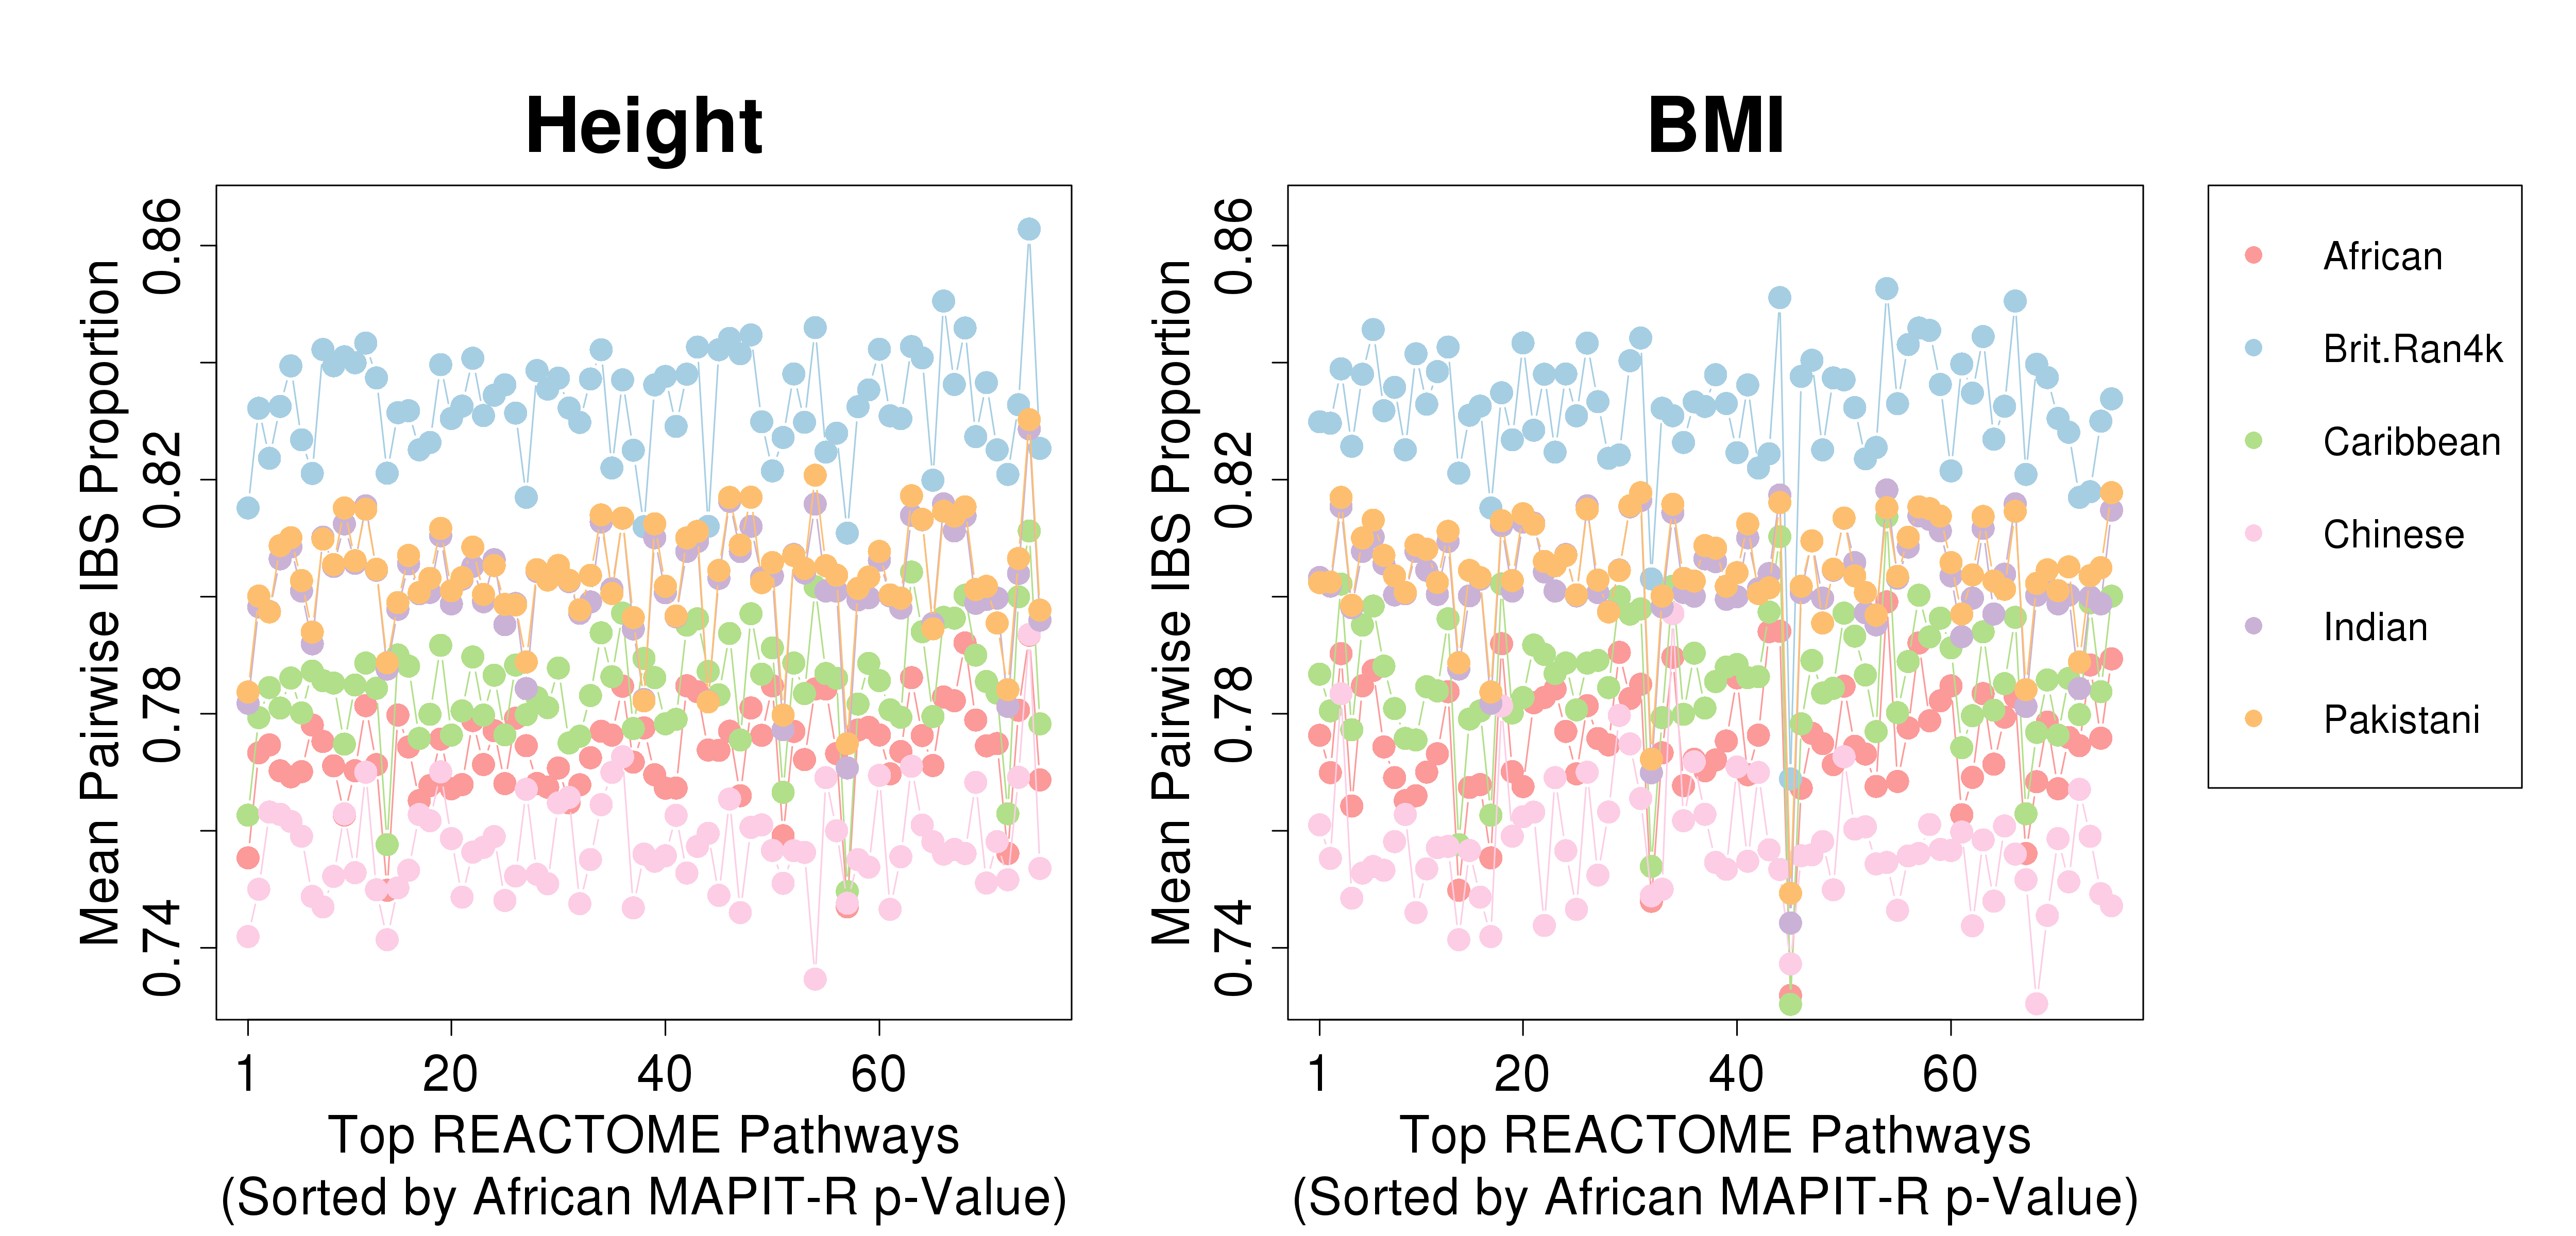
\includegraphics[scale=.35]{Images/Supp/InterPath_Supp_Figure_IBS_AllPopComps_vs3_REACTOME.png}
%\caption[TBD]{\textbf{Pathway-level genetic diversity across all UKB subgroups for top African MAPIT-R REACTOME pathways}. The figure plots the mean pairwise IBS proportions of each UKB subgroup for the top 75 REACTOME pathways (sorted by MAPIT-R African subgroup $p$-value) for each pathway database-phenotype combination. Most variation in mean pairwise IBS proportions varies moreso based on the pathways themselves and not on ancestry; subgroups differ between one another mostly at the same levels across each pathway.}
%\label{InterPath-Supp-Figure-IBS-AllPopComps-REACTOME}
%\end{figure}
%\clearpage

\begin{figure}[htbp]
\centering
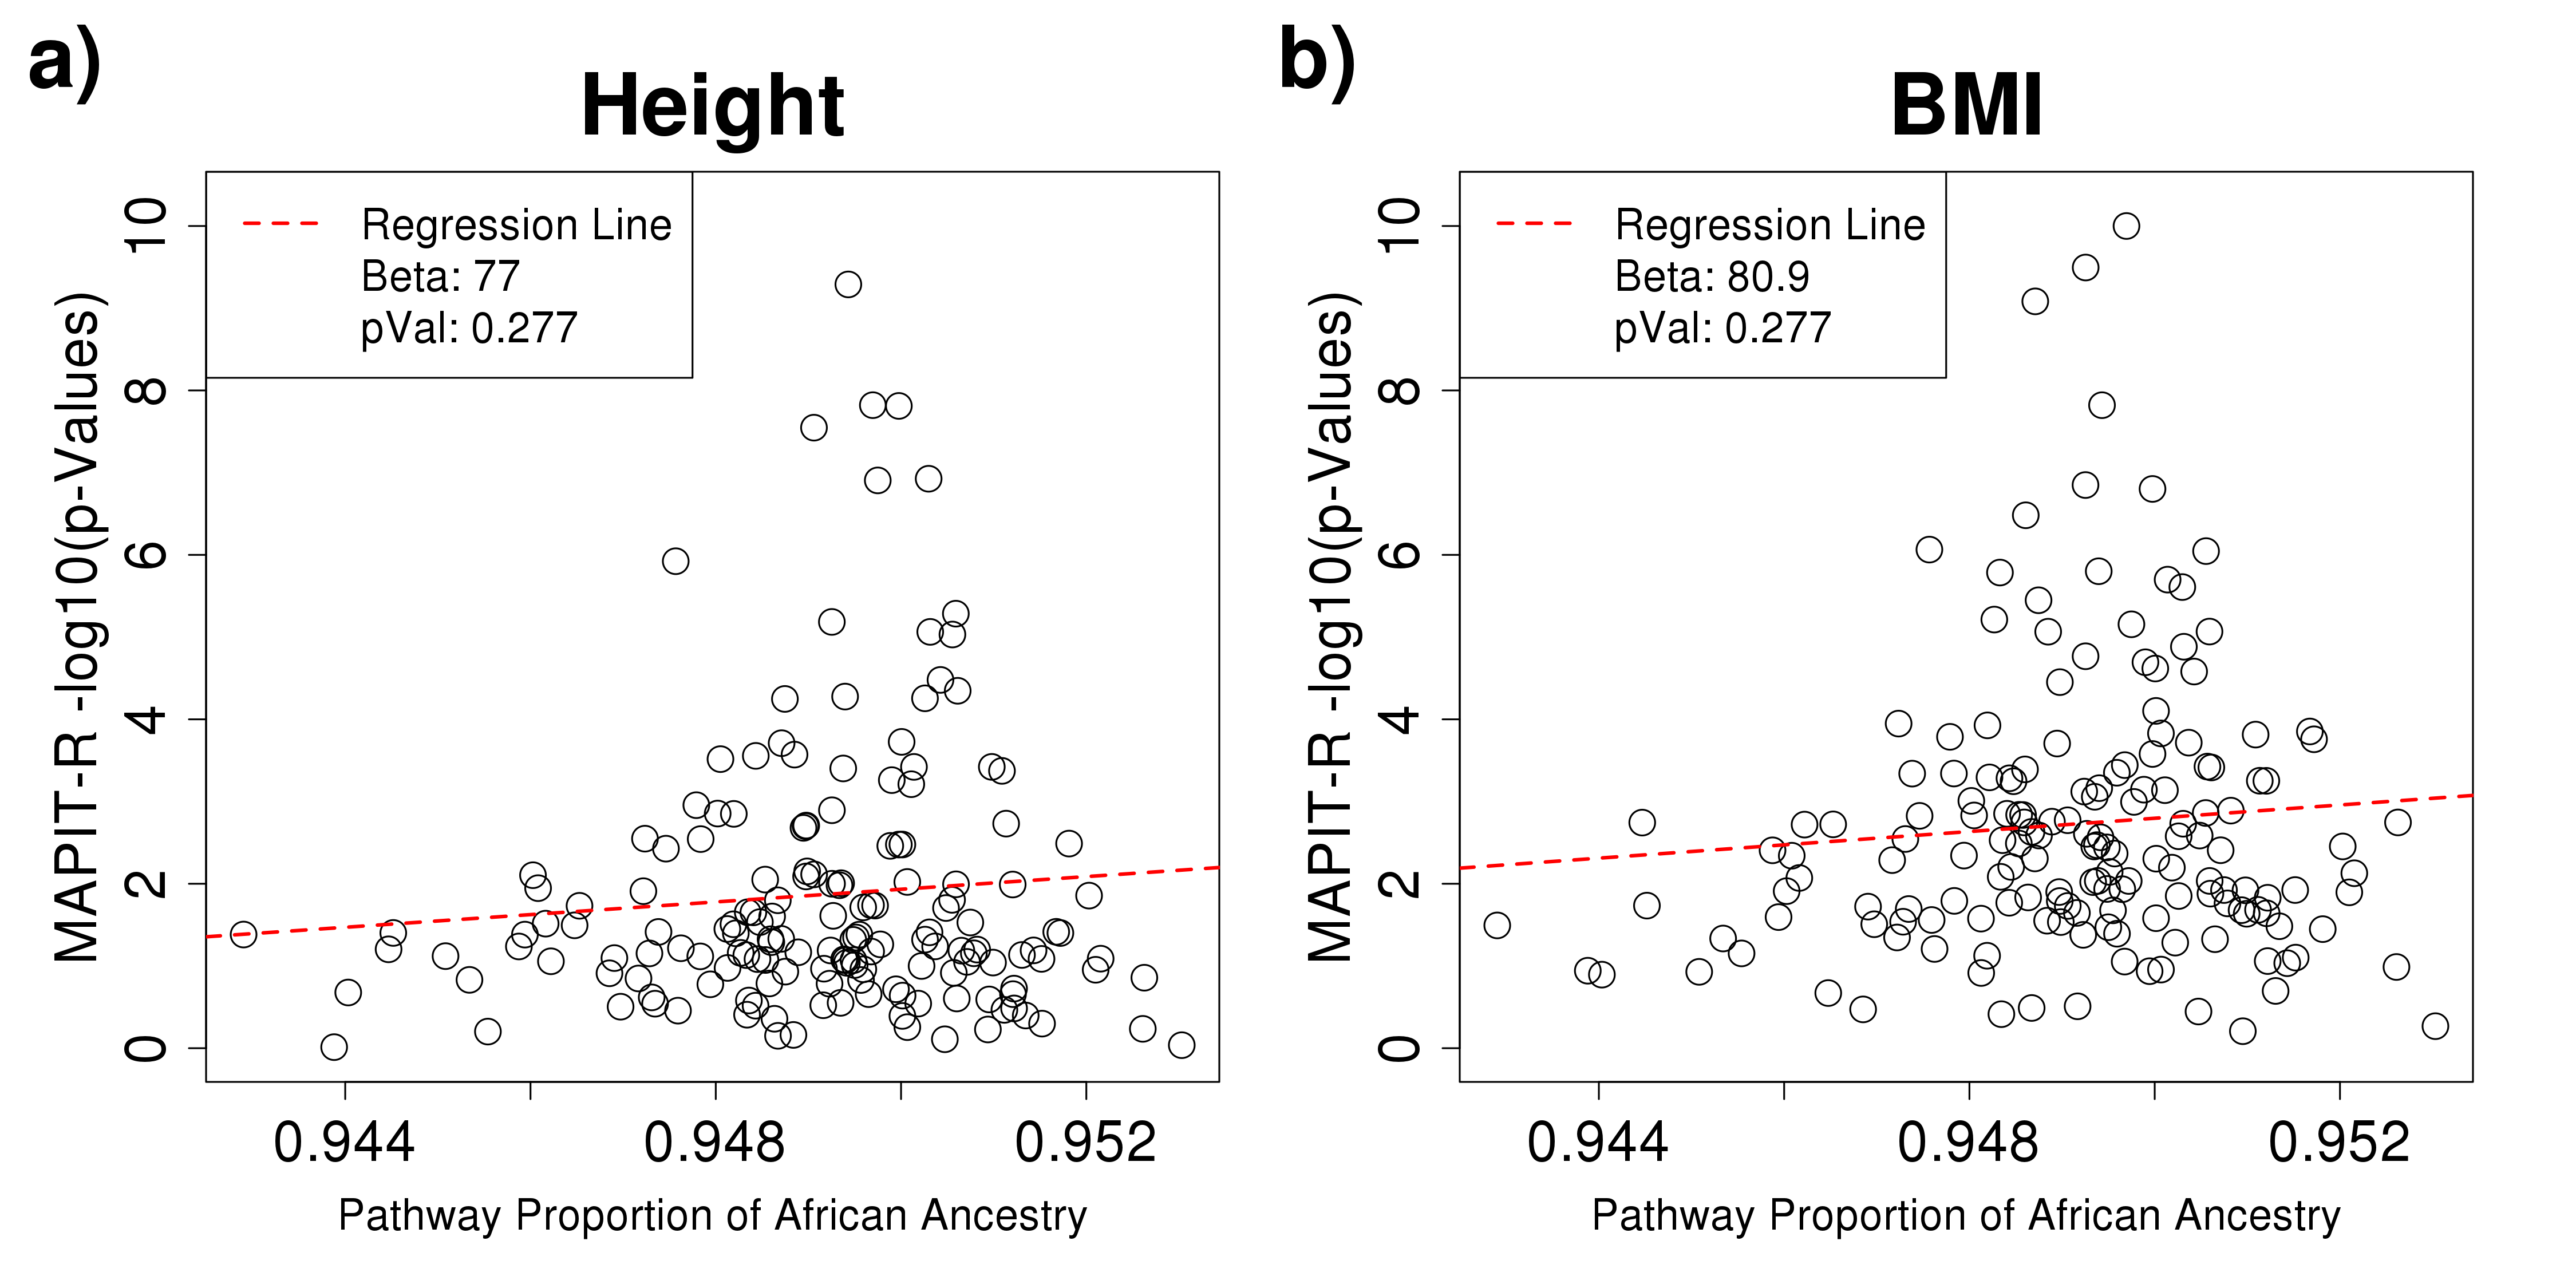
\includegraphics[scale=.35]{Images/Supp/InterPath_Supp_Figure_RFMix_vs2_African_KEGG_noHLA.png}
\caption[TBD]{\textbf{Pathway-level genetic diversity vs. MAPIT-R results in the African subgroup and KEGG database}. The figure shows the mean pairwise IBS proportions per pathway plotted against each pathway's MAPIT-R $p$-value for the African subgroup KEGG (a) height and (b) BMI analysis. IBS proportions were calculated per pathway by using each pathway's set of SNPs to derive pairwise IBS values between every set of individuals in the subgroup, and then averaging across each of these pairs for a final summary metric. Results with REACTOME database pathways can be found in Supplementary Figure \ref{InterPath-Main-Figure-RFMix-African-REACTOME}. We observe across the majority of our combinations no significant relationship between a pathway's mean pairwise IBS proportion and its MAPIT-R $p$-value.}
\label{InterPath-Supp-Figure-RFMix-African-KEGG}
\end{figure}
\clearpage

\setlength{\footskip}{3cm}
\begin{figure}[htbp]
\centering
\vspace*{-2cm}
\includegraphics[scale=.2]{Images/Supp/InterPath_Supp_Figure_PC1Loading_AllPaths_vs2_noHLA.png}
\caption[TBD]{\textbf{Relationship between MAPIT-R $p$-values and proportions of pathway SNPs loaded on PC1, all pathways}. Caption continued on next page.}
\label{InterPath-Supp-Figure-PC1Loading-AllPaths}
\end{figure}
\clearpage
\setlength{\footskip}{1cm}

\addtocounter{figure}{-1}
\begin{figure} [t!]
  \caption{\textbf{Relationship between MAPIT-R $p$-values and proportions of pathway SNPs loaded on PC1, all pathways}. The figure shows the proportion of SNPs within a given pathway that are strongly loaded on local PC1 plotted against that pathway's MAPIT-R -$\log_{10}$ $p$-value. All pathway sizes were used for this analysis. `Local' here refers to PCA having been conducted within-subgroup. SNPs are designated as `strongly loaded' on local PC1 if they are within the 10\% tails of the loading SNP score distributions. We observe that there is no significantly positive relationship between MAPIT-R $p$-values and proportion of SNPs that are strongly loaded on PC1 for any pathway database-phenotype-subgroup combination.}
\label{InterPath-Supp-Figure-PC1Loading-AllPaths-Caption}
\end{figure}
\clearpage

\setlength{\footskip}{2cm}
\begin{figure}[htbp]
\centering
\vspace*{-1.75cm}
\hspace*{-1cm}
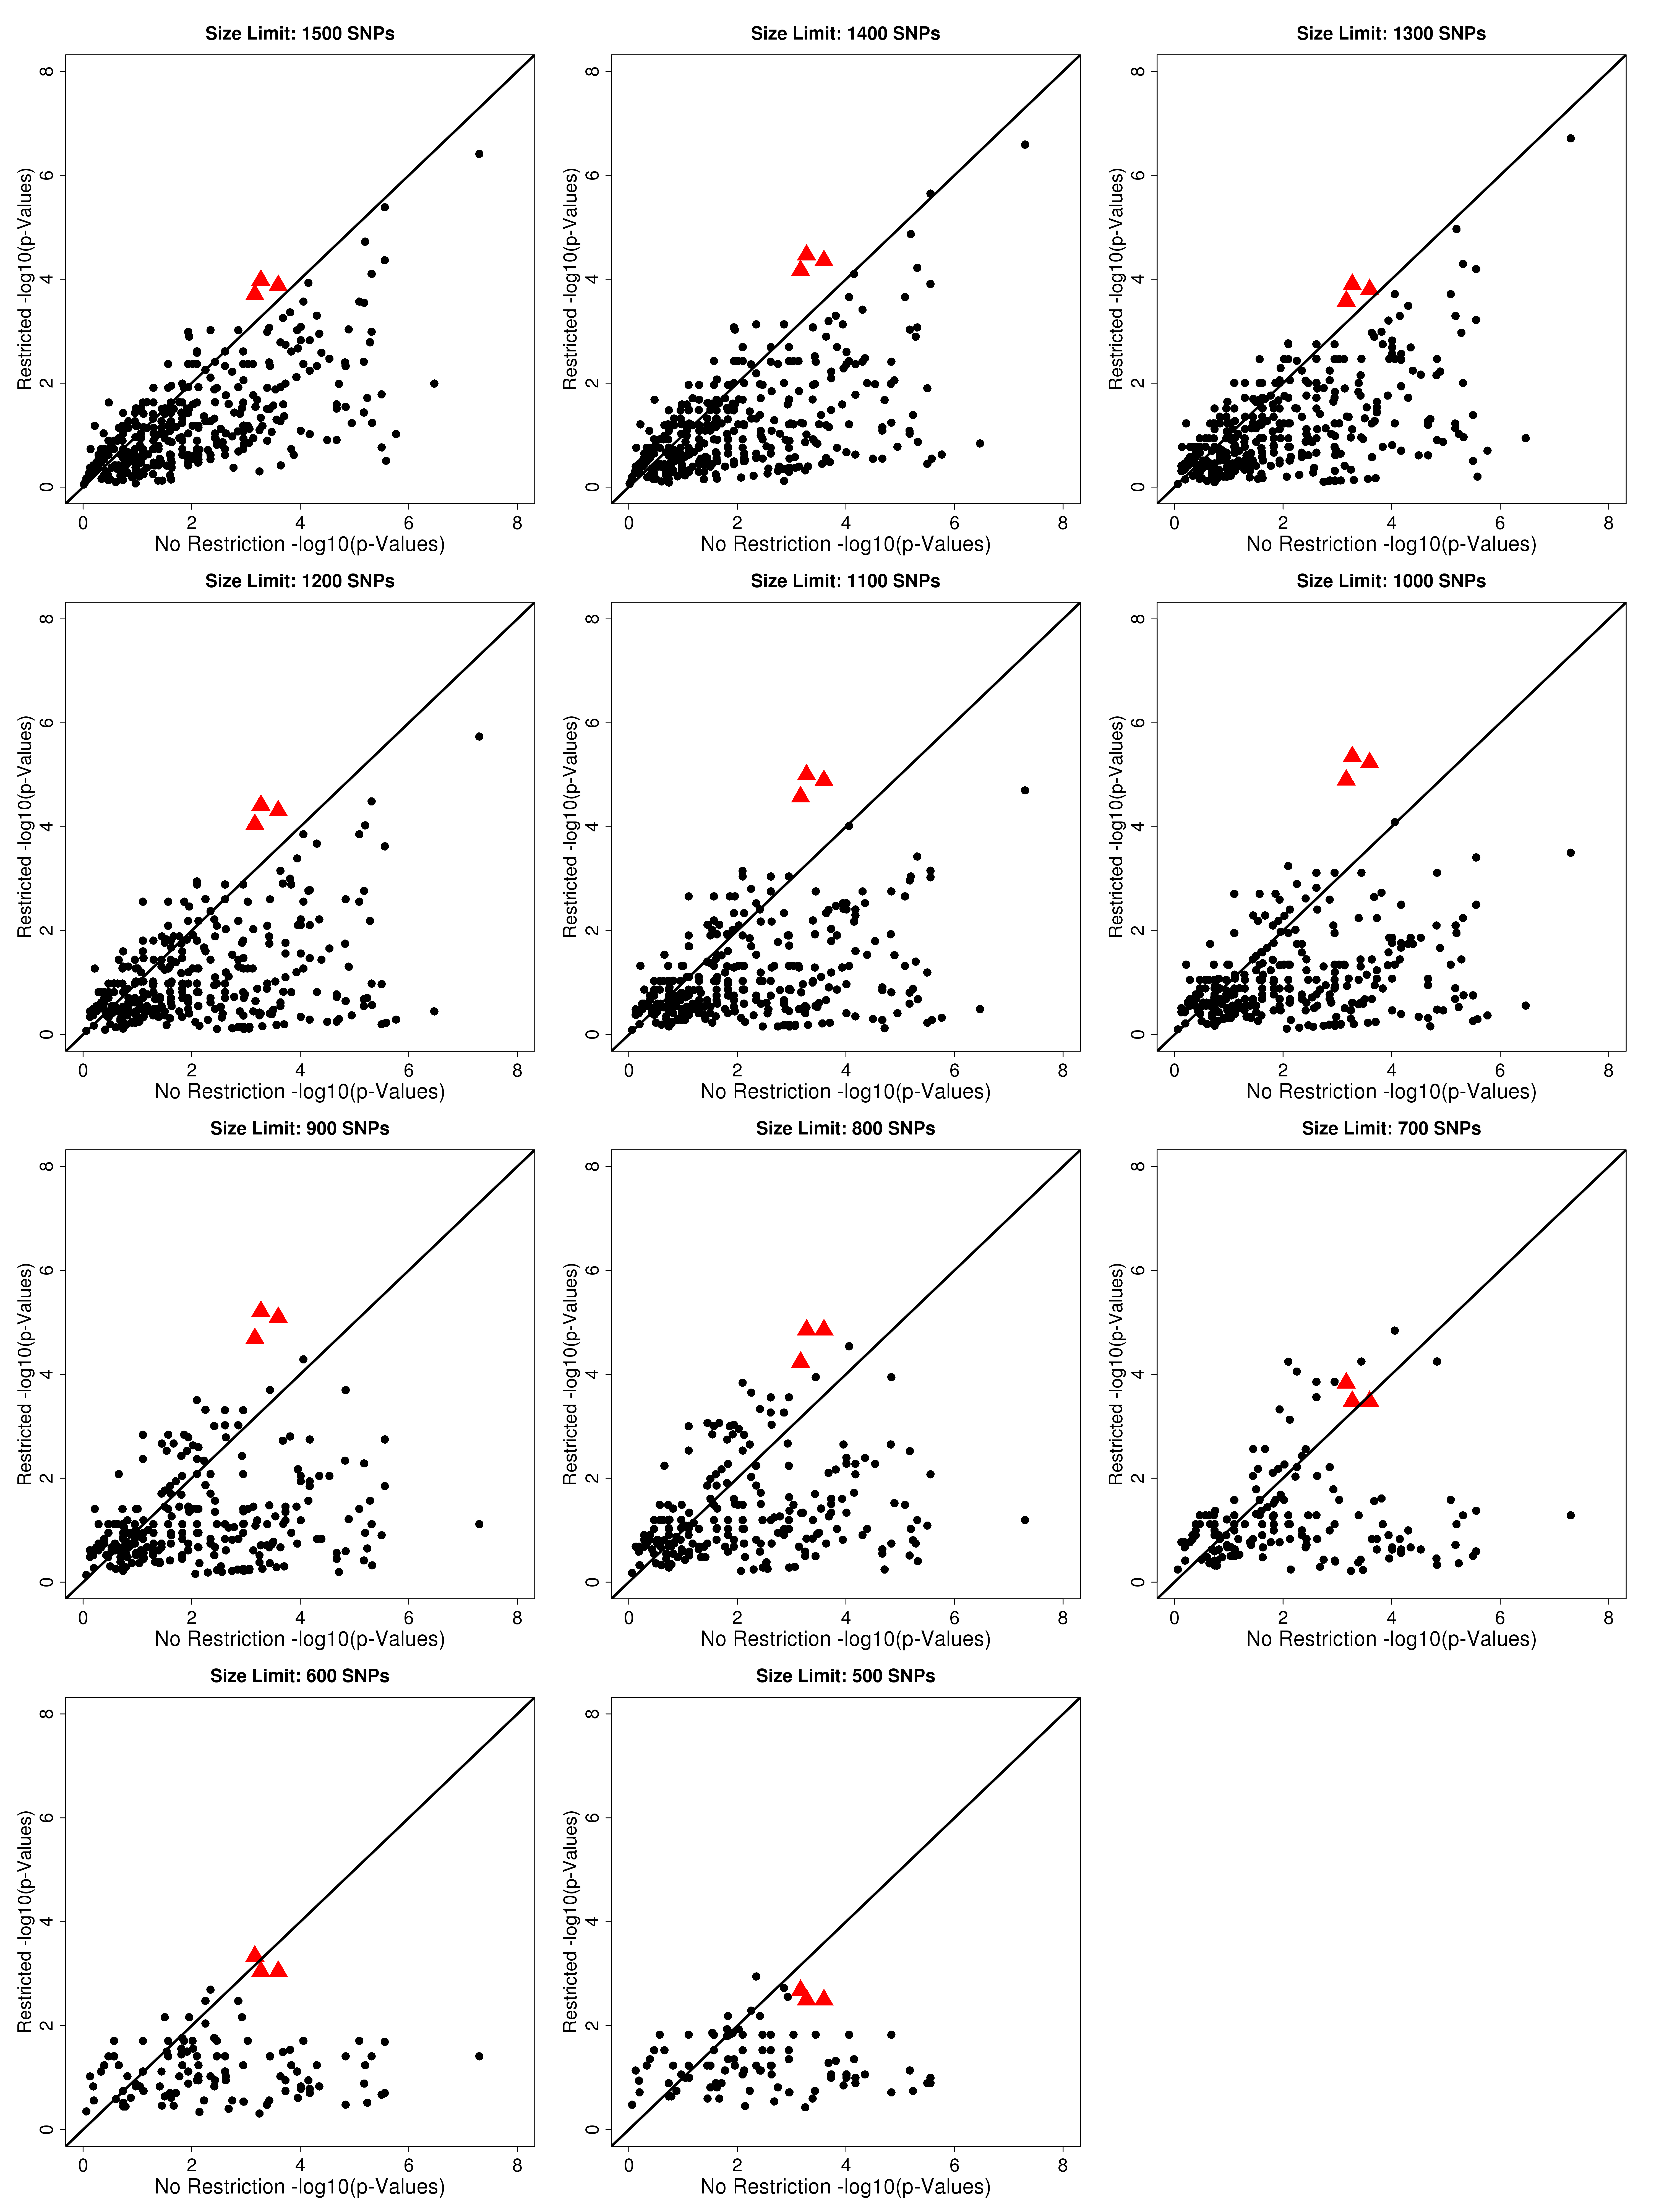
\includegraphics[scale=.325]{Images/Supp/InterPath_Supp_Figure_Hypergemeotric_SizeThresholds_vs1.png}
\caption[TBD]{\textbf{Impact of pathway size thresholds on hypergeometric enrichment analyses}. Caption continued on next page.}
\label{InterPath-Supp-Figure-Hypergeoemtric-SizeThresholds}
\end{figure}
\clearpage
\setlength{\footskip}{1cm}

\addtocounter{figure}{-1}
\begin{figure} [t!]
  \caption{\textbf{Impact of pathway size thresholds on hypergeometric enrichment analyses}. The figure shows multiple comparisons of size-restricted hypergeometric enrichment analyses versus unrestricted hypergeometric enrichment analyses using incrementally decreasing pathway size thresholds. Size thresholds change from 1,500 SNPs to 500 SNPs in 100 SNP increments. In each plot the $x$-axis is the unrestricted hypergeometric $p$-value for each gene and the $y$-axis is the size-restricted hypergeometric $p$-value for each gene. Red triangles represent results for each gene belonging to a proteasome gene family ({\emph{PSMA}}, {\emph{PSMB}}, {\emph{PSMC}}, {\emph{PSMD}}, {\emph{PSME}}, and {\emph{PSMF}}). Note that there are only three triangles since most proteasome genes are assigned to the same pathways.}
\label{InterPath-Supp-Figure-Hypergeoemtric-SizeThresholds-Caption}
\end{figure}
\clearpage

\section{Supplementary Tables}\label{Supplementary-Tables}

\begin{table}[ht]
\centering
\begin{tabular}{ccccc}
  \hline
\textbf{UK BioBank} & \textbf{Individuals} & \textbf{SNPs} & \textbf{KEGG} & \textbf{REACTOME} \\
\textbf{subgroup} & & & \textbf{Pathways} & \textbf{Pathways}  \\
  \hline
\textbf{Original subgroups:} & & & & \\
African & 3111 & 374466 & 180 & 658 \\ 
British.Ran4000 & 3848 & 600006 & 173 & 650 \\ 
Caribbean & 3833 & 410017 & 181 & 661 \\ 
Chinese & 1448 & 345221 & 153 & 626 \\ 
Indian & 5077 & 505854 & 181 & 662 \\ 
Pakistani & 1581 & 516806 & 141 & 596 \\ 
\\
\textbf{British Replicates:} & & & & \\
British.Ran4000.2 & 3869 & 599381 & 173 & 650 \\ 
British.Ran4000.3 & 3836 & 600654 & 173 & 649 \\ 
British.Ran4000.4 & 3838 & 599829 & 173 & 650 \\ 
British.Ran4000.5 & 3853 & 599442 & 173 & 650 \\ 
British.Ran10000 & 9603 & 597298 & 186 & 669 \\ 
British.Ran10000.2 & 9628 & 597577 & 186 & 669 \\ 
British.Ran10000.3 & 9636 & 597486 & 186 & 669 \\ 
British.Ran10000.4 & 9593 & 597369 & 186 & 669 \\ 
British.Ran10000.5 & 9596 & 597507 & 186 & 669 \\ 
  \hline
\end{tabular}
\caption[TBD]{\textbf{Pathways and subgroups of the UK BioBank analyzed in this study}. The table shows the individual, SNP, and pathway counts for each of the UKB subgroups analyzed in this study. `Original subgroups' refers to the multiple global human ancestries that were initially analyzed at the beginning of this study, and `British Replicates' refers specifically to the subgroups that were created to analyze multiple, independent random subsamples of the UKB British cohort. The number of individuals and SNPs post quality-control are shown in the second and third columns (see Materials and Methods), and the number of KEGG and REACTOME pathways analyzed in each subgroup are shown in the fourth and fifth columns. Note that for the `British Replicates' subgroups each group began with an independent set of either 4,000 or 10,000 individuals from the original UKB phenotype file.}
\label{InterPath-Supp-Table-UKBPopStats}
\end{table}
\clearpage

%Irish & 11575 & 588324 & 186 & 671 \\ 

%\textbf{Supplementary Tables 2a-d.} \textbf{Lists of New \bmass{} Multivariate Associations, per Dataset}. \\ Attached Excel sheets list new \bmass{} associations for each dataset analyzed.
%\bigskip \bigskip

\begin{table} [t!]
  \caption{\textbf{Lists of genome-wide significant MAPIT-R pathways, per subgroup}.  Attached Excel sheets list the pathways that were found to be MAPIT-R genome-wide significant in each UKB subgroup for the following phenotype and pathway database combinations: (a) KEGG+Height, (b) KEGG+BMI, (c) REACTOME+Height, and (d) REACTOME+BMI. Genome-wide significance was determined by using a Bonferroni-corrected $p$-value threshold of .05 divided by the number of pathways tested (Supplementary Table \ref{InterPath-Supp-Table-UKBPopStats}).}
\label{InterPath-Supp-Table-TopPathways-AllPaths-AllPhenos}
\end{table}
\clearpage

\setlength{\footskip}{4cm}
\begin{landscape}
\begin{table}[ht]
\vspace*{-1.5cm}
\centering
\hspace*{-3.5cm}
\begin{tabular}{ccccccccc}
  \hline
\textbf{Population} & \textbf{Pathway} & \textbf{Bonferroni} & \textbf{Bonferroni} & \textbf{Bonferroni} & \multicolumn{2}{c}{\textbf{.001 Threshold}} & \multicolumn{2}{c}{\textbf{.01 Threshold}} \\
\cline{6-7}
\cline{8-9}
 & \textbf{Counts} & \textbf{Threshold} & \textbf{Counts} & \textbf{FDR} & \textbf{Counts} & \textbf{FDR} & \textbf{Counts} & \textbf{FDR} \\ 
  \hline
\textbf{KEGG Height:} & & & & & & & \\
African & 1800 & 2.778E-04 & 0 & 0.000  & 1 & 0.056 & 10 & 0.556 \\ 
  British.Ran4000 & 1730 & 2.890E-04 & 0 & 0.000 & 0 & 0.000 & 13 & 0.751 \\ 
  Caribbean & 1810 & 2.762E-04 & 1 & 0.055 & 1 & 0.055 & 5 & 0.276 \\ 
  Chinese & 1530 & 3.268E-04 & 0 & 0.000 & 3 & 0.196 & 24 & 1.569 \\ 
  Indian & 1810 & 2.762E-04 & 1 & 0.055 & 1 & 0.055 & 20 & 1.105 \\ 
  Pakistani & 1410 & 3.546E-04 & 0 & 0.000 & 2 & 0.142 & 17 & 1.206 \\ 
  \\
  \textbf{KEGG BMI:} & & & & & & & \\
African & 1800 & 2.778E-04 & 0 & 0.000 & 1 & 0.056 & 10 & 0.556 \\ 
  British.Ran4000 & 1730 & 2.890E-04 & 0 & 0.000 & 0 & 0.000 & 13 & 0.751 \\ 
  Caribbean & 1810 & 2.762E-04 & 1 & 0.055 & 1 & 0.055 & 5 & 0.276 \\ 
  Chinese & 1530 & 3.268E-04 & 0 & 0.000 & 3 & 0.196 & 24 & 1.569 \\ 
  Indian & 1810 & 2.762E-04 & 1 & 0.055 & 1 & 0.055 & 20 & 1.105 \\ 
  Pakistani & 1410 & 3.546E-04 & 0 & 0.000 & 2 & 0.142 & 17 & 1.206 \\ 
  \\
  \textbf{REACTOME Height:} & & & & & & & \\
  African & 1800 & 2.778E-04 & 0 & 0.000 & 1 & 0.056 & 16 & 0.889 \\
  British.Ran4000 & 1730 & 2.890E-04 & 1 & 0.058 & 2 & 0.116 & 14 & 0.809 \\
  Caribbean & 1810 & 2.762E-04 & 0 & 0.000 & 1 & 0.055 & 25 & 1.381 \\
  Chinese & 1530 & 3.268E-04 & 0 & 0.000 & 1 & 0.065 & 24 & 1.569 \\
  Indian & 1810 & 2.762E-04 & 1 & 0.055 & 2 & 0.110 & 20 & 1.105 \\
  Pakistani & 1410 & 3.546E-04 & 0 & 0.000 & 2 & 0.142 & 15 & 1.064 \\
  \\
  \textbf{REACTOME BMI:} & & & & & & & \\
African & 6580 & 7.599E-05 & 1 & 0.015 & 4 & 0.061 & 39 & 0.593 \\
  British.Ran4000 & 6490 & 7.704E-05 & 1 & 0.015 & 4 & 0.062 & 52 & 0.801 \\
  Caribbean & 6610 & 7.564E-05 & 0 & 0.000 & 13 & 0.197 & 97 & 1.467 \\
  Chinese & 6260 & 7.987E-05 & 0 & 0.000 & 6 & 0.096 & 49 & 0.783 \\
  Indian & 6620 & 7.553E-05 & 0 & 0.000 & 3 & 0.045 & 66 & 0.997 \\
  Pakistani & 5960 & 8.389E-05 & 0 & 0.000 & 4 & 0.067 & 45 & 0.755 \\
   \hline
\end{tabular}
\caption[TBD]{\textbf{MAPIT-R false discovery rates at different significance thresholds, per subgroup}. Caption continued on next page. }
\label{InterPath-Supp-Table-AllPops-FDRs}
\end{table}
\end{landscape}
\clearpage
\setlength{\footskip}{1cm}

\addtocounter{table}{-1}
\begin{table} [t!]
  \caption{\textbf{MAPIT-R false discovery rates at different significance thresholds, per subgroup}. The table shows for various significance thresholds the false discovery rates observed from MAPIT-R when run on ten rounds of phenotype permutations for each UKB subgroup and pathway database. The first column lists the pathway database-phenotype-UKB subgroup combinations. The second column lists the total number of pathways that were tested across each of the ten phenotype permutations. The third column shows the $p$-value threshold associated with using the Bonferroni method of correction, also known as the `genome-wide significant' threshold. The fourth column shows the number of pathways across all ten phenotype permutation rounds that crossed this Bonferroni threshold. The fifth column shows the associated FDR associated with the fourth column. And the remaining six columns show the same setup as columns three to five but with a $p$-value threshold of either 0.001 or 0.01.}
\label{InterPath-Supp-Table-AllPops-FDRs-Caption}
\end{table}
\clearpage

\setlength{\footskip}{2cm}
\begin{landscape}
\begin{table}[ht]
\centering
\begin{tabular}{ll}
  \hline
 \textbf{Population} & \textbf{Pathways}\\
 \textbf{Comparison} & \\
  \hline
\textbf{African Vs.} & \\
\textbf{Caribbean:} & \\
 & KEGG\_ARRHYTHMOGENIC\_RIGHT\_VENTRICULAR\_CARDIOMYOPATHY\_ARVC \\
 & KEGG\_AXON\_GUIDANCE \\
 & KEGG\_CHEMOKINE\_SIGNALING\_PATHWAY \\
 & KEGG\_HYPERTROPHIC\_CARDIOMYOPATHY\_HCM \\
 & KEGG\_NATURAL\_KILLER\_CELL\_MEDIATED\_CYTOTOXICITY \\
 & KEGG\_VASCULAR\_SMOOTH\_MUSCLE\_CONTRACTION \\
\\
\textbf{African Vs.} & \\
\textbf{Chinese:} & \\
 & KEGG\_ALLOGRAFT\_REJECTION \\
 & KEGG\_ANTIGEN\_PROCESSING\_AND\_PRESENTATION \\
 & KEGG\_GRAFT\_VERSUS\_HOST\_DISEASE \\
 & KEGG\_SYSTEMIC\_LUPUS\_ERYTHEMATOSUS \\
 & KEGG\_TYPE\_I\_DIABETES\_MELLITUS \\
   \hline
\end{tabular}
\caption[TBD]{\textbf{Genome-wide significant MAPIT-R KEGG pathway overlap between UKB subgroups, in height}. Caption continued on next page. }
\label{InterPath-Supp-Table-MAPITR-TopPathway-Overlap}
\end{table}
\end{landscape}
\clearpage
\setlength{\footskip}{1cm}

\addtocounter{table}{-1}
\begin{table} [t!]
  \caption{\textbf{Genome-wide significant MAPIT-R KEGG pathway overlap between UKB subgroups, in height}. The table shows genome-wide significant pathways that overlap between multiple UKB subgroups. Specifically, pathways that overlap between the African subgroup and Caribbean subgroup, and between the African subgroup and Chinese subgroup, are listed for height results from KEGG.}
\label{InterPath-Supp-Table-MAPITR-TopPathway-Overlap-Caption}
\end{table}
\clearpage

\setlength{\footskip}{2cm}
\begin{table}[ht]
\centering
\begin{tabular}{lll}
  \hline
 \textbf{Population} & \textbf{Gene} & \textbf{Genes} \\
 \textbf{Comparison} & \textbf{Count} & \\
  \hline
\textbf{African Vs.} & & \\
\textbf{Caribbean:} & & \\
& 4 & MAPK3,MAPK1 \\
& 3 & ROCK2,ROCK1,RHOA,RAF1,RAC2,RAC1,PRKCB, \\
& & PAK1,NRAS,MAP2K1,KRAS,ITGB1,HRAS,CACNA1S, \\
& & CACNA1D,CACNA1C,BRAF \\
\\
\textbf{African Vs.} & & \\
\textbf{Chinese:} & & \\
& 5 & HLA-DRB1,HLA-DRA,HLA-DQB1,HLA-DQA2,HLA-DQA1, \\
& & HLA-DPB1,HLA-DPA1,HLA-DOB,HLA-DOA,HLA-DMB, \\
& & HLA-DMA \\
& 4 & TNF,IFNG,HLA-G,HLA-F,HLA-E,HLA-C,HLA-B,HLA-A, \\ 
& & CD86,CD80,CD28 \\
& 3 & PRF1,IL2,GZMB,FASLG,FAS \\
   \hline
\end{tabular}
\caption[TBD]{\textbf{Gene counts across genome-wide significant MAPIT-R KEGG pathways that overlap between UKB subgroups, in height}. The table shows genes that are present across multiple pathways that overlap between the population subgroups referenced in the first column. Pathways from which these gene count lists are derived can be found in Supplementary Table \ref{InterPath-Supp-Table-MAPITR-TopPathway-Overlap}. The second column lists the number of times the given genes appear across the aforementioned lists of pathways. The third column lists the specific genes the appear at the specific gene count numbers. Note that these results are specifically for the KEGG height analysis.}
\label{InterPath-Supp-Table-MAPITR-TopPathway-GeneCounts-Overlap}
\end{table}
\clearpage
\setlength{\footskip}{1cm}

\begin{table}[ht]
\centering
\begin{tabular}{cl}
  \hline
 \textbf{Frequency} & \textbf{Genes} \\
  \hline
  4 & PIK3R5,PIK3R3,PIK3R2,PIK3R1,PIK3CG,PIK3CD,PIK3CB, \\
  & PIK3CA,AKT3,AKT2,AKT1 \\
  3 & SOS2,SOS1,RAF1,PLCG1,NRAS,MAPK3,MAPK1,MAP2K2, \\
  & MAP2K1,KRAS,HRAS,GRB2,CDK4 \\
  2 & TP53,TGFA,RXRG,RXRB,RXRA,RELA,RB1,RARB,PTK2, \\
  & PRKCG,PRKCB,PRKCA,PLCG2,PDPK1,PAK6,PAK4,PAK2, \\
  & PAK1,NFKBIA,NFKB1,NCK2,NCK1,MYC,MAPK9,MAP2K7, \\ 
  & JUN,IKBKB,GSK3B,FHIT,ERBB2,EGFR,EGF,E2F3,E2F2, \\
  & E2F1,CHUK,CDKN1B,CDK6,CCND1,CBLC,CBLB,CBL, \\
  & CASP9,BRAF,BAD \\
   \hline
\end{tabular}
\caption[TBD]{\textbf{Gene counts across four KEGG pathways highlighted in African height vs. BMI analysis (Figure \ref{InterPath-Main-Figure-MAPITR-PhenoComps-African})}. The table shows the genes that are present across multiple of the pathways highlighted in blue in Figure \ref{InterPath-Main-Figure-MAPITR-PhenoComps-African}; these are pathways that have particularly more significant MAPIT-R $p$-values in BMI than in height. The first column lists the frequency (out of four) the given genes appear across the aforementioned list of pathways in Figure \ref{InterPath-Main-Figure-MAPITR-PhenoComps-African}. The second column lists the specific genes that appear at the given frequency across the four pathways highlighted in Figure \ref{InterPath-Main-Figure-MAPITR-PhenoComps-African}.}
\label{InterPath-Supp-Table-MAPITR-PhenoComps-African-GeneCounts}
\end{table}
\clearpage

\begin{table} [t!]
  \caption{\textbf{Gene counts across MAPIT-R genome-wide significant pathways, per subgroup}. Attached Excel sheets contain lists of genes that appear multiple times across the MAPIT-R genome-wide significant pathways in each UKB subgroup for the following pathway database-phenotype combinations: (a) KEGG-Height, (b) KEGG-BMI, (c) REACTOME-Height, and (d) REACTOME-BMI. Genome-wide significance was determined by using a Bonferroni-corrected $p$-value threshold of .05 divided by the number of pathways tested (Supplementary Table \ref{InterPath-Supp-Table-UKBPopStats}).}
\label{InterPath-Supp-Table-AllPops-TopGeneCounts-Caption}
\end{table}

\begin{table} [t!]
  \caption{\textbf{Gene counts across size-restricted MAPIT-R genome-wide significant pathways, per subgroup}. Attached Excel sheets contain lists of genes that appear multiple times across the MAPIT-R genome-wide significant pathways that contain less than or equal to 1,000 SNPs (`size-restricted') in each UKB subgroup for the following pathway database-phenotype combinations: (a) KEGG-Height, (b) KEGG-BMI, (c) REACTOME-Height, and (d) REACTOME-BMI. Genome-wide significance was determined by using a Bonferroni-corrected $p$-value threshold of .05 divided by the number of pathways tested (Supplementary Table \ref{InterPath-Supp-Table-UKBPopStats}).}
\label{InterPath-Supp-Table-AllPops-TopGeneCounts-SizeRestricted-Caption}
\end{table}
\clearpage

\begin{table} [t!]
  \caption{\textbf{Results from original and size-restricted hypergeometric tests in BMI-African, per gene.}. Attached Excel sheets contain lists of the hypergeometric -$\log_{10}$ $p$-values for both the original and size-restricted gene count analyses per gene in both the KEGG and REACTOME-BMI-African combinations. Differences in the -$\log_{10}$ $p$-values between the original and size-restricted hypergeometric analyses are also shown per gene. Plots of these differences in -$\log_{10}$ $p$-values can be seen in Figure \ref{InterPath-Main-Figure-Hypergeometric-RestrictedComps-African-BMI}.}
\label{InterPath-Supp-Table-Hypergeometric-RestrictedComps-African-BMI}
\end{table}
\clearpage

\begin{landscape}
\begin{table}[ht]
\centering
\hspace*{-1.5cm}
\begin{tabular}{ccccccc}
  \hline
  \textbf{Gene} & \textbf{Pathway SNP} & \textbf{Gene Count in} & \textbf{Total Count of} & \textbf{Gene Count in} & \textbf{Total Count of} & \textbf{Hypergeometric} \\
   & \textbf{Count Limit} & \textbf{Top Pathways} & \textbf{Top Pathways} & \textbf{All Pathways} & \textbf{All Pathways} & \textbf{$p$-Value} \\
  \hline
 \textbf{UBA52} & & & & & & \\
 & No Limit & 22 & 65 & 106 & 658 & 1.537E-4 \\
 & $<$ 1000 SNPs & 10 & 26 & 84 & 577 & 1.855E-3 \\
\\
 \textbf{PSM*} & & & & & & \\
 & No Limit & 12 & 65 & 44 & 658 & 5.304E-4 \\
 & $<$ 1000 SNPs & 9 & 26 & 34 & 577 & 4.464E-6 \\
   \hline
\end{tabular}
\caption[TBD]{\textbf{MAPIT-R Genome-Wide Significant Pathway Gene Counts: Hypergeometric Enrichment Examples}. Caption continued on next page.}
\label{InterPath-Supp-Table-AllPops-TopGeneCount-HypergeometricTests}
\end{table}
\end{landscape}
\clearpage

\addtocounter{table}{-1}
\begin{table} [t!]
  \caption{\textbf{PSM* and UBA52 gene count enrichment test examples, size restriction and no restriction}. The table shows examples and results of running the hypergeometric test for enrichment on two different genes in two different study designs. In all cases a gene is tested for being significantly more frequent among the set of MAPIT-R genome-wide significant pathways than among the background distribution of pathways in the original database. Two study designs were employed for these tests, either (a) using all pathways present in the given databases or (b) using only pathways that contained less than or equal to 1,000 SNPs. The first column lists the gene or gene family being tested. The second column lists which of the two aforementioned study designs was used. Columns three through six list the different count values used in the hypergeometric test: the third column lists the number of times a gene is present among the genome-wide significant list of pathways, the fourth column lists the total number of pathways that were genome-wide significant, the fifth column lists the number of times a gene is present among all the pathways in the given database, and the sixth column lists the total number of pathways in the given database. The seventh column is the hypergeometric $p$-value associated with columns three through six. Note that the vast majority of proteasome genes included in our analysis had the same number of gene counts across each hypergeometric category, hence why \textbf{PSM*} was used to represent them as a whole.}
\label{InterPath-Supp-Table-AllPops-TopGeneCount-HypergeometricTests-Caption}
\end{table}
\clearpage

\begin{table} [t!]
  \caption{\textbf{MAPIT-R $p$-values from rerunning REACTOME pathways + BMI with each proteasome gene family individually removed, per subgroup}. Attached Excel sheets contain the MAPIT-R $p$-values for each of the REACTOME pathways analyzed in Figure \ref{InterPath-Main-Figure-Proteasome-Panels} + BMI with each of the proteasome gene families (eg \textit{PSMA}, \textit{PSMB}, \textit{PSMC}, \textit{PSMD}, \textit{PSME}, and \textit{PSMF}) removed one at a time, per UKB subgroup. These are the raw MAPIT-R $p$-values underlying Figure \ref{InterPath-Main-Figure-Proteasome-Panels} and Supplementary Figures \ref{InterPath-Supp-Figure-Prot-Heatplots-African}\textcolor{blue}{-f}. Note that for some subgroups not all of the original pathways from Figure \ref{InterPath-Main-Figure-Proteasome-Panels} were analyzable (generally due to number of SNPs >> number of individuals).}
\label{InterPath-Supp-Table-AllPops-Proteasome-Dropouts-Caption}
\end{table}
\clearpage

\setlength{\footskip}{4cm}
\begin{landscape}
\begin{table}[ht]
\vspace*{-1.25cm}
\centering
\hspace*{-3.25cm}
\begin{tabular}{ccccccccccc}
  \hline
\textbf{Population} & \textbf{Pathway} & \textbf{Bonferroni} & \textbf{Bonferroni} & \textbf{Bonferroni} & \textbf{0.001} & \textbf{0.001} & \textbf{0.001} & \textbf{0.01} & \textbf{0.01} & \textbf{0.01} \\
 & \textbf{Counts} & \textbf{Threshold} & \textbf{Counts} & \textbf{FDR} & \textbf{Threshold} & \textbf{Counts} & \textbf{FDR} & \textbf{Threshold} & \textbf{Counts} & \textbf{FDR} \\ 
  \hline
\textbf{KEGG Height:} & & & & & & & & & \\
British.Ran4000 & 1730 & 2.890E-04 & 0 & 0.000 & 0.001 & 0 & 0.000 & 0.010 & 13 & 0.751 \\
  British.Ran4000.2 & 1730 & 2.890E-04 & 0 & 0.000 & 0.001 & 1 & 0.058 & 0.010 & 18 & 1.040 \\
  British.Ran4000.3 & 1730 & 2.890E-04 & 1 & 0.058 & 0.001 & 1 & 0.058 & 0.010 & 20 & 1.156 \\
  British.Ran4000.4 & 1730 & 2.890E-04 & 0 & 0.000 & 0.001 & 4 & 0.231 & 0.010 & 23 & 1.329 \\
  British.Ran4000.5 & 1730 & 2.890E-04 & 0 & 0.000 & 0.001 & 2 & 0.116 & 0.010 & 22 & 1.272 \\
  British.Ran10000.1 & 1860 & 2.688E-04 & 0 & 0.000 & 0.001 & 1 & 0.054 & 0.010 & 26 & 1.398 \\
  British.Ran10000.2 & 1860 & 2.688E-04 & 0 & 0.000 & 0.001 & 1 & 0.054 & 0.010 & 12 & 0.645 \\
  British.Ran10000.3 & 1860 & 2.688E-04 & 2 & 0.108 & 0.001 & 2 & 0.108 & 0.010 & 21 & 1.129 \\
  British.Ran10000.4 & 1860 & 2.688E-04 & 1 & 0.054 & 0.001 & 2 & 0.108 & 0.010 & 16 & 0.860 \\
  British.Ran10000.5 & 1860 & 2.688E-04 & 0 & 0.000 & 0.001 & 0 & 0.000 & 0.010 & 12 & 0.645 \\
  \\
  \textbf{KEGG BMI:} & & & & & & & & & \\
British.Ran4000 & 1730 & 2.890E-04 & 1 & 0.058 & 0.001 & 2 & 0.116 & 0.010 & 14 & 0.809 \\
  British.Ran4000.2 & 1730 & 2.890E-04 & 0 & 0.000 & 0.001 & 1 & 0.058 & 0.010 & 23 & 1.329 \\
  British.Ran4000.3 & 1730 & 2.890E-04 & 0 & 0.000 & 0.001 & 3 & 0.173 & 0.010 & 21 & 1.214 \\
  British.Ran4000.4 & 1730 & 2.890E-04 & 1 & 0.058 & 0.001 & 5 & 0.289 & 0.010 & 21 & 1.214 \\
  British.Ran4000.5 & 1730 & 2.890E-04 & 2 & 0.116 & 0.001 & 7 & 0.405 & 0.010 & 23 & 1.329 \\
  British.Ran10000.1 & 1860 & 2.688E-04 & 0 & 0.000 & 0.001 & 1 & 0.054 & 0.010 & 25 & 1.344 \\
  British.Ran10000.2 & 1860 & 2.688E-04 & 2 & 0.108 & 0.001 & 4 & 0.215 & 0.010 & 22 & 1.183 \\
  British.Ran10000.3 & 1860 & 2.688E-04 & 0 & 0.000 & 0.001 & 2 & 0.108 & 0.010 & 20 & 1.075 \\
  British.Ran10000.4 & 1860 & 2.688E-04 & 1 & 0.054 & 0.001 & 2 & 0.108 & 0.010 & 23 & 1.237 \\
  British.Ran10000.5 & 1860 & 2.688E-04 & 0 & 0.000 & 0.001 & 0 & 0.000 & 0.010 & 20 & 1.075 \\
   \hline
\end{tabular}
\caption[TBD]{\textbf{MAPIT-R false discovery rates at different significance thresholds, per British replicate}. Caption continued at end of tables.}
\label{InterPath-Supp-Table-BritReps-FDRs-pt1}
\end{table}
\end{landscape}
\clearpage
\setlength{\footskip}{1cm}
\addtocounter{table}{-1}

\setlength{\footskip}{4cm}
\renewcommand{\thetable}{\arabic{table}}
\begin{landscape}
\begin{table}[ht]
\vspace*{-1.25cm}
\centering
\hspace*{-3.5cm}
\begin{tabular}{ccccccccccc}
  \hline
\textbf{Population} & \textbf{Pathway} & \textbf{Bonferroni} & \textbf{Bonferroni} & \textbf{Bonferroni} & \textbf{0.001} & \textbf{0.001} & \textbf{0.001} & \textbf{0.01} & \textbf{0.01} & \textbf{0.01} \\
 & \textbf{Counts} & \textbf{Threshold} & \textbf{Counts} & \textbf{FDR} & \textbf{Threshold} & \textbf{Counts} & \textbf{FDR} & \textbf{Threshold} & \textbf{Counts} & \textbf{FDR} \\ 
  \hline
  \textbf{REACTOME Height:} & & & & & & & & & \\
British.Ran4000 & 6500 & 7.692E-05 & 0 & 0.000 & 0.001 & 9 & 0.138 & 0.010 & 69 & 1.062 \\
  British.Ran4000.2 & 6500 & 7.692E-05 & 0 & 0.000 & 0.001 & 4 & 0.062 & 0.010 & 61 & 0.938 \\
  British.Ran4000.3 & 6490 & 7.704E-05 & 1 & 0.015 & 0.001 & 8 & 0.123 & 0.010 & 59 & 0.909 \\
  British.Ran4000.4 & 6500 & 7.692E-05 & 0 & 0.000 & 0.001 & 5 & 0.077 & 0.010 & 69 & 1.062 \\
  British.Ran4000.5 & 6500 & 7.692E-05 & 0 & 0.000 & 0.001 & 6 & 0.092 & 0.010 & 53 & 0.815 \\
   British.Ran10000.1 & 6690 & 7.474E-05 & 0 & 0.000 & 0.001 & 4 & 0.060 & 0.010 & 55 & 0.822 \\
  British.Ran10000.2 & 6690 & 7.474E-05 & 0 & 0.000 & 0.001 & 4 & 0.060 & 0.010 & 52 & 0.777 \\
  British.Ran10000.3 & 6690 & 7.474E-05 & 2 & 0.030 & 0.001 & 11 & 0.164 & 0.010 & 60 & 0.897 \\
  British.Ran10000.4 & 6690 & 7.474E-05 & 1 & 0.015 & 0.001 & 4 & 0.060 & 0.010 & 69 & 1.031 \\
  British.Ran10000.5 & 6690 & 7.474E-05 & 0 & 0.000 & 0.001 & 4 & 0.060 & 0.010 & 60 & 0.897 \\

  \\
  \textbf{REACTOME BMI:} & & & & & & & & & \\
British.Ran4000 & 6490 & 7.704E-05 & 1 & 0.015 & 0.001 & 4 & 0.062 & 0.010 & 52 & 0.801 \\
  British.Ran4000.2 & 6500 & 7.692E-05 & 1 & 0.015 & 0.001 & 14 & 0.215 & 0.010 & 63 & 0.969 \\
  British.Ran4000.3 & 6490 & 7.704E-05 & 0 & 0.000 & 0.001 & 5 & 0.077 & 0.010 & 79 & 1.217 \\
  British.Ran4000.4 & 6500 & 7.692E-05 & 2 & 0.031 & 0.001 & 6 & 0.092 & 0.010 & 61 & 0.938 \\
  British.Ran4000.5 & 6500 & 7.692E-05 & 0 & 0.000 & 0.001 & 7 & 0.108 & 0.010 & 73 & 1.123 \\
  British.Ran10000.1 & 6690 & 7.474E-05 & 2 & 0.030 & 0.001 & 10 & 0.149 & 0.010 & 73 & 1.091 \\
  British.Ran10000.2 & 6690 & 7.474E-05 & 0 & 0.000 & 0.001 & 3 & 0.045 & 0.010 & 42 & 0.628 \\
  British.Ran10000.3 & 6690 & 7.474E-05 & 1 & 0.015 & 0.001 & 10 & 0.149 & 0.010 & 74 & 1.106 \\
  British.Ran10000.4 & 6690 & 7.474E-05 & 0 & 0.000 & 0.001 & 7 & 0.105 & 0.010 & 65 & 0.972 \\
  British.Ran10000.5 & 6690 & 7.474E-05 & 0 & 0.000 & 0.001 & 5 & 0.075 & 0.010 & 57 & 0.852 \\
   \hline
\end{tabular}
\caption[TBD]{\textbf{MAPIT-R false discovery rates at different significance thresholds, per British replicate}. Continued.}
\label{InterPath-Supp-Table-BritReps-FDRs-pt2}
\end{table}
\end{landscape}
\clearpage
\setlength{\footskip}{1cm}

\addtocounter{table}{-1}
\begin{table} [t!]
  \caption{\textbf{MAPIT-R false discovery rates at different significance thresholds, per British replicate}. The tables show for various significance thresholds the false discovery rates observed from MAPIT-R when run on ten rounds of phenotype permutations for each British replicate subsample and pathway database. The first column lists the pathway database-phenotype-British replicate subsample combinations. The second column lists the total number of pathways that were tested across each of the ten phenotype permutations. The third column shows the $p$-value threshold associated with using the Bonferroni method of correction, also known as the `genome-wide significant' threshold. The fourth column shows the number of pathways across all ten phenotype permutation rounds that crossed this Bonferroni threshold. The fifth column shows the associated FDR associated with the fourth column. And the remaining six columns show the same setup as columns three to five but with a $p$-value threshold of either 0.001 or 0.01.}
\label{InterPath-Supp-Table-BritReps-FDRs-Caption}
\end{table}
\clearpage

\setlength{\footskip}{3.5cm}
\begin{landscape}
\begin{table}[ht]
\centering
\vspace{-1cm}
\hspace*{-2.5cm}
\begin{tabular}{ccccccccc}
  \hline
  \multicolumn{2}{c}{\textbf{Database-Phenotype}} & & & & & & & \\
  \cline{1-2}
  & \textbf{Subgroup} & \textbf{Pathway} & \textbf{Bonferroni} & \textbf{SNP1} & \textbf{Locus1} & \textbf{SNP2} & \textbf{Locus2} & \textbf{Epistasis} \\
  & & & \textbf{Threshold} & & & & & \textbf{$p$-Value}\\
  \hline
 \multicolumn{2}{l}{\textbf{KEGG-Height}} & & & & & & & \\
 & African & Phosphatidylinositol & 7.95E-11 & 10:134411966 & INPP5A & 21:43586397 & Intergenic & 2.81E-11 \\
 & & Signaling System & & & (Intronic) & & & \\
 & & & & & & & & \\
 \multicolumn{2}{l}{\textbf{REACTOME-Height}} & & & &  & & & \\
 & Caribbean & Signaling By & 4.63E-11 & 8:13404303 & DLC1 & 18:71234727 & Intergenic & 3.41E-11\\
 & & Rho GTPases & & & (Intronic) & & & \\
 & & & & & &  & & \\
 \multicolumn{2}{l}{\textbf{REACTOME-BMI}} & & &  & & & & \\
 & African & Glycerophospholipid & 1.49E-10 & 12:14693353 &  PLBD1 & 4:129890790 & SCLT1 & 1.24E-10 \\
 & & Biosynthesis & & & (Intronic) & & (Intronic) & \\
 & & Assembly of the & 4.04E-10 & 22:35797833 &  MCM5 & 22:23489042 & RAB36 & 3.55E-10 \\
 & & Pre Replicative Complex & & & (Intronic) & & (Intronic) & \\
 & & Integrin Cell & 8.38E-11 & 17:45320514 &  ITGB3 & 6:25897169  & Intergenic & 7.85E-11 \\
 & & Surface Interactions & & & (Downstream) & & & \\ 
   \hline
\end{tabular}
\caption[TBD]{\textbf{Significant pairwise SNP interactions between MAPIT-R pathways and the rest of the genome}. The table shows pairwise SNP interactions that have $p$-values lower than Bonferroni-corrected thresholds for test schemes using MAPIT-R significant pathways versus the rest of the genome. Specifically, for every MAPIT-R significant pathway previously found in each pathway database-phenotype-subgroup combination (Supplementary Table \ref{InterPath-Supp-Table-TopPathways-AllPaths-AllPhenos}), all the SNPs within each pathway were tested for pairwise interactions with all the remaining SNPs in the genome using the PLINK v1.90b4 `\texttt{-{}-epistasis set-by-all'} command \citep{Purcell2007}. The first column shows the database-phenotype-subgroup combination specific for the given pathway, the second column shows the pathway containing the significant SNP pairwise interaction, the third column shows the Bonferroni corrected $p$-value threshold for significance (ie .05 / the number of pairwise tests that were conducted within the given pathway), the fourth column shows the SNP within the pathway that is part of the significant interaction (chromosome:basepair formatting), the fifth column shows the locus SNP1 maps to (if known), the sixth column shows the SNP from the rest of the genome that is the other part of the significant interaction (chromosome:basepair formatting), the seventh column shows the locus SNP2 maps to (if known) , and the eighth column shows the $p$-value for the PLINK pairwise epistasis test between SNP1 and SNP2. Combinations involving KEGG-BMI are not shown since no significant pairwise epistatic interactions were found with those groupings.}
\label{InterPath-Supp-Table-PairwiseEpi-Results}
\end{table}
\end{landscape}
\setlength{\footskip}{1cm}
\clearpage



\nolinenumbers

\begingroup
\bibliographystyle{apalike}
\setstretch{1.0}
\bibliography{Main}
\endgroup














\iffalse

SCRAP


And we analyzed multiple human ancestries due to the ongoing imbalance of published GWA studies that solely focuses on European-ancestry individuals \citep{Need2009,Popejoy2016,Gurdasani2019,Martin2019,Sirugo2019}. Roughly 20\% of published GWA studies have been conducted in individuals of non-European ancestries \citep{Gurdasani2019,Martin2019,Sirugo2019}, and that is despite ongoing awareness of this problem over the last decade \citep{Need2009,Popejoy2016} and an increasing amount of work showing the importance of studying non-European populations \citep{Dumitrescu2011,Martin2017a,Martin2017b,Mogil2018,Bien2019,Duncan2019,Kuchenbaecker2019,Wojcik2019,Zhong2019,Marnetto2020,Mostafavi2020}.

%Dumitrescu2011,Stranger2012,Carlson2013,Kerminen2019,Rosenberg2019,

\textcolor{blue}{MT: not updated yet}





MAPIT-R analyses of the African subgroup in the UKB produced the majority of significant MAPIT-R results. There may be multiple reasons why we see heterogeneity across ancestries in our MAPIT-R scans for pathways with significant signals of epistasis with the rest of the genome. One possibility is that MAPIT-R's performance is influenced by the genomic backgrounds of different ancestries -- \textcolor{red}{greater levels of genetic variation in one ancestry may allow for more effective identification of candidate non-linear genetic interactions}. It is also well-established that African-ancestry populations often contain the highest levels of within-population genetic variation compared to other global populations \citep{International2010,Genomes2015,Mallick2016}. Therefore, we decided to investigate whether there were any associations between measures of genetic variation within and between subgroups we analyzed and the number of significant MAPIT-R pathway-level results identified in each subgroup.

First we examined genome-wide levels of genetic variation between and within the subgroups of the UK Biobank we analyzed using F\textsubscript{ST} (Figure \ref{InterPath-Main-Figure-Fst}\textcolor{blue}{a}). Between groups, we find pairwise F\textsubscript{ST} values within the range of previous estimates from globally distributed datasets \citep{Ramachandran2005,Weir2005,Henn2011,Wang2012,Sugden2016}, with the African and Caribbean subgroups being the most differentiated from each other. Within each subgroup, we calculated the mean nucleotide divergence per site (Figure \ref{InterPath-Main-Figure-Fst}\textcolor{blue}{b}). We find that the Chinese and African subgroups have the largest mean nucleotide divergences, .308 and .302 respectively. However, the number of significant signals of pathway-level  epistasis with the rest of the genome identified by MAPIT-R (FIGURE CITE/TABLE CITE) in a given subgroup do not seem qualitatively correlated with that subgroup's  genetic variation. 

\begin{figure}[htb]
\centering
\hspace*{-2cm}
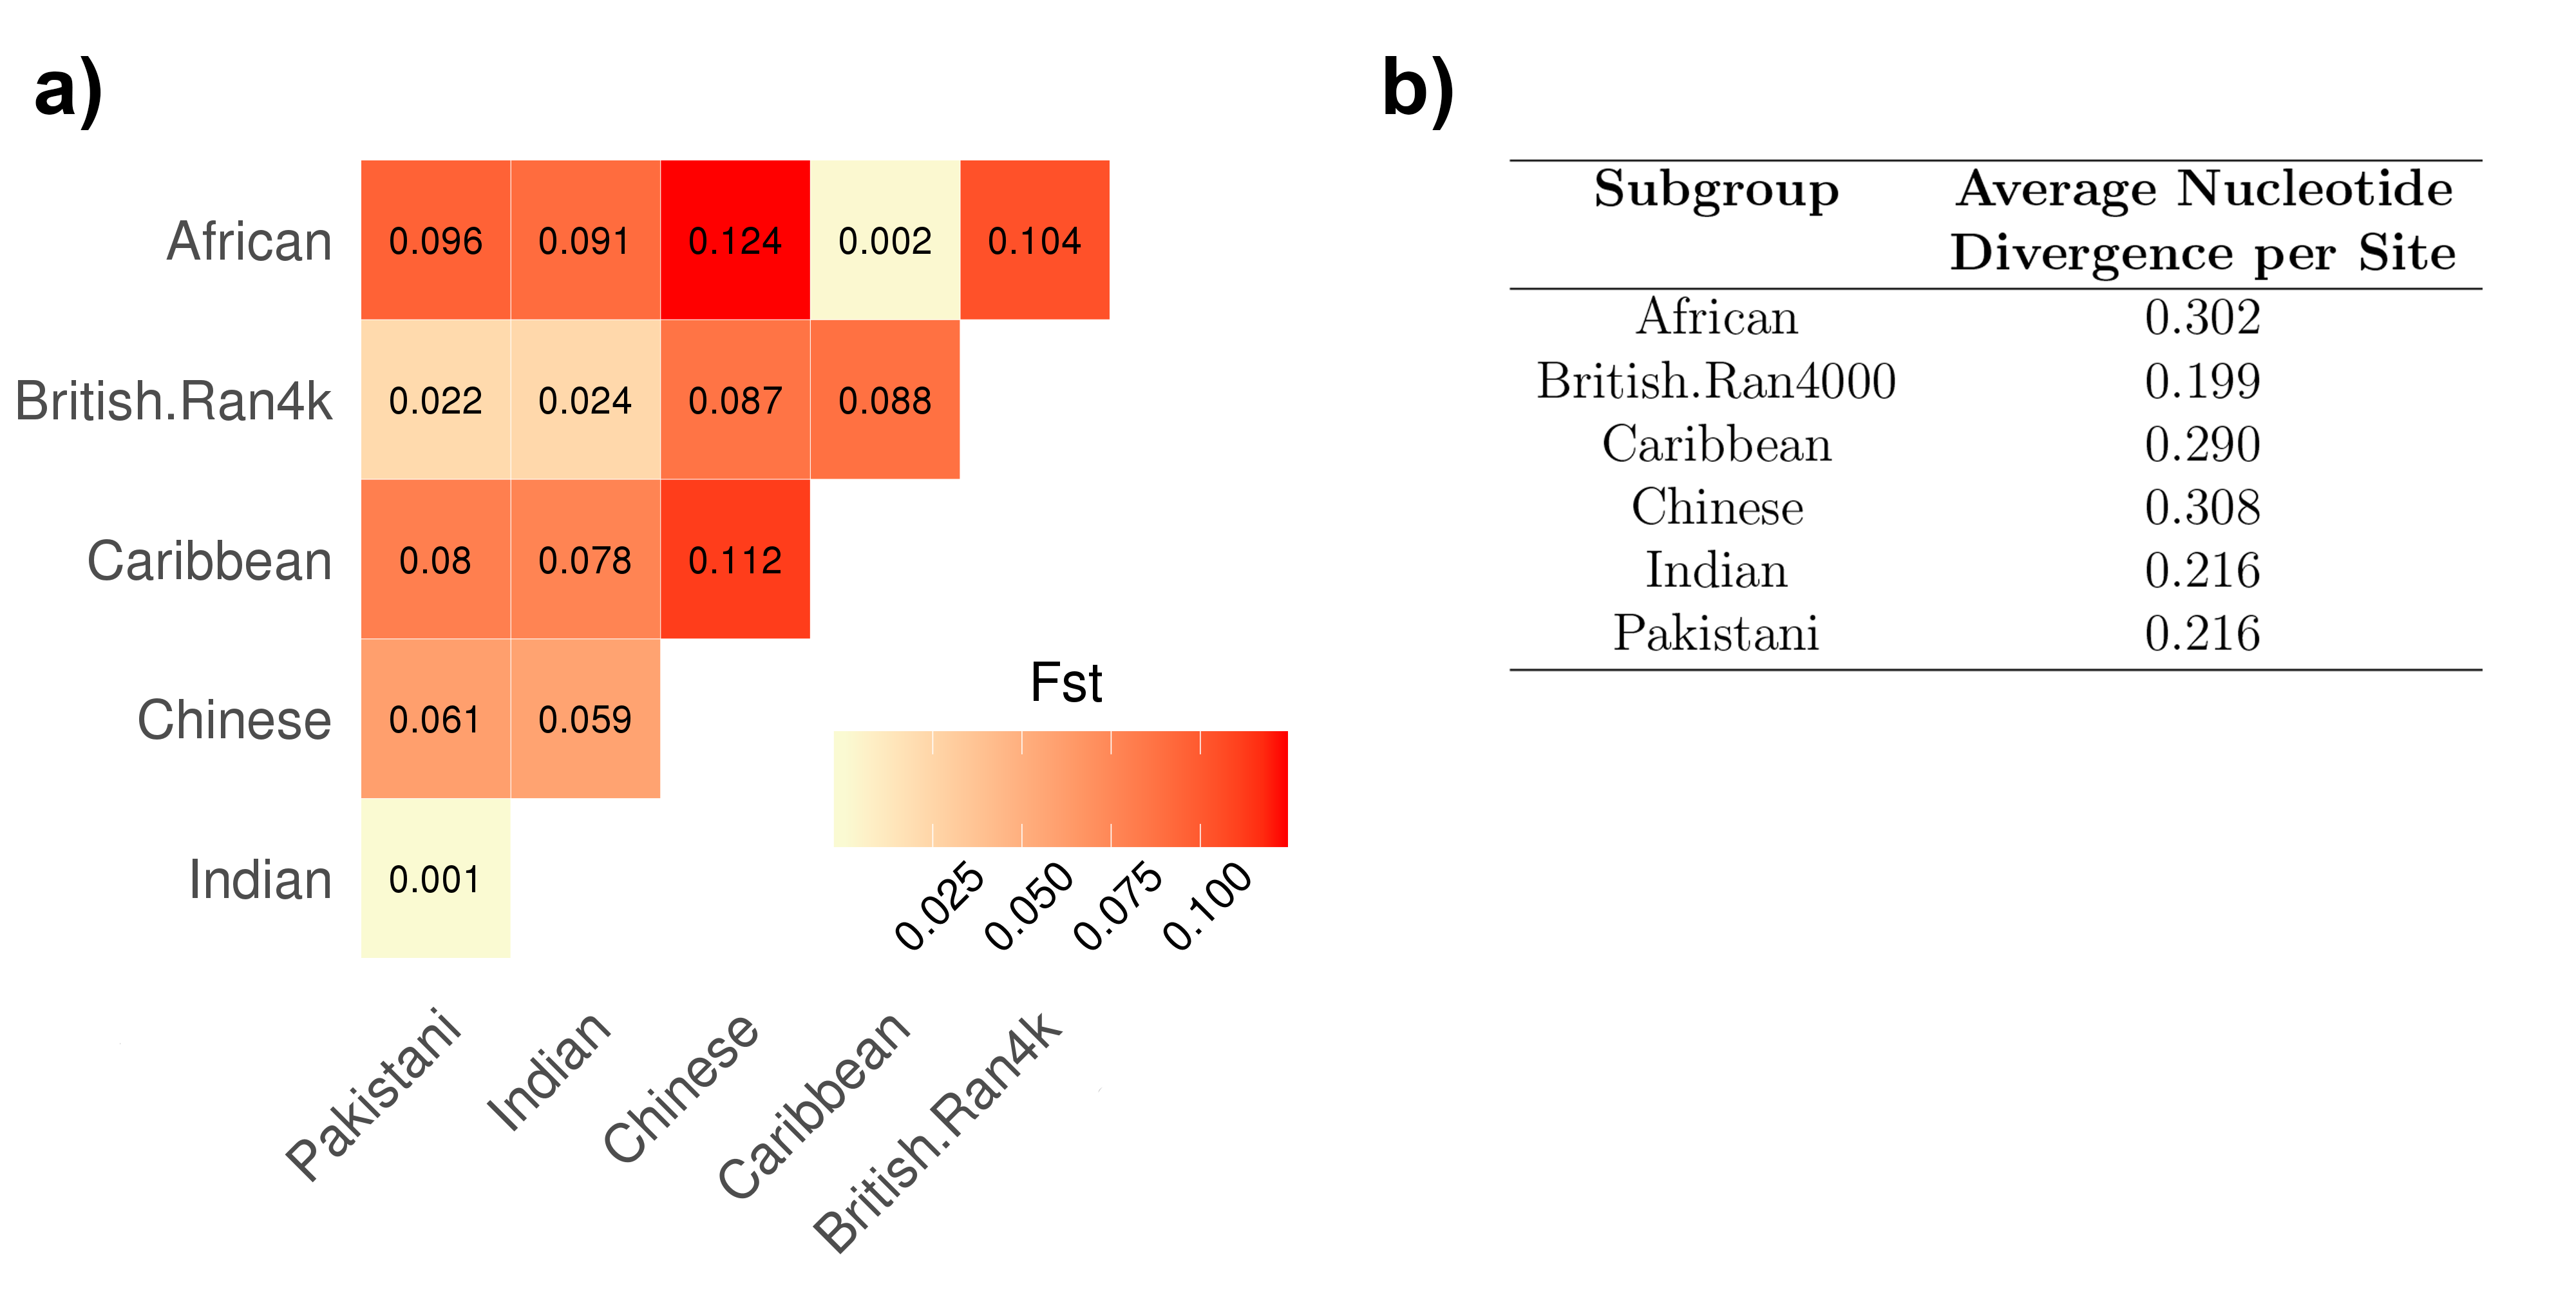
\includegraphics[scale=.5]{Images/Main/InterPath_Main_Figure_Fst_vs3.png}
\caption[TBD]{\textbf{Between- and within-UKB subgroup genetic variation estimates}. (a) The heatplot shows pairwise F\textsubscript{ST} values between each of our UKB population subgroups using the genome-wide SNP data. (b) The table shows the average nucleotide divergence per site for each presented subgroup.}
\label{InterPath-Main-Figure-Fst}
\end{figure}

%These global patterns, however, do not match the distribution of total number of significant MAPIT-R pathways observed per-ancestry in Figure \ref{InterPath-Main-Figure-Barplots-KEGG} and Supplementary Figure \ref{InterPath-Supp-Figure-Barplots-REACTOME}.

To test whether localized signatures of genetic variation influence our MAPIT-R results, we calculated a pathway-level metric of within-subgroup genetic variation, the mean pairwise proportion of identity-by-state (IBS) per pathway;  specifically, for each pathway, we calculated the proportion of IBS between every pair of individuals within a given subgroup using the SNPs in that pathway and then took the average of this proportion across all pairwise comparisons.  Comparing this per-pathway metric of within-subgroup genetic variation against each pathway's MAPIT-R $p$-value then, we find that there is no significant relationship between the two (Figure \ref{InterPath-Main-Figure-IBS-African} \& Supplementary Figure \ref{InterPath-Supp-Figure-IBS-AllPops}). Figure \ref{InterPath-Main-Figure-IBS-African} shows the analysis specifically for the African subgroup in the REACTOME database for both height and BMI, but this lack of relationship is observed for the majority of our pathway database-phenotype-UKB subgroup combinations (Supplementary Figure \ref{InterPath-Supp-Figure-IBS-AllPops}). 

%And in directly comparing these analyses between subgroups, we observe that specific differences between pathways are similar across subgroups; subgroups are shifted by their average level of mean proportion of pairwise IBS per pathway, but otherwise no clear ancestry-specific patterns are seen. (Figure \ref{InterPath-Main-Figure-IBS-AllPopComps-KEGG} \& Supplementary Figure \ref{InterPath-Supp-Figure-IBS-AllPopComps-REACTOME}). 

\begin{figure}[htb]
\centering
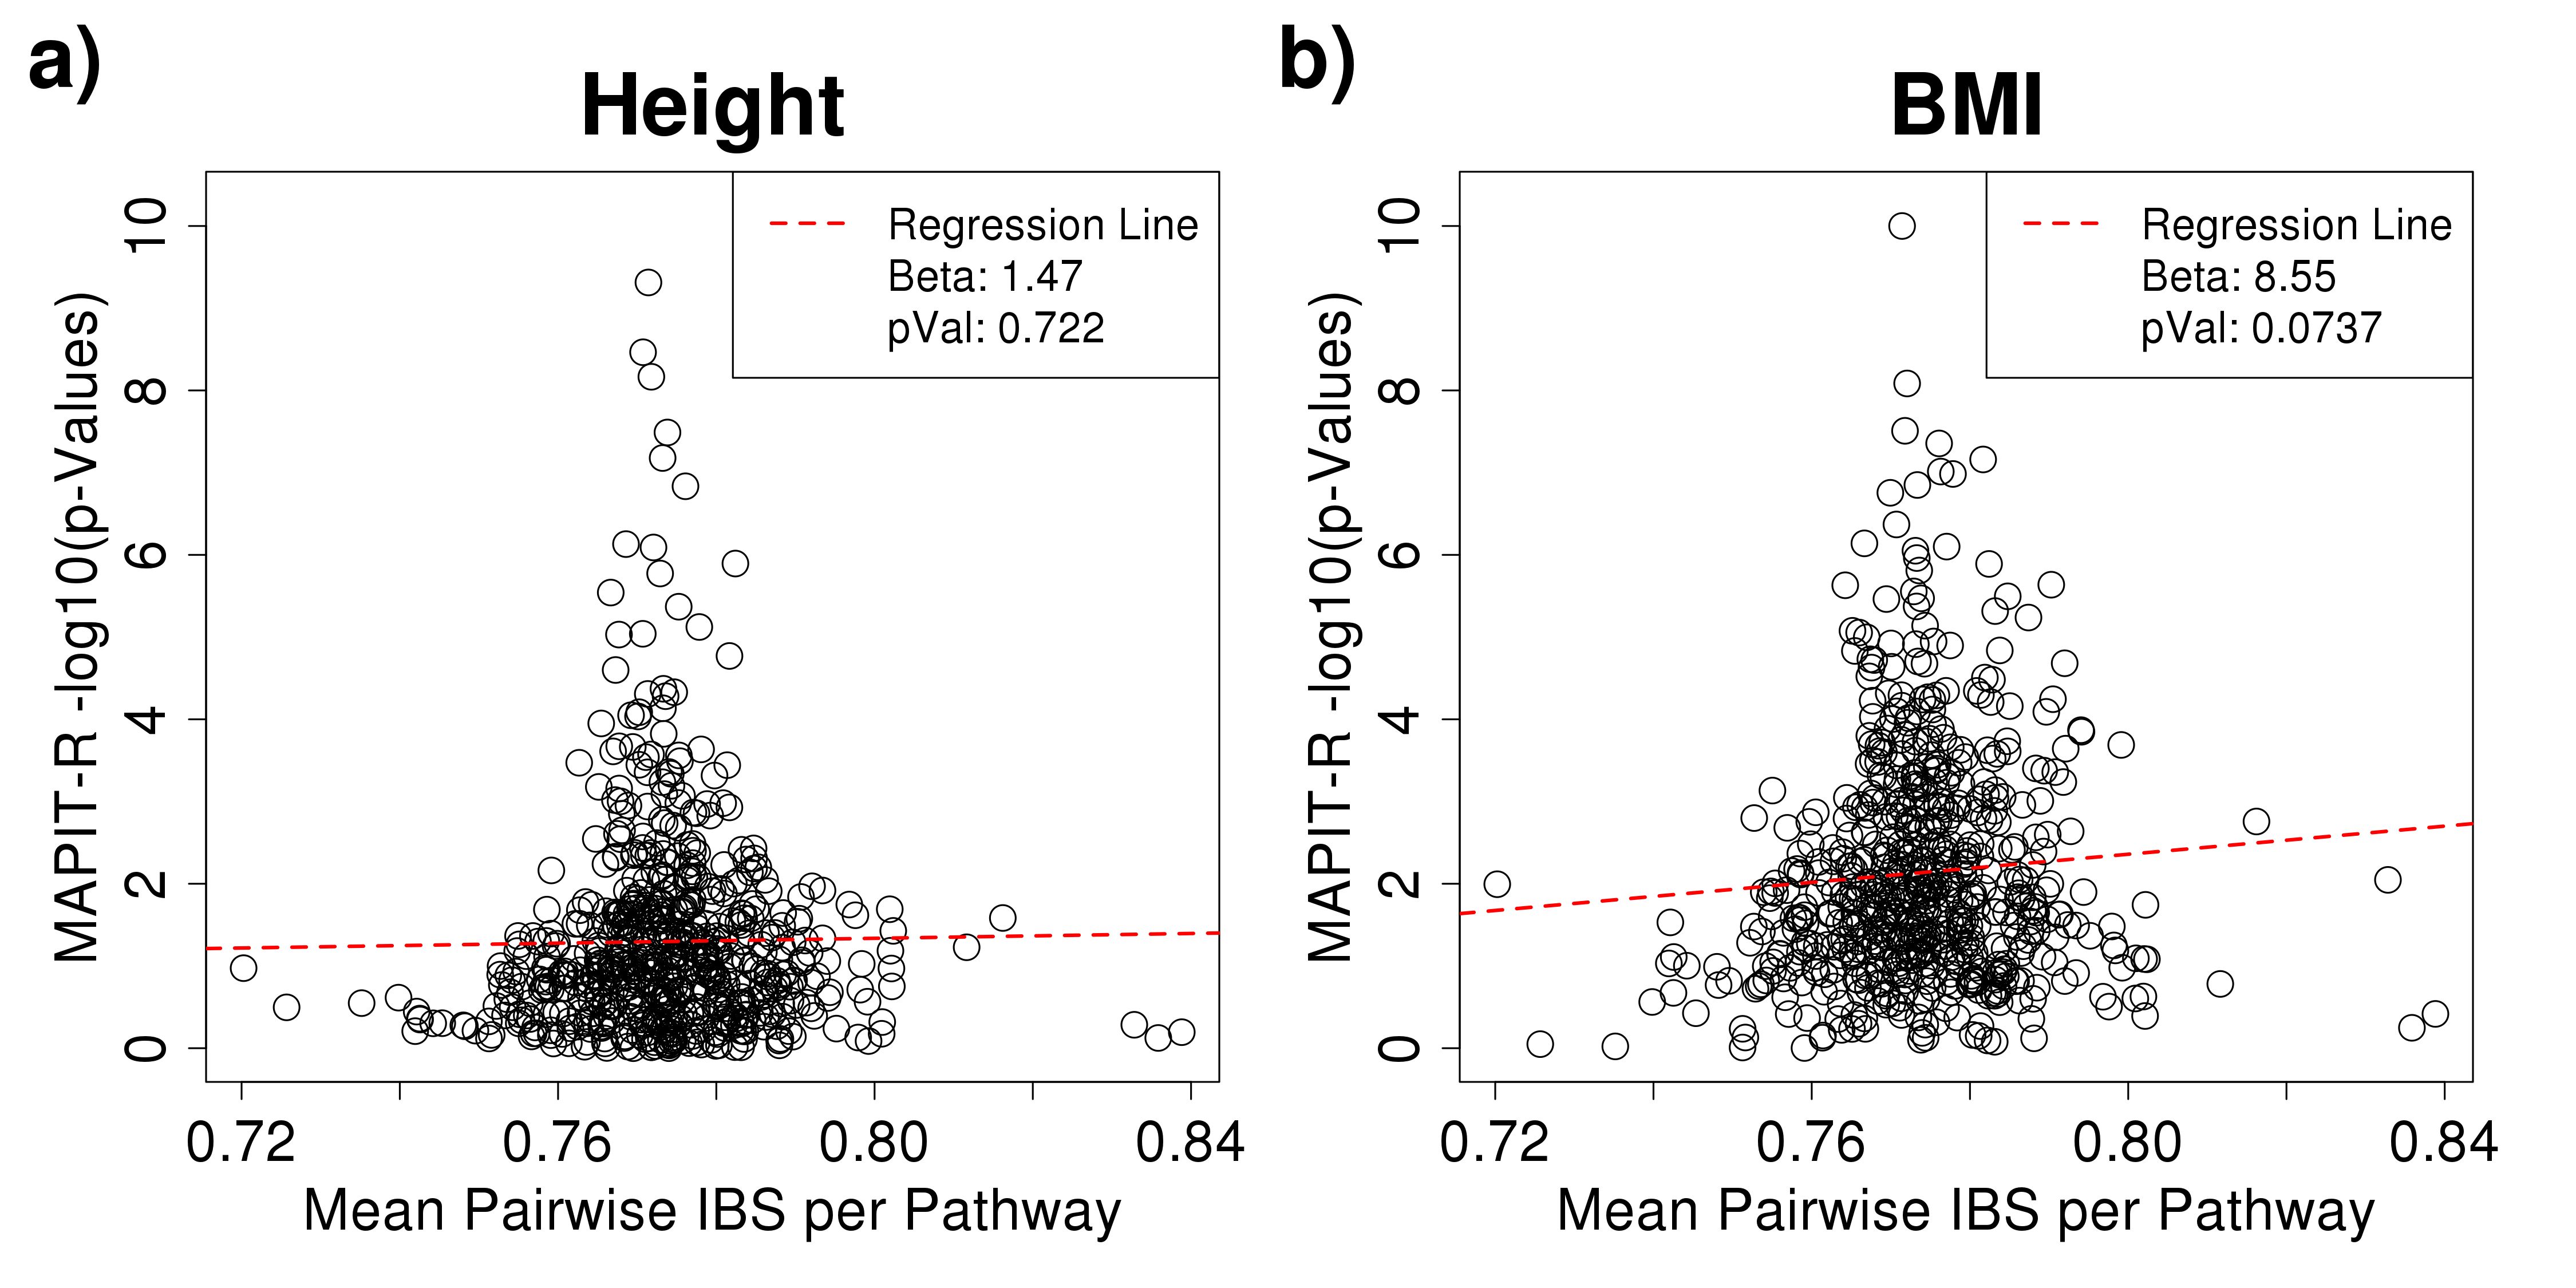
\includegraphics[scale=.35]{Images/Main/InterPath_Main_Figure_IBS_vs4_African_REACTOME_noHLA.png}
\caption[TBD]{\textbf{MAPIT-R results vs. pathway-level genetic diversity in the African subgroup and REACTOME database}. The figure shows MAPIT-R $p$-values per pathway plotted against each pathway's mean pairwise IBS proportions for the African subgroup REACTOME (a) height and (b) BMI analyses. Mean pairwise IBS proportions are shown on the $x$-axis and MAPIT-R $p$-values are shown on the $y$-axis. IBS proportions were calculated per pathway by using each pathway's set of SNPs to derive pairwise IBS values between every set of individuals in the subgroup, and then averaging across each of these pairs for a final summary metric. Results for each database-phenotype-subgroup combination can be found in Supplementary Figure \ref{InterPath-Supp-Figure-IBS-AllPops}.}
\label{InterPath-Main-Figure-IBS-African}
\end{figure}

Since neither whole-genome or pathway-level metrics of genetic variation appear to drive MAPIT-R results, we instead looked at more direct estimates of African ancestry rather than genetic variation as a proxy for African ancestry. Specifically, we ran RFMix \citep{Maples2013} on our African subgroup with the 1000 Genomes CEU and YRI \citep{Genomes2015} populations as outgroups to calculate per individual estimates of local African ancestry and then derived subgroup-wide average local ancestry estimates across all individuals. By comparing the average overlap a pathway has on African ancestry regions of the genome against that pathway's MAPIT-R $p$-value, we might identify regions of the genome that are both driving the MAPIT-R results but also doing so in an African-ancestry specific way. We did not identify a significant relationship between a pathway's MAPIT-R $p$-value and the average amount of local African ancestry in that pathway in the African subgroup  (Figure \ref{InterPath-Main-Figure-RFMix-African-REACTOME} and Supplementary Figure \ref{InterPath-Supp-Figure-RFMix-African-KEGG}).    

\begin{figure}[htb]
\centering
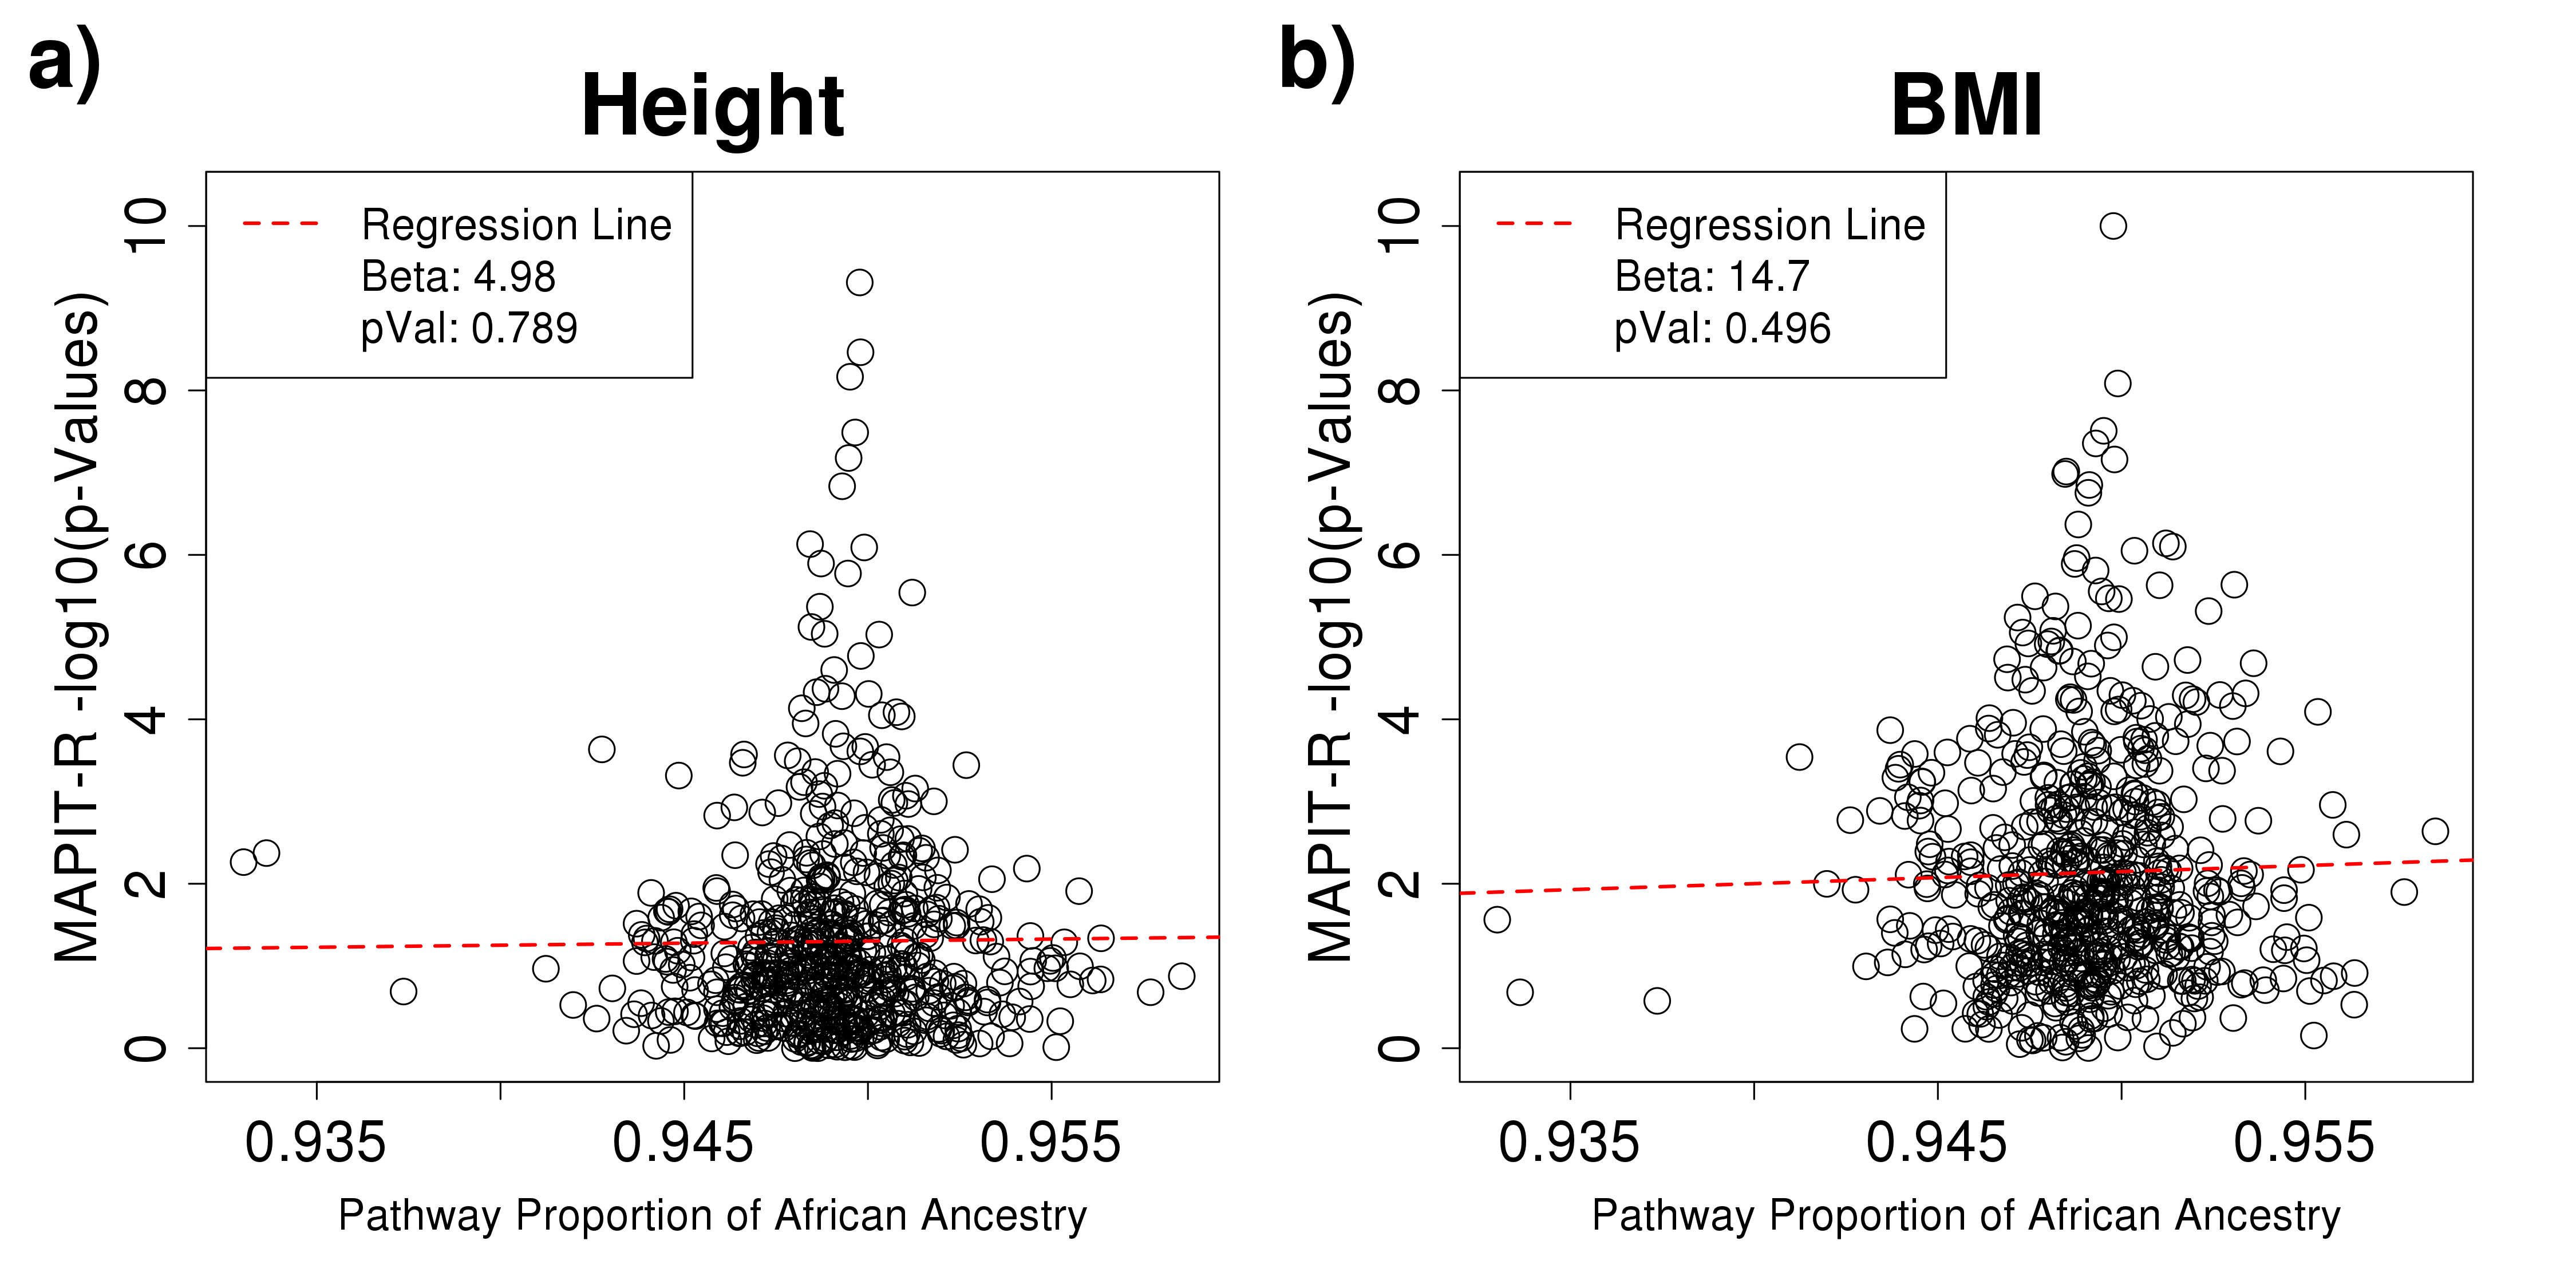
\includegraphics[scale=.35]{Images/Main/InterPath_Main_Figure_RFMix_vs2_African_REACTOME_noHLA.png}
\caption[TBD]{\textbf{MAPIT-R results vs. proportion of local African ancestry per REACTOME pathway}. The figure shows MAPIT-R $p$-values per pathway plotted against each pathway's proportion of local African ancestry for each REACTOME (a) height and (b) BMI analysis. Proportions of African ancestry are shown on the $x$-axis and MAPIT-R $p$-values are shown on the $y$-axis. African ancestry proportions were calculated per individual by using RFMix with the 1000 Genomes CEU and YRI populations as outgroups and then genome-wide averages were taken across the subgroup. Per pathway proportions of African ancestry were derived by taking the average of the subgroup-wide estimates of African ancestry across the regions of the genome that each pathway overlapped.}
\label{InterPath-Main-Figure-RFMix-African-REACTOME}
\end{figure}

We tested whether cryptic patterns of genetic variation, such as genetic variation patterns observed in principal component space, might be correlated with MAPIT-R $p$-values. Principal components could capture more multidimensional patterns of variation and provide direction on which areas of the genome to further explore for epistatic interactions. We examined the  proportion of variance explained (PVE) of the top 10 local PCs for each subgroup to see if there were any patterns that aligned with the number of significant MAPIT-R results we observe per subgroup. Figure \ref{InterPath-Main-Figure-Eigenvalues} demonstrates that PVE explained by the first principal component in each ancestry has a distribution across ancestries qualitatively similar to the rank order of significant MAPIT-R results per subgroup.



Next, we compared the proportion of SNPs that are strongly loaded on PC1 within a given pathway against that pathway's MAPIT-R $p$-value. If the cryptic structure represented by PC1 is driving the African MAPIT-R results, then we might expect pathways with more SNPs that are strongly loaded on PC1 to have more significant MAPIT-R $p$-values as well. To assess this, we projected every SNP back onto the local PC space derived for the MAPIT-R analyses, and defined a SNP as `strongly loaded' on PC1 if it had a loading score within the 2.5\% tails of the full PC1 loading score distribution. We then found the proportion of `strongly loaded' SNPs that were present in every pathway to have a final pathway-level metric. However, after comparing these values to MAPIT-R $p$-values, we once again find no relationship. Testing MAPIT-R pathway $p$-values against each pathway's proportion of `strongly loaded' PC1 SNPs shows no significantly positive relationship across any of our database-phenotype-subgroup combinations (Supplementary Figure \ref{InterPath-Supp-Figure-PC1Loading-AllPaths}). 

\fi

\end{document}
